\documentclass[12pt]{report}

\linespread{1.5}
\usepackage[margin=1.0in]{geometry}

%\interdisplaylinepenalty=2500
%\pretolerance=150


\setcounter{secnumdepth}{3}
\setcounter{tocdepth}{3}

\usepackage{amsmath,amssymb,amsfonts}
\usepackage{algorithmic}
\usepackage{graphicx}
\usepackage{textcomp}
\usepackage{bm}
\usepackage{upgreek}

\usepackage[retainorgcmds]{IEEEtrantools}

\usepackage{hyperref}

\usepackage[colorinlistoftodos,color=yellow!50,linecolor=red]{todonotes}
\newcommand{\todolow}[1]{\todo[inline,color=blue!50,linecolor=red]{#1}}
\newcommand{\todolo}[1]{\todo[inline,color=green!50,linecolor=red]{#1}}
\newcommand{\todomid}[1]{\todo[inline,color=yellow!50,linecolor=red]{#1}}
\newcommand{\todohi}[1]{\todo[inline,color=orange!50,linecolor=red]{#1}}
\newcommand{\todohigh}[1]{\todo[inline,color=red!50,linecolor=red]{#1}}


\usepackage{fancyhdr}
\pagestyle{fancy}
\fancyhf{}
\lhead{\leftmark}
\rhead{\thepage}
\renewcommand{\headrulewidth}{2pt}
%\renewcommand{\footrulewidth}{1pt}



\DeclareMathOperator*{\argmin}{arg\,min}
\DeclareMathOperator*{\argmax}{arg\,max}

%\newcommand{\diag}{\mathop{\rm diag}}
\DeclareMathOperator{\diag}{\mathrm{diag}}

\DeclareMathOperator{\xrm}{\mathrm{x}}
\DeclareMathOperator{\Xrm}{\mathrm{X}}
\DeclareMathOperator{\yrm}{\mathrm{y}}
\DeclareMathOperator{\Yrm}{\mathrm{Y}}
\DeclareMathOperator{\Drm}{\mathrm{D}}
\DeclareMathOperator{\nrm}{\mathrm{n}}
\DeclareMathOperator{\zrm}{\mathrm{z}}

\DeclareMathOperator{\Prm}{\mathrm{P}}
\DeclareMathOperator{\prm}{\mathrm{p}}
\DeclareMathOperator{\Erm}{\mathrm{E}}
\DeclareMathOperator{\Crm}{\mathrm{C}}
\DeclareMathOperator{\drm}{\mathrm{d}}

\DeclareMathOperator{\Xcal}{\mathcal{X}}
\DeclareMathOperator{\Ycal}{\mathcal{Y}}
\DeclareMathOperator{\Dcal}{\mathcal{D}}
\DeclareMathOperator{\Ncal}{\mathcal{N}}
\DeclareMathOperator{\Zcal}{\mathcal{Z}}
\DeclareMathOperator{\Hcal}{\mathcal{H}}
\DeclareMathOperator{\Fcal}{\mathcal{F}}
\DeclareMathOperator{\Rcal}{\mathcal{R}}
\DeclareMathOperator{\Mcal}{\mathcal{M}}
\DeclareMathOperator{\Scal}{\mathcal{S}}
\DeclareMathOperator{\Pcal}{\mathcal{P}}
\DeclareMathOperator{\Lcal}{\mathcal{L}}

\DeclareMathOperator{\Rbb}{\mathbb{R}}
\DeclareMathOperator{\Rbbgeq}{\mathbb{R}_{\geq 0}}
\DeclareMathOperator{\Nbb}{\mathbb{N}}
\DeclareMathOperator{\Zbb}{\mathbb{Z}}
\DeclareMathOperator{\Zbbgeq}{\mathbb{Z}_{\geq 0}}

\DeclareMathOperator{\Dir}{\mathrm{Dir}}
\DeclareMathOperator{\DM}{\mathrm{DM}}
\DeclareMathOperator{\Multi}{\mathrm{Multi}}
\DeclareMathOperator{\Bi}{\mathrm{Bi}}
\DeclareMathOperator{\DP}{\mathrm{DP}}
\DeclareMathOperator{\DMP}{\mathrm{DMP}}
\DeclareMathOperator{\Emp}{\mathrm{Emp}}
\DeclareMathOperator{\DE}{\mathrm{DE}}
\DeclareMathOperator{\EP}{\mathrm{EP}}
\DeclareMathOperator{\DEP}{\mathrm{DEP}}

\DeclareMathOperator{\thetam}{\theta_\text{m}}
\DeclareMathOperator{\upthetam}{\uptheta_\text{m}}
\DeclareMathOperator{\thetac}{\theta_\text{c}}
\DeclareMathOperator{\upthetac}{\uptheta_\text{c}}

\DeclareMathOperator{\psim}{\psi_\text{m}}
\DeclareMathOperator{\Psim}{\Psi_\text{m}}
\DeclareMathOperator{\uppsim}{\uppsi_\text{m}}
\DeclareMathOperator{\Uppsim}{\Uppsi_\text{m}}
\DeclareMathOperator{\psic}{\psi_\text{c}}
\DeclareMathOperator{\Psic}{\Psi_\text{c}}
\DeclareMathOperator{\uppsic}{\uppsi_\text{c}}
\DeclareMathOperator{\Uppsic}{\Uppsi_\text{c}}

\DeclareMathOperator{\alpham}{\alpha_\text{m}}
\DeclareMathOperator{\alphac}{\alpha_\text{c}}

\DeclareMathOperator{\gammam}{\gamma_\text{m}}


\usepackage[backend=biber,style=numeric]{biblatex}
\addbibresource{../References/PhD_refs.bib}

\graphicspath{{../Figures/}}

\title{Bayesian Learning using a Dirichlet Prior for Regression and Classification}
\author{Paul Rademacher}
%\date{}


\begin{document}

\maketitle
\tableofcontents


\newpage

\listoftodos



\todolow{use todonotes package instead of my initials?}

\todolow{equation numbers to final line!}

\todolow{brackets for expectation ops?}

\todolow{line break symbol format, before/after?}

\todomid{Is Dir and DP redundant?? DM and DMP?}

\todolo{likelihood function terminology}

\todomid{Dirichlet localization or concentration?}

\todolow{DIM and PR and LIM operators from AMS?}

\todolow{Ditch PMF/PDF case? roman?}

\todolo{Operator/functional terminology?}


\todohi{outer product, diag operators!! fix arguments}

\todohigh{HALDANE PRIOR}




\todohigh{ALL figure notation: theta font + Ycal indexing. use R,f opt?}

\todomid{Use $\Pcal$ only? Define discrete version of $\Pcal$?}

\todolo{use clairvoyant/irreducible terms and symbols $\Rcal$}

\todolo{suppress arguments where sensible? eg Pd = theta}

\todomid{reconsider irreducible terminology}

\todomid{empirical risk terms/discussion?}



\todohigh{Generalize to semi-supervised joint decisions??? training/test!}

\todohi{Investigate N lim for psi given theta, risks. Model support, bounded prior?}

\todohi{priors = sparse conditionals; w/ sufficient statistics}


\todolow{NFLT investigation? try sim examples}

\todolow{generalize y,x,h from scalars to functions!!!}

\todolow{jeffrey prior, fisher info?}




\todolow{bibliography}

Theo: (mult moments), DP agg, Dir moments

Bishop: (dir eq), dir posterior, moments, mode

Ferguson: (agg Dir), agg DP - via theo, DP posterior, moments

Gershman: agg DP - ref ferg, discrete draws

Johnson GET PDF: mult moments, (mult agg, DM agg, DM moments)

Add Theo-PR???

\newpage





\chapter{Introduction}


\section{Background}

PGR: complete rework!!

This report details a Bayesian perspective on statistical learning theory for when both the observations and unobserved quantities are jointly distributed according to an unknown probability distribution function. While the validity of Bayesian methods for statistical signal processing and machine learning has long been contended, the author believes it to be a justified approach that does not necessarily imply that the distribution model is `random'; rather, it simply reflects the desire of the user to formulate risk as a weighted sum of learner performance across the space of distributions. 

The success or failure of Bayesian learning methods hinge on how well the prior knowledge imparted by the designer matches reality. The chosen prior distribution over the set of data-generating probability distributions reflects the users confidence that different distributions are responsible for generating the observed/unobserved random elements. If a highly informative prior \cite{box} is chosen that is concentrated around the actual data probability distribution, low risk learning functions are possible even with limited training data; however, if the informative prior is poorly designed, a good solution may not be achieved. Conversely, a non-informative prior that weights the different distributions without preference provides a more robust solution for all models, but may underperform relative to learners based on well-selected informative priors.

This work assumes that the prior distribution is Dirichlet. The class of Dirichlet probability density functions (PDF) and processes have the desirable properties of full support over the set of possible data-generating distributions and an analytic posterior distribution for independently and identically distributed data \cite{ferguson}. Furthermore, control of the Dirichlet parameters can enable both non-informative and informative prior knowledge. Special cases including the uniform prior will be given specific attention.

After introducing the problem and discussing the relevant data probability distributions, the Bayesian framework will be applied to two of the most common loss functions in machine learning: the squared error loss function (common for regression), and the 0-1 loss function \cite{berger} (common for classification). Optimal estimators/classifiers and their corresponding minimum risk will be presented for different Dirichlet prior distributions. Specific attention will be given to various asymptotic cases to show the differing performance for non-informative and informative Dirichlet priors.




\section{Notation}

\todolo{Discuss arithmetic ops on functions? Upcasting?!}

This section details the mathematical notation and typesetting conventions used throughout. Note that many variable scalars and functions including $x$, $y$, $g$, etc. are repeatedly redefined and reused to avoid introducing an excessive volume of symbols; unless explicitly stated, none of these variable definitions will hold in subsequent sections.


\subsection*{Sets and Function Arguments}

Sets will typically be typeset with a calligraphic font, such as $\Xcal$. Exceptions include common number sets such as the real numbers, which are typeset using blackboard bold $\Rbb$. Function spaces such as the set of functions $\Xcal \mapsto \Ycal$ are compactly represented as $\Ycal^{\Xcal}$.

\todolo{non-calligraphic for risk, loss, etc?}

Various mappings will be defined for which the domain and/or the range \cite{rudin} are function spaces. The set of functions $\Xcal \mapsto \Ycal$ is denoted $\Ycal^{\Xcal}$. For a mapping $g : \Zcal \mapsto \Ycal^{\Xcal}$, the argument notation $g(z) \in \Ycal^{\Xcal}$ denotes a function, while $g(x;z) \in \Ycal$ is a specific value of that function. Semicolons are used to distinguish between the arguments referring to the domain and arguments that access the resulting function. The mapping $\{1,\ldots,N\} \mapsto \Ycal$ will be represented as $\Ycal^N$ for brevity. Spaces of indexed tuples will be notated as $g \in \Ycal^N$ and items of a tuple are accessed with subscripts rather than parentheses, such that $g_i \in \Ycal$.

The Cartesian product of sets will be frequently used, such that for $x \in \Xcal$ and $y \in \Ycal$, the pair $(x,y) \in \Xcal \times \Ycal$. For a general product of sets $\Scal_i$, the notation $\prod_i \Scal_i = \Scal_1 \times \Scal_2 \ldots$ is used.

The convention adopted for natural numbers is $\Nbb = \{1,2,\ldots\}$; the set of non-negative integers is denoted $\Zbbgeq = \Nbb \cup \{0\}$. The set of positive real numbers $\Rbb^+$ excludes zero, while non-negative real numbers are represented as $\Rbbgeq = \Rbb^+ \cup \{0\}$. The cardinality of countably infinite sets, including the set of natural numbers, is denoted $\aleph_0 = |\Nbb|$; the cardinality of uncountable sets such as $\Rbb$ is at least $\aleph_1$.

Numerous probability distribution functions will be defined over different domains. As such, for a given set $\Xcal$, define a set function $\Pcal$ such that $\Pcal(\Xcal)$ is the set of distributions over $\Xcal$. If $\Xcal$ is countable, the set is defined as $\Pcal(\Xcal) = \left\{ p \in {\Rbbgeq}^{\Xcal}: \sum_{x \in \Xcal} p(x) = 1 \right\}$; if $\Xcal$ is a Euclidean space, the set is defined as $\Pcal(\Xcal) = \left\{ p \in {\Rbbgeq}^{\Xcal}: \int_{\Xcal} p(x) {\drm}x = 1 \right\}$.

\todolo{aleph reference?}



\subsection*{Special Operators and Functions}

Various operators commonly used in linear algebra will be generalized for functions. Specifically, the outer product operator $\otimes$ is used on two real-valued functions $f \in \Rbb^{\Xcal}$ and $g \in \Rbb^{\Ycal}$, such that $\big(f \otimes g\big) \in \Rbb^{\Xcal \times \Ycal}$ with $\big(f \otimes g\big) (x,y) = f(x) g(y)$. A general outer product of functions is denoted $\bigotimes_i f_i = f_1 \otimes f_2 \ldots$ for $i = 1,\ldots$, where $\Big(\bigotimes_i f_i\Big)(x_1,x_2,\ldots) = f_1(x_1)f_x(x_2)\ldots$, is used as well. Also, the diagonal operator operates on a single real-valued function, such that $\diag(f) \in \Rbb^{\Xcal \times \Xcal}$. For countable sets $\Xrm$, the operator values are $\diag(f)(x,x') = f(x) \delta[x,x']$; for Euclidean sets, the operator values are $\diag(f)(x,x') = f(x) \delta(x-x')$.

\todolow{tensor product?}


A variety of special functions will be used throughout. Both the Dirac and Kronecker delta functions will frequently required. The Dirac delta function over a Euclidean domain $\Xcal$ is represented as $\delta(\cdot)$; it has support only at the point $x=0$ and satisfies
\begin{equation}
	\int_{\Xcal} \delta(x) {\drm}x = 1 \;.
\end{equation}
Consequently, it also satisfies
\begin{equation}
	\int_{\Xcal} g(x) \delta(x) {\drm}x = g(0) \;.
\end{equation}
Consider a countable set $\Xcal$; the Kronecker delta function has domain $\Xcal \times \Xcal$ and is defined as
\begin{equation}
	\delta[x,x'] = \begin{cases} 1 & \mathrm{if} \ x = x', \\ 0 & \mathrm{if} \ x \neq x'.  \end{cases}
\end{equation}

\todolo{reference Dirac/Kronecker}

The multinomial coefficient and multivariate beta function, which typically operate on sequences, are defined more generally for function inputs. The multinomial operator $\Mcal$ is used for functions $g : \Xcal \mapsto \Zbbgeq$ that map to non-negative integers from an arbitrary countable domain $\Xcal$. The output of the operator is
\begin{equation}
	\Mcal(g) = \frac{\big( \sum_{x \in \Xcal} g(x) \big)!}{\prod_{x \in \Xcal} g(x)!} \;.
\end{equation}
Similarly, the beta function $\beta$ operates on functions $g : \Xcal \mapsto \Rbb^+$ that map to positive real numbers from an arbitrary countable domain $\Xcal$, such that
\begin{equation}
	\beta(g) = \frac{\prod_{x \in \Xcal} \Gamma\big( g(x) \big)}{\Gamma \left( \sum_{x \in \Xcal} g(x) \right)} \;.
\end{equation}
Note that the countable domains of the input functions may have an infinite number of elements. 

The indicator function $\chi$, defined as
\begin{equation}
	\chi(x;S) = \begin{cases} 1 & \mathrm{if} \ x \in S, \\ 0 & \mathrm{if} \ x \notin S \;, \end{cases}
\end{equation}
will be used repeatedly.




\subsection*{Random elements, variables, and processes}

Random elements are denoted with roman font (e.g. $\xrm$), while specific values are denoted with italics (e.g. $x$). Random elements that assume numerical scalars/functions are referred to as random variables/processes, respectively.

Consider a random element $\xrm \in \Xcal$. If $\Xcal$ is countable, either finite with $|\Xcal| \in \Nbb$ or countably infinite with $|\Xcal| = \aleph_0$, then $\xrm$ is a discrete random element and is characterized by a probability mass function (PMF) \cite {papoulis}, denoted $\Prm_{\xrm} \in \Pcal(\Xcal)$. If $\Xcal$ is a Euclidean space and is thus uncountable with $|\Xcal| \geq \aleph_1$, then $\xrm$ is a continuous random variable/process characterized by a probability density function (PDF), denoted $\prm_{\xrm} \in \Pcal(\Xcal)$.

\todolo{explicit PMF/PDF formula with P of events?}

Consider $\xrm$ conditioned on another random element $\zrm \in \Zcal$. The conditional distribution is represented as $\Prm_{\xrm | \zrm} : \Zcal \mapsto \Pcal(\Xcal)$, such that $\Prm_{\xrm | \zrm}(z)$ is a PMF over $\Xcal$ and $\Prm_{\xrm | \zrm}(x|z)$ is a specific value of that PMF. Often, the dependency on the conditional variable $\zrm$ will not be expressed in terms of a specific value $z$, but will be left in terms of the random element itself; in this case, the more compact notation $\Prm_{\xrm | \zrm}$ is used to imply $\Prm_{\xrm | \zrm}(\zrm)$, a function of $\zrm$.

\todohi{Ever need the full functional?}

Many distributions will be repeatedly used and thus special functions will be defined for the PDF's and PMF's of interest. For example, consider a random process $\xrm \in \Xcal$ characterized by a Multinomial distribution with parameters $N \in \Zbbgeq$ and $\theta \in \Uptheta$; the PDF will be notated as $\Multi : \Zbbgeq \times \Uptheta \mapsto \Pcal(\Xcal)$, where the range is the set of valid PDF's. More compactly, the notation $\xrm \sim \Multi(N, \theta)$ implies that $\Prm_{\xrm} = \Multi(N, \theta)$. Other distribution functions repeatedly used include $\Dir$, $\DE$, $\DP$, and $\DEP$, representing the Dirichlet distribution, the Dirichlet-Empirical distribution, the Dirichlet process, and the Dirichlet-Empirical process.

\todolo{Add PDF citations. Introduce Empirical process?}



\subsection*{Expectation Operators}

For a discrete random element $\xrm$, the expectation operator $\Erm_{\xrm}$ is defined as
\begin{equation}
\Erm_{\xrm}\big[ g(\xrm) \big] = \sum_{x} \Prm_{\xrm}(x) g(x) \;,
\end{equation}
where the argument $g$ is an arbitrary scalar function of $\xrm$ with range $\Rbb$. Additionally, define the variance operator $\Crm_{\xrm}$ as
\begin{equation}
\Crm_{\xrm}\big[g(\xrm)\big] = \Erm_{\xrm} \bigg[ \Big( g(\xrm) - \Erm_{\xrm}\big[g(\xrm)\big] \Big)^2 \bigg] \;.
\end{equation}
When $\xrm$ is a random variable and the function $g$ is the identity operator, such that $g(\xrm) = \xrm$, the mean and variance are compactly represented as $\mu_{\xrm}$ and $\Sigma_{\xrm}$, respectively.

These operations can be performed with respect to a conditional distribution as well. In this case, the expectation operator is a function of the observed value of $\zrm$, such that
\begin{equation}
\Erm_{\xrm | \zrm}\big[ g(\xrm) \big](z) = \sum_{x} \Prm_{\xrm | \zrm}(x | z) g(x) \;.
\end{equation}
Similarly, the conditional variance is notated $\Crm_{\xrm | \zrm}\big[ g(\xrm) \big](z)$. When $g$ is the identity operator, the conditional mean and variance as represented by $\mu_{\xrm | \zrm}(z)$ and $\Sigma_{\xrm | \zrm}(z)$, respectively.

As with conditional distributions, it is common that an explicit value $z$ of the conditional random element will not be used, but rather the expectation will be left as a function of the random element $\zrm$. In these cases, the argument is suppressed and the notation $\Erm_{\xrm | \zrm}\big[ g(\xrm) \big]$ implies the dependency on $\zrm$. This convention also holds for the conditional variance operator $\Crm_{\xrm | \zrm}$, as well as for the $\mu_{\xrm | \zrm}$ and $\Sigma_{\xrm | \zrm}$ functions.

If the range of $g$ is a Hilbert space, such that $g(\xrm)$ is itself a function with a domain $\Ycal$, then the notation for these operators is expanded. The output of the expectation operator is a function over $\Ycal$ represented by
\begin{equation}
\Erm_{\xrm}\big[ g(\xrm) \big](y) = \sum_{x} \Prm_{\xrm}(x) g(y;x) \;.
\end{equation}
Similarly, the covariance function notation is modified and the output is a function over $\Ycal \times \Ycal$, 
\begin{IEEEeqnarray}{L}
\Crm_{\xrm}\big[g(\xrm)\big](y,y') = \Erm_{\xrm} \bigg[ \Big( g(y;\xrm) - \Erm_{\xrm}\big[g(y;\xrm)\big] \Big) \Big( g(y';\xrm) - \Erm_{\xrm}\big[g(y';\xrm)\big] \Big) \bigg] \;.
\end{IEEEeqnarray}
\begin{IEEEeqnarray}{L}
\Crm_{\xrm}\big[g(\xrm)\big] = \Erm_{\xrm} \bigg[ \Big( g(\xrm) - \Erm_{\xrm}\big[g(\xrm)\big] \Big) \otimes \Big( g(\xrm) - \Erm_{\xrm}\big[g(\xrm)\big] \Big) \bigg] \;.
\end{IEEEeqnarray}
As before, the notation is simplified when the function $g$ is the identity operator. If $\xrm$ is a random process over a domain $\Ycal$, then the mean and covariance functions are defined over domains $\Ycal$ and $\Ycal \times \Ycal$ with values notated such as $\mu_{\xrm}(y)$ and $\Sigma_{\xrm}(y,y')$.

If the expectations are evaluated with respect to a conditional distribution $\Prm_{\xrm | \zrm}$, the additional argument for the observed random element is added and the notation for the above operators is extended to $\Erm_{\xrm|\zrm}\big[ g(\xrm) \big](y|z)$ and $\Crm_{\xrm|\zrm}\big[g(\xrm)\big](y,y'|z)$ for non-scalar outputs. When $g$ is the identity operator, the notation $\mu_{\xrm|\zrm}(y|z)$ and $\Sigma_{\xrm|\zrm}(y,y'|z)$ is used. As for probability distributions, it is common for the conditional random element $\zrm$ to be left as a random quantity instead of being explicitly defined; in these cases, the dependency on $\zrm$ is implied.


\todohi{BELOW NOTATION CREATES AMBIGUITY!!!!!!! Check for residual uses...}

In such cases, the italic $z$ is dropped from the arguments and the formulas $\Erm_{\xrm|\zrm}\big[ g(\xrm) \big](y)$, $\Crm_{\xrm|\zrm}\big[g(\xrm)\big](y,y')$, $\mu_{\xrm|\zrm}(y)$, and $\Sigma_{\xrm|\zrm}(y,y')$ imply dependence on $\zrm$.








\newpage

\chapter{Problem Statement}

\todohigh{REWORK TEXT}

\section{Data Model}

\todolow{italic theta font before Bayes?}

Consider an observable random element $\xrm \in \Xcal$ and an unobservable random element $\yrm \in \Ycal$ which are jointly distributed according to an unknown probability distribution $\uptheta \in \Uptheta \equiv \Pcal(\Ycal \times \Xcal)$, such that $\Prm_{\yrm,\xrm | \uptheta} = \uptheta$. Note that the uppercase PMF notation used throughout this section implies that the random elements are discrete; PDF's are used when $\xrm$ and/or $\yrm$ are continuous random variables/processes.

Also observed is a random sequence of $N$ samples from $\uptheta$, denoted $\Drm \in \Dcal = \{\Ycal \times \Xcal\}^N$; an alternative representation that can be used is $\Drm \Leftrightarrow \big( (\Yrm_1,\Xrm_1),\ldots,(\Yrm_N,\Xrm_N) \big)$, where $\Yrm \in \Ycal^N$ and $\Xrm \in \Xcal^N$. The $N$ data pairs are conditionally independent from one another and are identically distributed as $\Prm_{\Drm_n | \uptheta} = \Prm_{\yrm,\xrm | \uptheta}$. The samples are also conditionally independent from $(\yrm,\xrm)$. Thus $\Prm_{\yrm,\xrm,\Drm | \uptheta} = \Prm_{\yrm,\xrm | \uptheta} \otimes \left( \bigotimes_{n=1}^N \Prm_{\Drm_n | \uptheta} \right) = \uptheta \otimes \left( \bigotimes_{n=1}^N \uptheta \right)$, or explicitly,
\begin{equation}
\Prm_{\yrm,\xrm,\Drm | \uptheta}(y,x,D | \theta) = \Prm_{\yrm,\xrm | \uptheta}(y,x | \theta) \prod_{n=1}^N \Prm_{\Drm_n | \uptheta}\big(Y_n,X_n | \theta\big) \;.
\end{equation}



\subsection{Marginal and Conditional Model Distributions}

As only $\yrm$ is unobservable, it will be useful to alternatively represent the model distribution via the bijection $\uptheta \Leftrightarrow (\upthetam,\upthetac)$. First, introduce the marginal distribution $\upthetam \equiv \sum_{y \in \Ycal} \uptheta(y,\cdot) \in \Pcal(\Xcal)$; note that the summation is replaced by an integral when $\yrm$ is a continuous random variable. Next, introduce the conditional distributions $\upthetac \in \Pcal(\Ycal)^{\Xcal}$ defined as $\upthetac(x) \equiv \uptheta(\cdot,x) / \upthetam(x)$. Observe that $\Prm_{\xrm | \uptheta} \equiv \Prm_{\xrm | \upthetam} = \upthetam$ and $\Prm_{\yrm | \xrm, \uptheta} \equiv \Prm_{\yrm | \xrm, \upthetac} = \upthetac(\xrm)$.






\section{Sufficient Statistic: the Empirical Distribution}

\todohigh{continuous? empirical process?}

For countable sets $\Ycal$ and $\Xcal$, the distribution of $\Drm$ conditioned on the model can be formulated as
\begin{IEEEeqnarray}{rCl}
\Prm_{\Drm | \uptheta}\big( D | \theta \big) & = & \prod_{n=1}^N \Prm_{\Drm_n | \uptheta}\big( D_n | \theta \big) = \prod_{n=1}^N \theta(D_n) \\
& = & \prod_{y \in \Ycal} \prod_{x \in \Xcal} \theta(y,x)^{N \Psi(y,x;D)} \nonumber \\
& = & \left( \prod_{y \in \Ycal} \prod_{x \in \Xcal} \theta(y,x)^{\Psi(y,x;D)} \right)^N \nonumber \;,
\end{IEEEeqnarray}
where the dependency on the training data $\Drm$ is expressed though a transform function $\Psi : \Dcal \mapsto \Uppsi \subset \Uptheta$, where the range is 
\begin{IEEEeqnarray}{rCl}
\Uppsi & = & \left\{ \frac{n}{N} : n \in {\Zbbgeq}^{\Ycal \times \Xcal}, \ \sum_{y \in \Ycal} \sum_{x \in \Xcal} n(y,x) = N \right\} 
\end{IEEEeqnarray}
and the function is defined as
\begin{IEEEeqnarray}{rCl}
\Psi(D) & = & \frac{1}{N} \sum_{n=1}^N \delta \big[ \cdot,D_n \big] \\
& \equiv & \frac{1}{N} \sum_{n=1}^N \delta \left[ \cdot,Y_n \right] \delta \left[ \cdot,X_n \right] ?? \nonumber \;.
\end{IEEEeqnarray}
This function determines the empirical probability of the pair $(y,x)$. Note that the set $\Uppsi$ is a finite subset of $\Uptheta$ and thus that the empirical model $\Psi(\Drm)$ is a valid probability distribution.

The distribution $\Prm_{\Drm | \uptheta}$ depends on the training data $\Drm$ only through the transform $\Psi$; as such, it is useful to define a new random process $\uppsi \equiv \Psi(\Drm) \in \Uppsi$. It can be shown that $\Prm_{\Drm | \uppsi,\uptheta}$ is a uniform distribution over $\{D \in \Dcal: \Psi(D) = \uppsi\}$ and thus that the empirical model $\uppsi$ is a sufficient statistic \cite{bernardo} for the model $\uptheta$.  

\todomid{show SS via Kay, data likelihood?! D AND x?}

The cardinality of the random process' domain is $|\Uppsi| = \Mcal\big( (N,|\Ycal||\Xcal|-1) \big)$; this can be shown using the stars-and-bars method \cite{feller}. The cardinality of original set is $|\Dcal| = \big( |\Ycal| |\Xcal| \big)^N$; thus $|\Uppsi| \leq |\Dcal|$ and the sufficient statistic compactly represents the valuable information in the training data. 

\todolo{sufficient statistic savings in memory bits?}

Conditioned on the model $\uptheta$, the PMF of $\uppsi$ is 
\begin{IEEEeqnarray}{rCl}
\Prm_{\uppsi | \uptheta}(\psi | \theta) & = & \sum_{D \in \{\Psi(D) = \psi\}} \Prm_{\Drm | \uptheta}(D | \theta) \\
& = & \big|\{ D : \Psi(D) = \psi \}\big| \prod_{y \in \Ycal} \prod_{x \in \Xcal} \theta(y,x)^{N \psi(y,x)} \nonumber \\
& = & \Mcal(N \psi) \prod_{y \in \Ycal} \prod_{x \in \Xcal} \theta(y,x)^{N \psi(y,x)} \nonumber \\
& = & \Multi\big( N \psi;N,\theta \big) \nonumber \\
& = & \Mcal(N \psi) \left( \prod_{y \in \Ycal} \prod_{x \in \Xcal} \theta(y,x)^{\psi(y,x)} \right)^N \nonumber \\
& = & \Emp\big( \psi;N,\theta \big) \nonumber \;.
\end{IEEEeqnarray}
Observe that the Empirical process is equivalent to a Multinomial process within a scale factor.

The first and second joint moments of this Empirical distribution (derived from Multinomial moments \cite{theodoridis-ML}) are
\begin{IEEEeqnarray}{rCl}
\mu_{\uppsi | \uptheta} & = & \uptheta
\end{IEEEeqnarray}
and
\begin{IEEEeqnarray}{L}
\Erm_{\uppsi | \uptheta}\big[ \uppsi \otimes \uppsi \big] = \frac{1}{N} \diag(\uptheta)  + \left(1 - \frac{1}{N}\right) \uptheta \otimes \uptheta 
\end{IEEEeqnarray}
%\begin{IEEEeqnarray}{L}
%\Erm_{\uppsi | \uptheta}\big[ \uppsi(y,x) \uppsi(y',x') \big] = \frac{1}{N} \uptheta(y,x) \delta[y,y'] \delta[x,x'] + \left(1 - \frac{1}{N}\right) \uptheta(y,x) \uptheta(y',x') 
%\end{IEEEeqnarray}
and the covariance function is
\begin{IEEEeqnarray}{rCl}
\Sigma_{\uppsi | \uptheta} & = & \frac{1}{N} \big( \diag(\uptheta) - \uptheta \otimes \uptheta \big) \;.
\end{IEEEeqnarray}
%\begin{IEEEeqnarray}{rCl}
%\Sigma_{\uppsi | \uptheta}(y,x,y',x' | \theta) & = & \frac{1}{N} \big( \theta(y,x) \delta[y,y'] \delta[x,x'] - \theta(y,x) \theta(y',x') \big) \;.
%\end{IEEEeqnarray}
The first and second moments of the Empirical distribution are proportionate to those of the Multinomial distribution.

Observe that for larger training data volumes $N$, the set $\Uppsi$ becomes a denser grid of samples from the set $\Uptheta$ and the covariance tends to zero, concentrating the Empirical PMF around the model $\uptheta$. Thus, as $N \to \infty$, 
\begin{equation}
\Prm_{\uppsi | \uptheta}(\psi | \theta) \to \delta[\psi, \theta] \;.
\end{equation}
This trend underscores the identifiability of the model $\theta$.

\todohigh{CHECK!???? SCALING FACTOR???}

\todohi{FIGS!}

\todomid{Cite Glivenko–Cantelli theorem?}

Also, using the maximum likelihood estimate of a Multinomial distribution \cite{rao}, the maximum likelihood estimate of $\theta$ given the training data empirical model is simply
\begin{IEEEeqnarray}{rCl}
\theta_\mathrm{ML}\big( \psi \big) & = & \argmax_{\theta \in \Uptheta} \Prm_{\uppsi | \uptheta}(\psi | \theta) = \psi \;.
\end{IEEEeqnarray}





\subsection{Marginal and Conditional Data Distributions}

Also of interest are the marginal and conditional distributions of the joint training data sequences $\Yrm$ and $\Xrm$. The marginal distribution given $\uptheta$ for the observations $\Xrm$ alone is
\begin{IEEEeqnarray}{rCl}
\Prm_{\Xrm | \uptheta}\big( X | \theta \big) & = & \prod_{n=1}^N \Prm_{\Xrm_n | \uptheta}\big( X_n | \theta \big) \equiv \prod_{n=1}^N \thetam(X_n) \\
& \equiv & \prod_{x \in \Xcal} \thetam(x)^{N \Psim(x;X)} \nonumber \\
& = & \left( \prod_{x \in \Xcal} \thetam(x)^{\Psim(x;X)} \right)^N \nonumber \;,
\end{IEEEeqnarray}
where the dependency on $\uptheta$ is only through the marginal model $\upthetam$. Additionally, note that the dependency on the training observations $\Xrm$ is expressed though a ``marginal'' distribution function $\Psim : \Xcal^N \mapsto \Uppsim \subset \Pcal(\Xcal)$ with range
\begin{IEEEeqnarray}{rCl}
\Uppsim & = & \left\{ \frac{n}{N} : n \in {\Zbbgeq}^{\Xcal}, \ \sum_{x \in \Xcal} n(x) = N \right\} \;,
\end{IEEEeqnarray}
defined as
\begin{IEEEeqnarray}{rCl}
\Psim(X) & = & \frac{1}{N} \sum_{n=1}^N \delta\big[ \cdot,X_n \big] \equiv \sum_{y \in \Ycal} \Psi(y,\cdot;D) \;.
\end{IEEEeqnarray}
The conditional distribution of the values $\Yrm$ given the corresponding $\Xrm$ and the model $\uptheta$ can be found using Bayes theorem as
\begin{IEEEeqnarray}{rCl}
\Prm_{\Yrm | \Xrm,\uptheta}\big( Y | X,\theta \big) & = & \prod_{n=1}^N \frac{\Prm_{\Yrm_n,\Xrm_n | \uptheta}\big( Y_n,X_n | \theta \big)}{\Prm_{\Xrm_n | \uptheta}\big( X_n | \theta \big)} \equiv \prod_{n=1}^N \thetac(Y_n;X_n) \\
& \equiv & \prod_{x \in \Xcal} \prod_{y \in \Ycal} \thetac(y;x)^{N \Psi(y,x;Y,X)} \nonumber \\
& = & \prod_{x \in \Xcal} \left( \prod_{y \in \Ycal} \thetac(y;x)^{\Psic(y;x;Y,X)} \right)^{N \Psim(x;X)} \nonumber \;,
\end{IEEEeqnarray}
where the function $\Psic : \{\Ycal \times \Xcal\}^N \mapsto \Uppsic \subset \Pcal(\Ycal)^{\Xcal}$ with range
\begin{equation}
\Uppsic = \bigcup_{\psim \in \Uppsim} \prod_{x \in \Xcal} \left\{ \frac{n}{N \psim(x)}: n \in {\Zbbgeq}^{\Ycal}, \ \sum_{y \in \Ycal} n(y) = N \psim(x) \right\}
\end{equation}
is defined as
\begin{equation}
\Psic(x;Y,X) = \frac{\Psi(\cdot,x;Y,X)}{\Psim(x;X)} = \frac{\sum_{n=1}^N \delta\big[ \cdot,Y_n \big] \delta\big[ x,X_n \big]}{\sum_{n=1}^N \delta\big[ x,X_n \big]} \;.
\end{equation}
Note that the dependency of the conditional distribution on the model $\uptheta$ is expressed only through the conditional models $\upthetac(x)$. 



Analogous to the decomposition of the model $\uptheta$ into its marginal and conditional models, the empirical process can be decomposed into marginal and conditional empirical processes via a bijection $\uppsi \Leftrightarrow (\uppsim, \uppsic)$. Introduce the ``marginalized'' random process $\uppsim$ over the set $\Xcal$, defined as $\uppsim \equiv \sum_{y \in \Ycal} \uppsi(y,\cdot) \equiv \Psim(\Xrm) \in \Uppsim$. Similar to the Multinomial random processes \cite{johnson}, the Empirical random process has an aggregation property (Appendix \ref{app:emp}) - using this principle, it can be shown that conditioned on the model $\uptheta$, the marginal model is distributed as $\uppsim | \upthetam \sim \Emp(N,\upthetam)$. 

Also of interest is the conditional distribution of $\uppsic \in \Uppsic$, where $\uppsic(x) \equiv \uppsi(\cdot,x) / \uppsim(x)$. Using the Empirical process properties proven in Appendix \ref{app:emp}, it can be shown that when conditioned on $\uppsi$ and on the model $\uptheta$, the PMF of $\uppsic$ is
\begin{IEEEeqnarray}{rCl}
\Prm_{\uppsic | \uppsim, \uptheta}(\psic | \psim , \theta) & \equiv & \Prm_{\uppsic | \uppsim, \upthetac}(\psic | \psim , \thetac) \\
& = & \prod_{x \in \Xcal} \Bigg[ \Mcal\big( N \psim(x) \psic(x) \big) \left( \prod_{y \in \Ycal} \thetac(y;x)^{\psic(y;x)} \right)^{N \psim(x)} \Bigg] \nonumber \\
& = & \prod_{x \in \Xcal} \Emp\Big( \psic(x) ; N \psim(x) , \thetac(x) \Big) \nonumber \;,
\end{IEEEeqnarray}
\begin{IEEEeqnarray}{rCl}
\Prm_{\uppsic | \uppsim, \uptheta} & \equiv & \bigotimes_{x \in \Xcal} \Prm_{\uppsic(x) | \uppsim(x), \upthetac(x)} \\
& = & \bigotimes_{x \in \Xcal} \Emp\Big(N \uppsim(x), \upthetac(x) \Big) \nonumber \;,
\end{IEEEeqnarray}
over the domain $\prod_{x \in \Xcal} \left\{ \frac{n}{N \psim(x)}: n \in {\Zbbgeq}^{\Ycal}, \ \sum_{y \in \Ycal} n(y) = N \psim(x) \right\}$. Observe that conditioning on the marginal empirical process renders the conditional processes $\uppsic(x)$ independent of one another and that they are also Empirically distributed, such that $\uppsic(x) | \uppsim(x),\upthetac(x) \sim \Emp\big( N \uppsim(x),\upthetac(x) \big)$ for every $x \in \Xcal$. 

\todohigh{otimes for all? ordered set? use sim notation?}









\section{Learning Objective}

\todomid{use marginal/conditional model? D or psi?}

\todomid{Continuous? Comment on PMF notation}

The task in supervised machine learning is to design a learning function $f: \Dcal \mapsto \Hcal^{\Xcal}$ which produces a mapping from the space of the observed random elements to a decision space $\Hcal$. Define the function space $\Fcal = \left\{ {\Hcal^{\Xcal}} \right\}^{\Dcal}$, such that $f \in \Fcal$. The learning functions are non-parametric and there are no restrictions on the set of achievable functions $\Fcal$.

The metric guiding the design is a loss function $\Lcal: \Hcal \times \Ycal \mapsto \Rbbgeq$ which penalizes the decision $h \in \Hcal$ based on the value of $\yrm$. The objective is to minimize the conditional expected loss, or conditional ``risk'',
\begin{IEEEeqnarray}{rCl} \label{eq:risk_cond}
\Rcal_{\Theta}(f ; \uptheta) & = &  \Erm_{\yrm,\xrm,\Drm | \uptheta} \Big[ \Lcal\big( f(\xrm;\Drm),\yrm \big) \Big] \\
& = & \Erm_{\xrm,\Drm | \uptheta} \bigg[ \Erm_{\yrm | \xrm,\uptheta} \Big[ \Lcal\big( f(\xrm;\Drm),\yrm \big) \Big] \bigg] \nonumber \\
& = & \Erm_{\Drm | \uptheta}\Bigg[ \Erm_{\xrm | \uptheta}\bigg[ \Erm_{\yrm | \xrm,\uptheta}\Big[ \Lcal\big( f(\xrm;\Drm),\yrm \big) \Big] \bigg] \Bigg] \nonumber \;.
\end{IEEEeqnarray}
where the conditional independence of random element $\yrm$ from the training data $\Drm$ given the model $\uptheta$ is used. As the model $\uptheta$ is not observed, $\Rcal_{\Theta}: \Theta \mapsto {\Rbbgeq}^{\Fcal}$ is not a feasible objective function for optimization. This is the fundamental challenge of supervised learning: the true risk objective cannot be evaluated and the designer can never be precisely sure how well any learning function performs. 



\subsection{Clairvoyant Decision}

\todolow{subscript Theta? Use theta sub and remove argument like a cond dist?}

It is instructive to formulate the optimal decision function assuming the model $\uptheta$ was in fact observed; it will be referred to as the ``clairvoyant'' function, following terminology used in \cite{kay-det}. This clairvoyant decision function $f_{\Theta}: \Theta \mapsto \Fcal$ is represented by
\begin{equation}
f_{\Theta}(\uptheta) = \argmin_{f \in \Fcal} \Rcal_{\Theta}(f ; \uptheta) \;.
\end{equation}
For a given set of observations $\xrm$ and $\Drm$, the function $f_{\Theta}(\uptheta) \in \Fcal$ selects the decision $h = \argmin_{h \in \Hcal} \Erm_{\yrm | \xrm,\uptheta}\big[ \Lcal(h,\yrm) \big]$. Note the conditional independence of $\yrm$ from $\Drm$ in \eqref{eq:risk_cond} - the knowledge of $\uptheta$ renders the training data $\Drm$ valueless. As such, the range of the clairvoyant function is recast as $f_{\Theta} : \Theta \mapsto \Hcal^{\Xcal}$ and the decisions are
\begin{equation} \label{eq:f_clv_x}
f_{\Theta}(\xrm;\uptheta) = \argmin_{h \in \Hcal} \Erm_{\yrm | \xrm,\uptheta}\big[ \Lcal(h,\yrm) \big] \;.
\end{equation}
The corresponding clairvoyant risk for a given model $\uptheta$ is
\begin{IEEEeqnarray}{rCl} \label{eq:risk_clv}
\Rcal_{\Theta}^*(\uptheta) & \equiv & \Rcal_{\Theta}\big( f_{\Theta}(\uptheta) ; \uptheta \big) \\
& = & \min_{f \in \Fcal} \Rcal_{\Theta}(f ; \uptheta) \nonumber \\
& = & \Erm_{\xrm | \uptheta} \left[ \min_{h \in \Hcal} \Erm_{\yrm | \xrm,\uptheta}\big[ \Lcal(h,\yrm) \big] \right] \nonumber \;.
\end{IEEEeqnarray}
Additionally, define the excess conditional risk $\Rcal_{\Theta, \mathrm{ex}}(f ; \uptheta) \equiv \Rcal_{\Theta}(f ; \uptheta) - \Rcal_{\Theta}^*(\uptheta)$; minimization of the learning objective \eqref{eq:risk_cond} is equivalent to minimization of this function.

Note that using the marginal/conditional model representations introduced previously, the clairvoyant decision will depend only on the conditional model $\thetac$.





\subsection{Bayes Decision}

To design an optimal learning function $f \in \Fcal$, an operator must be chosen to remove the dependency of the conditional risk on $\uptheta$ and form an objective function $\Fcal \mapsto \Rbbgeq$. One choice is to integrate over $\Uptheta$; to ensure a non-negative objective value, the weighting function should be non-negative. Also, as scaling the objective function will not change its minimizing argument, the weighting function can be constrained to integrate to one. These are the requirements for a valid probability density function (PDF); as such, the model $\uptheta$ is treated as a random process and a Bayesian approach can be adopted. 

Define the PDF $\prm_{\uptheta} \in \Pcal(\Uptheta)$. Now the Bayes risk can be formulated as
\begin{IEEEeqnarray}{rCl} \label{eq:risk}
\Rcal(f) & = & \Erm_{\uptheta}\big[ \Rcal_{\Theta}(f ; \uptheta) \big] \\
& = & \Erm_{\yrm,\xrm,\Drm}\big[ \Lcal(f(\xrm;\Drm),\yrm) \big] \nonumber \\
& = & \Erm_{\xrm,\Drm}\bigg[ \Erm_{\yrm | \xrm,\Drm} \Big[ \Lcal\big( f(\xrm;\Drm),\yrm \big) \Big] \bigg] \nonumber \\
& = & \Erm_{\Drm}\Bigg[ \Erm_{\xrm | \Drm}\bigg[ \Erm_{\yrm | \xrm,\Drm} \Big[ \Lcal\big( f(\xrm;\Drm),\yrm \big) \Big] \bigg] \Bigg] \nonumber
\end{IEEEeqnarray}
and $\yrm$, $\xrm$, and $\Drm$ are treated as jointly distributed random elements. 

\todolow{Add formula for f(D)?}

Finally, express the optimal learning function
\begin{equation} 
f^* = \argmin_{f \in \Fcal} \Rcal(f) \;.
\end{equation}
The decision expressed by the learning function $f^*$ given observed values of $\xrm$ and $\Drm$ is
\begin{IEEEeqnarray}{rCl} \label{eq:f_opt_xD}
f^*(\xrm;\Drm) & = & \argmin_{h \in \Hcal} \Erm_{\yrm | \xrm,\Drm}\big[ \Lcal(h,\yrm) \big]
%& = & \argmin_{h \in \Hcal} \Erm_{\uptheta | \xrm,\Drm}\bigg[ \Erm_{\yrm | \xrm,\uptheta}\big[ \Lcal(h,\yrm) \big] \bigg] \nonumber \;.
\end{IEEEeqnarray}
and the minimum Bayes risk is
\begin{IEEEeqnarray}{rCl} \label{eq:risk_min}
\Rcal^* & \equiv & \Rcal(f^*) \\
 & = & \min_{f \in \Fcal} \Rcal(f) \nonumber \\
& = & \Erm_{\xrm,\Drm} \left[ \min_{h \in \Hcal} \Erm_{\yrm | \xrm,\Drm}\big[ \Lcal(h,\yrm) \big] \right] \nonumber \\
& = & \Erm_{\Drm} \Bigg[ \Erm_{\xrm | \Drm} \bigg[ \min_{h \in \Hcal} \Erm_{\yrm | \xrm,\Drm}\big[ \Lcal(h,\yrm) \big] \bigg] \Bigg] \nonumber \;.
\end{IEEEeqnarray}











\subsubsection{Model Posteriors}

\todohi{Continuous? sums, PMFs...}


Observe that the marginal and conditional Bayesian distributions can be represented as $\Prm_{\xrm | \Drm} = \Erm_{\uptheta | \Drm}\big[ \Prm_{\xrm | \uptheta} \big] \equiv \mu_{\upthetam | \Drm}$ and $\Prm_{\yrm | \xrm,\Drm} = \Erm_{\uptheta | \xrm,\Drm}\big[ \Prm_{\yrm | \xrm,\uptheta} \big] \equiv \mu_{\upthetac | \xrm,\Drm}(\xrm; \xrm,\Drm)$, the expected values of the corresponding clairvoyant distributions with respect to the model posteriors $\prm_{\upthetam | \Drm}$ and $\prm_{\upthetac | \xrm,\Drm}$, respectively. The predictive distribution can also be represented as $\Prm_{\yrm | \xrm,\Drm}(x,\Drm) = \mu_{\upthetac(x) | \xrm,\Drm}(x,\Drm)$. Also, $\Prm_{\yrm,\xrm | \Drm} = \Erm_{\uptheta | \Drm}\big[ \Prm_{\yrm,\xrm | \uptheta} \big] \equiv \mu_{\uptheta | \Drm}$. Thus, the Bayesian approach to prediction uses the model posterior given the observable random elements to integrate out the model dependency of the risk $\Rcal_{\Theta}(f ; \uptheta)$.


The relevant posteriors can be represented as
\begin{IEEEeqnarray}{rCl}
\prm_{\upthetam | \Yrm,\Xrm}(\thetam | Y,X) & = & \frac{\Erm_{\upthetac | \upthetam}\left[ \Prm_{\Yrm | \Xrm,\upthetac}(Y | X,\upthetac) \right](\thetam)}{\Prm_{\Yrm | \Xrm}(Y | X)} 
\frac{\Prm_{\Xrm | \upthetam}(X | \thetam)}{\Prm_{\Xrm}(X)} \prm_{\upthetam}(\thetam) 
\end{IEEEeqnarray}
%\begin{IEEEeqnarray}{rCl}
%\prm_{\upthetac,\upthetam | \Yrm,\Xrm}(\thetac,\thetam | Y,X) & = & \frac{\Prm_{\Yrm | \Xrm,\upthetac}(Y | X,\thetac)}{\Prm_{\Yrm | \Xrm}(Y | X)} 
%\frac{\Prm_{\Xrm | \upthetam}(X | \thetam)}{\Prm_{\Xrm}(X)} \prm_{\upthetac,\upthetam}(\thetac,\thetam) \\
%& = & \prm_{\upthetac | \Yrm,\Xrm}(\thetac | Y,X) \prm_{\upthetam | \Xrm}(\thetam | X) 
%\frac{\prm_{\upthetac | \upthetam}(\thetac | \thetam)}{\prm_{\upthetac | \Xrm}(\thetac | X)} \nonumber
%\end{IEEEeqnarray}
and
\begin{IEEEeqnarray}{rCl}
\prm_{\upthetac | \Yrm,\Xrm,\xrm}(\thetac | Y,X,x) & = &  
\frac{\Erm_{\upthetam | \upthetac}\left[ \Prm_{\Xrm,\xrm | \upthetam}(X,x | \upthetam) \right](\thetac)}{\Prm_{\Xrm,\xrm}(X,x)} \frac{\Prm_{\Yrm | \Xrm,\upthetac}(Y | X,\thetac)}{\Prm_{\Yrm | \Xrm,\xrm}(Y | X,x)} \prm_{\upthetac}(\thetac) 
\end{IEEEeqnarray}
%\begin{IEEEeqnarray}{rCl}
%\prm_{\upthetac,\upthetam | \Yrm,\Xrm,\xrm}(\thetac,\thetam | Y,X,x) & = & \frac{\Prm_{\Yrm | \Xrm,\upthetac}(Y | X,\thetac)}{\Prm_{\Yrm | \Xrm,\xrm}(Y | X,x)} 
%\frac{\Prm_{\Xrm,\xrm | \upthetam}(X,x | \thetam)}{\Prm_{\Xrm,\xrm}(X,x)} \prm_{\upthetac,\upthetam}(\thetac,\thetam) \\
%& = & \prm_{\upthetac | \Yrm,\Xrm}(\thetac | Y,X) \prm_{\upthetam | \Xrm,\xrm}(\thetam | X,x) 
%\frac{\Prm_{\Yrm | \Xrm}(Y | X)}{\Prm_{\Yrm | \Xrm,\xrm}(Y | X,x)}
%\frac{\prm_{\upthetac | \upthetam}(\thetac | \thetam)}{\prm_{\upthetac | \Xrm}(\thetac | X)} \nonumber
%\end{IEEEeqnarray}
where $\Prm_{\Yrm | \Xrm} = \Erm_{\upthetam | \Xrm} \Big[ \Erm_{\upthetac | \upthetam} \big[ \Prm_{\Yrm | \Xrm,\upthetac} \big] \Big]$ and $\Prm_{\Yrm | \Xrm,\xrm} = \Erm_{\upthetam | \Xrm,\xrm} \Big[ \Erm_{\upthetac | \upthetam} \big[ \Prm_{\Yrm | \Xrm,\upthetac} \big] \Big]$.

\todohi{marginal/conditional independence discuss? x independence!}





Additionally, since $\Psi(\Drm)$ is a sufficient statistic for the model $\uptheta$, the Bayesian distributions of interest $\Prm_{\Drm}$, $\Prm_{\xrm | \Drm}$, and $\Prm_{\yrm | \xrm,\Drm}$ will also depend on $\Drm$ only through $\Psi(\Drm)$; as such, the training data can be transformed into the empirical process $\uppsi$ for Bayesian prediction without incurring any additional risk. 

For this approach, the distributions $\Prm_{\uppsi}$, $\Prm_{\xrm | \uppsi}$, and $\Prm_{\yrm | \xrm,\uppsi}$ are required. Note that $\Mcal\big( N \Psi(D) \big) \Prm_{\Drm | \uptheta}(D | \theta) = \Prm_{\uppsi | \uptheta}\big( \Psi(D) | \theta \big)$. Also, observe that the relevant posterior distributions satisfy $\prm_{\upthetam | \Drm}(D) = \prm_{\upthetam | \uppsi}\big( \Psi(D) \big)$ and $\prm_{\upthetac(x) | \xrm,\Drm}(x,D) = \prm_{\upthetac(x) | \xrm,\uppsi}\big( x,\Psi(D) \big)$; consequently, $\Prm_{\xrm | \Drm}(D) = \Prm_{\xrm | \uppsi}\big( \Psi(D) \big)$, and $\Prm_{\yrm | \xrm,\Drm}(x,D) = \Prm_{\yrm | \xrm,\uppsi}\big( x,\Psi(D) \big)$.



The posteriors can be represented as
\begin{IEEEeqnarray}{rCl}
\prm_{\upthetam | \uppsic,\uppsim}(\thetam | \psic,\psim) & = & \frac{\Erm_{\upthetac | \upthetam}\left[ \Prm_{\uppsic | \uppsim,\upthetac}\big( \psic | \psim,\upthetac \big) \right](\thetam)}{\Prm_{\uppsic | \uppsim}\big( \psic | \psim \big)} 
\frac{\Prm_{\uppsim | \upthetam}\big( \psim | \thetam \big)}{\Prm_{\uppsim}\big( \psim \big)} \prm_{\upthetam}(\thetam) \nonumber \\
\end{IEEEeqnarray}
%\begin{IEEEeqnarray}{rCl}
%\prm_{\upthetac,\upthetam | \uppsic,\uppsim}(\thetac,\thetam | \psic,\psim) & = & \frac{\Prm_{\uppsic | \uppsim,\upthetac}\big( \psic | \psim,\thetac \big)}{\Prm_{\uppsic | \uppsim}\big( \psic | \psim \big)} 
%\frac{\Prm_{\uppsim | \upthetam}\big( \psim | \thetam \big)}{\Prm_{\uppsim}\big( \psim \big)} \prm_{\upthetac,\upthetam}(\thetac,\thetam) \\
%& = & \prm_{\upthetac | \uppsic,\uppsim}\Big( \thetac | \psic,\psim \Big) \prm_{\upthetam | \uppsim}\Big( \thetam | \psim \Big) 
%\frac{\prm_{\upthetac | \upthetam}(\thetac | \thetam)}{\prm_{\upthetac | \uppsim}\big( \thetac | \psim \big)} \nonumber
%\end{IEEEeqnarray}
and
\begin{IEEEeqnarray}{rCl}
\prm_{\upthetac | \uppsic,\uppsim,\xrm}(\thetac | \psic,\psim,x) & = & \frac{\prm_{\upthetam | \upthetac}\left[ \Prm_{\uppsim,\xrm | \upthetam}\big( \psim,x | \upthetam \big) \right](\thetac)}{\Prm_{\uppsim,\xrm}\big( \psim,x \big)} \frac{\Prm_{\uppsic | \uppsim,\upthetac}\big( \psic | \psim,\thetac \big)}{\Prm_{\uppsic | \uppsim,\xrm}\big( \psic | \psim,x \big)} 
\prm_{\upthetac}(\thetac) \nonumber \\
\end{IEEEeqnarray}
%\begin{IEEEeqnarray}{rCl}
%\prm_{\upthetac,\upthetam | \uppsic,\uppsim,\xrm}(\thetac,\thetam | \psic,\psim,x) & = & \frac{\Prm_{\uppsic | \uppsim,\upthetac}\big( \psic | \psim,\thetac \big)}{\Prm_{\uppsic | \uppsim,\xrm}\big( \psic | \psim,x \big)} 
%\frac{\Prm_{\uppsim,\xrm | \upthetam}\big( \psim,x | \thetam \big)}{\Prm_{\uppsim,\xrm}\big( \psim,x \big)} \prm_{\upthetac,\upthetam}(\thetac,\thetam) \nonumber \\
%& = & \prm_{\upthetac | \uppsic,\uppsim}\Big( \thetac | \psic,\psim \Big) \prm_{\upthetam | \uppsim,\xrm}\Big( \thetam | \psim,x \Big) \nonumber \\
%&& \quad \frac{\Prm_{\uppsic | \uppsim}\big( \psic | \psim \big)}{\Prm_{\uppsic | \uppsim,\xrm}\big( \psic | \psim,x \big)} \frac{\prm_{\upthetac | \upthetam}(\thetac | \thetam)}{\prm_{\upthetac | \uppsim}\big( \thetac | \psim \big)} 
%\end{IEEEeqnarray}
where $\Prm_{\uppsic | \uppsim} = \Erm_{\upthetam | \uppsim} \Big[ \Erm_{\upthetac | \upthetam} \big[ \Prm_{\uppsic | \uppsim,\upthetac} \big] \Big]$ and $\Prm_{\uppsic | \uppsim,\xrm} = \Erm_{\upthetam | \uppsim,\xrm} \Big[ \Erm_{\upthetac | \upthetam} \big[ \Prm_{\uppsic | \uppsim,\upthetac} \big] \Big]$.


\todolo{conditional EP independence? product notation?}




%Note that $\prm_{\upthetac | \Xrm} = \Erm_{\upthetam | \Xrm}\big[ \prm_{\upthetac | \upthetam} \big]$ and $\prm_{\upthetac | \uppsim} = \Erm_{\upthetam | \uppsim}\big[ \prm_{\upthetac | \upthetam} \big]$


%\begin{IEEEeqnarray}{rCl}
%\prm_{\upthetam | \Yrm,\Xrm}(\thetam | Y,X) & = & \frac{\Erm_{\upthetac | \upthetam} \left[ \Prm_{\Yrm | \Xrm,\upthetac}(Y | X,\thetac) \right]}{\Prm_{\Yrm | \Xrm}(Y | X)} 
%\frac{\Prm_{\Xrm | \upthetam}(X | \thetam)}{\Prm_{\Xrm}(X)} \prm_{\upthetam}(\thetam) \\
%& = & \prm_{\upthetam | \Xrm}(\thetam | X) 
%\Erm_{\upthetac | \upthetam} \left[ \frac{\prm_{\upthetac | \Yrm,\Xrm}(\thetac | Y,X)}{\prm_{\upthetac | \Xrm}(\thetac | X)} \right] \nonumber
%\end{IEEEeqnarray}

% Note that $\prm_{\upthetac | \Xrm}(X) = \prm_{\upthetac | \uppsim}\big( \Psim(X) \big) = \Erm_{\upthetam | \Xrm}\big[ \prm_{\upthetac | \upthetam} \big](X)$.









\subsubsection{Irreducible Risk}

\todohigh{Location???}

\todohigh{Prior support?}

The trends in Bayesian risk as $N \to \infty$ are of specific interest. Recall that $\Prm_{\uppsi | \uptheta}(\psi | \theta) \to \delta[\psi, \theta]$. For priors with full support, observe that as the number of training samples increases, the statistic PMF tends toward $\Prm_{\uppsi}(\psi) \approx N^{1-|\Ycal||\Xcal|}\prm_{\uptheta}(\psi)$; this can be proven using Gautschi's inequality \cite{wendel}. Thus,
\begin{IEEEeqnarray}{rCl}
\prm_{\uptheta | \uppsi}(\theta | \psi) & = & \frac{\Prm_{\uppsi | \uptheta}(\psi | \theta)}{\Prm_{\uppsi}(\psi)} \prm_{\uptheta}(\theta) \nonumber \\
& \to & \delta(\theta - \psi)
\end{IEEEeqnarray}
and 
\begin{IEEEeqnarray}{rCl}
f^*(\xrm; \uppsi) & = & \argmin_{h \in \Hcal} \Erm_{\yrm | \xrm,\uppsi}\big[ \Lcal(h,\yrm) \big] \nonumber \\
& \equiv & \argmin_{h \in \Hcal} \sum_{y \in \Ycal} \uppsic(y; x) \Lcal(h,y) \nonumber \\
& \equiv & \argmin_{h \in \Hcal} \sum_{n=1}^N \Lcal\big( h,Y_n \big) \delta[\xrm, X_n]
\end{IEEEeqnarray}
achieving
\begin{IEEEeqnarray}{rCl} 
\Rcal_{\Theta}(f ; \uptheta) & = & \Erm_{\xrm | \uptheta} \bigg[ \Erm_{\yrm | \xrm,\uptheta} \Big[ \Lcal\big( f(\xrm;\uptheta),\yrm \big) \Big] \bigg] \nonumber \\
& = & \Rcal_{\Theta}^*(\uptheta) 
\end{IEEEeqnarray}
demonstrating consistency of the full support Bayesian learner.

\todohigh{FIXXXXXX lim}



\todohi{terminology?}

The clairvoyant risk \eqref{eq:risk_clv} for a given model satisfies $\Rcal_{\Theta}^*(\theta) \leq \Rcal_{\Theta}(f;\theta) \quad \forall f \in \Fcal, \ \theta \in \Uptheta$. Consequently, the Bayes risk satisfies $\Erm_{\uptheta} \big[ \Rcal_{\Theta}^*(\uptheta) \big] \leq \Rcal(f) \quad \forall f \in \Fcal$; the expected value of the clairvoyant risk will thus be referred to as the ``irreducible'' risk. 

It is important to note that this inequality holds for any number of training samples $N$ and that the irreducible risk does not depend on $N$. Thus, even with unlimited training data, no learning function can provide a Bayes risk lower than this value.









\section{Applications to Common Loss Functions}

\todohi{marginal/conditional??? D or psi? Continuous?}


In this section, loss functions typical for classification and regression applications, specifically the 0-1 loss function and the squared-error loss function, are adopted. The conditional risk \eqref{eq:risk_cond} is assessed, clairvoyant decision functions \eqref{eq:f_clv_x} are found, and the clairvoyant risk \eqref{eq:risk_clv} is expressed.


\subsection{Regression: the Squared-Error Loss}

The squared-error (SE) loss function is arguably the most commonly used loss function for regression, or in fact for any estimation problem. This can be attributed to its quadratic form, which enables a closed-form expression of the minimizing estimation function.

It is assumed that the unobserved random element $\yrm$ is a scalar random variable; that is, $\Ycal \subseteq \Rbb$. Additionally, the estimator's output is allowed to assume real numbers; thus, $\Hcal = \Rbb \supseteq \Ycal$.

\todohi{Restrict estimate to discrete values? Rounding? Discuss, at least.}

The loss function is defined as
\begin{equation}
\Lcal(h,y) = (h-y)^2 \;.
\end{equation}
Substituting the squared-error loss into \eqref{eq:risk_cond}, the conditional squared-error risk is
\begin{IEEEeqnarray}{rCl} \label{eq:risk_cond_SE}
\Rcal_{\Theta}(f ; \uptheta) & = & \Erm_{\Drm | \uptheta} \bigg[ \Erm_{\yrm,\xrm | \uptheta} \Big[ \big( f(\xrm;\Drm)-\yrm \big)^2 \Big] \bigg] \\
& = & \Erm_{\xrm | \uptheta}\Bigg[ \Erm_{\yrm| \xrm,\uptheta}\bigg[ \Erm_{\Drm | \uptheta}\Big[ \big( f(\xrm;\Drm)-\yrm \big)^2 \Big] \bigg] \Bigg] \nonumber \\
& = & \Erm_{\xrm | \uptheta} \Big[ \Erm_{\yrm | \xrm,\uptheta} \big[ (\yrm - \mu_{\yrm | \xrm,\uptheta})^2 \big] \Big] + \Erm_{\xrm,\Drm | \uptheta} \Big[ \big( f(\xrm;\Drm) - \mu_{\yrm | \xrm,\uptheta} \big)^2 \Big] \nonumber \\
& = & \Erm_{\xrm | \uptheta} \left[ \Sigma_{\yrm | \xrm,\uptheta} \right] + \Erm_{\xrm,\Drm | \uptheta} \Big[ \big( f(\xrm;\Drm) - \mu_{\yrm | \xrm,\uptheta} \big)^2 \Big] \nonumber \;,
\end{IEEEeqnarray}
a sum of two terms. The first term is the expected conditional variance of the true predictive distribution $\Prm_{\yrm | \xrm,\uptheta}$. The second term is the expected squared bias between the estimate and the true conditional mean $\mu_{\yrm | \xrm,\uptheta}$.

Note that the risk can also be represented as $\Rcal_{\Theta}(f ; \uptheta) = \Rcal_{\Theta}^*(\uptheta) + \Rcal_{\Theta, \mathrm{ex}}(f ; \uptheta)$, where the first term is the clairvoyant squared-error (as demonstrated in the next sub-section) and the second term is the excess squared-error,
\begin{IEEEeqnarray}{rCl} \label{eq:risk_cond_ex_SE}
\Rcal_{\Theta, \mathrm{ex}}(f ; \uptheta) & = & \Erm_{\xrm,\Drm | \uptheta} \Big[ \big( f(\xrm;\Drm) - f_{\Theta}(\xrm;\uptheta) \big)^2 \Big] \\
& = & \Erm_{\xrm | \uptheta} \left[ \Crm_{\Drm | \uptheta} \big[ f(\xrm;\Drm) \big] + \Big( \Erm_{\Drm | \uptheta}\big[ f(\xrm;\Drm) \big] - f_{\Theta}(\xrm;\uptheta) \Big)^2 \right] \nonumber \;,
\end{IEEEeqnarray}
where $f_{\Theta}(\xrm;\uptheta)$ is the clairvoyant estimator. Observe that the excess risk can be further decomposed as a sum of the estimator's variance and expected bias, respectively.

\todohi{additional bias/variance trade-off discussion?}


\subsubsection{Clairvoyant Estimation}

\todolow{plots?}

To find the clairvoyant estimator, the squared-error loss is substituted into \eqref{eq:f_clv_x}; note that the objective function is quadratic over the argument $h \in \Hcal = \Rbb$. It is easily shown that the function over $h$ is positive-definite; as such, the minimizing decision $h$ is the sole stationary point. Setting the first derivative of the function to zero, the clairvoyant estimate is the expected value of $\yrm$ given the model $\uptheta$ and the observed value $\xrm$, such that
\begin{IEEEeqnarray}{rCl} \label{eq:f_clv_SE}
f_{\Theta}(\xrm;\uptheta) & = & \argmin_{h \in \Rbb} \Erm_{\yrm | \xrm,\uptheta} \left[ (h-\yrm)^2 \right] \\
& = &  \mu_{\yrm | \xrm,\uptheta} \nonumber \;. %= \sum_{y \in \Ycal} y \upthetac(y;\xrm) 
\end{IEEEeqnarray}
Substituting the loss and clairvoyant function into \eqref{eq:risk_clv}, the resulting clairvoyant risk is
\begin{IEEEeqnarray}{rCl} \label{eq:risk_clv_SE}
\Rcal_{\Theta}^*(\uptheta) & = & \Erm_{\xrm | \uptheta} \Big[ \Erm_{\yrm | \xrm,\uptheta} \big[ (\yrm - \mu_{\yrm | \xrm,\uptheta})^2 \big] \Big] \\
& = & \Erm_{\xrm | \uptheta} \left[ \Sigma_{\yrm | \xrm,\uptheta} \right] \nonumber \;.
\end{IEEEeqnarray}

Observe that the general conditional risk \eqref{eq:risk_cond_SE} can be represented as $\Rcal_{\Theta}(f ; \uptheta) = \Rcal_{\Theta}^*(\uptheta) + \Erm_{\xrm,\Drm | \uptheta} \Big[ \big( f(\xrm;\Drm) - f_{\Theta}(\xrm;\uptheta) \big)^2 \Big]$. The first summand is equal to the clairvoyant squared-error; the second term is dependent on the difference between the general estimate and the clairvoyant estimate. 


Figure \ref{fig:Risk_clv_SE_tilde} displays the clairvoyant risk for predictive models $\thetac(x)$ independent of $x$. 
\begin{figure}
\centering
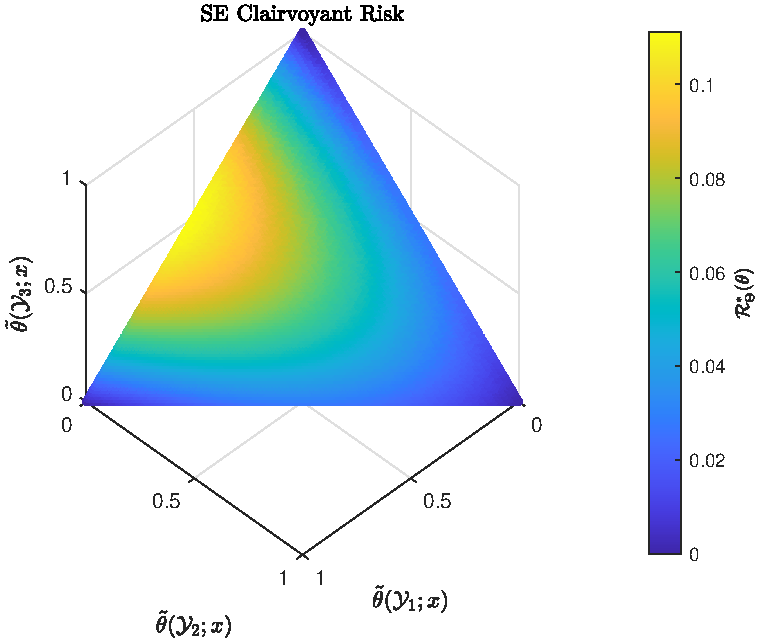
\includegraphics[width=0.7\linewidth]{Risk_clv_SE_tilde.pdf}
\caption{Clairvoyant Risk for the Squared-Error Loss Function, constant $\thetac(x)$}
\label{fig:Risk_clv_SE_tilde}
\end{figure}

\todohi{conditional location?}



\subsubsection{Bayesian Estimation}

\paragraph{Optimal Estimate: the Posterior Mean}

To find the optimal estimator, the squared-error loss is substituted into \eqref{eq:f_opt_xD}. Again, the function over $h$ is positive-definite; as such, the minimizing decision $h$ is the sole stationary point. Setting the first derivative of the function to zero, the optimal estimate is the expected value of $\yrm$ given the training data and the observed value $\xrm$, such that
\begin{IEEEeqnarray}{rCl} \label{eq:f_opt_SE}
f^*(\xrm;\Drm) & = & \argmin_{h \in \Rbb} \Erm_{\yrm | \xrm,\Drm} \left[ (h-\yrm)^2 \right] \\
& = & \mu_{\yrm | \xrm,\Drm} = \Erm_{\uptheta | \xrm,\Drm} \left[ \mu_{\yrm | \xrm,\uptheta} \right] \nonumber \;.
\end{IEEEeqnarray}

An interesting form for the optimal estimator is $f^*(\xrm;\Drm) = \Erm_{\uptheta | \xrm,\Drm} \big[ f_{\Theta}(\xrm;\uptheta) \big]$. Substituting the squared-error loss into the second line of \eqref{eq:f_opt_xD}, the optimal Bayes estimator is the condtional expected value of the clairvoyant estimate with respect to the model posterior distribution.







\paragraph{Minimum Risk: the Expected Posterior Variance}

The Bayes squared-error risk for a general learning function is
\begin{IEEEeqnarray}{rCl} \label{eq:risk_SE}
\Rcal(f) & = & \Erm_{\uptheta} \Bigg[ \Erm_{\Drm | \uptheta} \bigg[ \Erm_{\yrm,\xrm | \uptheta} \Big[ \big( f(\xrm;\Drm)-\yrm \big)^2 \Big] \bigg] \Bigg] \\
& = & \Erm_{\xrm,\Drm} \bigg[ \Erm_{\yrm | \xrm,\Drm} \Big[ \big( f(\xrm;\Drm)-\yrm \big)^2 \Big] \bigg] \nonumber \\
& = & \Erm_{\uptheta}\big[\Rcal_{\Theta}^*(\uptheta)\big] + \Erm_{\xrm,\Drm,\uptheta} \Big[ \big( f(\xrm;\Drm) - \mu_{\yrm | \xrm,\uptheta} \big)^2 \Big] \nonumber \\
& = & \Erm_{\xrm,\Drm} \left[ \Sigma_{\yrm | \xrm,\Drm} \right] + \Erm_{\xrm,\Drm} \Big[ \big( f(\xrm;\Drm) - \mu_{\yrm | \xrm,\Drm} \big)^2 \Big] \nonumber \;.
\end{IEEEeqnarray}

Substituting the optimal estimator \eqref{eq:f_opt_SE} into Equation \eqref{eq:risk_SE}, the minimum Bayes risk is the expected conditional variance
\begin{IEEEeqnarray}{rCl} \label{eq:risk_min_SE}
\Rcal^* & = & \Erm_{\xrm,\Drm} \left[ \Sigma_{\yrm | \xrm,\Drm} \right] \\
& = & \Erm_{\xrm,\uptheta} \left[ \Sigma_{\yrm | \xrm,\uptheta} \right] + \Erm_{\xrm,\Drm} \left[ \Crm_{\uptheta | \xrm,\Drm} \left[ \mu_{\yrm | \xrm,\uptheta} \right] \right] \nonumber \\
& = & \Erm_{\uptheta}\big[\Rcal_{\Theta}^*(\uptheta)\big] + \Erm_{\xrm,\Drm} \Big[ \Crm_{\uptheta | \xrm,\Drm} \big[ f_{\Theta}(\xrm;\uptheta) \big] \Big] \nonumber \;.
\end{IEEEeqnarray}
The first term is the irreducible risk. The second term is the expected variance of the clairvoyant estimate $f_{\Theta}(\xrm;\uptheta) = \mu_{\yrm | \xrm,\uptheta}$ with respect to the model posterior PDF $\prm_{\uptheta | \xrm,\Drm}$






\subsection{Classification: the 0-1 Loss}

In this section, the developed framework is applied to a common machine learning task: classification. In classification problems, the set $\Ycal$ is countable and typically finite. Furthermore, the hypothesis space is usually identical to the unobserved variable space; that is $\Hcal = \Ycal$. The 0-1 loss function is the most widely used for these problems; it is represented as
\begin{equation} \label{eq:loss_01}
\Lcal(h,y) = 1 - \delta[h,y] \;.
\end{equation}
Applying the 0-1 loss, the conditional risk \eqref{eq:risk_cond} for a general classifier is
\begin{IEEEeqnarray}{rCl} \label{eq:risk_cond_01}
\Rcal_{\Theta}(f ; \uptheta) & = & 1 - \Erm_{\Drm | \uptheta} \bigg[ \Erm_{\xrm | \uptheta} \Big[ \Prm_{\yrm | \xrm,\uptheta}\big( f(\xrm;\Drm) | \xrm,\uptheta \big) \Big] \bigg] \;.
% & = & 1 - \sum_{x \in \Xcal} \Erm_{\Drm | \uptheta} \Big[ \uptheta\big( f(x;\Drm),x \big) \Big] \nonumber \\
% & = & 1 - \sum_{x \in \Xcal} \upthetam(x) \Erm_{\Drm | \uptheta} \Big[ \upthetac\big( f(x;\Drm);x \big) \Big] \nonumber \;.
\end{IEEEeqnarray}



\subsubsection{Clairvoyant Hypothesis}

\todomid{decision region figures??}

To find the clairvoyant classifier, the 0-1 loss is substituted into \eqref{eq:f_clv_x}; given an observation $x$, the optimum hypothesis is simply the value $y$ that maximizes the conditional model $\upthetac(x)$,
\begin{IEEEeqnarray}{rCl} \label{eq:f_clv_01}
f_{\Theta}(\xrm;\uptheta) & = & \argmin_{h \in \Ycal} \Erm_{\yrm | \xrm,\uptheta} \left[ 1 - \delta[h,y] \right] \\
& = & \argmax_{h \in \Ycal} \Prm_{\yrm | \xrm,\uptheta}(h | \xrm,\uptheta) \nonumber \\
%& = & \argmax_{y \in \Ycal} \upthetac(y;\xrm) \nonumber \\
& = & \argmax_{y \in \Ycal} \uptheta(y,\xrm) \nonumber \;.
\end{IEEEeqnarray}
Substituting the 0-1 loss and clairvoyant hypothesis into \eqref{eq:risk_clv}, the resulting clairvoyant risk is
\begin{IEEEeqnarray}{rCl}
\Rcal_{\Theta}^*(\uptheta) & = & 1 - \Erm_{\xrm | \uptheta} \Big[ \max_{y \in \Ycal} \Prm_{\yrm | \xrm,\uptheta}(y | \xrm,\uptheta) \Big] \;.
%& = & 1 - \sum_{x \in \Xcal} \upthetam(x) \max_{y \in \Ycal} \upthetac(y;x) \nonumber \\
%& = & 1 - \sum_{x \in \Xcal} \max_{y \in \Ycal} \uptheta(y,x) \nonumber \;.
\end{IEEEeqnarray}

Figure \ref{fig:Risk_clv_01_tilde} displays the clairvoyant risk for predictive models $\thetac(x)$ independent of $x$. Intuitively, the models that are more concentrated lead to lower probability of error.
\begin{figure}
\centering
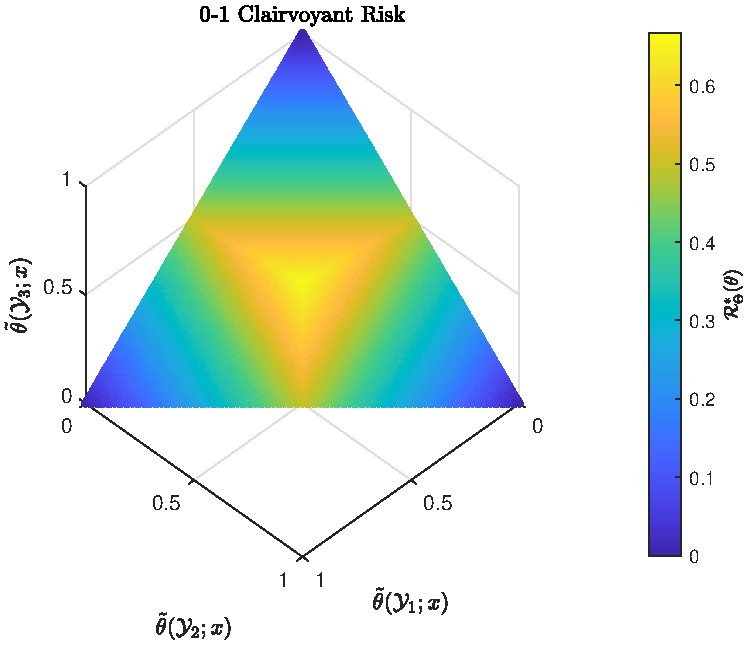
\includegraphics[width=0.7\linewidth]{Risk_clv_01_tilde.pdf}
\caption{Clairvoyant Risk for the 0--1 Loss Function, constant $\thetac(x)$}
\label{fig:Risk_clv_01_tilde}
\end{figure}

\todohi{conditional location?}



\subsubsection{Bayesian Classification}

\paragraph{Optimal Hypothesis: Conditional Maximum \emph{a posteriori}}

To determine the optimal learning function, the 0-1 loss from Equation \eqref{eq:loss_01} is substituted into Equation \eqref{eq:f_opt_xD} to find
\begin{IEEEeqnarray}{rCl} \label{eq:f_opt_01}
f^*(\xrm;\Drm) & = & \argmin_{h \in \Ycal} \Erm_{\yrm | \xrm,\Drm}\big[ 1 - \delta[h,\yrm] \big] \\
& = & \argmax_{y \in \Ycal} \Prm_{\yrm | \xrm,\Drm}(y | \xrm,\Drm) \nonumber \;.
\end{IEEEeqnarray}
The optimal classifier chooses the value $y \in \Ycal$ that maximizes the conditional PMF for the observed values of $\xrm$ and $\Drm$.



\paragraph{Minimum Risk: Probability of Error}

Using the 0-1 loss, the Bayes probability of error \eqref{eq:risk_min} is
\begin{IEEEeqnarray}{rCl} \label{eq:risk_01}
\Rcal(f) & = & 1 - \Erm_{\xrm,\Drm} \left[ \Prm_{\yrm | \xrm,\Drm}\big( f(\xrm;\Drm) | \xrm,\Drm \big) \right] \;.
\end{IEEEeqnarray}

Substituting the optimal learning function \eqref{eq:f_opt_01} into the general risk \eqref{eq:risk_01}, the minimum probability of error is 
\begin{IEEEeqnarray}{rCl} \label{eq:risk_min_01}
\Rcal^* & = & 1 - \Erm_{\xrm,\Drm} \left[ \max_{y \in \Ycal} \Prm_{\yrm | \xrm,\Drm}(y | \xrm,\Drm) \right] \;.
\end{IEEEeqnarray}


















\newpage

\chapter{Discrete-Domain Dirichlet Model}

\todohi{Generalize discussion/math for infinite-countable domains?}

\todohigh{Figs BROKEN from alpha changes}

\todohigh{Uncoupled m/c alphas = non-Dir Ptheta??}

This chapter determines the optimal learning functions when the sets $\Ycal$ and $\Xcal$ have a finite number of elements and the model $\uptheta$ is characterized by a Dirichlet distribution.


\section{Probability Distributions}

To determine the optimal learning function, the joint PMF $\Prm_{\yrm,\xrm,\Drm}$ is required. Having already defined the distribution conditioned on the model $\uptheta$, all that remains is to select a PDF $\prm_{\uptheta}$ reflecting the user's prior knowledge. In this section, the Dirichlet distribution is used. The Dirichlet distribution possesses the desirable property of being the conjugate prior for the multinomial conditional distribution characterizing the data; as such, it will provide analytic forms for the model posterior distribution and lead to closed form expressions for the data conditional distribution used to design the learning function.

Other distributions of interest will be provided, such as the training data PMF $\Prm_{\Drm}$ and the conditional distribution $\Prm_{\yrm | \xrm,\Drm}$ used to form a decision given specific observations.



\subsection{Model PDF, $\prm_{\uptheta}$} \label{sec:P_theta}

The Dirichlet PDF for the model random process $\uptheta \in \Uptheta$ is \cite{bishop}
\begin{IEEEeqnarray}{rCl}
\prm_{\uptheta}(\theta) & = & \beta(\alpha_0 \alpha)^{-1} \prod_{y \in \Ycal} \prod_{x \in \Xcal} \theta(y,x)^{\alpha_0 \alpha(y,x) - 1} \nonumber \\
& = & \Dir\big( \theta ; \alpha_0,\alpha \big) \;,
\end{IEEEeqnarray}
where the user-selected parameterizing distribution $\alpha \in \left\{ {\Rbb^+}^{\Ycal \times \Xcal} : \sum_{y,x} \alpha(y,x) = 1 \right\} \subset \Theta$ and concentration parameter $\alpha_0 \in \Rbb^+$ are introduced. Note that $\beta$ is the generalized beta function.

\todohigh{Use of alpha is REDUNDANT?! Just use mu??}

The first and second joint moments of the model are 
\begin{equation}
\mu_{\uptheta} = \alpha
\end{equation}
and
\begin{IEEEeqnarray}{rCl}
\Erm_{\uptheta}\big[ \uptheta \otimes \uptheta \big] & = & \frac{1}{\alpha_0+1} \diag(\alpha) + \frac{\alpha_0}{\alpha_0+1} \alpha \otimes \alpha \;.
\end{IEEEeqnarray}
%\begin{IEEEeqnarray}{rCl}
%\Erm_{\uptheta}\big[ \uptheta(y,x) \uptheta(y',x') \big] & = & \frac{\alpha(y,x) \delta[y,y'] \delta[x,x'] + \alpha_0 \alpha(y,x) \alpha(y',x')}{\alpha_0+1} \;.
%\end{IEEEeqnarray}
Observe that $\Prm_{\yrm,\xrm}  = \mu_{\uptheta} = \alpha$. The covariance is
\begin{IEEEeqnarray}{rCl}
\Sigma_{\uptheta} & = & \Erm_{\uptheta}\Big[ \big(\uptheta-\mu_{\uptheta}\big) \otimes \big(\uptheta-\mu_{\uptheta}\big) \Big] \\
& = & \frac{\diag(\alpha) - \alpha \otimes \alpha}{\alpha_0+1} \nonumber \;.
\end{IEEEeqnarray}
%\begin{IEEEeqnarray}{rCl}
%\Sigma_{\uptheta}(y,x,y',x') & = & \Erm_{\uptheta}\Big[ \big(\uptheta(y,x)-\mu_{\uptheta}(y,x)\big) \big(\uptheta(y',x')-\mu_{\uptheta}(y',x')\big) \Big] \\
%& = & \frac{\alpha(y,x) \delta[y,y'] \delta[x,x'] - \alpha(y,x) \alpha(y',x')}{\alpha_0+1} \nonumber \;.
%\end{IEEEeqnarray}
Also, for PDF's satisfying $\alpha(y,x) > \alpha_0^{-1}$, the maximizing value of the distribution is
\begin{equation}
\theta_\mathrm{max} = \argmax_{\theta \in \Uptheta} \prm_{\uptheta}(\theta) = \frac{\alpha - \alpha_0^{-1}}{1 - \alpha_0^{-1} |\Ycal||\Xcal|} \;.
\end{equation}
This can be easily shown by maximizing the logarithm of the distribution using the method of Lagrange multipliers.

\todomid{Reference? Mode proof for all values of alpha?}

\todohigh{HALDANE PRIOR}

Of specific interest is how $\prm_{\uptheta}$ changes as the concentration parameter approaches its limiting values. For $\alpha_0 \to \infty$, the PDF concentrates at its mean, resulting in
\begin{IEEEeqnarray}{rCl}
\prm_{\uptheta}(\theta) & \to & \delta\left( \theta - \alpha \right) \;.
\end{IEEEeqnarray}
Conversely, for $\alpha_0 \to 0$, the PDF tends toward
\begin{IEEEeqnarray}{rCl}
\prm_{\uptheta}(\theta) & \to & \sum_{y \in \Ycal} \sum_{x \in \Xcal} \alpha(y,x) \delta\big( \theta - \delta[\cdot,y] \delta[\cdot,x] \big) \;,
\end{IEEEeqnarray}
which distributes its weight among the $|\Ycal| |\Xcal|$ models with an $\ell_0$ norm satisfying $\| \theta \|_0 = 1$. Note that the Dirac delta for these formulas is defined on the set $\Uptheta$, such that $\int_{\Uptheta} \delta(\theta) {\drm}\theta = 1$.

\todohi{formal proof for limiting PDFs??? stirling/gautschi?}

These trends are demonstrated with Figure \ref{fig:P_theta}. The cardinalities $|\Ycal| = 3$ and $|\Xcal| = 1$ are chosen to enable visualization, despite the implication that $\xrm$ is deterministic; these cardinalities will be used for many subsequent figures as well. Note that for $\alpha_0=2.99 < |\Ycal||\Xcal|$, the PDF values at the boundaries of the domain tend to infinity; this is not captured by the plot color scale.

\begin{figure}
\centering
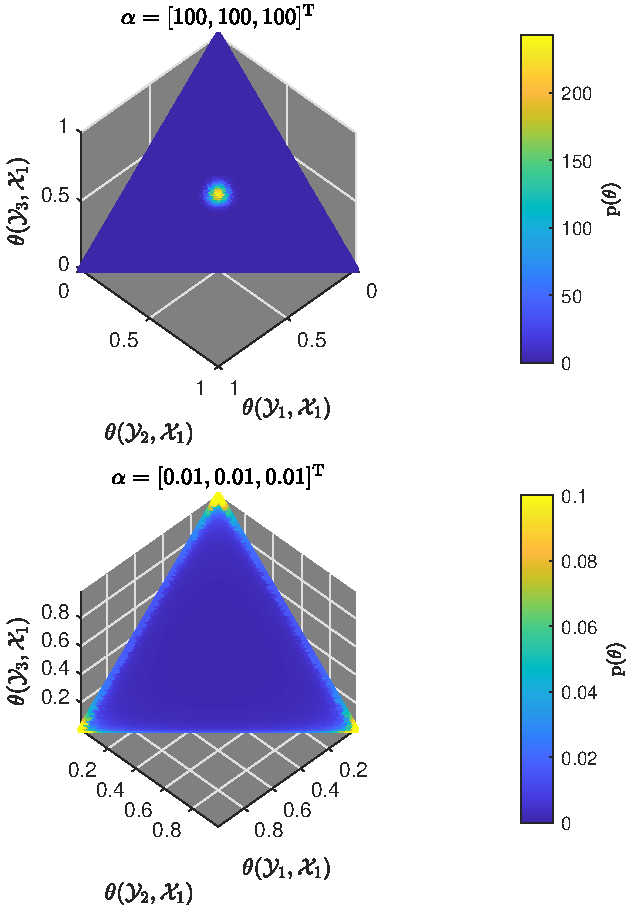
\includegraphics[width=0.7\linewidth]{P_theta.pdf}
\caption{Model prior PDF for different concentrations $\alpha_0$}
\label{fig:P_theta}
\end{figure}





\paragraph{Uniform Prior}

When the Dirichlet parameters are $\alpha(y,x) = \big( |\Ycal||\Xcal| \big)^{-1}$ and $\alpha_0 = |\Ycal||\Xcal|$, the distribution becomes a uniform PDF and is represented as
\begin{equation}
\prm_{\uptheta} = \big( |\Ycal||\Xcal|-1 \big)! \;.
\end{equation}




\subsubsection{Marginal and Conditional Distributions}

PGR: move/add Dir figs here? 

The marginal distribution $\upthetam$ and the conditional distribution $\upthetac$ are also of interest. For brevity, introduce the bijection $\alpha \Leftrightarrow (\alpham,\alphac)$, where $\alpham \equiv \sum_{y \in \Ycal} \alpha(y,\cdot)$, and $\alphac(x) \equiv \alpha(\cdot,x) / \alpham(x)$ for each $x \in \Xcal$. Observe that $\alpham \in \Pcal(\Xcal)$ and $\alphac \in \Pcal(\Ycal)^{\Xcal}$.


By the aggregation property \cite{ferguson}, $\upthetam \sim \Dir(\alpha_0,\alpham)$ is a Dirichlet random process parameterized by concentration $\alpha_0$ and distribution $\alpham$; observe that $\Prm_{\xrm} = \mu_{\upthetam} = \alpham$. Also of interest is the distribution of the predictive model $\upthetac$ conditioned on the marginal $\upthetam$. As demonstrated in Appendix \ref{app:Dir_agg}, these random processes are jointly distributed as
\begin{IEEEeqnarray}{rCl}
\prm_{\upthetac | \upthetam}(\thetac | \thetam) & = & \prm_{\upthetac}(\thetac) \\
& = & \prod_{x \in \Xcal} \Bigg[ \beta\big( \alpha_0 \alpham(x) \alphac(x) \big)^{-1} \prod_{y \in \Ycal} \thetac(y;x)^{\alpha_0 \alpham(x) \alphac(y;x) - 1} \Bigg] \nonumber \\
& = & \prod_{x \in \Xcal} \Dir\Big( \thetac(x) ; \alpha_0 \alpham(x), \alphac(x) \Big) \nonumber \;,
\end{IEEEeqnarray}
\begin{IEEEeqnarray}{rCl}
\upthetac | \upthetam & \sim & \upthetac \sim \bigotimes_{x \in \Xcal} \Dir\Big( \alpha_0 \alpham(x), \alphac(x) \Big) \;,
\end{IEEEeqnarray}
a product of Dirichlet distributions defined on $\thetac \in \Pcal(\Ycal)^{\Xcal}$. As shown, the processes $\upthetac(x)$ are Dirichlet with parameterizing distributions $\alphac(x)$ and concentrations $\alpha_0 \alpham(x)$, independent of one another, and independent of the marginal distribution $\upthetam$. Note that $\Prm_{\yrm | \xrm} = \mu_{\upthetac}(\xrm) = \alphac(\xrm)$. 









\begin{figure}
\centering
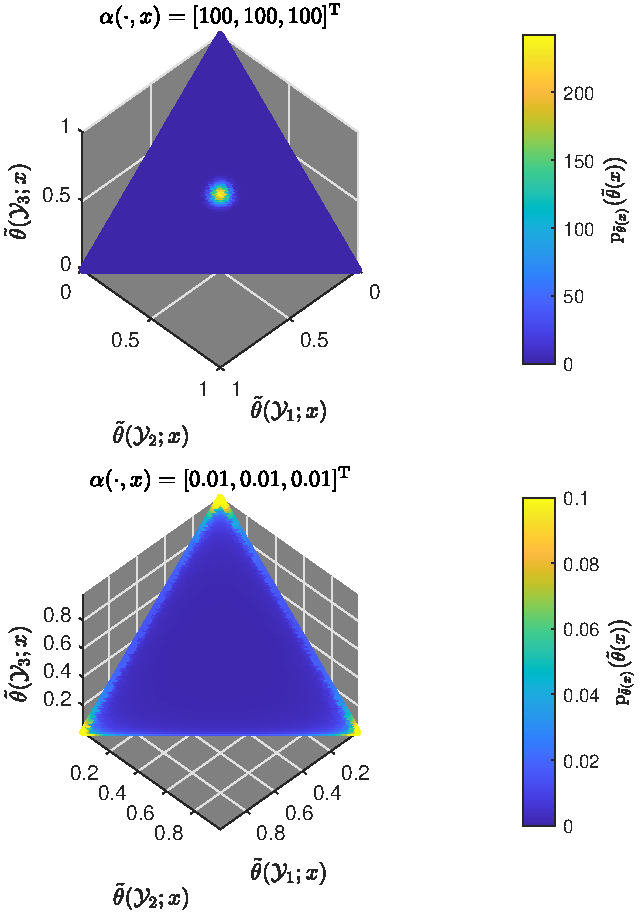
\includegraphics[width=0.7\linewidth]{P_theta_tilde.pdf}
\caption{Model prior PDF for different concentrations $\alpha_0 \alpham(x)$}
%\label{fig:P_theta}
\end{figure}






\subsection{Training Set PMF, $\Prm_{\Drm}$}

\todolo{EVIDENCE TERMINOLOGY??}

Next, the conditional distribution $\Prm_{\Drm | \uptheta}$ will be used to determine the marginal PMF, $\Prm_{\Drm}$ and properties will be discussed.


As the conditional distribution $\Prm_{\Drm | \uptheta}$ is of exponential form, it can be readily shown that the marginal distribution of the training data is \cite{minka-multi}
\begin{IEEEeqnarray}{rCl}
\Prm_{\Drm}(D) & = & \Erm_{\uptheta} \left[ \prod_{n=1}^N \Prm_{\Drm_n | \uptheta}\big( D_n | \uptheta \big) \right] \\
& = & \Erm_{\uptheta} \left[ \left( \prod_{y \in \Ycal} \prod_{x \in \Xcal} \uptheta(y,x)^{\Psi(y,x;D)} \right)^N \right] \nonumber \\
& = & \frac{\beta\big( \alpha_0 \alpha + N \Psi(D) \big)}{\beta(\alpha_0 \alpha)} \nonumber \;.
\end{IEEEeqnarray}
Note that values of the PMF $\Prm_{\Drm}$ are equivalent to joint moments of the model $\uptheta$. 

It is instructive to consider the limiting forms of this distribution for the extreme values of the model concentration parameter $\alpha_0$. As $\alpha_0 \to \infty$, the model concetrates at its mean and the training data $\Drm$ distribution is
\begin{IEEEeqnarray}{rCl}
\Prm_{\Drm}(D) & \to & \Erm_{\uptheta}\left[ \prod_{n=1}^N \uptheta(Y_n,X_n) \right] \\
& = & \prod_{n=1}^N \alpha\big( Y_n,X_n \big) \nonumber \;.
\end{IEEEeqnarray}
Conversely, as $\alpha_0 \to 0$, the distribution becomes
\begin{IEEEeqnarray}{rCl}
\Prm_{\Drm}(D) & \to & \sum_{y \in \Ycal} \sum_{x \in \Xcal} \alpha(y,x) \prod_{n=1}^N \delta\big[ D_n,(y,x) \big] 
\end{IEEEeqnarray}
and the training data are identical.



Next, the distribution of the sufficient statistic $\uppsi$ will be represented. As a Dirichlet distribution characterizes the parameters of the Empirical distribution $\Prm_{\uppsim | \uptheta}$, the PMF of $\uppsi$ is a Dirichlet-Empirical distribution (related to the Dirichlet-Multinomial distribution \cite{johnson}) for $N$ samples, concentration $\alpha_0$, and parameter distribution $\alpha$, such that
\begin{IEEEeqnarray}{rCl}
\Prm_{\uppsi}(\psi) & = & \Mcal(N \psi) \frac{\beta(\alpha_0 \alpha + N \psi)}{\beta(\alpha_0 \alpha)} \\
& = & \DE\big( \psi; N,\alpha_0, \alpha \big) \nonumber \;.
\end{IEEEeqnarray}

The first and second joint moments of the empirical model $\uppsi$ are
\begin{IEEEeqnarray}{rCl}
\mu_{\uppsi} & = & \alpha = \mu_\uptheta 
\end{IEEEeqnarray}
and
\begin{IEEEeqnarray}{L}
\Erm_{\uppsi}\big[ \uppsi \otimes \uppsi \big] = \frac{\alpha_0^{-1} + N^{-1}}{1 + \alpha_0^{-1}} \diag(\alpha) + \frac{1 - N^{-1}}{1 + \alpha_0^{-1}} \alpha \otimes \alpha \nonumber \;.
\end{IEEEeqnarray}
%\begin{IEEEeqnarray}{L}
%\Erm_{\uppsi}\big[ \uppsi(y,x) \uppsi(y',x') \big] \\
%\qquad = \frac{1}{1 + \alpha_0^{-1}} \Big( (\alpha_0^{-1} + N^{-1}) \alpha(y,x) \delta[y,y'] \delta[x,x'] + (1 - N^{-1}) \alpha(y,x) \alpha(y',x') \Big) \nonumber \;.
%\end{IEEEeqnarray}
The covariance function is
\begin{IEEEeqnarray}{rCl}
\Sigma_{\uppsi} & = & \frac{\alpha_0^{-1} + N^{-1}}{1 + \alpha_0^{-1}} \big( \diag(\alpha) - \alpha \otimes \alpha \big) \\
& = & \left(1 + \frac{\alpha_0}{N}\right) \Sigma_{\uptheta} \nonumber \;.
\end{IEEEeqnarray}
%\begin{IEEEeqnarray}{rCl}
%\Sigma_{\uppsi}(y,x,y',x') & = & \frac{\alpha_0^{-1} + N^{-1}}{1 + \alpha_0^{-1}} \big( \alpha(y,x) \delta[y,y'] \delta[x,x'] - \alpha(y,x) \alpha(y',x') \big) \\
%& = & \left(1 + \frac{\alpha_0}{N}\right) \Sigma_{\uptheta}(y,x,y',x') \nonumber \;.
%\end{IEEEeqnarray}
Observe that as $N \to \infty$, the variance $\Sigma_{\uppsi} \to \Sigma_{\uptheta}$.


Observe that as the number of training samples increases, the statistic PMF tends toward $\Prm_{\uppsi}(\psi) \approx N^{1-|\Ycal||\Xcal|}\prm_{\uptheta}(\psi)$; this can be proven using Gautschi's inequality \cite{wendel}. Figure \ref{fig:P_nbar_N} shows how a specific model prior influences the data PMF differently for different $N$.
\begin{figure}
\centering
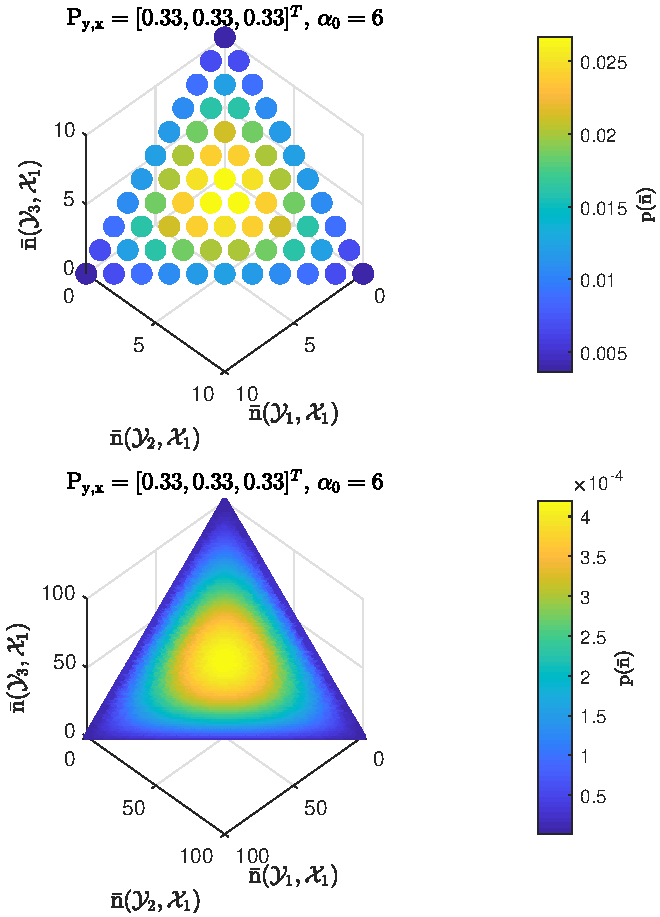
\includegraphics[width=0.7\linewidth]{P_nbar_N.pdf}
\caption{$\Prm_{\uppsi}$ for different training set sizes $N$}
\label{fig:P_nbar_N}
\end{figure}



Again, the data PMF's for minimal and maximal concentration $\alpha_0$ are relevant. For $\alpha_0 \to \infty$, the model PDF $\prm_{\uptheta}$ concentrates at its mean, $\alpha$, and thus $\uppsi$ is characterized by an Empirical distribution,
\begin{IEEEeqnarray}{rCl}
\Prm_{\uppsi}(\psi) & \to & \Mcal(N \psi) \left( \prod_{y \in \Ycal} \prod_{x \in \Xcal} \alpha(y,x)^{\psi(y,x)} \right)^N
\end{IEEEeqnarray}
Conversely, for $\alpha_0 \to 0$, the PMF tends toward
\begin{IEEEeqnarray}{rCl} \label{eq:P_n_lim_zero}
\Prm_{\uppsi}(\psi) & \to & \sum_{y \in \Ycal} \sum_{x \in \Xcal} \alpha(y,x) \delta\big[ \psi , \delta[\cdot,y] \delta[\cdot,x] \big] \;.
\end{IEEEeqnarray}

\todohi{formal proofs for limiting PMFs? stirling/gautschi?}

Figure \ref{fig:P_nbar_a0} displays example distributions of $\uppsi$ for $N=10$ and different model concentrations $\alpha_0$. Observe that for large $\alpha_0$, the distribution approaches an Empirical distribution $\uppsi \sim \Emp(N,\alpha)$. 

\begin{figure}
\centering
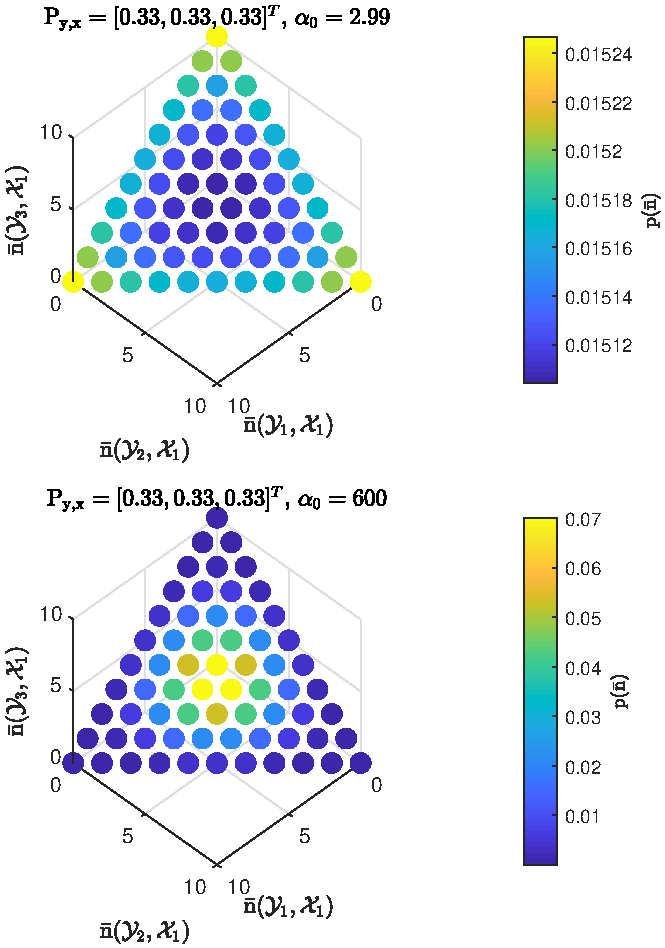
\includegraphics[width=0.7\linewidth]{P_nbar_a0.pdf}
\caption{$\Prm_{\uppsi}$ for different prior concentrations $\alpha_0$}
\label{fig:P_nbar_a0}
\end{figure}





\paragraph{Uniform Prior}

For the uniform prior distribution, $\alpha(y,x) = \big( |\Ycal||\Xcal| \big)^{-1}$ and $\alpha_0 = |\Ycal||\Xcal|$,
\begin{IEEEeqnarray}{rCl} 
\Prm_{\Drm}(D) & = & \Mcal\big( (N,|\Ycal||\Xcal|-1) \big)^{-1} \Mcal\big( N \Psi(D) \big)^{-1}
\end{IEEEeqnarray}
and
\begin{IEEEeqnarray}{rCl}
\Prm_{\uppsi} & = & |\Uppsi|^{-1} = \Mcal\big( (N,|\Ycal||\Xcal|-1) \big)^{-1} \;.
\end{IEEEeqnarray}
The distribution of $\uppsi$ is uniform over the set $\Uppsi$. The PMF for $\Drm$ depends on the training data only through the multinomial coefficient; consequently, more ``concentrated''  training sets are more probable.




\subsubsection{Marginal and Conditional Distributions}

It is also useful to express the marginal and conditional distributions for the training data given the Dirichlet prior. As $\Prm_{\Xrm | \uptheta}$ is of exponential form with respect to the marginal model $\upthetam$, the marginal distribution of $\Xrm$ can be expressed as 
\begin{IEEEeqnarray}{rCl}
\Prm_{\Xrm}(X) & = & \Erm_{\upthetam} \big[ \Prm_{\Xrm | \upthetam} \big](X) \\
& = & \Erm_{\uptheta} \left[ \prod_{n=1}^N \Prm_{\Xrm_n | \uptheta}\big( X_n | \uptheta \big) \right] \nonumber \\
& = & \Erm_{\upthetam} \left[ \left( \prod_{x \in \Xcal} \upthetam(x)^{\Psim(x;X)} \right)^N \right] \nonumber \\
& = & \frac{\beta\big( \alpha_0 \alpham + N \Psim(X) \big)}{\beta(\alpha_0 \alpham)} \nonumber \;.
\end{IEEEeqnarray}
As the model marginal $\upthetam$ and conditional $\upthetac$ are independent, the distribution $\Prm_{\Yrm | \Xrm}$ can be represented as
\begin{IEEEeqnarray}{rCl}
\Prm_{\Yrm | \Xrm}(Y | X) & = & \Erm_{\upthetac}\big[ \Prm_{\Yrm | \Xrm,\upthetac} \big](Y ; X) \\
& = & \prod_{x \in \Xcal} \Erm_{\upthetac(x)}\left[ \prod_{y \in \Ycal} \upthetac(y;x)^{N \Psim(x;X) \Psic(y;x;Y,X)} \right] \nonumber \\
& = & \prod_{x \in \Xcal} \frac{\beta\big( \alpha_0 \alpham(x) \alphac(x) + N \Psim(x;X) \Psic(x;Y,X) \big)}{\beta\big( \alpha_0 \alpham(x) \alphac(x) \big)} \nonumber \;.
\end{IEEEeqnarray}



The corresponding distributions for the sufficient statistics will be expressed as well. Recall that $\uppsim | \uptheta \sim \Emp(N,\upthetam)$; by the aggregation property of Dirichlet-Empirical functions (inherited from the Dirichlet-Multinomial properties \cite{johnson}), the random process is distributed as $\uppsim \sim \DE(N,\alpha_0,\alpham)$.

Also of interest is the distribution of $\uppsic$ conditioned on its aggregation $\uppsim$. Using the Dirichlet-Empirical properties presented in Appendix \ref{app:DE}, it can be shown that
\begin{IEEEeqnarray}{rCl}
\Prm_{\uppsic | \uppsim}(\psic | \psim) & = & \prod_{x \in \Xcal} \left[ \Mcal\big( N \psim(x) \psic(x) \big) \frac{\beta\big( \alpha_0 \alpham(x) \alphac(x) + N \psim(x) \psic(x) \big)}{\beta\big( \alpha_0 \alpham(x) \alphac(x) \big)} \right] \\
& = & \prod_{x \in \Xcal} \DE\Big( \psic(x) ; N \psim(x), \alpha_0 \alpham(x), \alphac(x) \Big) \nonumber
\end{IEEEeqnarray}
over the domain $\prod_{x \in \Xcal} \left\{ \frac{n}{N \psim(x)}: n \in {\Zbbgeq}^{\Ycal} : \sum_{y \in \Ycal} n(y) = N \psim(x) \right\}$. Observe that conditioning on the marginal empirical process renders the conditional processes $\uppsic(x)$ independent of one another and that they are also Dirichlet-Empirical, such that $\uppsic(x) | \uppsim(x) \sim \DE\big( N \uppsim(x),\alpha_0 \alpham(x), \alphac(x) \big)$.












\subsection{Predictive PMF, $\Prm_{\yrm | \xrm,\Drm}$}

As shown in Equation \eqref{eq:f_opt_xD}, the decision selected by the optimally designed function depends on $\Prm_{\yrm | \xrm,\Drm}$, the distribution of the unobserved $\yrm$ conditioned on all observable random elements. This PMF will be expressed next.

First observe that since $\Prm_{\Drm | \uptheta}$ is of exponential form, the Dirichlet prior $\prm_{\uptheta}$ is its conjugate prior \cite{theodoridis-ML}; thus, the model posterior PDF given the training data is
\begin{IEEEeqnarray}{rCl}
\prm_{\uptheta | \Drm}(\theta | D) & = & \beta \left( \alpha_0 \alpha + N \Psi(D) \right)^{-1} \prod_{y \in \Ycal} \prod_{x \in \Xcal} \theta(y,x)^{\alpha_0 \alpha(y,x) + N \Psi(y,x;D) - 1} \;, 
\end{IEEEeqnarray}
a Dirichlet distribution with concentration $\alpha_0 + N$ and parameter distribution 
\begin{IEEEeqnarray}{rCl}
\mu_{\uptheta | \Drm} & = & \frac{\alpha_0 \alpha + N \Psi(\Drm)}{\alpha_0 + N} \\
& = & \gamma \alpha + (1 - \gamma) \Psi(\Drm) \nonumber \;,
\end{IEEEeqnarray}
where the weight
\begin{IEEEeqnarray}{L}
\gamma = \left(1 + \frac{N}{\alpha_0}\right)^{-1} \in (0, 1]
\end{IEEEeqnarray}
is introduced.

\todolo{Comment on N=0 case, psi not a valid PF?}

This posterior distribution is of specific interest in the machine learning literature. While Bayesian techniques are used here, often point estimates of the model $\uptheta$ are formed; perhaps the most common approach is to form the Maximum a posteriori estimate,
\begin{IEEEeqnarray}{rCl}
\theta_\mathrm{MAP}(D) & = & \argmax_{\theta \in \Uptheta} \Prm_{\uptheta | \Drm}(\theta | D) = \frac{\alpha_0 \alpha + N \Psi(D) - 1}{\alpha_0 + N - |\Ycal||\Xcal|} \\
& = & \frac{\alpha_0}{\alpha_0 - |\Ycal||\Xcal| + N} (\alpha - \alpha_0^{-1}) + \frac{N}{\alpha_0 - |\Ycal||\Xcal| + N} \Psi(\Drm) \nonumber \;.
\end{IEEEeqnarray}
This maximizing value is only valid if $\mu_{\uptheta | \Drm} > (\alpha_0 + N)^{-1}$. For the uniform model prior, the maximizing value of the posterior is the empirical model $\Psi(D)$.

\todolow{MAP discussion out of place?}

Observe that the concentration parameter increases proportionately with both the training data volume and the prior concentration. Consequently, as $N \to \infty$, $\gamma \to 0$ and the posterior converges to $\prm_{\uptheta | \Drm} \to \delta\big( \cdot - \Psi(\Drm) \big)$; as more data is collected, the model can be more positively identified and used to formulate minimum risk decisions. Conversely, as $\alpha_0 \to \infty$, $\gamma \to 1$ reflection confidence in the prior and the posterior tends toward $\prm_{\uptheta | \Drm} \to \delta( \cdot - \alpha)$, independent of the training data.

Figure \ref{fig:P_theta_D} shows the influence of the training data on the model distribution; after conditioning on the training data (via $\uppsi$), the PDF concentration shifts away from the models favored by the prior knowledge and towards other models that better account for the observations.

\begin{figure}
\centering
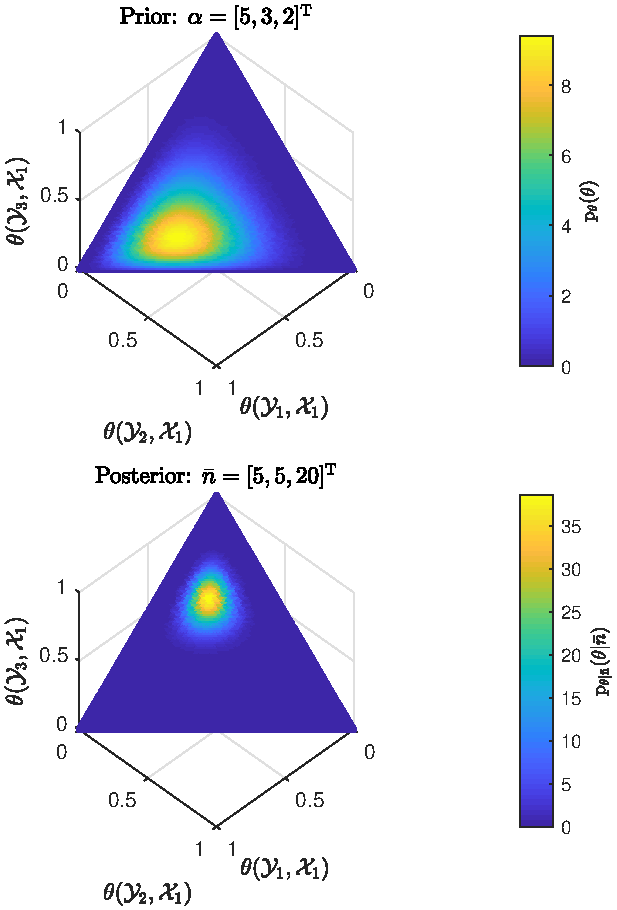
\includegraphics[width=0.7\linewidth]{P_theta_post.pdf}
\caption{Model $\uptheta$ PDF, prior and posterior}
\label{fig:P_theta_D}
\end{figure}


Recall that the joint PMF of $\yrm$ and $\xrm$ conditioned on the training data is equivalent to the posterior mean $\mu_{\uptheta | \Drm}$, such that \cite{murphy}
\begin{IEEEeqnarray}{rCl}
\Prm_{\yrm,\xrm | \Drm} & = & \gamma \alpha + (1-\gamma) \Psi(\Drm) \;.
\end{IEEEeqnarray}
This is a mixture distribution of the prior mean $\mu_{\uptheta} = \alpha$ and the empirical distribution $\Psi(\Drm)$. The more informative the model prior (i.e. larger $\alpha_0$), the more the prior mean is favored; the more data, the more the empirical model is favored. The marginal distribution for $\xrm$ given $\Drm$ is
\begin{IEEEeqnarray}{rCl}
\Prm_{\xrm | \Drm} \equiv \Prm_{\xrm | \Xrm} & = & \frac{\alpha_0 \alpham + N \Psim(\Xrm)}{\alpha_0 + N} \nonumber \\
& = & \gamma \alpham + (1-\gamma) \Psim(\Xrm) \;.
\end{IEEEeqnarray}

Finally, the predictive distribution of interest is generated via Bayes rule as
\begin{IEEEeqnarray}{rCl} \label{eq:P_y_xD_dir}
\Prm_{\yrm | \xrm,\Drm} & = & \frac{\alpha_0 \alpha(\cdot,\xrm) + N \Psi(\cdot,\xrm;\Drm)}{\alpha_0 \alpham(\xrm) + N \Psim(\xrm;\Drm)} \\
& = & \left(\frac{\alpha_0 \alpham(\xrm)}{\alpha_0 \alpham(\xrm) + N \Psim(\xrm;\Drm)}\right) \alphac(\xrm) + \left(\frac{N \Psim(\xrm;\Drm)}{\alpha_0 \alpham(\xrm) + N \Psim(\xrm;\Drm)}\right) \Psic(\xrm;\Drm) \nonumber \\
& \equiv & \gammam(\xrm;\Xrm) \alphac(\xrm) + \big(1 - \gammam(\xrm;\Xrm)\big) \Psic(\xrm;\Drm) \nonumber \;,
\end{IEEEeqnarray}
where the ``marginal'' weighting function
\begin{IEEEeqnarray}{L}
\gammam(X) = \left(1 + \frac{N \Psim(X)}{\alpha_0 \alpham}\right)^{-1} \in (0, 1]^{\Xcal}
\end{IEEEeqnarray}
is introduced. The last representation views the distribution as a convex combination of two conditional distributions. The first distribution $\Prm_{\yrm | \xrm} = \alphac(\xrm)$ is independent of the training data and based on the prior knowledge implied via the model PDF parameter; the second distribution is the conditional empirical model and depends on $\Drm$, not on $\alpha$.

Recall that the weighting factors $\alpha_0 \alpham(x)$ and $N \Psim(x;\Drm)$ are the concentration of the conditional prior $\upthetac(x)$ and the number of training samples characterizing the conditional empirical model $\uppsic(x)$ (samples satisfying $X_n = \xrm$), respectively. As the former increases relative to the latter, the weight value $\gammam(x; \Xrm) \to 0$ and $\Prm_{\yrm | \xrm,\Drm}$ tends away from the prior function $\alphac(x)$ and towards the empirical conditional distribution $\Psic(x;\Drm)$.


\paragraph{Uniform Prior}

For the uniform model prior PDF, the conditional distribution is
\begin{IEEEeqnarray}{rCl} \label{eq:P_y_xD_dir_uni}
\Prm_{\yrm | \xrm,\Drm} & = & \frac{N \Psi(\cdot,\xrm;\Drm)+1}{N \Psim(\xrm;\Drm) + |\Ycal|} \\
& = & \left(\frac{|\Ycal|}{|\Ycal| + N \Psim(\xrm;\Drm)}\right) \frac{1}{|\Ycal|} + \left(\frac{N \Psim(\xrm;\Drm)}{|\Ycal| + N \Psim(\xrm;\Drm)}\right) \Psic(\xrm;\Drm) \nonumber \;.
\end{IEEEeqnarray}
Now the prior PMF contribution $\alphac(x)$ is a uniform distribution over the $|\Ycal|$ possible outputs. The weighting factors are dependent on conditional prior concentration $\alpha_0 \alpham(\xrm) = |\Ycal|$; the more possible outcomes $|\Ycal|$ there are for a given training set size, the more the Bayesian predictive distribution tends toward the uniform PMF.



\subsubsection{Via the Conditional Model Distribution}

PGR: reference posterior equations!

PGR: DIR FIGS? for PDF asymptotics?


The Bayesian distributions $\Prm_{\xrm | \Drm}$ and $\Prm_{\yrm | \xrm,\Drm}$ can also be found from the posterior distributions $\prm_{\upthetam | \Drm}$ and $\prm_{\upthetac | \xrm,\Drm}$, respectively. As the Dirichlet assumption renders $\upthetam$ and $\upthetac$ independent, it can be shown that $\Prm_{\Yrm | \Xrm} = \Erm_{\upthetac}\big[ \Prm_{\Yrm | \Xrm,\upthetac} \big]$ and thus that $\upthetam$ is conditionally independent of $\Yrm$ given $\Xrm$. Furthermore, the Dirichlet distribution $\prm_{\upthetam}$ is a conjugate prior for the likelihood $\Prm_{\Xrm | \upthetam}$. As a result, $\upthetam | \Drm \sim \Dir\big (\alpha_0 + N, \mu_{\upthetam | \Xrm} \big)$ and
\begin{IEEEeqnarray}{rCl}
\Prm_{\xrm | \Drm} & = & \mu_{\upthetam | \Drm} \\
& \equiv & \mu_{\upthetam | \Xrm} = \gamma \alpham + (1-\gamma) \Psim(\Xrm) \nonumber \;.
\end{IEEEeqnarray}
Similarly, the distribution can be expressed in terms of the empirical model sufficient statistic as
\begin{IEEEeqnarray}{rCl}
\Prm_{\xrm | \uppsi} & = & \mu_{\upthetam | \uppsi} \\
& \equiv & \mu_{\upthetam | \uppsim} = \gamma \alpham + (1-\gamma) \uppsim \nonumber \;,
\end{IEEEeqnarray}
where the dependency on $\uppsi$ is expressed only through the marginal random process $\uppsim$.

\todomid{independence of conditionals too}

The posterior $\prm_{\upthetac | \xrm,\Drm}$ can be simplified by noting that the independence of $\upthetam$ and $\upthetac$ implies $\Prm_{\Yrm | \Xrm,\xrm} = \Erm_{\upthetac}\big[ \Prm_{\Yrm | \Xrm,\upthetac} \big] = \Prm_{\Yrm | \Xrm}$. Consequently, $\upthetac$ is conditionally independent of $\xrm$ given $\Drm$. Thus, as $\prm_{\upthetac}$ is a conjugate prior for $\Prm_{\Yrm | \Xrm,\upthetac}$ the posterior distribution is
\begin{IEEEeqnarray}{rCl}
\prm_{\upthetac | \xrm,\Drm}(\thetac | x,D) & = & \prm_{\upthetac | \Drm}(\thetac | D) = \prod_{x' \in \Xcal} \prm_{\upthetac(x') | \Drm}\big(\thetac(x') | D \big) \\
& = & \prod_{x' \in \Xcal} \Dir\big( \thetac(x') ; \alpha_0 \alpham(x') + N \Psim(x';D), \mu_{\upthetac | \Drm}(x'; D) \big) \nonumber \;,
\end{IEEEeqnarray}
\begin{IEEEeqnarray}{rCl}
\prm_{\upthetac | \xrm,\Drm} & = & \prm_{\upthetac | \Drm} = \prod_{x' \in \Xcal} \prm_{\upthetac(x') | \Drm} \\
& = & \prod_{x' \in \Xcal} \Dir\big( \alpha_0 \alpham(x') + N \Psim(x';\Drm), \mu_{\upthetac(x') | \Drm} \big) \nonumber \;,
\end{IEEEeqnarray}
where
\begin{IEEEeqnarray}{rCl}
\mu_{\upthetac | \xrm,\Drm}(x'; x,D) & = & \mu_{\upthetac | \Drm}(x'; D) \\
& \equiv & \gammam(x';X) \alphac(x') + \big(1 - \gammam(x';X)\big) \Psic(x';D) \nonumber
\end{IEEEeqnarray} 
\begin{IEEEeqnarray}{rCl}
\mu_{\upthetac | \xrm,\Drm} & = & \mu_{\upthetac | \Drm} = \bigotimes_{x' \in \Xcal} \mu_{\upthetac(x') | \Drm}  \\
& \equiv & \bigotimes_{x' \in \Xcal} \left( \gammam(x';X) \alphac(x') + \big(1 - \gammam(x';\Xrm)\big) \Psic(x';\Drm) \right) \nonumber
\end{IEEEeqnarray} 
and the distinct model conditional PMF's are independent from one another. The Bayes predictive PMF can thus be expressed as
\begin{IEEEeqnarray}{rCl}
\Prm_{\yrm | \xrm,\Drm}(x,\Drm) & = & \mu_{\upthetac(x) | \xrm,\Drm}(x,\Drm) = \mu_{\upthetac(x) | \Drm} \;.
\end{IEEEeqnarray}

A similar treatment demonstrates that
\begin{IEEEeqnarray}{rCl}
\prm_{\upthetac | \xrm,\uppsi}( \thetac | x,\psi ) & = & \prm_{\upthetac | \uppsi}( \thetac | \psi ) \equiv \prm_{\upthetac | \uppsim, \uppsic}( \thetac | \psim, \psic ) \\
& = & \prod_{x' \in \Xcal} \prm_{\upthetac(x') | \uppsim(x'), \uppsic(x')}\big(\thetac(x') | \psim(x'), \psic(x') \big) \nonumber \\
& = & \prod_{x' \in \Xcal} \Dir\Big( \thetac(x') ; \alpha_0 \alpham(x') + N \psim(x'), \mu_{\upthetac(x') | \uppsim(x'), \uppsic(x')}\big( \psim(x'), \psic(x') \big) \Big) \nonumber \;,
\end{IEEEeqnarray}
\begin{IEEEeqnarray}{rCl}
\prm_{\upthetac | \xrm,\uppsi} & = & \prm_{\upthetac | \uppsi} \equiv \prm_{\upthetac | \uppsim, \uppsic} \\
& = & \bigotimes_{x' \in \Xcal} \prm_{\upthetac(x') | \uppsim(x'), \uppsic(x')} \nonumber \\
& = & \bigotimes_{x' \in \Xcal} \Dir\Big(\alpha_0 \alpham(x') + N \uppsim(x'), \mu_{\upthetac(x') | \uppsim(x'), \uppsic(x')} \Big) \nonumber \;,
\end{IEEEeqnarray}

where
\begin{IEEEeqnarray}{L}
\mu_{\upthetac(x') | \uppsim(x'), \uppsic(x')} = \gammam(x'; \uppsim) \alphac(x') + \big(1 - \gammam(x'; \uppsim) \big) \uppsic(x') \nonumber \;.
\end{IEEEeqnarray}
\begin{IEEEeqnarray}{rCl}
\mu_{\upthetac | \uppsim, \uppsic} & = & \bigotimes_{x' \in \Xcal} \mu_{\upthetac(x') | \uppsim(x'), \uppsic(x')} \\
& = & \bigotimes_{x' \in \Xcal} \left( \gammam(x'; \uppsim) \alphac(x') + \big(1 - \gammam(x'; \uppsim) \big) \uppsic(x') \right) \nonumber \;.
\end{IEEEeqnarray}
and the modified weighting function
\begin{IEEEeqnarray}{L}
\gammam(\psim) = \left(1 + \frac{N \psim}{\alpha_0 \alpham}\right)^{-1} \in (0, 1]^{\Xcal}
\end{IEEEeqnarray}
is introduced, operating on the empirical data distribution.

\todohi{Reconcile different weighting funcs for D and psi...}

Observe that when the conditioning is performed using the sufficient statistic, the independent conditional models $\upthetac(x)$ are only dependent on the marginal empirical model value $\uppsim(x)$ and on the corresponding conditional empirical model, $\uppsic(x)$. 

The Bayes predictive PMF can thus be expressed as 
\begin{IEEEeqnarray}{rCl}
\Prm_{\yrm | \xrm,\uppsi}(x,\uppsi) = \mu_{\upthetac(x) | \xrm,\uppsi}(x,\uppsi) & \equiv & \mu_{\upthetac(x) | \uppsim(x), \uppsic(x)} \nonumber \;.
\end{IEEEeqnarray}
%A consequence of the Dirichlet prior is that the predictive PMF for a given value of $\xrm$ only depends on the corresponding training data $\uppsi(\cdot,\xrm)$, such that $\Prm_{\yrm | \xrm,\uppsi}(x,\psi) = \Prm_{\yrm | \xrm,\uppsi(\cdot,\xrm)}\big( x,\psi(\cdot,x) \big)$. This is intuitive considering the independence of the conditional models $\thetac(x)$ from one another.



\begin{figure}
\centering
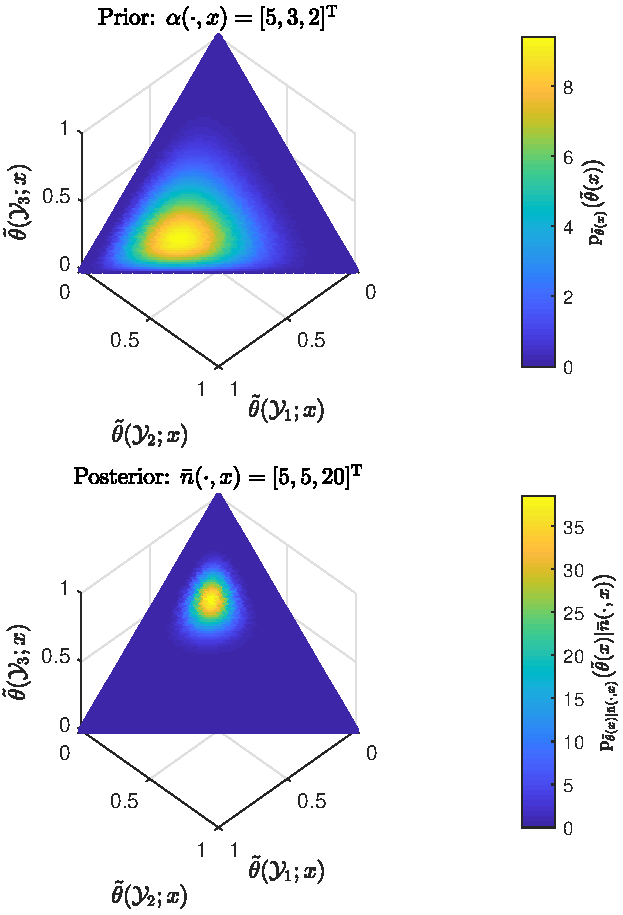
\includegraphics[width=0.7\linewidth]{P_theta_post_tilde.pdf}
\caption{Model PDF, prior and posterior}
%\label{fig:P_theta_D}
\end{figure}





\section{Model Estimation Perspective} \label{sec:predictive_est}

\todohi{generalize for Bayesian learners, move before Dirichlet!?}

PGR: use poster table??


It is instructive to treat the distribution $\Prm_{\yrm | \xrm,\uppsi}$ as an estimate of the unknown conditional PMF $\Prm_{\yrm | \xrm,\uptheta} \equiv \upthetac(\xrm)$ and investigate the effects of informative prior knowledge. For a given $\xrm$, the expected value of the estimate conditioned on the true model is
\begin{IEEEeqnarray}{L}
\Erm_{\uppsim,\uppsic | \upthetam,\upthetac}\big[ \Prm_{\yrm | \xrm,\uppsim,\uppsic} \big] 
\equiv \Erm_{\uppsim(\xrm),\uppsic(\xrm) | \upthetam(\xrm),\upthetac(\xrm)}\big[ \Prm_{\yrm | \xrm,\uppsim(\xrm),\uppsic(\xrm)} \big] \\ 
\quad = \Erm_{\uppsim(\xrm) | \upthetam(\xrm)} \big[\gammam(\xrm; \uppsim)\big] \alphac(\xrm) + \Erm_{\uppsim(\xrm) | \upthetam(\xrm)} \big[1 - \gammam(\xrm; \uppsim)\big] \upthetac(\xrm) \nonumber
\end{IEEEeqnarray}
where the properties of an Empirical distribution conditioned on its aggregation have been used. The result is a convex combination of the conditional data-independent distribution $\alphac(\xrm)$ and the true conditional distribution $\upthetac(\xrm)$. The convex coefficient, the expected value of $\gammam(\uppsim)$, is dependent on the ``marginal'' values $\alpham(\xrm)$ and $\upthetam(\xrm)$. Note that as the number of training samples $N$ and the true marginal value $\upthetam(\xrm)$ increase, the estimate tends towards the true conditional PMF; conversely, as the prior concentration $\alpha_0$ and marginal value $\alpha_m(\xrm)$ increase, the estimate tends toward the prior estimate $\alphac(\xrm)$.



To aid characterization of the estimator, define the random process $\Delta(\xrm;\uppsim,\uppsic,\upthetac) \equiv \Prm_{\yrm | \xrm,\uppsim,\uppsic} - \Prm_{\yrm | \xrm,\upthetac} \in \Rbb^{\Ycal}$. For a given $\xrm$, the bias of the conditional PMF estimate is
\begin{IEEEeqnarray}{rCl} \label{eq:predictive_bias}
\mathrm{Bias}(\xrm;\upthetam,\upthetac) & = & \Erm_{\uppsim, \uppsic | \upthetam,\upthetac}\big[ \Delta(\xrm;\uppsim,\uppsic,\upthetac) \big] \\
& = & \Erm_{\uppsim(\xrm) | \upthetam(\xrm)}\big[\gammam(\xrm; \uppsim)\big] \big( \alphac(\xrm) - \upthetac(\xrm) \big) \nonumber
\end{IEEEeqnarray}
and, noting that
\begin{IEEEeqnarray}{L}
\Prm_{\yrm | \xrm,\uppsim,\uppsic} - \Erm_{\uppsim,\uppsic | \upthetam,\upthetac}\big[ \Prm_{\yrm | \xrm,\uppsim,\uppsic} \big] \\
\quad = \big(1 - \gammam(\xrm; \uppsim)\big) \big(\uppsic(\xrm) - \upthetac(\xrm)\big) \nonumber \\
\qquad + \Big( \gammam(\xrm; \uppsim) - \Erm_{\uppsim | \upthetam}\big[ \gammam(\xrm; \uppsim) \big] \Big) \big(\alphac(\xrm) - \upthetac(\xrm)\big) \nonumber \;,
\end{IEEEeqnarray}
its covariance function is 
\begin{IEEEeqnarray}{L} \label{eq:predictive_cov}
\mathrm{Cov}(\xrm;\upthetam,\upthetac) = \Crm_{\uppsim,\uppsic | \upthetam,\upthetac} \big[\Prm_{\yrm | \xrm,\uppsim,\uppsic} \big] \\
\quad = \Erm_{\uppsim(\xrm) | \upthetam(\xrm)}\left[ \frac{\big(1 - \gammam(\xrm; \uppsim)\big)^2}{N \uppsim(\xrm)} \right] \big( \diag\big(\upthetac(\xrm)\big) - \upthetac(\xrm) \otimes \upthetac(\xrm) \big) \nonumber \\
\qquad + \Crm_{\uppsim(\xrm) | \upthetam(\xrm)}\big[ \gammam(\xrm; \uppsim) \big] \big( \alphac(\xrm) - \upthetac(\xrm) \big) \otimes \big( \alphac(\xrm) - \upthetac(\xrm) \big) \nonumber
\end{IEEEeqnarray}
where the properties of Empirical random processes have been used. Note that the bias is proportionate to the difference between the true conditional model and the data-independent estimate. The scaling factor tends to zero as the expected value of the estimate tends to the true model and to one when it tends to the prior estimate. Thus, higher data volume $N$ produces lower bias, while higher prior concentration $\alpha_0$ leads to higher bias. The variance tends to zero as $\alpha_0 \to \infty$ and as $N \to \infty$.

Combining the estimator bias and variance, the conditional second moments of $\Delta(\xrm;\uppsim,\uppsic,\upthetac)$ are
\begin{IEEEeqnarray}{rCl} \label{eq:predictive_del_sq}
\mathcal{E}(\xrm;\upthetam,\upthetac) & = & \Erm_{\uppsim,\uppsic | \upthetam,\upthetac} \Big[ \Delta(\xrm;\uppsim,\uppsic,\upthetac) \otimes \Delta(\xrm;\uppsim,\uppsic,\upthetac) \Big] \\
& = & \mathrm{Bias}(\xrm;\upthetam,\upthetac) \otimes \mathrm{Bias}(\xrm;\upthetam,\upthetac) + \mathrm{Cov}(\xrm;\upthetam,\upthetac) \nonumber \;.
\end{IEEEeqnarray}
As $N \to \infty$, this function tends to zero for values $x$ satisfying $\upthetam(x) > 0$. A more practical case is estimation with a finite volume of training data. Specification of the Dirichlet model prior can be interpreted as providing a distribution estimate $\alphac(x)$ and a confidence level $\alpha_0 \alpham(x)$. Higher confidence reduces error due to the variance of the estimator, but increases the error due to bias between the true model and its estimate; low confidence renders the estimate unbiased, but maximizes the estimator variance. 


Also of interest, the conditional expectation over $\xrm$ is
\begin{IEEEeqnarray}{L} \label{eq:predictive_E_del_sq}
\Erm_{\xrm | \upthetam}\Big[ \mathcal{E}(\xrm;\upthetam,\upthetac) \Big] \\
\quad = \Erm_{\xrm | \upthetam}\left[ \Erm_{\uppsim(\xrm) | \upthetam(\xrm)}\left[ \gammam(\xrm; \uppsim)^2 \right] \big( \alphac(\xrm) - \upthetac(\xrm) \big) \otimes \big( \alphac(\xrm) - \upthetac(\xrm) \big)  \right] \nonumber \\
\qquad + \Erm_{\xrm | \upthetam}\left[ \Erm_{\uppsim(\xrm) | \upthetam(\xrm)}\left[ \frac{N \uppsim(\xrm)}{\big( \alpha_0 \alpham(\xrm) + N \uppsim(\xrm) \big)^2} \right] \Big( \diag\big(\upthetac(y;\xrm)\big) - \upthetac(\xrm) \otimes \upthetac(\xrm) \Big) \right] \nonumber
\end{IEEEeqnarray}
\begin{IEEEeqnarray}{L} \label{eq:predictive_E_del_sq}
\Erm_{\xrm | \upthetam}\Big[ \mathcal{E}(\xrm;\upthetam,\upthetac) \Big] \\
\quad = \Erm_{\xrm | \upthetam}\left[ \Erm_{\uppsim(\xrm) | \upthetam(\xrm)}\left[ \gammam(\xrm; \uppsim)^2 \right] \big( \alphac(\xrm) - \upthetac(\xrm) \big) \otimes \big( \alphac(\xrm) - \upthetac(\xrm) \big)  \right] \nonumber \\
\qquad + \Erm_{\xrm | \upthetam}\left[ \Erm_{\uppsim(\xrm) | \upthetam(\xrm)}\left[ \frac{\big(1 - \gammam(\xrm; \uppsim)\big)^2}{N \uppsim(\xrm)} \right] \Big( \diag\big(\upthetac(y;\xrm)\big) - \upthetac(\xrm) \otimes \upthetac(\xrm) \Big) \right] \nonumber
\end{IEEEeqnarray}

Note that by the aggregation property of Empirical distributions, the empirical process $\uppsim(x)$ conditioned on the model $\upthetam(x)$ is distributed as
\begin{IEEEeqnarray}{rCl}
\Prm_{\uppsim(x) | \upthetam(x)}\big(\psim(x) | \thetam(x) \big) & = & \Emp\Big( \big(\psim(x),1-\psim(x)\big); N, \big(\thetam(x),1-\thetam(x)\big) \Big) \nonumber \\
& = & \Bi\big(N \psim(x); N, \thetam(x)\big) \;,
\end{IEEEeqnarray}
where $\Bi$ is the binomial PMF.

\todohigh{REDO FIGURES for new formulae?!}

To exemplify how the model estimate $\Prm_{\yrm | \xrm,\uppsi}$ approximates $\Prm_{\yrm | \xrm,\uptheta}$, consider a scenario with $|\Ycal| = 10$ and $|\Xcal| = 1$ for simplicity. The data-independent PMF $\alphac(x)$ and true model $\upthetac(x)$ are shown in Figure \ref{fig:P_yx_error_N_0} - note the significant mismatch. 


Figures \ref{fig:P_yx_error_a0_0_1} and \ref{fig:P_yx_error_a0_10} show how the bias and variance of the estimate change for different values of $N \uppsim(x)$ and $\alpha_0 \alpham(x)$. The plot markers represent the conditional mean of the estimator, $\Erm_{\uppsic | \uppsim,\upthetac}\big[ \Prm_{\yrm | \xrm,\uppsim,\uppsic} \big]$; the upper and lower error bars represent the square-root of the expected squared deviation above and below the conditional mean, respectively. Each individual plot heading provides the error $\sqrt{\sum_{y \in \Ycal} \mathcal{E}(y,y ; \xrm;\uppsim,\upthetac)}$ to assess the quality of the PMF estimate. 

Observe that for $N \uppsim(x) = 1$, the high variance of the $\alpha_0 \alpham(x) = 0.1$ estimate (favoring the empirical PMF) renders it worse than the $\alpha_0 \alpham(x) = 10$ estimate; in fact, the variance is so high that the error exceeds that of the data-independent estimate $\alphac(x)$ (Figure \ref{fig:P_yx_error_N_0}). Conversely, for $N \uppsim(x) = 10$, the confidence of the $ \alpha_0 \alpham(x) = 10$ estimate leads to high bias and the $ \alpha_0 \alpham(x) = 0.1$ estimate is superior. For $N \uppsim(x) = 100$, both the $ \alpha_0 \alpham(x) = 0.1$ and $ \alpha_0 \alpham(x) = 10$ estimates begin converging to the true distribution - this is guaranteed due to the full support of the Dirichlet prior.

PGR: full support discussion?


\begin{figure}
\centering
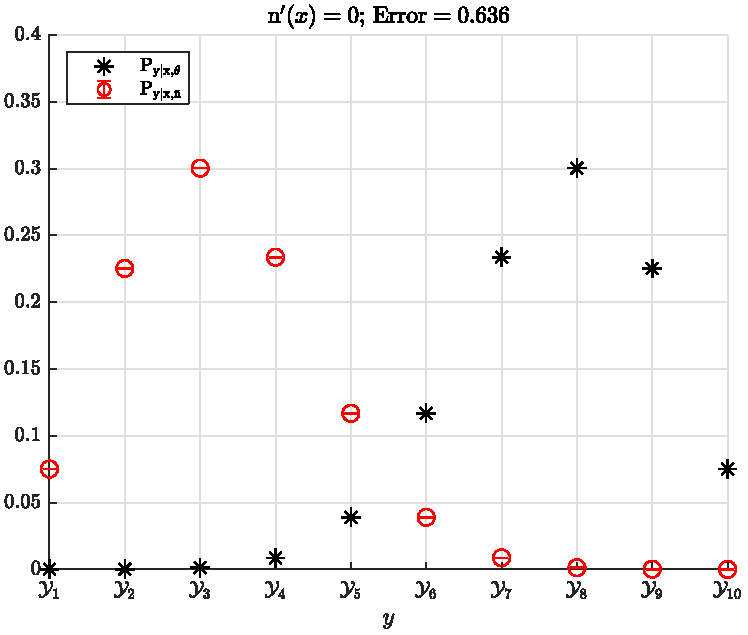
\includegraphics[width=0.7\linewidth]{P_yx_error_N_0.pdf}
\caption{Model $\uptheta$ estimate, no training data}
\label{fig:P_yx_error_N_0}
\end{figure}

\begin{figure}
\centering
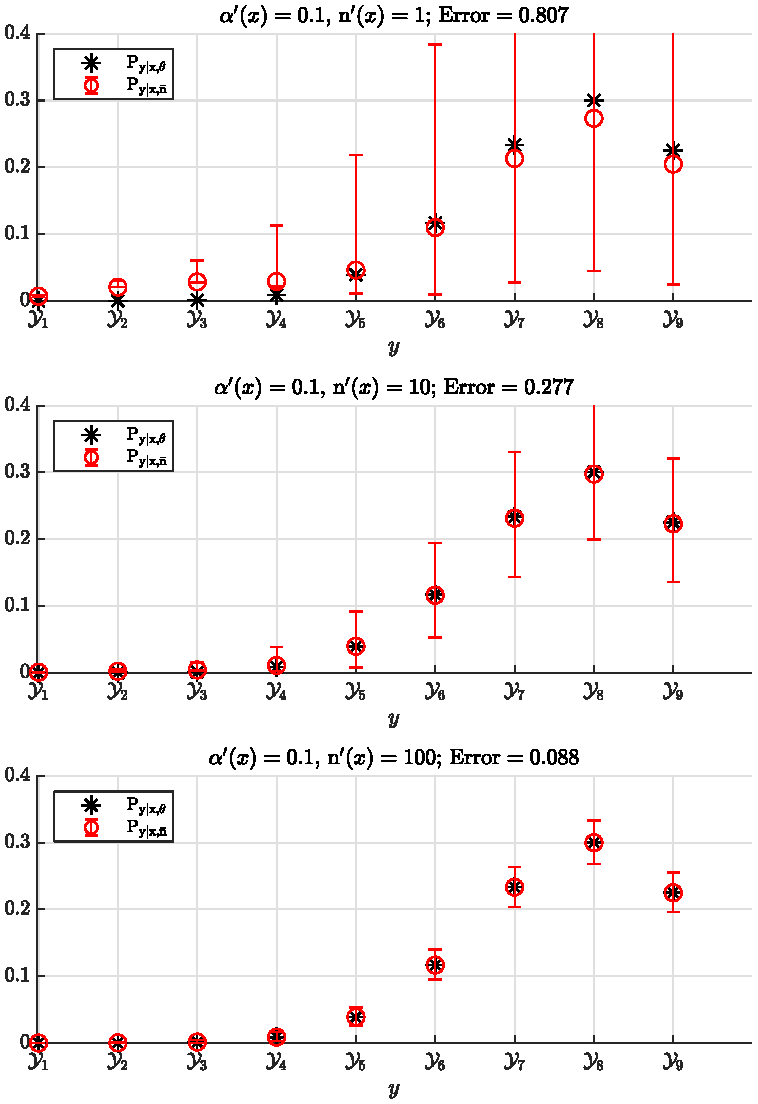
\includegraphics[width=0.7\linewidth]{P_yx_error_a0_0_1.pdf}
\caption{Model $\uptheta$ estimates, $\alpha_0 = 0.1$}
\label{fig:P_yx_error_a0_0_1}
\end{figure}

\begin{figure}
\centering
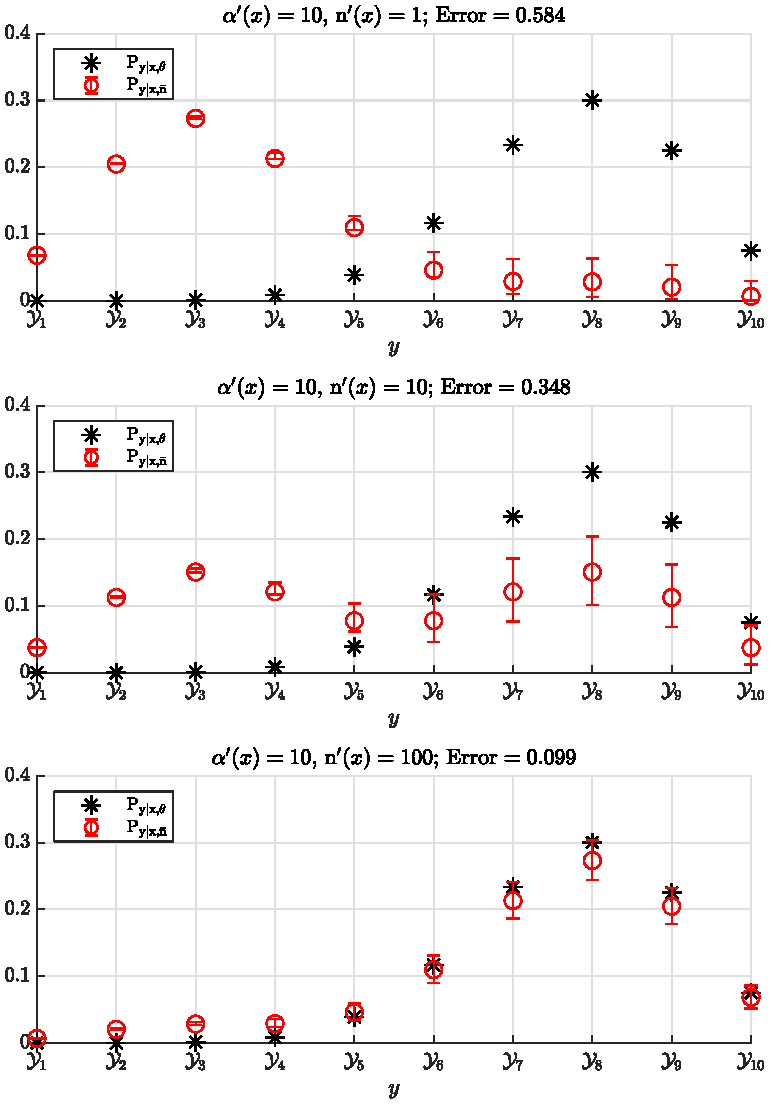
\includegraphics[width=0.7\linewidth]{P_yx_error_a0_10.pdf}
\caption{Model $\uptheta$ estimates, $\alpha_0 = 10$}
\label{fig:P_yx_error_a0_10}
\end{figure}











\newpage



\section{Applications to Common Loss Functions}

\todohigh{REPLACE bayes figs with fixed alpha0, varying learner parameterization? Should be apples-to-apples comparison!!}

\todohigh{EDIT PROGRESS!}

PGR: REMOVE GENERAL, RELOCATED MATERIAL!

PGR: equations, plots for specific theta results? informative/non-informative tradeoff??? alpha/theta mismatch results???

In this section, the Dirichlet prior is applied to the regression and classification applications. Optimal learners $f^*$ are found,  the corresponding minimum Bayes risk $\Rcal^*$ is assessed, and the conditional risk $\Rcal_{\Theta}(f^*;\theta)$ is analyzed.

PGR: add formula for f(D)??? EMPIRICAL RISK DISCUSS, REGULARIZING weight

It is useful to substitute the Bayes predictive distribution using the Dirichlet prior \eqref{eq:P_y_xD_dir} into Equation \eqref{eq:f_opt_xD}, expressing the decision for a given input $\xrm$ and training set $\Drm$ as
\begin{IEEEeqnarray}{L} \label{eq:E_y|xD L}
f^*(\xrm;\Drm) = \argmin_{h \in \Hcal} \Erm_{\yrm | \xrm,\Drm} \big[ \Lcal(h,\yrm) \big] \\
= \argmin_{h \in \Hcal} \frac{\alpha_0 \sum_{y \in \Ycal} \alpha(y,\xrm) \Lcal(h,y) + N \sum_{y \in \Ycal} \Psi(y,\xrm;\Drm) \Lcal(h,y)}{\alpha_0 \alpham(\xrm) + N \Psim(\xrm;\Drm)} \nonumber \\
= \argmin_{h \in \Hcal} \left(\frac{\alpha_0 \alpham(\xrm)}{\alpha_0 \alpham(\xrm) + N \Psim(\xrm;\Drm)}\right) \sum_{y \in \Ycal} \alphac(y;\xrm) \Lcal(h,y) + \left(\frac{N \Psim(\xrm;\Drm)}{\alpha_0 \alpham(\xrm) + N \Psim(\xrm;\Drm)}\right) \sum_{y \in \Ycal} \Psic(y;\xrm;\Drm) \Lcal(h,y) \nonumber \\
= \argmin_{h \in \Hcal} \gammam(\xrm; \uppsim) \sum_{y \in \Ycal} \alphac(y;\xrm) \Lcal(h,y) + \big(1-\gammam(\xrm; \uppsim)\big) \sum_{y \in \Ycal} \Psic(y;\xrm;\Drm) \Lcal(h,y) \nonumber \\
= \argmin_{h \in \Hcal} \gammam(\xrm; \uppsim) \Erm_{\yrm | \xrm}\big[ \Lcal(h,\yrm) \big] + \big(1-\gammam(\xrm; \uppsim)\big) \frac{\sum_{n=1}^N \delta\big[ \xrm,\Xrm_n \big] \Lcal\big( h,\Yrm_n \big)}{\sum_{n=1}^N \delta\big[ \xrm,\Xrm_n \big]} \nonumber \;.
\end{IEEEeqnarray}

The metric to be minimized can be represented as a convex combination of two expected losses. The first expected loss is evaluated with respect to the conditional distribution $\Prm_{\yrm | \xrm} = \alphac(\xrm)$, which reflects the prior knowledge of the model parameter. The second term is the conditional empirical risk, or the average loss among samples $\Yrm_n$ whose corresponding values $\Xrm_n$ match the observed value $\xrm$. The convex weights are inherited from the conditional distribution $\Prm_{\yrm | \xrm,\Drm}$; thus, for a given observation $\xrm$, the model prior concentration $\alpha_0 \alpham(\xrm)$ and the number of matching training samples $N \Psim(\xrm;\Drm)$ dictate which of the two expectations are emphasized.




\subsection{Regression: the Squared-Error Loss}

PGR: Use finite hypothesis space instead, wait for continuous DP???

PGR: add Dir conditional risk and analysis!!!

The elements of the finite cardinality set $\Ycal$ are real numbers, such that $\Ycal \subset \Rbb$. Again, $\Hcal = \Rbb \supset \Ycal$.




\subsubsection{Optimal Estimate: the Posterior Mean}

\todohi{add mean/var plots with true model, derived from model est. sec., similar to Theodoridis-ML!?}

Substituting in the Bayes predictive distribution for a Dirichlet prior \eqref{eq:P_y_xD_dir} into \eqref{eq:f_opt_SE}, the optimal Bayesian estimate is
\begin{IEEEeqnarray}{rCl} \label{eq:f_opt_SE_dir}
f^*(\xrm;\Drm) & = & \mu_{\yrm | \xrm,\Drm} \\
& = & \gammam(\xrm; \uppsim) \sum_{y \in \Ycal} y \alphac(y;\xrm) + \big(1-\gammam(\xrm; \uppsim)\big) \sum_{y \in \Ycal} y \Psic(y;\xrm;\Drm) \nonumber \\
& = & \left( \frac{\alpha_0 \alpham(\xrm)}{\alpha_0 \alpham(\xrm) + N \Psim(\xrm;\Drm)} \right) \mu_{\yrm | \xrm} + \left( \frac{N \Psim(\xrm;\Drm)}{\alpha_0 \alpham(\xrm) + N \Psim(\xrm;\Drm)} \right) \frac{\sum_{n=1}^N \delta\big[ \xrm,\Xrm_n \big] \Yrm_n}{\sum_{n=1}^N \delta\big[ \xrm,\Xrm_n \big]} \nonumber \;.
\end{IEEEeqnarray}

The optimal estimate is interpreted as a convex combination of two separate estimates - the expected value of $\yrm$ conditioned on the observed $\xrm$ and the mean of the training values $\Yrm_n$ which have a value $\Xrm_n$ matching the observed value $\xrm$. The weighting factors are the same as those of $\Prm_{\yrm | \xrm,\Drm}$; thus, stronger prior information (larger $\alpha_0 \alpham(\xrm)$) provides more weight to the estimate $\mu_{\yrm|\xrm}$ and more voluminous training data puts emphasis on the empirical conditional mean.





\paragraph{Uniform Prior}

The optimal estimator for a uniform prior is
\begin{IEEEeqnarray}{rCl}
f^*(\xrm;\Drm) & = & \left( \frac{|\Ycal|}{N \Psim(\xrm;\Drm) + |\Ycal|} \right) \frac{1}{|\Ycal|} \sum_{y \in \Ycal} y + \left( \frac{N \Psim(\xrm;\Drm)}{N \Psim(\xrm;\Drm) + |\Ycal|} \right) \sum_{y \in \Ycal} y \Psic(y;\xrm;\Drm) \\
& = & \left( \frac{|\Ycal|}{N \Psim(\xrm;\Drm) + |\Ycal|} \right) \frac{1}{|\Ycal|} \sum_{y \in \Ycal} y + \left( \frac{N \Psim(\xrm;\Drm)}{N \Psim(\xrm;\Drm) + |\Ycal|} \right) \frac{\sum_{n=1}^N \delta\big[ \xrm,\Xrm_n \big] \Yrm_n}{\sum_{n=1}^N \delta\big[ \xrm,\Xrm_n \big]} \nonumber \;.
\end{IEEEeqnarray}
Now, the model prior contribution to the weighting factors depends on the cardinality $|\Ycal|$ and the prior expectation is simply the average of the elements of $\Ycal$.




\subsubsection{Minimum Risk: the Expected Posterior Variance}

PGR: determine irreducible risk separately, before??


The minimum Bayes squared-error is $\Rcal^* = \Erm_{\xrm,\Drm} \left[ \Sigma_{\yrm | \xrm,\Drm} \right]$. Using the sufficient statistic $\uppsi \equiv \Psi(\Drm)$, the minimum risk can also be represented as $\Erm_{\xrm,\uppsi} \left[ \Sigma_{\yrm | \xrm,\uppsi} \right]$; as such, the expectations are performed over $\uppsi$. Decompose the conditional variance as
\begin{IEEEeqnarray}{rCl}
\Sigma_{\yrm | \xrm,\uppsi} & = & \Erm_{\yrm | \xrm,\uppsi}[\yrm^2] - \mu_{\yrm | \xrm,\uppsi}^2 
\end{IEEEeqnarray}
and assess the expected values of these terms separately using distributions derived from the Dirichlet prior. The first term is simply
\begin{IEEEeqnarray}{rCl}
\Erm_{\xrm,\uppsi} \left[ \Erm_{\yrm | \xrm,\uppsi}[\yrm^2] \right] & = & \Erm_{\yrm}[\yrm^2] = \sum_{y \in \Ycal} y^2 \left( \sum_{x \in \Xcal} \alpha(y,x) \right) \nonumber \\
& = & \Erm_{\xrm} \big[ \Erm_{\yrm | \xrm} [ \yrm^2 ] \big] = \sum_{x \in \Xcal} \alpham(x) \sum_{y \in \Ycal} y^2 \alphac(y;x) \nonumber \;,
\end{IEEEeqnarray}
where the different functions of $\alpha$ are represented by the PMF's of $\yrm$ and $\xrm$. Next, find, 
\begin{IEEEeqnarray}{rCl}
\Erm_{\xrm,\uppsi} \Big[ \mu_{\yrm | \xrm,\uppsi}^2 \Big] & \equiv & \Erm_{\xrm} \left[ \Erm_{\uppsic,\uppsim | \xrm} \left[ \frac{\big( \alpha_0 \alpham(\xrm) \mu_{\yrm|\xrm} + N \uppsim(\xrm) \sum_{y \in \Ycal} y \uppsic(y;\xrm) \big)^2}{\alpha_0 \alpham(\xrm) \big(\alpha_0 \alpham(\xrm) + N \uppsim(\xrm) \big)^2} \right] \right] \\
& = & \Erm_{\xrm} \left[ \Erm_{\uppsic,\uppsim} \left[ \frac{\big( \alpha_0 \alpham(\xrm) \mu_{\yrm|\xrm} + N \uppsim(\xrm) \sum_{y \in \Ycal} y \uppsic(y;\xrm) \big)^2}{\alpham(\xrm) \big(\alpha_0 \alpham(\xrm) + N \uppsim(\xrm) \big) (\alpha_0+N)} \right] \right] \nonumber \\
& = & \Erm_{\xrm} \left[ \Erm_{\uppsim} \left[ \frac{\Erm_{\uppsic | \uppsim} \left[ \big( \alpha_0 \alpham(\xrm) \mu_{\yrm|\xrm} + N \uppsim(\xrm) \sum_{y \in \Ycal} y \uppsic(y;\xrm) \big)^2 \right]}{\alpham(\xrm) \big(\alpha_0 \alpham(\xrm) + N \uppsim(\xrm) \big) (\alpha_0+N)} \right] \right] \nonumber \\
& = & \ldots \nonumber \\
& = & \Erm_{\xrm} \left[ \frac{\Erm_{\uppsim} \Big[ N \uppsim(\xrm) \Erm_{\yrm|\xrm}[\yrm^2] + \big( \alpha_0 \alpham(\xrm) + N \uppsim(\xrm) + 1 \big) \alpha_0 \alpham(\xrm) \mu_{\yrm|\xrm}^2 \Big]}{\alpham(\xrm) \big(\alpha_0 \alpham(\xrm) + 1 \big) (\alpha_0+N)} \right] \nonumber \\
& = & \Erm_{\xrm} \left[ \frac{N \Erm_{\yrm|\xrm}[\yrm^2] + \alpha_0 \big( \alpha_0 \alpham(\xrm) + N \alpham(\xrm) + 1 \big) \mu_{\yrm|\xrm}^2 }{\big( \alpha_0 \alpham(\xrm)+1 \big) (\alpha_0+N)} \right] \nonumber \;.
\end{IEEEeqnarray}

PGR: provide additional steps? Check psi work?!

%\begin{IEEEeqnarray}{L}
%\Erm_{\xrm,\uppsi} \Big[ \mu_{\yrm | \xrm,\uppsi}^2 \Big] =
%\sum_{y \in \Ycal} y \sum_{y' \in \Ycal} y' \Erm_{\xrm} \Big[ \Erm_{\uppsi | \xrm} \big[ \Prm_{\yrm | \xrm,\uppsi}(y | \xrm,\uppsi) \Prm_{\yrm | \xrm,\uppsi}(y' | \xrm,\uppsi) \big] \Big] \\
%= \sum_{y \in \Ycal} y \sum_{y' \in \Ycal} y' \Erm_{\xrm} \left[ \Erm_{\uppsi} \left[ \frac{\alpha_0 \big( \alpha(y,\xrm)+\uppsi(y,\xrm) \big) \big(\alpha(y',\xrm) + \uppsi(y',\xrm) \big)}{\alpha_0 \alpham(\xrm) \big(\alpha_0 \alpham(\xrm) + N \uppsim(\xrm) \big) (\alpha_0+N)} \right] \right] \nonumber \\
%= \sum_{y \in \Ycal} y \sum_{y' \in \Ycal} y' \Erm_{\xrm} \left[ \Erm_{\uppsim} \left[ \frac{\alpha_0 \Erm_{\uppsic | \uppsim} \left[ \big( \alpha(y,\xrm)+\uppsi(y,\xrm) \big) \big(\alpha(y',\xrm)+\uppsi(y',\xrm) \big) \right]}{\alpha_0 \alpham(\xrm) \big(\alpha_0 \alpham(\xrm) + N \uppsim(\xrm) \big) (\alpha_0+N)} \right] \right] \nonumber \\
%= \ldots \nonumber \\
%= \sum_{y \in \Ycal} y \sum_{y' \in \Ycal} y' \Erm_{\xrm} \left[ \frac{\alpha_0 \Erm_{\uppsim} \Big[ \uppsim(\xrm) \alpha(y,\xrm) \delta[y,y'] + \big( \alpha_0 \alpham(\xrm) + N \uppsim(\xrm) + 1 \big) \alpha(y,\xrm) \alpha(y',\xrm) \Big]}{\alpha_0 \alpham(\xrm)^2 \big(\alpha_0 \alpham(\xrm) + 1 \big) (\alpha_0+N)} \right] \nonumber \\
%= \sum_{y \in \Ycal} y \sum_{y' \in \Ycal} y' \Erm_{\xrm} \left[ \frac{ N \alpha_0 \alpham(\xrm) \alpha(y,\xrm) \delta[y,y'] + \big( \alpha_0 \alpha_0 \alpham(\xrm) + N \alpha_0 \alpham(\xrm) + \alpha_0 \big) \alpha(y,\xrm) \alpha(y',\xrm)}{\alpha_0 \alpham(\xrm)^2 \big(\alpha_0 \alpham(\xrm) + 1 \big) (\alpha_0+N)} \right] \nonumber \\
%= \Erm_{\xrm} \left[ \frac{N \Erm_{\yrm|\xrm}[\yrm^2] + \big( \alpha_0 \alpha_0 \alpham(\xrm) + N \alpha_0 \alpham(\xrm) + \alpha_0 \big) \mu_{\yrm|\xrm}^2 }{\big( \alpha_0 \alpham(\xrm)+1 \big) (\alpha_0+N)} \right] \nonumber \;.
%\end{IEEEeqnarray}
%\begin{IEEEeqnarray}{L}
%\Erm_{\xrm,\uppsi} \Big[ \mu_{\yrm | \xrm,\uppsi}^2 \Big] =
%\sum_{\psi \in \Uppsi} \sum_{x \in \Xcal} \Prm_{\xrm,\uppsi}(x,\psi) \left( \sum_{y \in \Ycal} y \Prm_{\yrm | \xrm,\uppsi}(y | x,\psi) \right)^2 \\
%= \sum_{x \in \Xcal} \sum_{y \in \Ycal} y \sum_{y' \in \Ycal} y' \Erm_{\uppsi} \left[ \frac{\big( \alpha(y,x)+\uppsi(y,x) \big) \big(\alpha(y',x)+\uppsi(y',x) \big)}{(\alpha_0+N) \big(\alpha'(x) + \uppsim(x) \big)} \right] \nonumber \\
%= \sum_{x \in \Xcal} \sum_{y \in \Ycal} y \sum_{y' \in \Ycal} y' \Erm_{\uppsim} \left[ \frac{\Erm_{\uppsic | \uppsim} \left[ \big( \alpha(y,x)+\uppsi(y,x) \big) \big(\alpha(y',x)+\uppsi(y',x) \big) \right]}{(\alpha_0+N) \big(\alpha'(x) + \uppsim(x) \big)} \right] \nonumber \\
%= \sum_{x \in \Xcal} \sum_{y \in \Ycal} y \sum_{y' \in \Ycal} y' \frac{\Erm_{\uppsim} \Big[ \uppsim(x) \alpha'(x) \alpha(y,x) \delta[y,y'] + \alpha'(x) \big( \alpha'(x) + \uppsim(x) + 1 \big) \alpha(y,x) \alpha(y',x) \Big]}{(\alpha_0+N) \big(\alpha'(x) + 1 \big) \alpha'(x)^2} \nonumber \\
%= \sum_{x \in \Xcal} \frac{\Erm_{\uppsim} \Big[ \uppsim(x) \Erm_{\yrm|\xrm}[\yrm^2](x) + \alpha'(x) \big( \alpha'(x) + \uppsim(x) + 1 \big) \mu_{\yrm | \xrm}^2(x) \Big]}{(\alpha_0+N) \big(\alpha'(x) + 1 \big)} \nonumber \\
%= \sum_{x \in \Xcal} \frac{N \alpha'(x) \Erm_{\yrm|\xrm}[\yrm^2](x) + \alpha'(x) \big( \alpha_0 \alpha'(x) + N \alpha'(x) + 1 \big) \mu_{\yrm | \xrm}^2(x) }{\alpha_0 (\alpha_0+N) \big(\alpha'(x) + 1 \big)} \nonumber \\
%= \Erm_{\xrm} \left[ \frac{N \Erm_{\yrm|\xrm}[\yrm^2] + \big( \alpha_0 \alpha_0 \alpham(\xrm) + N \alpha_0 \alpham(\xrm) + \alpha_0 \big) \mu_{\yrm|\xrm}^2 }{(\alpha_0+N) \big( \alpha_0 \alpham(\xrm)+1 \big)} \right] \nonumber \;.
%\end{IEEEeqnarray}
%\begin{IEEEeqnarray}{L}
%\Erm_{\xrm,\uppsi} \Big[ \mu_{\yrm | \xrm,\uppsi}^2 \Big] =
%\sum_{\psi \in \Uppsi} \sum_{x \in \Xcal} \Prm_{\xrm,\uppsi}(x,\psi) \left( \sum_{y \in \Ycal} y \Prm_{\yrm | \xrm,\uppsi}(y | x,\psi) \right)^2 \\
%= \sum_{x \in \Xcal} \sum_{y \in \Ycal} y \sum_{y' \in \Ycal} y' \Erm_{\uppsi} \left[ \frac{\big( \alpha(y,x)+\uppsi(y,x) \big) \big(\alpha(y',x)+\uppsi(y',x) \big)}{(\alpha_0+N) \big(\alpha'(x) + \uppsim(x) \big)} \right] \nonumber \\
%= \sum_{x \in \Xcal} \sum_{y \in \Ycal} y \sum_{y' \in \Ycal} y' \Erm_{\uppsim} \left[ \frac{\Erm_{\uppsic | \uppsim} \left[ \big( \alpha(y,x)+\uppsi(y,x) \big) \big(\alpha(y',x)+\uppsi(y',x) \big) \right]}{(\alpha_0+N) \big(\alpha'(x) + \uppsim(x) \big)} \right] \nonumber \\
%= \sum_{x \in \Xcal} \sum_{y \in \Ycal} y \sum_{y' \in \Ycal} y' \frac{\Erm_{\uppsim} \Big[ \uppsim(x) \frac{\alpha(y,x)}{\alpha'(x)} \delta[y,y'] + \alpha'(x) \big( \alpha'(x) + \uppsim(x) + 1 \big) \frac{\alpha(y,x)}{\alpha'(x)} \frac{\alpha(y',x)}{\alpha'(x)} \Big]}{(\alpha_0+N) \big(\alpha'(x) + 1 \big)} \nonumber \\
%= \sum_{x \in \Xcal} \sum_{y \in \Ycal} y \sum_{y' \in \Ycal} y' \left(\frac{\alpha'(x)}{\alpha_0}\right)  \frac{N \frac{\alpha(y,x)}{\alpha'(x)} \delta[y,y'] + \big( N \alpha'(x) + \alpha_0 \alpha'(x) + \alpha_0 \big) \frac{\alpha(y,x)}{\alpha'(x)} \frac{\alpha(y',x)}{\alpha'(x)}}{(\alpha_0+N) \big( \alpha'(x)+1 \big)} \nonumber \\
%= \sum_{x \in \Xcal} \left(\frac{\alpha'(x)}{\alpha_0}\right)  \frac{N \left( \sum_{y \in \Ycal} \frac{\alpha(y,x)}{\alpha'(x)} y^2 \right) + \big( N \alpha'(x) + \alpha_0 \alpha'(x) + \alpha_0 \big) \left( \sum_{y \in \Ycal} \frac{\alpha(y,x)}{\alpha'(x)} y \right)^2 }{(\alpha_0+N) \big( \alpha'(x)+1 \big)} \nonumber \;.
%\end{IEEEeqnarray}
The above formulation exploits the statistical characterization of the aggregation, $\uppsim \sim \DE(N,\alpha_0,\alpham)$; also used is the property that the Dirichlet-Empirical random process $\uppsic$ conditioned on its aggregation $\uppsim$ yields independent conditional DE functions $\uppsic(x) | \uppsim(x) \sim \DE\big( N \uppsim(x),\alpha_0 \alpham(x),\alphac(x) \big)$.

PGR: move to appendix???

Finally, combine the two formulas to represent the mininum Bayes risk,
\begin{IEEEeqnarray}{L}
\Rcal^* = \Erm_{\xrm,\uppsi} \left[ \Erm_{\yrm | \xrm,\uppsi}[\yrm^2] - \mu_{\yrm | \xrm,\uppsi}^2 \right] \\
= \Erm_{\xrm} \left[ \frac{\alpha_0 \big(\alpha_0 \alpham(\xrm) + N \alpham(\xrm) + 1 \big)}{\big( \alpha_0 \alpham(\xrm)+1 \big) (\alpha_0+N)} \Sigma_{\yrm | \xrm} \right] \nonumber \\
= \Erm_{\xrm} \left[ \frac{\alpham(\xrm) + (\alpha_0+N)^{-1}}{\alpham(\xrm) + \alpha_0^{-1}} \Sigma_{\yrm | \xrm} \right] \nonumber \;.
\end{IEEEeqnarray}
The minimum risk is the expected value of the scaled conditional variance with respect to $\Prm_{\yrm | \xrm} = \alphac(\xrm)$. The expectation is taken with respect to the prior marginal distribution $\Prm_{\xrm} = \alpham$. 

The scaling factor for each term $\Sigma_{\yrm | \xrm}$ depends on the marginal $\Prm_{\xrm}$, as well as on the prior concentration $\alpha_0$ and the number of training samples $N$. Observe that with no training data ($N = 0$), the scaling factor becomes unity and the risk is $\Rcal^* = \Erm_{\xrm} \left[ \Sigma_{\yrm | \xrm} \right]$. Conversely, as $N \to \infty$, the Bayes risk is $\Rcal^* \to \Erm_{\xrm} \left[ \frac{\alpham(\xrm)}{\alpham(\xrm) + \alpha_0^{-1}} \Sigma_{\yrm | \xrm} \right]$; note that this is equivalent to the irreducible risk $\Erm_{\uptheta}\big[\Rcal_{\Theta}^*(\uptheta)\big] = \Erm_{\xrm,\uptheta} \left[ \Sigma_{\yrm | \xrm,\uptheta} \right]$. Also, as the model concentration parameter $\alpha_0 \to 0$, the risk tends to zero (for $N > 0$); as $\alpha_0 \to \infty$, the risk tends toward $\Erm_{\xrm} \left[ \Sigma_{\yrm | \xrm} \right]$.

PGR: first/second derivatives of alpha0??

To illustrate these trends, explicitly define the sets $\Ycal = \{ i/M_{\yrm} : i = 0,\ldots,M_{\yrm}-1 \}$ and $\Xcal = \{ i/M_{\xrm} : i = 0,\ldots,M_{\xrm}-1 \}$. Assume that the conditional variance $\Sigma_{\yrm | \xrm}$ is independent of $\xrm$; in this case, the squared-error becomes the conditional variance scaled by a factor dependent on the marginal distribution $\Prm_{\xrm}$, such that $\Rcal^* = \Sigma_{\yrm | \xrm} \Erm_{\xrm} \left[ \frac{\alpham(\xrm) + (\alpha_0+N)^{-1}}{\alpham(\xrm) + \alpha_0^{-1}} \right]$.  Figures \ref{fig:Risk_SE_Dir_IO_N_leg_a0} and \ref{fig:Risk_SE_Dir_IO_a0_leg_N} display how the risk changes with $N$ and $\alpha_0$ when $\alphac(\xrm)$ and $\alpham$ are fixed.

\begin{figure}
\centering
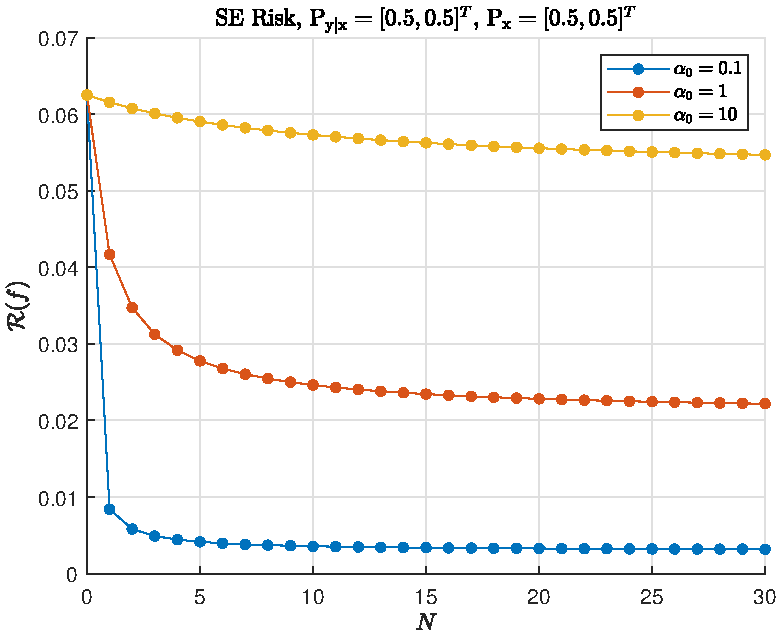
\includegraphics[width=0.7\linewidth]{Risk_SE_Dir_IO_N_leg_a0.pdf}
\caption{Minimum SE Risk for different training set sizes $N$}
\label{fig:Risk_SE_Dir_IO_N_leg_a0}
\end{figure}

\begin{figure}
\centering
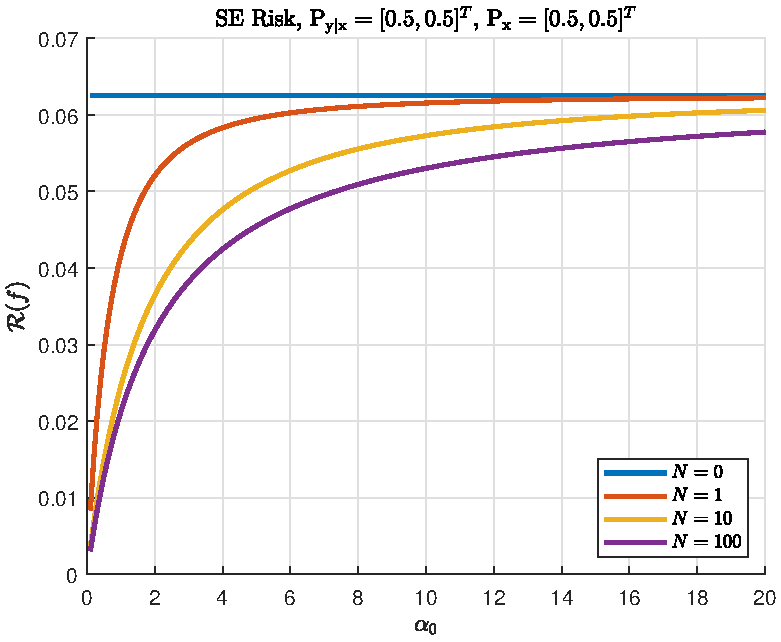
\includegraphics[width=0.7\linewidth]{Risk_SE_Dir_IO_a0_leg_N.pdf}
\caption{Minimum SE Risk for different prior concentrations $\alpha_0$}
\label{fig:Risk_SE_Dir_IO_a0_leg_N}
\end{figure}

It may not seem intutitve for the risk to decrease when $\alpha_0$ is smaller -- the variance of the model $\uptheta$ increases and the prior knowledge is less definitive. This is a result of the Dirichlet PDF weight shifting towards the $|\Ycal||\Xcal|$ models which have $\ell_0$ norms satisfying $\| \theta \|_0 = 1$. Although these PMF's are maximally separated (and uncorrelated), they all have zero variance. The optimal learner \eqref{eq:f_opt_SE_dir} will simply use the empirical distribution supplied via the training data - this allows exact identification of $\uptheta$ with a single training pair.

It is also instructional to visualize how the minimum squared-error changes for fixed volume of training data $N$ and a fixed prior concentration $\alpha_0$. First, consider how the risk changes with the conditional PMF $\alphac(\xrm)$. Figure \ref{fig:Risk_SE_Dir_IO_Pyx} demonstrates how the squared-error tends towards zero for PMFs that have $\ell_0$-norm equal to one.
\begin{figure}
\centering
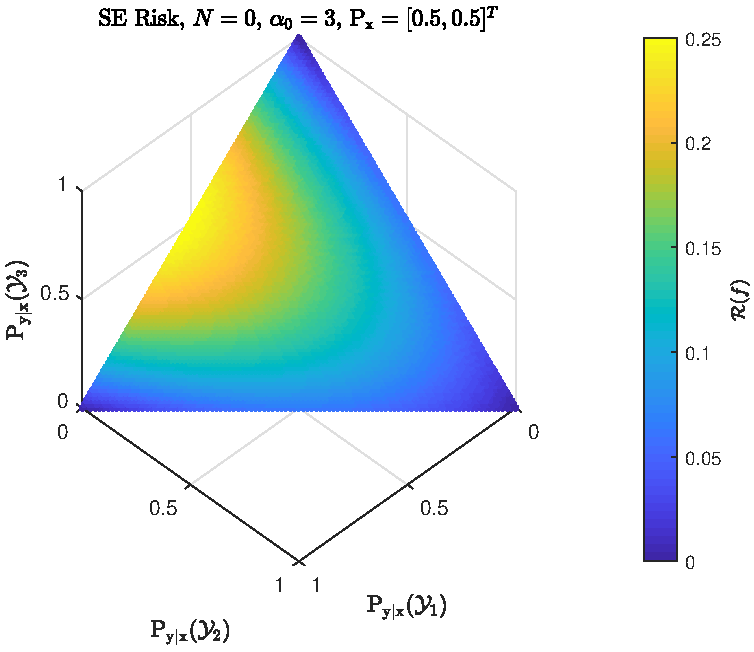
\includegraphics[width=0.7\linewidth]{Risk_SE_Dir_IO_Pyx.pdf}
\caption{Minimum SE Risk for different prior means $\Prm_{\yrm | \xrm}$}
\label{fig:Risk_SE_Dir_IO_Pyx}
\end{figure}

Next, consider the effect of the marginal distribution $\alpham$. Figure \ref{fig:Risk_SE_Dir_IO_Px_N_10_a0_1} demonstrates how the risk changes with this marginal PMF. Observe that the risk is maximal at the distributions satisfying $\| \alpham \|_0 = 1$; the scaling factor for the conditional variance $\Sigma_{\yrm | \xrm}$ becomes $\frac{1 + (\alpha_0+N)^{-1}}{1 + \alpha_0^{-1}}$. Conversely, for $\alpham = |\Xcal|^{-1}$ the scaling factor becomes $\frac{|\Xcal|^{-1} + (\alpha_0+N)^{-1}}{|\Xcal|^{-1} + \alpha_0^{-1}}$ and the risk is minimal. Figures \ref{fig:Risk_SE_Dir_IO_N_leg_Px} and \ref{fig:Risk_SE_Dir_IO_a0_leg_Px} show how different marginals $\alpham$ affect the risk as a function of $N$ and $\alpha_0$, respectively.

\begin{figure}
\centering
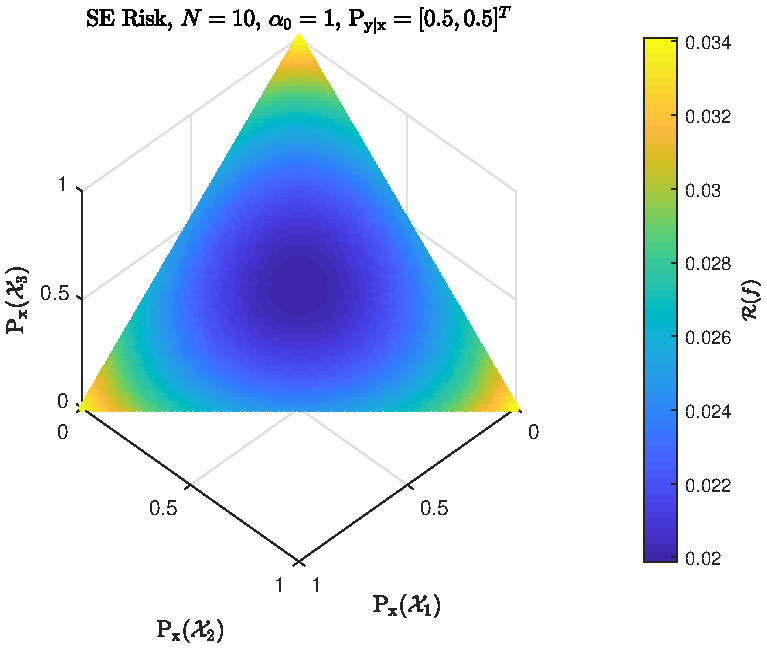
\includegraphics[width=0.7\linewidth]{Risk_SE_Dir_IO_Px_N_10_a0_1.pdf}
\caption{Minimum SE Risk for different prior means $\Prm_{\xrm}$}
\label{fig:Risk_SE_Dir_IO_Px_N_10_a0_1}
\end{figure}

\begin{figure}
\centering
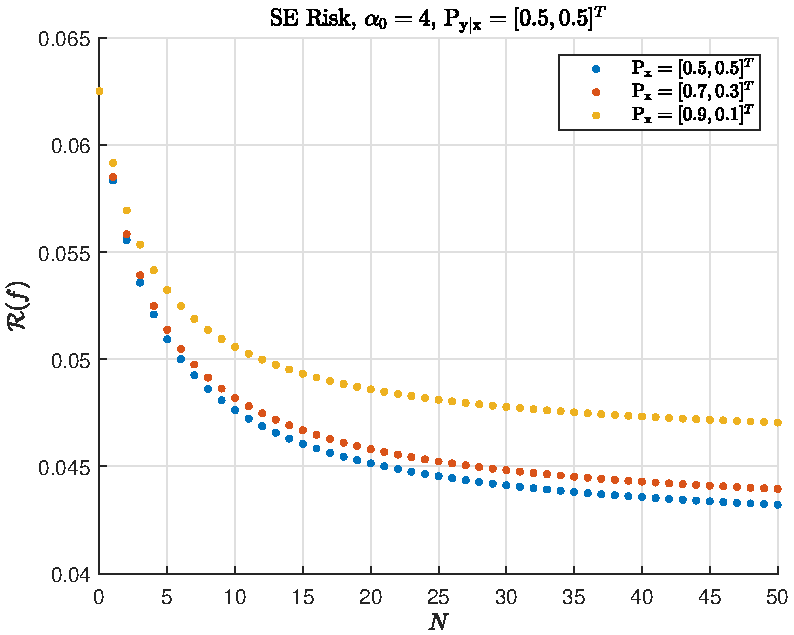
\includegraphics[width=0.7\linewidth]{Risk_SE_Dir_IO_N_leg_Px.pdf}
\caption{Minimum SE Risk for different training set volumes $N$}
\label{fig:Risk_SE_Dir_IO_N_leg_Px}
\end{figure}

\begin{figure}
\centering
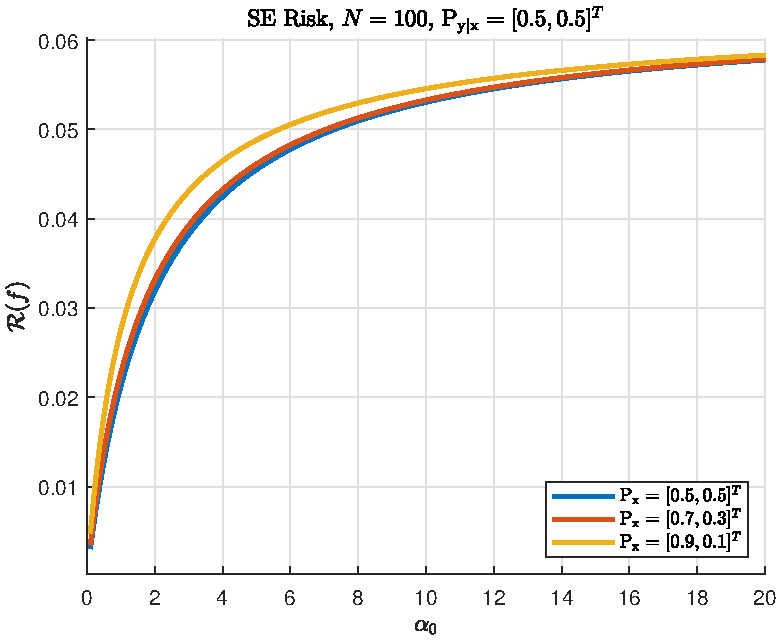
\includegraphics[width=0.7\linewidth]{Risk_SE_Dir_IO_a0_leg_Px.pdf}
\caption{Minimum SE Risk for different prior concentrations $\alpha_0$}
\label{fig:Risk_SE_Dir_IO_a0_leg_Px}
\end{figure}




\paragraph{Uniform Prior}

For the uniform model prior, the risk reduces to
\begin{IEEEeqnarray}{rCl}
\Rcal^* & = & \frac{|\Ycal| \big( N/|\Xcal| + |\Ycal| + 1 \big)}{\big( |\Ycal| + 1 \big) \big( N/|\Xcal| + |\Ycal| \big)} \left[ \left( \frac{1}{|\Ycal|} \sum_{y \in \Ycal} y^2 \right) - \left( \frac{1}{|\Ycal|} \sum_{y \in \Ycal} y \right)^2 \right] \\
& = & \frac{1 + \big( N/|\Xcal| + |\Ycal| \big)^{-1}}{1 + |\Ycal|^{-1}} \left[ \left( \frac{1}{|\Ycal|} \sum_{y \in \Ycal} y^2 \right) - \left( \frac{1}{|\Ycal|} \sum_{y \in \Ycal} y \right)^2 \right] \nonumber \;.
\end{IEEEeqnarray}
Since all possible values of $\xrm$ are equally probable and the conditional probability $\alphac(\xrm)$ is uniform and independent of $\xrm$, the risk simply becomes the variance of the set $\Ycal$ scaled by a factor dependent on $|\Ycal|$ and on $N/|\Xcal|$. Without training data ($N=0$), the scaling is unity; as $N/|\Xcal| \to \infty$, the scaling factor is $\big( 1 + |\Ycal|^{-1} \big)^{-1}$.

To visualize the performance, use the explicit sets $\Ycal$ and $\Xcal$ defined earlier. The conditional variance becomes
\begin{equation}
\Sigma_{\yrm | \xrm} = \frac{|\Ycal|^2 - 1}{12 |\Ycal|^2} = \frac{1 - |\Ycal|^{-2}}{12} 
\end{equation}
and the minimum risk is expressed as
\begin{IEEEeqnarray}{rCl}
\Rcal^* & = & \frac{\big(1 - |\Ycal|^{-1}\big) \Big(1 + \big(N/|\Xcal| + |\Ycal|\big)^{-1} \Big)}{12} \\
& = & \left(\frac{|\Ycal|}{N/|\Xcal| + |\Ycal|}\right) \frac{1 - |\Ycal|^{-2}}{12} + \left(\frac{N/|\Xcal|}{N/|\Xcal| + |\Ycal|}\right) \frac{1 - |\Ycal|^{-1}}{12} \nonumber \;.
\end{IEEEeqnarray}

Interestingly, the minimum squared-error for the uniform prior can be represented as a convex combination of two separate risk values with weighting factors dependent on $|\Ycal|$ and $N/|\Xcal|$. Thus for a uniform prior, the risk depends on the number of elements in $\Ycal$ and the number of training samples ``per element of $\Xcal$''. Note the relationship of these weighting factors to those of the conditional PMF $\Prm_{\yrm | \xrm,\Drm}$, which depend on $\alpha_0 \alpham(\xrm)$ and on $N \Psim(\xrm;\Drm)$. For the uniform prior, $\alpha_0 \alpham(\xrm) = |\Ycal|$ and $N \Erm_{\Xrm}\big[ \Psim(\Xrm) \big] = N/|\Xcal|$.

The first risk is the conditional variance $\Sigma_{\yrm|\xrm}$ - this is intuitively satisfying as the corresponding weight becomes unity when $N=0$. The second risk is the squared-error with infinite training data. Note that the reduction of the risk between these two extreme cases is modest, and that the attenuating factor increases towards unity for applications with more possible outcomes. Figure \ref{fig:Risk_SE_uniform_N_lim} illustrates the difference between these cases.

\begin{figure}
\centering
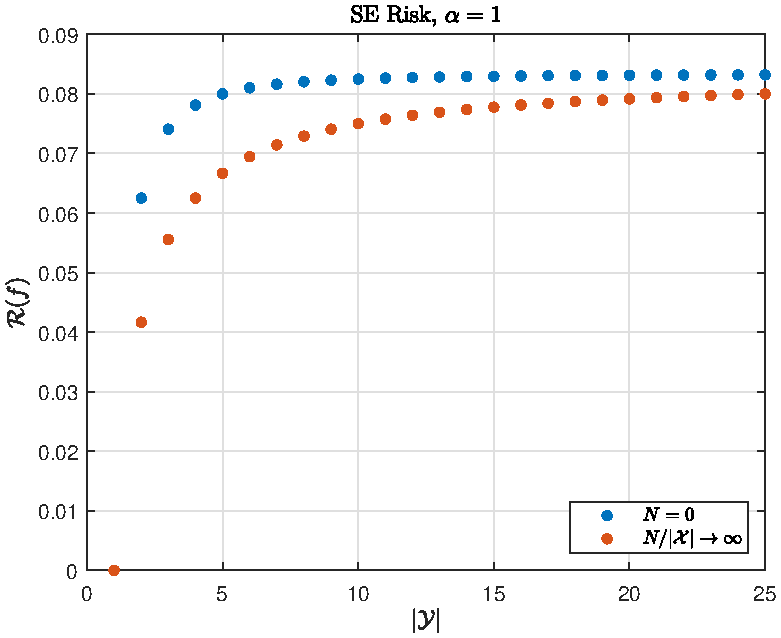
\includegraphics[width=0.7\linewidth]{Risk_SE_uniform_N_lim.pdf}
\caption{Minimum SE Risk, Uniform Prior, zero and infinite training data}
\label{fig:Risk_SE_uniform_N_lim}
\end{figure}


PGR: additional figures for uniform case?

%Figure \ref{fig:Risk_SE_IO_N} displays how the risk increases with $M_x$; Figure \ref{fig:Risk_SE_IO_N-Mx} makes the dependency on $N/M_x$ explicit.
%
%\begin{figure}
%\centering
%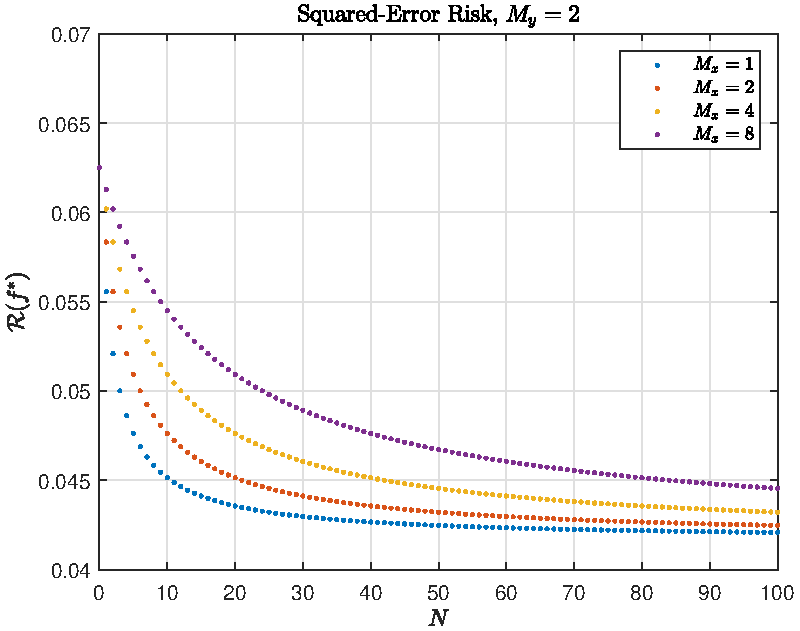
\includegraphics[width=0.7\linewidth]{Risk_SE_IO_N.pdf}
%\caption{Optimal SE Risk for different $|\Xcal|$, Uniform Prior}
%\label{fig:Risk_SE_IO_N}
%\end{figure}
%
%\begin{figure}
%\centering
%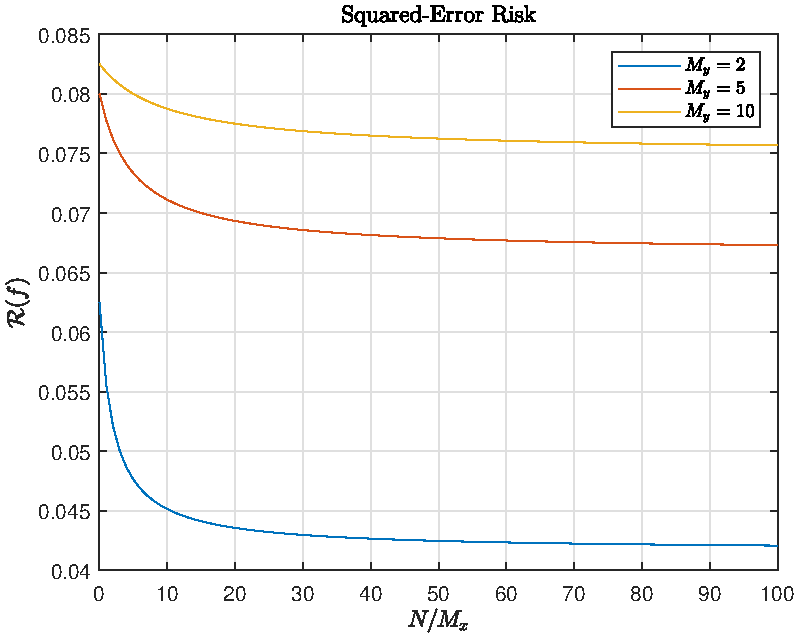
\includegraphics[width=0.7\linewidth]{Risk_SE_IO_N-Mx.pdf}
%\caption{Optimal SE Risk vs $N/|\Xcal|$, Uniform Prior}
%\label{fig:Risk_SE_IO_N-Mx}
%\end{figure}




\subsubsection{Conditional Squared-Error for a Dirichlet-based Estimator}

Having derived the optimal estimator based on a Dirichlet model prior, it is important to consider the conditional risk $\Rcal_{\Theta}(f^* ; \uptheta)$ and analyze how different prior parameterizations $\alpha$ influence the squared-error for different models $\theta$. Starting from the excess conditional squared-error risk \eqref{eq:risk_cond_ex_SE} and substituting the Bayesian estimator \eqref{eq:f_opt_SE}, the formula simplifies to $\Rcal_{\Theta, \mathrm{ex}}(f^* ; \uptheta) = \Erm_{\xrm,\Drm | \uptheta} \Big[ \big( \mu_{\yrm | \xrm,\Drm} - \mu_{\yrm | \xrm,\uptheta} \big)^2 \Big]$.

Evaluation of the excess risk for an estimator based on the Dirichlet prior will be performed using the sufficient statistic $\uppsi$ in place of the training set $\Drm$. Using the random process $\Delta(\xrm;\uppsim,\uppsic,\upthetac) \equiv \Prm_{\yrm | \xrm,\uppsim,\uppsic} - \Prm_{\yrm | \xrm,\upthetac} \in \Rbb^{\Ycal}$ introduced in \ref{sec:predictive_est}, the term is expressed as
\begin{IEEEeqnarray}{L} \label{eq:risk_cond_SE_dir_ex}
\Rcal_{\Theta, \mathrm{ex}}(f^* ; \uptheta) = \Erm_{\xrm,\Drm | \uptheta} \Big[ \big( \mu_{\yrm | \xrm,\Drm} - \mu_{\yrm | \xrm,\uptheta} \big)^2 \Big] \\
\quad \equiv \sum_{y \in \Ycal} y \sum_{y' \in \Ycal} y' \Erm_{\xrm,\uppsim,\uppsic | \upthetam,\upthetac} \Big[ \Delta(y; \xrm;\uppsim,\uppsic,\upthetac) \Delta(y'; \xrm;\uppsim,\uppsic,\upthetac) \Big] \nonumber \\
\quad = \sum_{y \in \Ycal} y \sum_{y' \in \Ycal} y' \mathcal{E}(y,y' ; \xrm,\upthetam,\upthetac) \nonumber \\
\quad = \Erm_{\xrm | \upthetam}\left[ \Sigma_{\yrm | \xrm,\upthetac} \Erm_{\uppsim(\xrm) | \upthetam(\xrm)}\left[ \frac{N \uppsim(\xrm)}{\big( \alpha_0 \alpham(\xrm) + N \uppsim(\xrm) \big)^2} \right] \right] \nonumber \\
\qquad \qquad + \Erm_{\xrm | \upthetam}\left[ \left( \mu_{\yrm | \xrm} - \mu_{\yrm | \xrm,\upthetac} \right)^2 \Erm_{\uppsim(\xrm) | \upthetam(\xrm)}\left[ \left(\frac{\alpha_0 \alpham(\xrm)}{\alpha_0 \alpham(\xrm) + N \uppsim(\xrm)}\right)^2 \right] \right] \nonumber \\
\quad = \Erm_{\xrm | \upthetam}\left[ \Sigma_{\yrm | \xrm,\upthetac} \Erm_{\uppsim(\xrm) | \upthetam(\xrm)}\left[ \frac{\big(1 - \gammam(\xrm; \uppsim\big)^2}{N \uppsim(\xrm)} \right] \right] \nonumber \\
\qquad \qquad + \Erm_{\xrm | \upthetam}\left[ \left( \mu_{\yrm | \xrm} - \mu_{\yrm | \xrm,\upthetac} \right)^2 \Erm_{\uppsim(\xrm) | \upthetam(\xrm)}\left[ \gammam(\xrm; \uppsim)^2 \right] \right] \nonumber \;,
%\quad = \Erm_{\xrm | \uptheta}\left[ \Sigma_{\yrm | \xrm,\uptheta} \Erm_{\uppsim(\xrm) | \uptheta}\left[ \frac{\alpha_0^{-2} \uppsim(\xrm)}{\big( \Prm_{\xrm}(\xrm) + \alpha_0^{-1} \uppsim(\xrm) \big)^2} \right] \right] \nonumber \\
%\qquad \qquad + \Erm_{\xrm | \uptheta}\left[ \left( \mu_{\yrm | \xrm} - \mu_{\yrm | \xrm,\uptheta} \right)^2 \Erm_{\uppsim(\xrm) | \uptheta}\left[ \left(\frac{\Prm_{\xrm}(\xrm)}{\Prm_{\xrm}(\xrm) + \alpha_0^{-1} \uppsim(\xrm)}\right)^2 \right] \right] \nonumber \;,
\end{IEEEeqnarray}
where the function $\mathcal{E}$ is defined in \eqref{eq:predictive_del_sq}. 

\todolo{note use of new model estimation formulas!}
\todomid{use weight notation from conf paper? add theta dependency to lambda}

The excess conditional risk can thus be represented as the conditional expectation (with respect to $\Prm_{\xrm | \uptheta} = \upthetam$) of a sum of two functions of $\xrm$. The first function measures the additional variance beyond that of the clairvoyant estimator (i.e. the clairvoyant squared-error); like the clairvoyant risk, it depends on $\Sigma_{\yrm | \xrm,\upthetac}$, the conditional variance of the clairvoyant estimate for a given observation of $\xrm$. The second function is dependent on the squared bias between the clairvoyant estimate $\mu_{\yrm | \xrm,\upthetac}$ and the data-independent estimate $\mu_{\yrm | \xrm}$. This term alone is influenced by the data-independent Bayes predictive distribution $\Prm_{\yrm | \xrm} = \alphac(\xrm)$.

These two second-order terms (of $y$) are scaled by factors dependent on the conditional prior localizations $\alpha_0 \alpham(x)$ and on $\upthetam(x)$ and $N$ via conditional expectations with respect to $\uppsim(x)$. By the aggregation property of Empirical distributions, $N \uppsim(x) | \upthetam(x) \sim \Bi \big(N,\upthetam(x)\big)$. Closed-forms have not been found for the function expectations of binomial random variables above.

PGR: binomial inverse moment review citations?


It is instructional to consider the trends of the squared-error risk \eqref{eq:risk_cond_SE_dir_ex} with training data volume $N$ and with Dirichlet prior parameterization.


First consider how the excess risk changes with the training volume $N$. For $N=0$, it is evident that the excess risk is $\Rcal_{\Theta, \mathrm{ex}}(f^* ; \uptheta) \to \Erm_{\xrm | \uptheta}\left[ \left( \mu_{\yrm | \xrm} - \mu_{\yrm | \xrm,\uptheta} \right)^2 \right]$,  the expected squared bias between the clairvoyant and data-independent estimators. As $N$ tends to infinity, the binomial distribution controlling the scaling factors concentrates such that $\uppsim(x) \approx \thetam(x)$; thus for $\thetam(x) > 0$, the two expectations of interest tend to zero and thus $\Rcal_{\Theta, \mathrm{ex}}(f^* ; \uptheta) \to 0$. This desirable estimator property is a consequence of the full support of the Dirichlet prior, ensuring that the model posterior concentrates at the empirical PMF.

Another interesting point regarding the dependency of the excess conditional risk on $N$ is that there may be a local maximum, depending on the learner parameterization. To demonstrate, consider the case of $|\Xcal| = 1$ - treating $N$ as a real number, there would be a maximum at 
\begin{equation}
N = \alpha_0 \left( 1 - 2 \alpha_0 \frac{\left( \mu_{\yrm | \xrm} - \mu_{\yrm | \xrm,\upthetac} \right)^2}{\Sigma_{\yrm | \xrm,\upthetac}} \right) \;.
\end{equation}
\todohi{CHECK, consider x dependency + below}
Note that as the squared-bias of the prior mean increases relative to the clairvoyant estimator variance, the maximizing value decreases (even below zero). Thus, the worse the prior estimate, the more likely the excess squared-error will decrease monotonically with $N$. Conversely, if the prior estimate is accurate, a local maximum may occur and additional training data may (temporarily) compromise the estimator performance. Also consider the effect of prior concentration; informative priors with sufficiently high $\alpha_0$ will not have the local maxima.

The excess risk at this potentially non-integral value would be 
\begin{equation}
\Rcal_{\Theta, \mathrm{ex}}(f^* ; \uptheta) \to \frac{\Sigma_{\yrm | \xrm,\uptheta}}{4 \alpha_0 \left( 1 - \alpha_0 \frac{\left( \mu_{\yrm | \xrm} - \mu_{\yrm | \xrm,\uptheta} \right)^2}{\Sigma_{\yrm | \xrm,\uptheta}} \right)} \;.
\end{equation}

PGR: better form above???

Figures \ref{fig:Risk_cond_SE_Dir_N_leg_a0_unbiased} and \ref{fig:Risk_cond_SE_Dir_N_leg_a0_biased} exemplify the excess conditional squared-error as a function of $N$ for estimators based on Dirichlet priors of varying concentration $\alpha_0$. The former shows local maxima for an unbiased estimator; note that higher concentration results in superior performance. The latter uses biased estimators and as such, learners based on low concentration achieve lower risk.
\begin{figure}
\centering
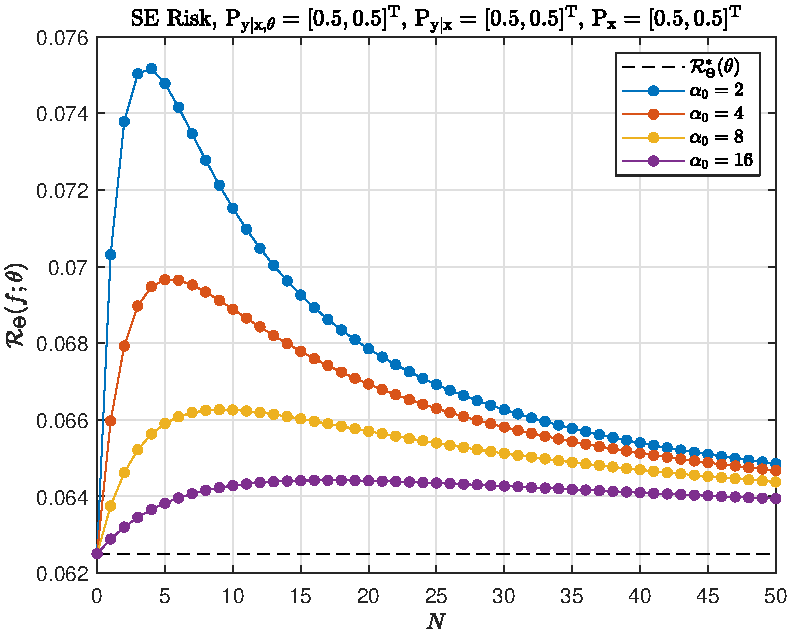
\includegraphics[width=0.7\linewidth]{Risk_cond_SE_Dir_N_leg_a0_unbiased.pdf}
\caption{Conditional SE Risk versus $N$, unbiased Dirichlet estimators of varying concentration}
\label{fig:Risk_cond_SE_Dir_N_leg_a0_unbiased}
\end{figure}
\begin{figure}
\centering
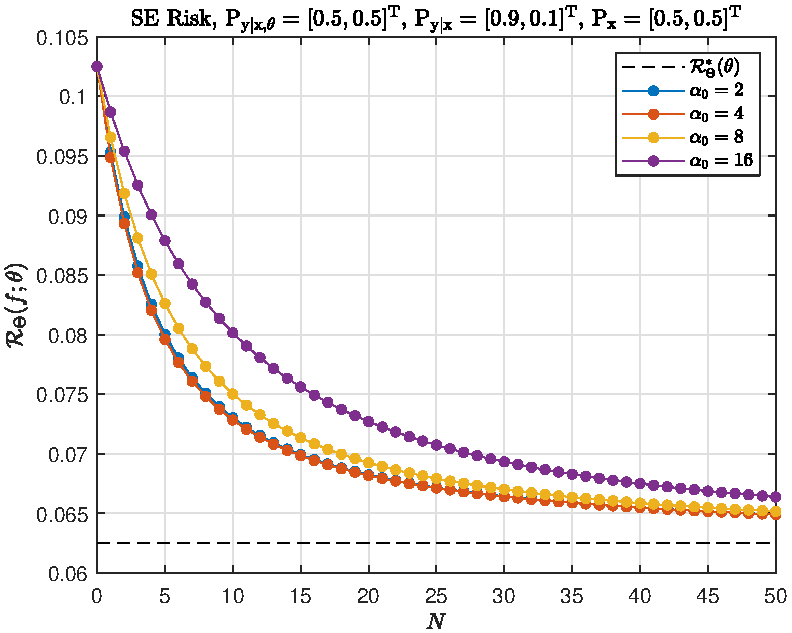
\includegraphics[width=0.7\linewidth]{Risk_cond_SE_Dir_N_leg_a0_biased.pdf}
\caption{Conditional SE Risk versus $N$, biased Dirichlet estimators of varying concentration}
\label{fig:Risk_cond_SE_Dir_N_leg_a0_biased}
\end{figure}







Next consider the effects of the Dirichlet prior parameters. The analysis will interpret the Dirichlet parameters as the conditional prior distributions $\alphac(x)$ and the corresponding concentrations $\alpha'(x) \equiv \alpha_0 \alpham(x)$. 

First consider the conditional prior PMF's $\alphac(x)$; as shown, they manifest themselves in the risk through the squared estimator bias. It is clear that regardless of how the values $\alpha_0$ and $\alpham(x)$ are chosen, the best selections for these conditional priors must have first moments matching those of the corresponding clairvoyant predictive distributions $\Prm_{\yrm | \xrm,\uptheta}$ for each $x \in \Xcal$. The resultant estimators $\mu_{\yrm | \xrm}$ are unbiased and the excess conditional risk is equivalent to the first term in \eqref{eq:risk_cond_SE_dir_ex}, measuring additional variance due to model uncertainty.



The other user-selected Dirichlet parameters manifest themselves in the conditional risk as $\alpha'(x)$, the concentrations of the corresponding conditional distributions $\upthetac(x)$; these values control important bias/variance trade-offs via the two scaling factors in \eqref{eq:risk_cond_SE_dir_ex}. First, consider the asymptotic trends.

Consider how the excess risk tends as the priors become maximally concentrated. As $\alpha'(x) \to \infty$, the excess risk tends to $\Rcal_{\Theta, \mathrm{ex}}(f^* ; \uptheta) \to \Erm_{\xrm | \uptheta}\left[ \left( \mu_{\yrm | \xrm} - \mu_{\yrm | \xrm,\uptheta} \right)^2 \right]$, the expected conditional squared-error between the means of the Bayesian predictive PMF and the clairvoyant predictive PMF. This is intuitive given that the estimator tends toward a data-independent solution; analogous to the discussion in Section \ref{sec:predictive_est}, the estimator may be biased, but will have no variance due to the training data statistics.

Conversely, if concentrations $\alpha'(x) \to 0$ are chosen, the Bayesian estimate tends to the empirical mean, independent of $\alphac(\xrm)$, and the excess risk tends to
\begin{IEEEeqnarray}{rCl}
\Rcal_{\Theta, \mathrm{ex}}(f^* ; \uptheta) & \to & \Erm_{\xrm | \upthetam}\left[ \Sigma_{\yrm | \xrm,\upthetac} \sum_{n=1}^N \binom{N}{n} \upthetam(\xrm)^n \big( 1 - \upthetam(\xrm) \big)^{N-n} \frac{1}{n} \right] \nonumber \\
&& \qquad + \Erm_{\xrm | \upthetam}\left[ \big( 1 - \upthetam(\xrm) \big)^N \left( \mu_{\yrm | \xrm} - \mu_{\yrm | \xrm,\upthetac} \right)^2 \right] \nonumber \;.
\end{IEEEeqnarray}
Note that the first term's scaling factor is equivalent to the first inverse moment of a positive binomial random variable \cite{stephan}. The second term's scaling factor tends to $\Prm_{\uppsim(\xrm) | \upthetam(\xrm)}\big( 0 | \thetam(x) \big)$, the probability that no training samples are observed matching the value $\xrm$. As $N$ increases, this term tends to zero, the risk due to the prior estimate bias decreases, and the excess risk becomes a function of $\uptheta$ only.



Of further interest are the values $\alpha'(x)$ that minimize the excess squared-error for given prior conditional distributions $\alphac(x)$. With the asymptotic values of the excess risk known, all that remains is to determine any local minima. Since the $|\Xcal|$ summands of the excess risk depend only on the corresponding concentrations $\alpha'(x)$, each of these values can be optimized separately. 

\todomid{add the derivative details below???}

Calculating the first derivative with respect to $\alpha'(x)$, it can be shown that for $N > 0$ and $\thetam(x) > 0$, only one stationary point exists, at 
\begin{equation} \label{eq:alpha_x_min_Rex}
\alpha'(\xrm) = \frac{\Sigma_{\yrm | \xrm,\upthetac}}{\left( \mu_{\yrm | \xrm} - \mu_{\yrm | \xrm,\upthetac} \right)^2} \;.
\end{equation}
Calculation of the second derivative confirms that this value is a local minimum. Furthermore, the excess risk evaluated at these values is 
\begin{equation}
\Rcal_{\Theta, \mathrm{ex}}(f^* ; \uptheta) = \Erm_{\xrm | \upthetam}\left[ \Erm_{\uppsim(\xrm) | \upthetam(\xrm)}\left[ \frac{1}{N \uppsim(\xrm) \Sigma_{\yrm | \xrm,\upthetac}^{-1} + \left( \mu_{\yrm | \xrm} - \mu_{\yrm | \xrm,\upthetac} \right)^{-2}} \right] \right] \;,
\end{equation}
which can be easily shown to be less than both the asymptotic values for $\alpha'(x) \to 0$ and $\alpha'(x) \to \infty$. Thus the concentration values \eqref{eq:alpha_x_min_Rex} can be used to find the optimal values of $\alpha_0$ and $\alpham(x)$ leading to the minimum excess risk for the given prior conditional distributions $\alphac(x)$.

Note that the minimizing concentration values $\alpha'(x)$ are inversely proportional to the squared-bias of the prior conditional mean. This is sensible; the better the match between the true and prior predictive distributions, the more confidence should be expressed. Also, low concentrations are preferable when the conditional model has low variance; these models can be accurately identified by learners that prioritize the empirical mean over the prior estimate, even with limited training data $N$. Additionally, note that these values $\alpha'(x)$ do not depend on the training volume $N$.



%\Erm_{\xrm | \uptheta}\left[ \Sigma_{\yrm | \xrm,\uptheta} \Erm_{\uppsim(\xrm) | \upthetam(\xrm)}\left[ \frac{\uppsim(\xrm)}{\big( \alpha_0 \alpham(\xrm) + N \uppsim(\xrm) \big)^2} \right] \right] \nonumber \\
%\qquad \qquad + \Erm_{\xrm | \uptheta}\left[ \left( \mu_{\yrm | \xrm} - \mu_{\yrm | \xrm,\uptheta} \right)^2 \Erm_{\uppsim(\xrm) | \upthetam(\xrm)}\left[ \left(\frac{\alpha_0 \alpham(\xrm)}{\alpha_0 \alpham(\xrm) + N \uppsim(\xrm)}\right)^2 \right] \right] \nonumber


Figures \ref{fig:Risk_cond_SE_Dir_a0_leg_N_unbiased} and \ref{fig:Risk_cond_SE_Dir_a0_leg_N_biased} show how the excess conditional squared-error trends as a function of the Dirichlet learner concentration. Note that the latter is based on a biased prior estimate and thus the optimal Dirichlet concentration value is lower.
\begin{figure}
\centering
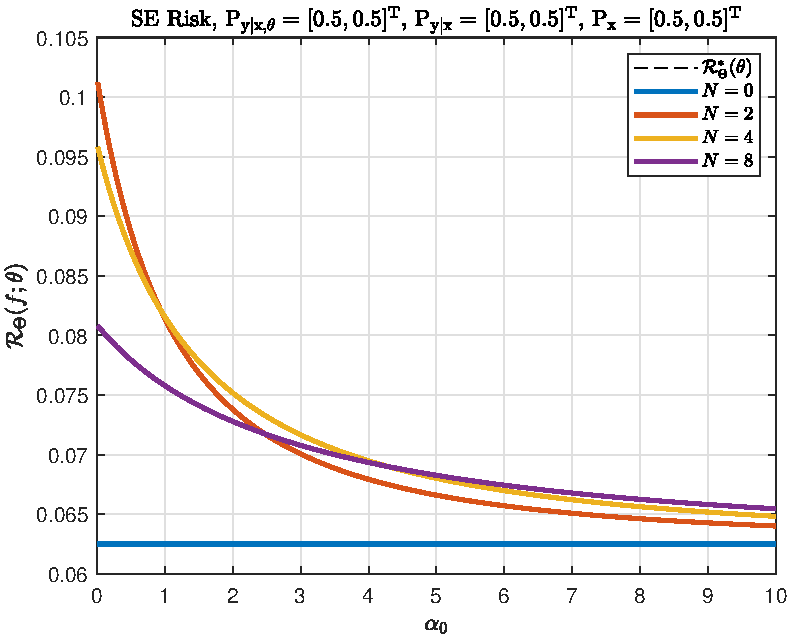
\includegraphics[width=0.7\linewidth]{Risk_cond_SE_Dir_a0_leg_N_unbiased.pdf}
\caption{Conditional SE Risk versus $\alpha_0 \alpham(x)$, unbiased Dirichlet estimator using varying training set volumes}
\label{fig:Risk_cond_SE_Dir_a0_leg_N_unbiased}
\end{figure}
\begin{figure}
\centering
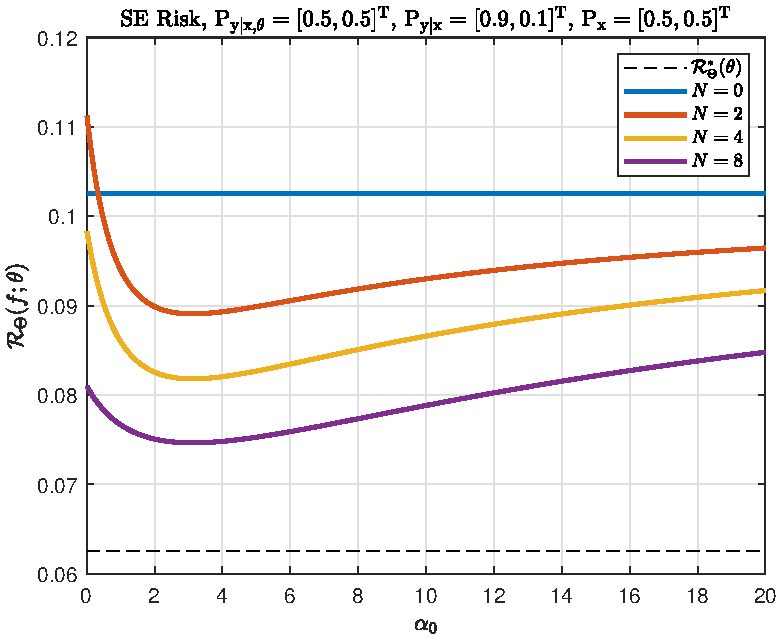
\includegraphics[width=0.7\linewidth]{Risk_cond_SE_Dir_a0_leg_N_biased.pdf}
\caption{Conditional SE Risk versus $\alpha_0$, biased Dirichlet estimator using varying training set volumes}
\label{fig:Risk_cond_SE_Dir_a0_leg_N_biased}
\end{figure}

PGR: plot captions, alpha zero or x???









\newpage

PGR: newpage






\subsection{Classification: the 0-1 Loss}

This section derives 0-1 loss classifiers based on the Dirichlet prior distribution and assesses their performance.

\subsubsection{Optimal Hypothesis: Conditional Maximum \emph{a posteriori}}

PGR: decision region figures??

PGR: weighted conditional majority decision

To determine the optimal learning function, the 0-1 loss from Equation \eqref{eq:loss_01} is substituted into Equation \eqref{eq:E_y|xD L} and Equation \eqref{eq:f_opt_xD} to find
\begin{IEEEeqnarray}{rCl} \label{eq:f_opt_01_dir}
f^*(x;D) & = & \argmax_{y \in \Ycal} \Prm_{\yrm | \xrm,\Drm}(y | x,D) \\
& = & \argmax_{y \in \Ycal} \frac{\alpha_0 \alpham(x) \alphac(y;x) + N \Psim(x;D) \Psic(y;x;D)}{\alpha_0 \alpham(x) + N \Psim(x;D)} \nonumber \\
& = & \argmax_{y \in \Ycal} \big( \alpha_0 \alpha(y,x) + N \Psi(y,x;D) \big) \nonumber \\
& = & \argmax_{y \in \Ycal} \big( \alpha_0 \alpham(x) \alphac(y;x) + N \Psim(x;D) \Psic(y;x;D) \big) \nonumber \;.
\end{IEEEeqnarray}
Using the Dirichlet prior, different classes are ``scored'' by counting the number of training samples with a value of $\Xrm_n$ matching that of $\xrm$ and combining with the prior parameters $\alpha_0$ and $\alpha(\cdot,\xrm)$.  



\paragraph{Uniform Prior}

When the uniform prior is used, the Bayes classifier simplifies to 
\begin{IEEEeqnarray}{rCl}
f^*(x;D) & = & \argmax_{y \in \Ycal} \Psic(y;x;D) \;,
\end{IEEEeqnarray}
the maximizing argument of the conditional empirical model. This effects a conditional majority decision which chooses the class from $\Ycal$ most often represented among training set samples $\Drm$ with a matching input value $\xrm$. This is intuitive, as the model PDF parameter $\alpha$ imparts no confidence as to which classes may be most likely.







\subsubsection{Minimum Risk: Probability of Error}

\todohigh{no closed-forms found??? Find closed-form BOUNDS???}


Evaluating the minimum risk \eqref{eq:risk_min_01} using the distributions derived from the Dirichlet prior, the Bayes minimum probability of error is 
\begin{IEEEeqnarray}{rCl}
\Rcal^* & = & 1 - \Erm_{\xrm,\Drm} \left[ \max_{y \in \Ycal} \Prm_{\yrm | \xrm,\Drm}(y | \xrm,\Drm) \right] \\
& = & 1 - \Erm_{\xrm,\uppsim,\uppsic} \left[ \frac{ \max_{y \in \Ycal} \big( \alpha_0 \alpham(x) \alphac(y;x) + N \uppsim(x) \uppsi(y;x) \big)}{\alpha_0 \alpham(x) + N \uppsim(x)} \right] \nonumber \\
& = & 1 - \sum_{x \in \Xcal} \frac{\Erm_{\uppsi} \Big[ \max_{y \in \Ycal} \big( \alpha_0 \alpha(y,x) + N \uppsi(y,x) \big) \Big]}{\alpha_0 + N} \nonumber \;.
\end{IEEEeqnarray}
Figures \ref{fig:Risk_01_Dir_N_leg_a0} and \ref{fig:Risk_01_Dir_a0_leg_N} plot the minimum Bayes probability of error against training data volume $N$ and prior concentration $\alpha_0$, respectively. Note that for $N = 0$, the Bayes risk is $\Rcal^* = 1 - \sum_{x \in \Xcal} \max_{y \in \Ycal} \alpha(y,x)$. Additionally, consider the risk for maximal/minimal values of the Dirichlet concentration. For $\alpha_0 \to 0$ (and $N > 1$), the risk is $\Rcal^* = 0$; conversely, for $\alpha_0 \to \infty$, the risk tends to $\Rcal^* \to 1 - \sum_{x \in \Xcal} \max_{y \in \Ycal} \alpha(y,x)$. These trends can be visualized in Figures \ref{fig:Risk_01_Dir_Pyx__a0_high} and \ref{fig:Risk_01_Dir_Pyx__a0_low}.

PGR: risk for $N \to \infty$?

PGR: missing info for Dir gen graphics? fixed y given x conditional alpha???

PGR: comment on simulation!



\begin{figure}
\centering
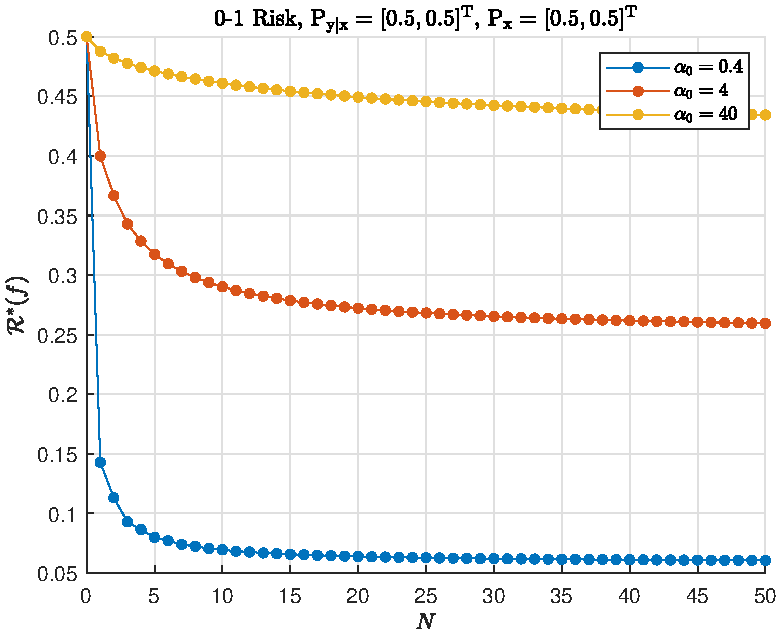
\includegraphics[width=0.7\linewidth]{Risk_01_Dir_N_leg_a0.pdf}
\caption{Minimum 0-1 Risk for different training data volumes $N$}
\label{fig:Risk_01_Dir_N_leg_a0}
\end{figure}

\begin{figure}
\centering
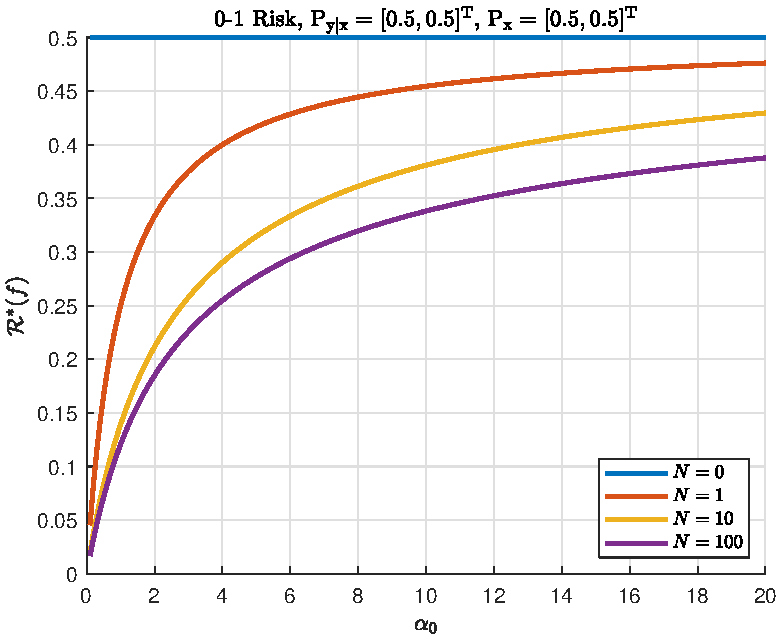
\includegraphics[width=0.7\linewidth]{Risk_01_Dir_a0_leg_N.pdf}
\caption{Minimum 0-1 Risk for different prior concentrations $\alpha_0$}
\label{fig:Risk_01_Dir_a0_leg_N}
\end{figure}

\begin{figure}
\centering
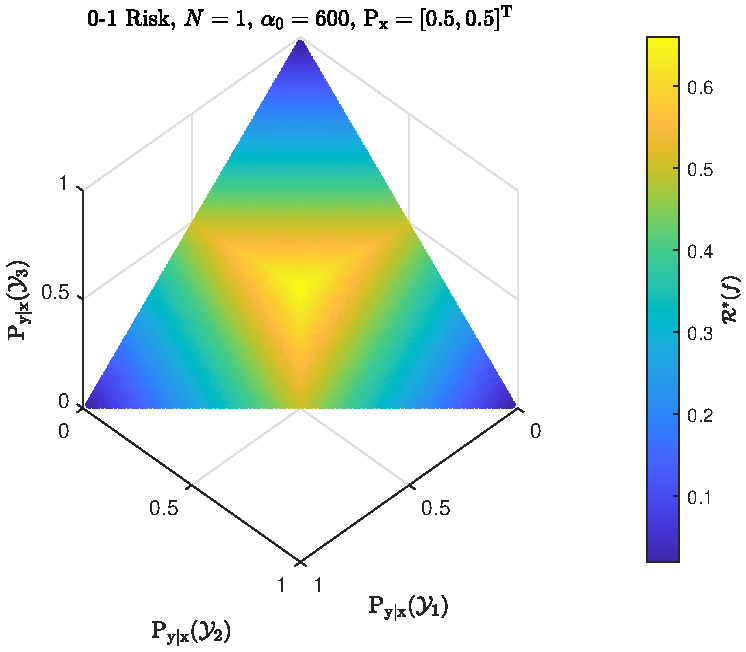
\includegraphics[width=0.7\linewidth]{Risk_01_Dir_Pyx__a0_high.pdf}
\caption{Minimum 0-1 Risk for different prior means $\Prm_{\yrm | \xrm}$}
\label{fig:Risk_01_Dir_Pyx__a0_high}
\end{figure}

\begin{figure}
\centering
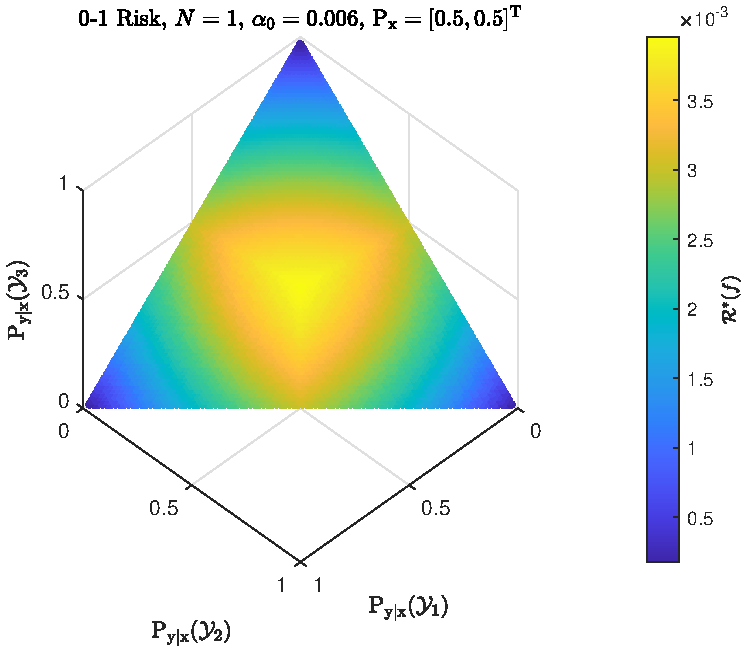
\includegraphics[width=0.7\linewidth]{Risk_01_Dir_Pyx__a0_low.pdf}
\caption{Minimum 0-1 Risk for different prior means $\Prm_{\yrm | \xrm}$}
\label{fig:Risk_01_Dir_Pyx__a0_low}
\end{figure}

%\begin{figure}
%\centering
%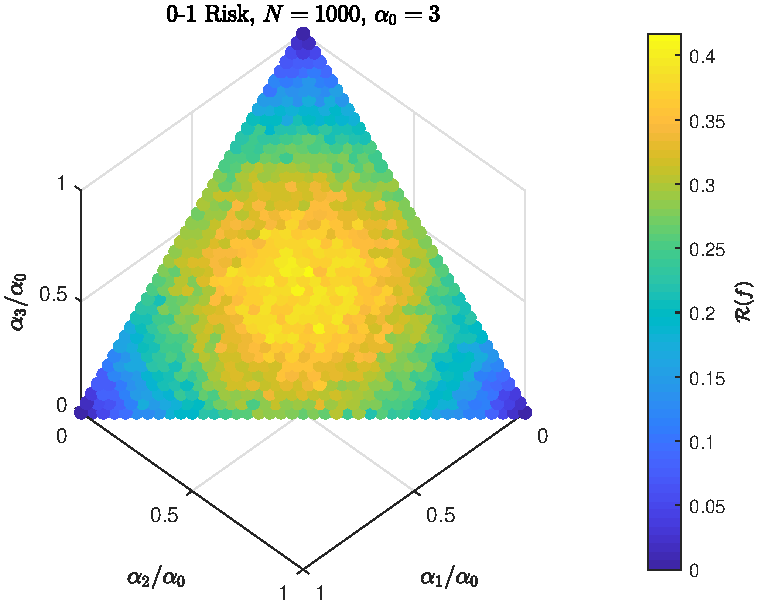
\includegraphics[width=0.7\linewidth]{Risk_01_Dir_muTheta_N_1000_a0_3.pdf}
%\caption{Minimum 0-1 Risk vs $\mu_{\uptheta}$ (sim)}
%\label{fig:Risk_01_Dir_muTheta_N_1000_a0_3}
%\end{figure}
%
%
%\begin{figure}
%\centering
%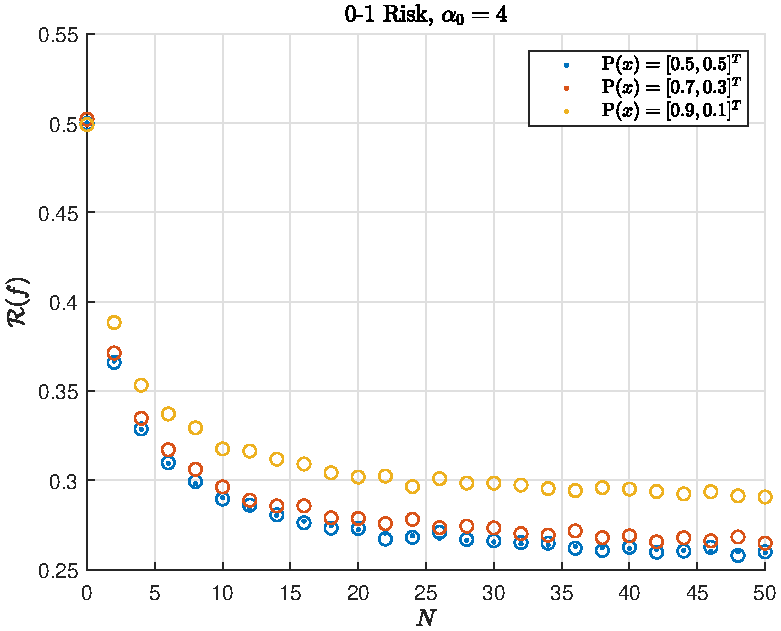
\includegraphics[width=0.7\linewidth]{Risk_01_Dir_IO_N_leg_Px.pdf}
%\caption{Minimum 0-1 Risk vs $N$ (sim)}
%\label{fig:Risk_01_Dir_IO_N_leg_Px}
%\end{figure}
%
%\begin{figure}
%\centering
%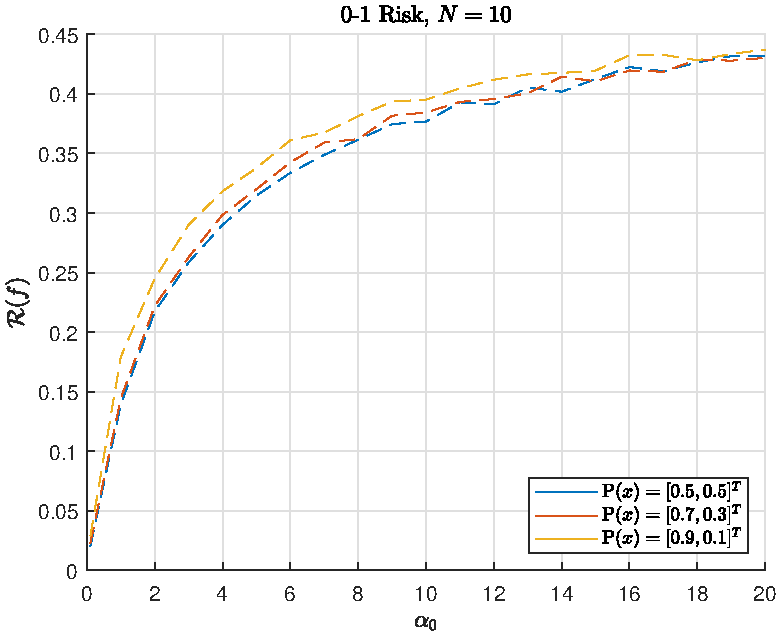
\includegraphics[width=0.7\linewidth]{Risk_01_Dir_IO_a0_leg_Px.pdf}
%\caption{Minimum 0-1 Risk vs $\alpha_0$ (sim)}
%\label{fig:Risk_01_Dir_IO_a0_leg_Px}
%\end{figure}
%
%\begin{figure}
%\centering
%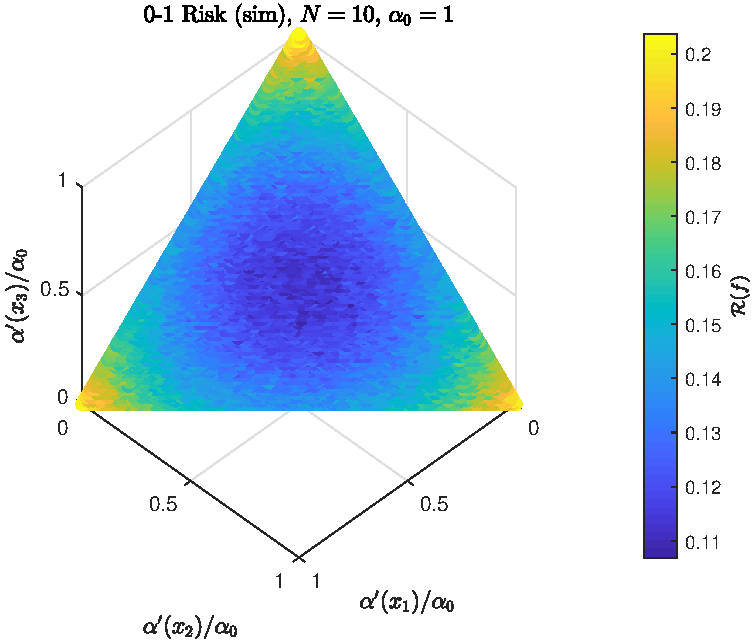
\includegraphics[width=0.7\linewidth]{Risk_01_Dir_IO_Px_N_10_a0_1.pdf}
%\caption{Minimum 0-1 Risk vs $\Prm_{\xrm}$ (sim)}
%\label{fig:Risk_01_Dir_IO_Px_N_10_a0_1}
%\end{figure}








\paragraph{Uniform Prior}

PGR: COMPUTATIONAL COMPLEXITY savings for risk formula?

PGR: Can uniform minimal risk be approximated as a function of My and Mx/N, as is for SE loss???

PGR: use Mcal not binom!

PGR: add nmax CDF fig!


Using the uniform prior, the minimum Bayes 0-1 risk is 
\begin{IEEEeqnarray}{rCl}
\Rcal^* & = & 1 - \Erm_{\xrm,\Drm} \left[ \max_{y \in \Ycal} \Prm_{\yrm | \xrm,\Drm}(y | \xrm,\Drm) \right] \\
& = & 1 - \sum_{x \in \Xcal} \frac{1 + N \Erm_{\uppsi} \big[ \max_{y \in \Ycal} \uppsi(y,x) \big]}{|\Ycal||\Xcal| + N} \nonumber \\
& = & 1 - \frac{1 + N |\Xcal|^{-1} \sum_{x \in \Xcal} \Erm_{\uppsi} \big[ \max_{y \in \Ycal} \uppsi(y,x) \big]}{|\Ycal| + N |\Xcal|^{-1}} \nonumber \\
& = & 1 - \frac{1 + N |\Xcal|^{-1} \sum_{x \in \Xcal} \Erm_{\uppsim(x)} \Big[ \uppsim(x) \Erm_{\uppsic(x) | \uppsim(x)} \big[ \max_{y \in \Ycal} \uppsic(y;x) \big] \Big]}{|\Ycal| + N |\Xcal|^{-1}} \nonumber \;.
\end{IEEEeqnarray}
The expectation operates on the maximum value from a subset of a uniform Dirichlet-Empirical random process. Via the Dirichlet-Empirical aggregation property (related to the Dirichlet-Multinomial property \cite{johnson}), a consequence of the the uniform PMF $\Prm_{\uppsi}$ is that the individual segments $\uppsi(\cdot,x)$ are identically distributed; thus, the expectation will be same for every value $x$.

To evaluate this expectation, new random variables $\uppsi_{\max}(x) \equiv \max_{y \in \Ycal} \uppsi(y,x) \in \{ n/N: n \in 0,\ldots,N \}$ are introduced and characterized by their identical PMF. To this end, the probability of the event $\Prm\big( \uppsi_{\max}(x) \geq n/N \big) = \Prm\big( \cup_{y \in \Ycal} \{ \uppsi(y,x) \geq n/N \} \big)$ will be determined. As the distribution of $\uppsi$ is uniform, the event probability is proportionate to the cardinality of the set $\cup_{y \in \Ycal} \{ \psi: \psi(y,x) \geq n/N \}$. Using the inclusion-exclusion principle \cite{brualdi}, the cardinality is represented as
\begin{IEEEeqnarray}{L}
\big| \cup_{y \in \Ycal} \{ \psi : \psi(y,x) \geq n/N \} \big| \\
\quad = \begin{cases} \binom{N+|\Ycal||\Xcal|-1}{|\Ycal||\Xcal|-1} & \mathrm{if} \ n < 0, \\ \sum_{m=1}^{|\Ycal|} \binom{|\Ycal|}{m} (-1)^{m-1} \binom{N-mn+|\Ycal||\Xcal|-1}{|\Ycal||\Xcal|-1} H\Big( \big\lfloor\frac{N}{m}\big\rfloor - n \Big) & \mathrm{if} \ 0 \leq n \leq N, \\ 0 & \mathrm{if} \ n > N, \end{cases} \nonumber
\end{IEEEeqnarray}
where $H: \Zbb \mapsto \{0,1\}$ is the discrete Heaviside step function. For $n < 0$, the cardinality is equivalent to $|\Uppsi|$. 

For $0 \leq n < N$, the cardinality is an alternating binomial summation where the $m^\mathrm{th}$ term accounts for the different intersections of $m$ of the $|\Ycal|$ individual sets $\{ \psi : \psi(y,x) \geq n/N \}$. Observe that the cardinality of the intersections is only dependent on the number of contributing sets $m$ and not on which sets intersect. Furthermore, note the dependency of the intersection cardinalities on the argument $n$. The step function contributes such that if $n > \big\lfloor\frac{N}{m}\big\rfloor$, only up to $m-1$ individual sets will intersect. The binomial coefficient $\Mcal\big( (N-mn,|\Ycal||\Xcal|-1) \big)$ provides the intersection cardinality for a given $m$; note the similarity to the cardinality $|\Uppsi|$ - the only difference is the number of points that grid the $|\Ycal||\Xcal|-1$ dimensional region.

The probability of interest can thus be expressed as
\begin{IEEEeqnarray}{L}
\Prm\big( \uppsi_{\max}(x) \geq n/N \big) = \binom{N+|\Ycal||\Xcal|-1}{|\Ycal||\Xcal|-1}^{-1} \big| \cup_{y \in \Ycal} \{ \psi : \psi(y,x) \geq n/N \} \big| \\
\quad = \begin{cases} 1 & \mathrm{if} \ n < 0, \\ \sum_{m=1}^{|\Ycal|} \binom{|\Ycal|}{m} (-1)^{m-1} \prod_{l=1}^{|\Ycal||\Xcal|-1} \Big( 1-\frac{mn}{N+l} \Big) H\Big( \big\lfloor\frac{N}{m}\big\rfloor - n \Big) & \mathrm{if} \ 0 \leq n \leq N, \\ 0 & \mathrm{if} \ n > N. \end{cases} \nonumber
\end{IEEEeqnarray}


PGR: use Mcal op?

PGR: Heaviside reference?

As the PMF of $\uppsi_{\max}(x)$ has support on $\{ n/N: n \in 0,\ldots,N \}$, the expectation over $\uppsi$ is evaluated as
\begin{IEEEeqnarray}{rCl}
\Erm_{\uppsi}\big[ \uppsi_{\max}(x) \big] & = & \sum_{n=0}^N \frac{n}{N} \Big( \Prm\big( \uppsi_{\max}(x) \geq n/N \big) - \Prm\big( \uppsi_{\max}(x) \geq (n+1)/N \big) \Big) \\
& = & -\frac{1}{N} + \frac{1}{N} \sum_{n=0}^N \Prm\big( \uppsi_{\max}(x) \geq n/N \big) \nonumber \\
& = & -\frac{1}{N} + \frac{1}{N} \sum_{m=1}^{|\Ycal|} \binom{|\Ycal|}{m} (-1)^{m-1} \sum_{n=0}^{\big\lfloor\frac{N}{m}\big\rfloor} \prod_{l=1}^{|\Ycal||\Xcal|-1} \Big( 1-\frac{mn}{N+l} \Big) \nonumber 
\end{IEEEeqnarray}
and the minimum 0-1 risk is
\begin{IEEEeqnarray}{rCl}
\Rcal^* & = & 1 - \frac{\sum_{m=1}^{|\Ycal|} \binom{|\Ycal|}{m} (-1)^{m-1} \sum_{n=0}^{\big\lfloor\frac{N}{m}\big\rfloor} \prod_{l=1}^{|\Ycal||\Xcal|-1} \Big( 1-\frac{mn}{N+l} \Big)}{|\Ycal| + N/|\Xcal|} \; .
\end{IEEEeqnarray}




It is instructional to express the risk for minimal and maximal volumes of training data. Using the binomial summation identity 
\begin{equation}
\sum_{m=0}^M \binom{M}{m} (-1)^m g(m) = 0 \; ,
\end{equation}
where $g$ is a polynomial function of degree less than $M$ \cite{graham}, it can be shown that for $N = 0$, the minimum risk is $\Rcal^*  = 1 - |\Ycal|^{-1}$. This is sensible, as the classes are equiprobable with $\Prm_{\yrm} = |\Ycal|^{-1}$.

PGR: use ruiz citation for identity?

PGR: find irreducible risk explicitly from theta?

To find the risk for $N \to \infty$, note that
\begin{IEEEeqnarray}{L}
\lim_{N \to \infty} \big( |\Ycal| + N/|\Xcal| \big)^{-1} \sum_{n=0}^{\big\lfloor\frac{N}{m}\big\rfloor} \prod_{l=1}^{|\Ycal||\Xcal|-1} \Big( 1-\frac{mn}{N+l} \Big) \\
\qquad = \lim_{N/m \to \infty} \frac{|\Xcal|}{m} \sum_{n=0}^{\big\lfloor\frac{N}{m}\big\rfloor} \left( 1 - \frac{mn}{N} \right)^{|\Ycal||\Xcal|-1} \frac{m}{N} \nonumber \\
\qquad = \frac{|\Xcal|}{m} \int_0^1 (1-t)^{|\Ycal||\Xcal|-1} {\drm}t \nonumber \\
\qquad = \frac{1}{m|\Ycal|} \nonumber \;.
\end{IEEEeqnarray}
The irreducible 0-1 risk for the uniform prior tends toward
\begin{IEEEeqnarray}{rCl}
\Rcal^* & \to & 1 - |\Ycal|^{-1} \sum_{m=1}^{|\Ycal|} \binom{|\Ycal|}{m} (-1)^{m-1} m^{-1} \\
& = & 1 - |\Ycal|^{-1} \sum_{m=1}^{|\Ycal|} m^{-1} \nonumber \;,
\end{IEEEeqnarray}
providing a lower bound for the achievable 0-1 Bayes risk. The above formulation has made use of the alternating summation identity from \cite{roman} to display the risk with a form including the $|\Ycal|^\mathrm{th}$ harmonic number $H_{|\Ycal|} \equiv \sum_{m=1}^{|\Ycal|} m^{-1}$. Observe that the irreducible risk does not depend on the cardinality $|\Xcal|$.

PGR: harmonic reference?


Figure \ref{fig:Risk_01_uni_N_leg_My} demonstrates how the minimum 0-1 risk decreases with training volume $N$; observe that the risk is more severe for sequences corresponding to higher $|\Ycal|$. It is sensible that the probability of error should increase when more classes have to be considered. Figure \ref{fig:Risk_01_uni_N_leg_Mx} illustrates the minimum risk with multiple sequences for different cardinalities $|\Xcal|$. Note that risk increases with $|\Xcal|$. Considering $N \Erm_{\Xrm}\big[\Psim(\Xrm)\big] = N \mu_{\uppsim} = N/|\Xcal|$, this should be intuitive - each conditional empirical distribution $\Psic(x;D)$ is forced to approximate $\upthetac(x)$ with fewer data.

\begin{figure}
\centering
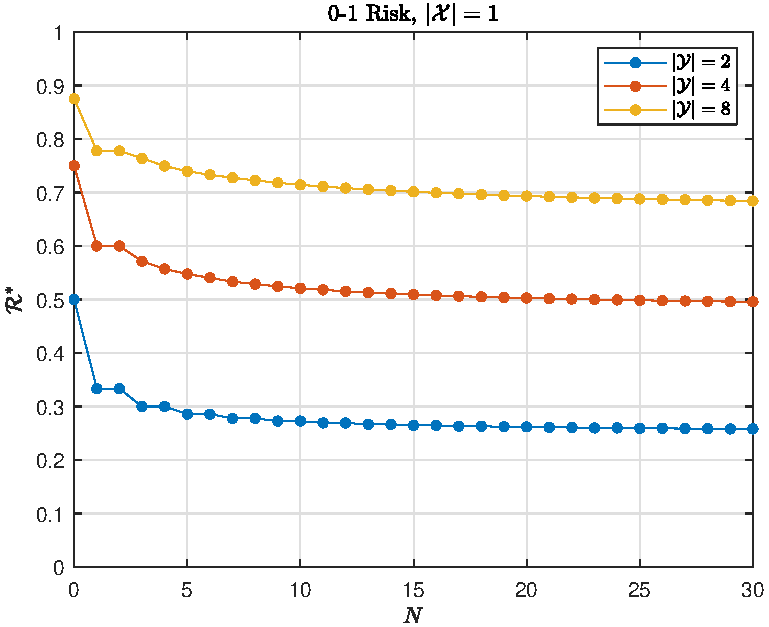
\includegraphics[width=0.7\linewidth]{Risk_01_uni_N_leg_My.pdf}
\caption{Minimum 0-1 Risk vs training set volume $N$}
\label{fig:Risk_01_uni_N_leg_My}
\end{figure}

\begin{figure}
\centering
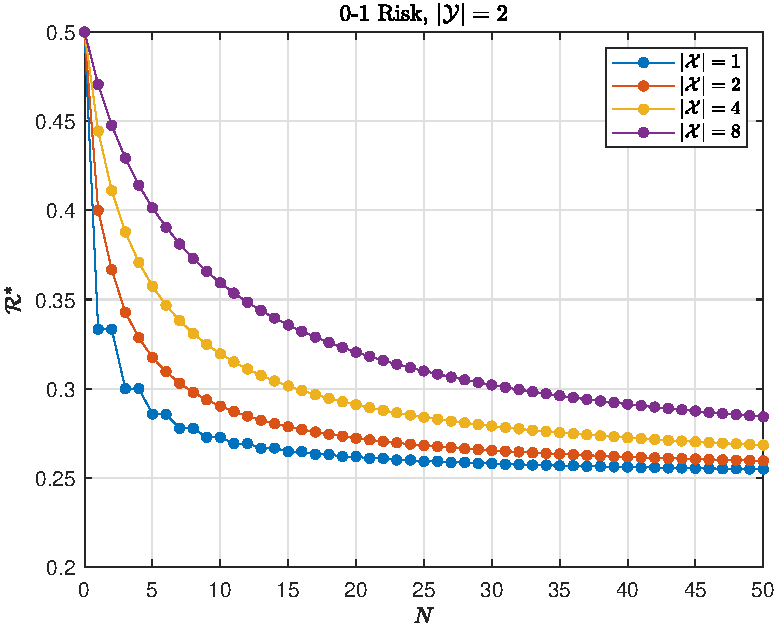
\includegraphics[width=0.7\linewidth]{Risk_01_uni_N_leg_Mx.pdf}
\caption{Minimum 0-1 Risk vs training set volume $N$}
\label{fig:Risk_01_uni_N_leg_Mx}
\end{figure}

Further insight into how $|\Xcal|$ affects the risk can be acquired by plotting the risk as a function of $N/|\Xcal|$. In Figure \ref{fig:Risk_01_uni_N-Mx}, it is shown that the minimal risk can be approximated by a function dependent only on $N/|\Xcal|$; of the series plotted, only the series for $|\Xcal| = 1$ shows notable non-negligible from the others.

\begin{figure}
\centering
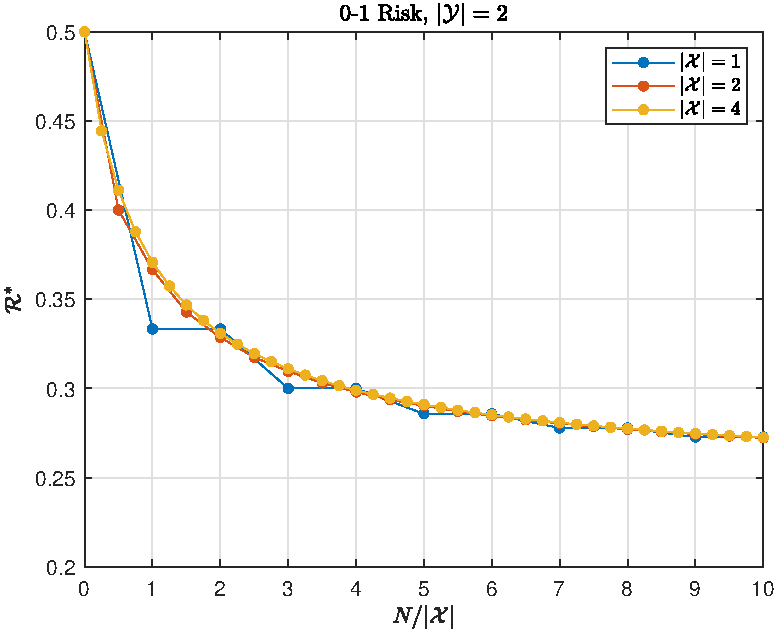
\includegraphics[width=0.7\linewidth]{Risk_01_uni_N-Mx.pdf}
\caption{Minimum 0-1 Risk vs $N/|\Xcal|$}
\label{fig:Risk_01_uni_N-Mx}
\end{figure}


It is also useful to graph the $N=0$ and $N \to \infty$ minimum risk as a function of $|\Ycal|$; both formulas are independent of $|\Xcal|$. Figure \ref{fig:Risk_01_uni_N_bounds} displays these bounds; note the margin in the probability of error between the optimal $N=0$ and $N \to \infty$ classifiers. For $|\Ycal| = 2$ binary classification, both sequences are at their minimum and infinite training data provides a reduction in expected probability of error from 0.5 to 0.25. As $|\Ycal|$ increases, the classification risk for both the $N=0$ and $N \to \infty$ cases tend to unity and the error reduction for $N \to \infty$ decreases. 





\begin{figure}
\centering
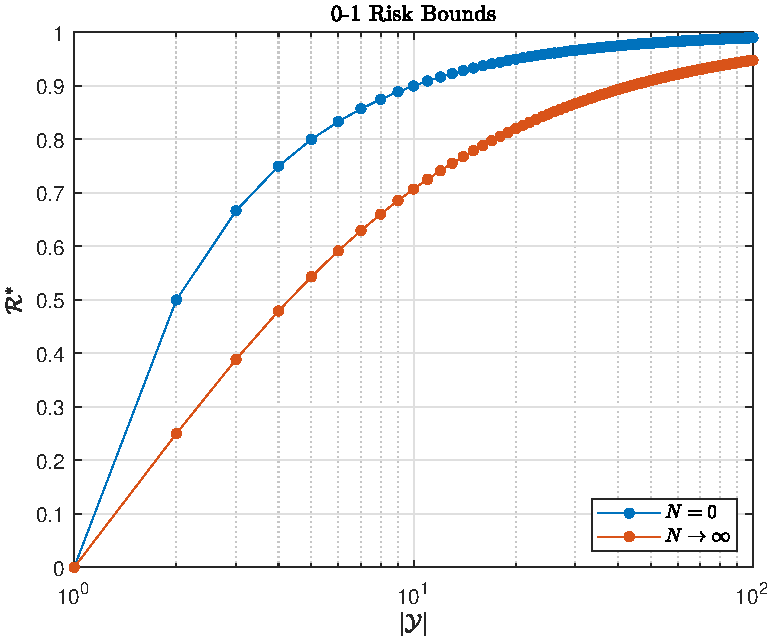
\includegraphics[width=0.7\linewidth]{Risk_01_uni_N_bounds.pdf}
\caption{Minimum 0-1 Risk vs $|\Ycal|$}
\label{fig:Risk_01_uni_N_bounds}
\end{figure}




\newpage
PGR: newpage

\subsubsection{Conditional Probability of Error for a Dirichlet-based Classifier}

PGR: INCOMPLETE

PGR: comment on alpha0 versus alphax simplification


Substituting the optimal Dirichlet-based classifier into the formula for the conditional probability of error \eqref{eq:risk_cond_01}, the risk is
\begin{IEEEeqnarray}{rCl}
\Rcal_{\Theta}(f ; \uptheta) & = & 1 - \sum_{x \in \Xcal} \upthetam(x) \Erm_{\uppsi | \upthetam,\upthetac} \bigg[ \upthetac\Big( \argmax_{y \in \Ycal} \big( N \uppsi(y,x) + \alpha_0 \alpha(y,x) \big) ;x \Big) \bigg] \;.
\end{IEEEeqnarray}
Figures \ref{fig:Risk_cond_01_Dir_N_leg_a0__subj_good} and \ref{fig:Risk_cond_01_Dir_N_leg_a0__subj_bad} show how the conditional risk trends for classifiers based on well-matched and poorly-matched informative Dirichlet priors, respectively. Note that the well-matched prior does better with higher prior concentrations $\alpha_0$; this is reflective of the fact that the maximizing arguments $y \in \Ycal$ of both the true model $\thetac(x)$ and the prior mean $\alphac(x)$ are the same.
\begin{figure}
\centering
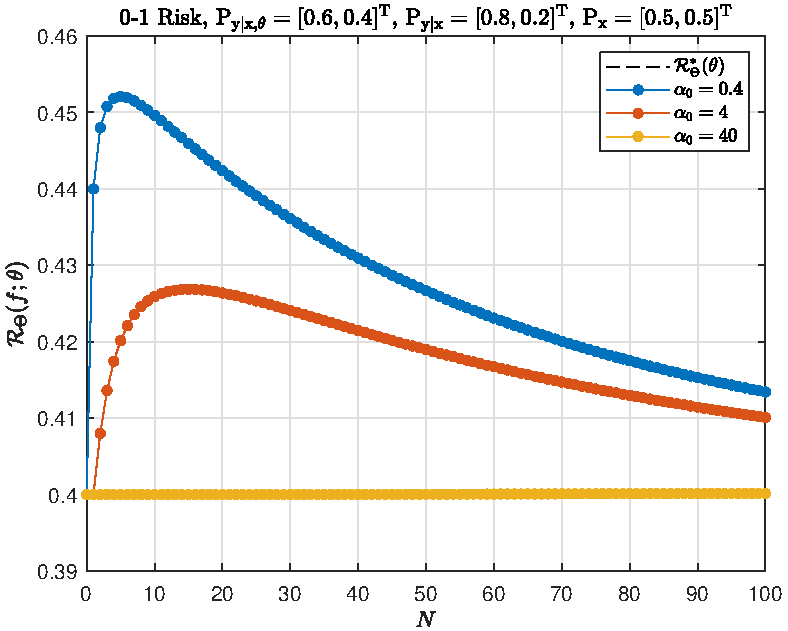
\includegraphics[width=0.7\linewidth]{Risk_cond_01_Dir_N_leg_a0__subj_good.pdf}
\caption{Excess conditional probability of error, well-matched informative Dirichlet-based classifier}
\label{fig:Risk_cond_01_Dir_N_leg_a0__subj_good}
\end{figure}
%
\begin{figure}
\centering
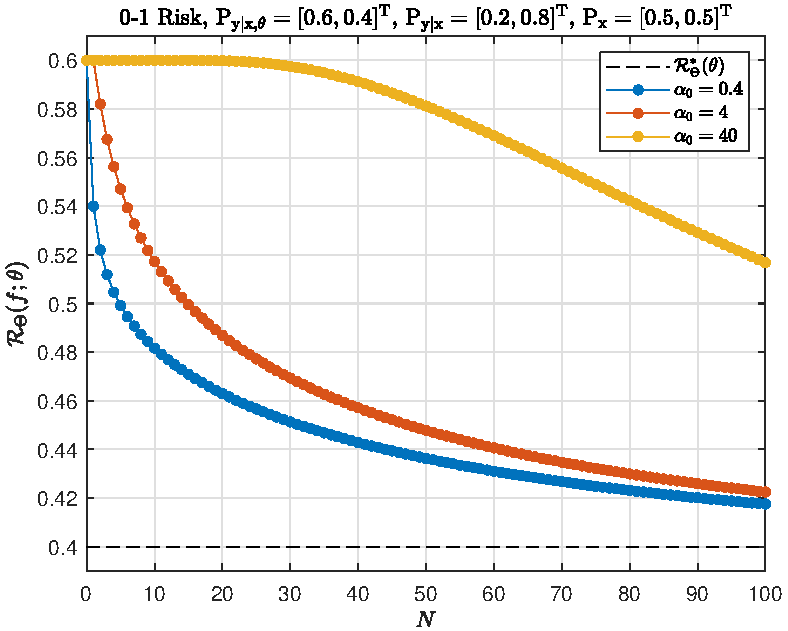
\includegraphics[width=0.7\linewidth]{Risk_cond_01_Dir_N_leg_a0__subj_bad.pdf}
\caption{Excess conditional probability of error, poorly-matched informative Dirichlet-based classifier}
\label{fig:Risk_cond_01_Dir_N_leg_a0__subj_bad}
\end{figure}

Also, it is important to consider how a given classifier performs for varying models $\thetac(x)$. Figures \ref{fig:Risk_cond_ex_01_Dir_theta__uni} and \ref{fig:Risk_cond_ex_01_Dir_theta__subj} demonstrate the excess conditional probability of error achieved by the conditional majority decision (based on a non-informative Dirichlet prior) and by a classifier derived from an informative Dirichlet prior, respectively. Note that while the former has fewer models for which the error is critically high, the latter has more models for which the clairvoyant risk $\Rcal_{\Theta}^*(\theta)$ is achieved. This a fundamental trade-off between Bayesian learners based on non-informative versus informative priors.
\begin{figure}
\centering
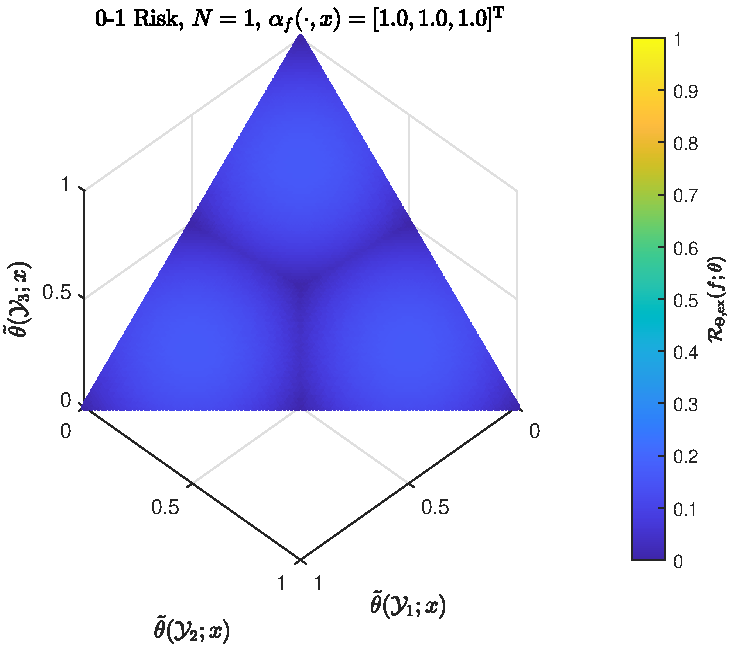
\includegraphics[width=0.7\linewidth]{Risk_cond_ex_01_Dir_theta__uni.pdf}
\caption{Excess conditional probability of error, conditional majority decision}
\label{fig:Risk_cond_ex_01_Dir_theta__uni}
\end{figure}
%
\begin{figure}
\centering
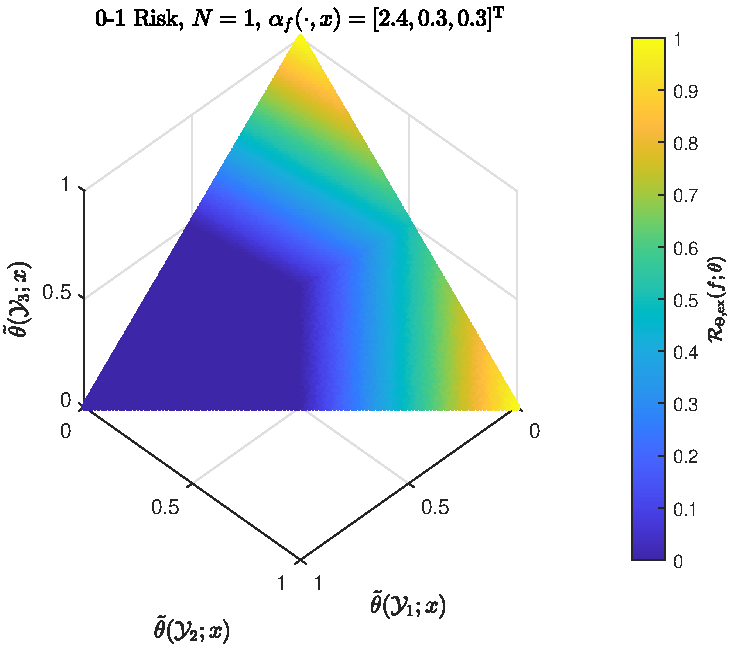
\includegraphics[width=0.7\linewidth]{Risk_cond_ex_01_Dir_theta__subj.pdf}
\caption{Excess conditional probability of error, informative Dirichlet-based classifier}
\label{fig:Risk_cond_ex_01_Dir_theta__subj}
\end{figure}































%\chapter{Extention to Infinite-Dimensional Spaces - Countably Infinite}
%
%\todohigh{DELETE or REWORK TO MERGE WITH FINITE Ch}
%
%\section{Intro}
%
%This chapter extends previous results for applications where the space $\Ycal$ is countably infinite, that is $|\Ycal| = \aleph_0$. Specifically, the model prior distribution will be characterized by a discrete-domain Dirichlet process.
%
%
%
%
%\section{Basic Model}
%
%
%\subsection{Probability Distributions}
%
%PGR: ???
%
%
%\subsubsection{Model PDF, $\prm_{\uptheta}(\theta)$}
%
%PGR: Valid model representation? Marginals instead?
%
%
%\begin{IEEEeqnarray}{rCl}
%\prm_{\uptheta}(\theta) & = & \beta(\alpha_0 \alpha)^{-1} \prod_{y \in \Ycal} \uptheta(y)^{\alpha(y) - 1} \;,
%\end{IEEEeqnarray}
%
%\begin{equation}
%\beta(\alpha_0 \alpha) = \frac{\prod_{y \in \Ycal} \Gamma\big( \alpha_0 \alpha(y) \big)}{\Gamma \left( \sum_{y \in \Ycal} \alpha(y) \right)} \;.
%\end{equation}
%
%The first and second joint moments of the model are 
%\begin{equation}
%\mu_{\uptheta}(y) = \Erm_{\uptheta}\big[ \uptheta(y) \big] = \frac{\alpha(y)}{\alpha_0}
%\end{equation}
%and
%\begin{IEEEeqnarray}{rCl}
%\Erm_{\uptheta}\big[ \uptheta(y) \uptheta(y') \big] & = & \frac{\alpha(y) \alpha(y') + \alpha(y) \delta[y,y']}{\alpha_0 (\alpha_0+1)} \;.
%\end{IEEEeqnarray}
%
%
%
%
%\subsubsection{Training Data PMF, $\Prm_{\Drm}$}
%
%\begin{equation}
%\Prm(\Drm | \uptheta) = \prod_{y \in \Ycal} \uptheta(y)^{\Psi(y;\Drm)} \;.
%\end{equation}
%
%\begin{equation}
%\Prm(\uppsi | \uptheta) = \Mcal(\uppsi) \prod_{y \in \Ycal} \uptheta(y)^{\uppsi(y)} \;,
%\end{equation}
%
%Thus,
%\begin{IEEEeqnarray}{rCl}
%\Prm(\uppsi) & = & \Mcal(\uppsi) \beta(\alpha_0 \alpha)^{-1} \beta(\alpha + \uppsi) \;.
%\end{IEEEeqnarray}
%
%The first and second joint moments of $\uppsi$ are
%\begin{equation}
%\Erm_{\uppsi}\big[ \uppsi(y) \big] = N \frac{\alpha(y)}{\alpha_0}
%\end{equation}
%and
%\begin{equation}
%\Erm_{\uppsi}\big[ \uppsi(y) \uppsi(y') \big] 
%= \frac{N}{\alpha_0 (\alpha_0+1)} \big( (\alpha_0 + N)\alpha(y) \delta[y,y'] + (N-1) \alpha(y) \alpha(y') \big) \;.
%\end{equation}
%
%Also,
%\begin{equation}
%\Prm(\Drm) = \beta(\alpha_0 \alpha)^{-1} \beta \big( \alpha + \Psi(\Drm) \big) \;.
%\end{equation}
%
%
%
%
%
%
%\subsubsection{Output conditional PMF, $\Prm(\yrm | \Drm)$}
%
%\begin{IEEEeqnarray}{rCL}
%\prm(\uptheta | \Drm) & = & \frac{\Prm(\Drm | \uptheta) \prm_{\uptheta}(\theta)}{\Prm(\Drm)} \\
%& = & \beta \left( \alpha + \Psi(\Drm) \right)^{-1} \prod_{y \in \Ycal} \uptheta(y)^{\alpha(y) + \Psi(y;\Drm) - 1} \nonumber 
%\end{IEEEeqnarray}
%
%\begin{IEEEeqnarray}{rCL}
%\prm(\theta | \uppsi) = \beta \left( \alpha + \uppsi \right)^{-1} 
%\prod_{y \in \Ycal} \uptheta(y)^{\alpha(y) + \uppsi(y) - 1} \;,
%\end{IEEEeqnarray}
%
%The PMF of interest is
%\begin{IEEEeqnarray}{rCl}
%\Prm(\yrm | \Drm) & = & \Erm_{\uptheta | \Drm}\big[ \theta(\yrm) \big] \\
%& = & \frac{\alpha(\yrm) + \Psi(\yrm;\Drm)}{\alpha_0 + N} \nonumber \\
%& = & \left(\frac{\alpha_0}{\alpha_0+N}\right) \frac{\alpha(\yrm)}{\alpha_0} + \left(\frac{N}{\alpha_0+N}\right) \frac{\Psi(\yrm;\Drm)}{N} \nonumber
%\end{IEEEeqnarray}
%
%\begin{IEEEeqnarray}{rCl}
%\Prm(\yrm | \uppsi) & = & \Erm_{\theta | \uppsi} \big[ \theta(\yrm) | \uppsi \big] \\
%& = & \frac{\alpha(\yrm) + \uppsi(\yrm)}{\alpha_0 + N} \nonumber \\
%& = & \left(\frac{\alpha_0}{\alpha_0+N}\right) \frac{\alpha(\yrm)}{\alpha_0} + \left(\frac{N}{\alpha_0+N}\right) \frac{\uppsi(\yrm)}{N} \nonumber
%\end{IEEEeqnarray}
%
%
%
%\section{Application to Common Loss Functions}
%
%PGR: Definitely regression. Classification sensible for countably infinite?
%
%PGR: Results identical to finite Dirichlet
%
%\begin{IEEEeqnarray}{L}
%\Erm_{\yrm | \Drm} \big[ \Lcal(h,\yrm) \big] = \sum_{y \in \Ycal} \Lcal(h,y) \Prm_{\yrm | \Drm}(y | \Drm) \\
%= \frac{\sum_{y \in \Ycal} \alpha(y) \Lcal(h,y) + \sum_{y \in \Ycal} \Psi(y;\Drm) \Lcal(h,y)}{\alpha_0+N} \nonumber \\
%= \frac{\sum_{y \in \Ycal} \alpha(y) \Lcal(h,y) + \sum_{n=1}^N \Lcal\big( h,\Drm_n \big)}{\alpha_0+N} \nonumber \\
%= \left( \frac{\alpha_0}{\alpha_0+N} \right) \sum_{y \in \Ycal} \Lcal(h,y) \frac{\alpha(y)}{\alpha_0} +  \left( \frac{N}{\alpha_0+N} \right) N^{-1} \sum_{n=1}^N \Lcal\big( h,\Drm_n \big) \nonumber \;.
%\end{IEEEeqnarray}
%
%
%\section{General Model}
%
%Extension to output and input spaces $\Ycal$ and $\Xcal$ can have an infinite number of elements. 
%
%
%\section{Applications: General Model}
%
%PGR: Definitely regression. Classification sensible for countably infinite?
%
%PGR: Results identical to finite Dirichlet















\chapter{Continuous-Domain Dirichlet Model}

PGR: SPECIFY EUCLIDEAN/HILBERT??

PGR: account for impulsive alpha?

\todohi{discuss otimes for dirac, USE?}

This chapter extends further to the case where $\Ycal$ and $\Xcal$ are continuous spaces and the model $\uptheta$ is a continuous-domain random process. Note that $|\Ycal| \geq \aleph_1$ and $|\Xcal| \geq \aleph_1$. 


\section{Problem PGR MOD?}

\todohigh{LOCATION?? Up front?}

\subsection{Model}

The model $\uptheta$ is a PDF and has a continuous domain. Thus, the marginal model is defined as $\upthetam \equiv \int_{\Ycal} \uptheta(y,\cdot) {\drm}y \in \Pcal(\Xcal)$. 


\subsection{Empirical Sufficient Statistic}

The training data is distributed as 
\begin{IEEEeqnarray}{rCl}
\prm_{\Drm | \uptheta}\big( D | \theta \big) & = & \prod_{n=1}^N \prm_{\Drm_n | \uptheta}\big( D_n | \theta \big) = \prod_{n=1}^N \theta(D_n) \nonumber \\ 
& = & \exp\left( \sum_{n=1}^N \ln\big(\theta(D_n)\big) \right) \nonumber \\
& = & \exp\left( \int_{\Ycal \times \Xcal} N \Psi(y,x;D) \ln\big(\theta(y,x)\big) {\drm}y {\drm}x \right) \nonumber \\
& \equiv & \prod_{\Ycal \times \Xcal} \left( \theta(y,x)^{N \Psi(y,x;D)} \right)^{{\drm}y {\drm}x} \;,
\end{IEEEeqnarray}
where the operator $\prod$ is the geometric integral, the continuous analog of the discrete product operator.

\todohigh{CITE for geometric integral!!}

Note that the dependency on the training data is expressed via the empirical transform $\Psi : \Dcal \mapsto \Uppsi \subset \Uptheta$, redefined for continuous data as
\begin{IEEEeqnarray}{rCl}
\Psi(D) & = & \frac{1}{N} \sum_{n=1}^N \delta \big( \cdot - D_n \big) \\
& \equiv & \frac{1}{N} \sum_{n=1}^N \delta(\cdot - Y_n) \delta(\cdot - X_n) ?? \nonumber \;.
\end{IEEEeqnarray}
Define the new random process $\uppsi \equiv \Psi(\Drm) \in \Uppsi$. Since the likelihood function only depends on the data through $\Psi(\Drm)$, the distribution $\prm_{\Drm | \uppsi,\uptheta}$ is uniform on the discrete set $\{D \in \Dcal : \Uppsi(D) = \uppsi\}$; consequently, the empirical model $\uppsi$ is a sufficient statistic.

\todomid{PDF for psi using geometric integral for Mcal?}

As shown in Appendix \ref{app:EP}, given $\uptheta$, the empirical model is a continuous-domain empirical process $\uppsi \sim \EP(N,\theta)$. The first and second joint moments are
\begin{IEEEeqnarray}{rCl}
\mu_{\uppsi | \uptheta} & = & \uptheta
\end{IEEEeqnarray}
and
\begin{IEEEeqnarray}{L}
\Erm_{\uppsi | \uptheta}\big[ \uppsi(y,x) \uppsi(y',x') \big] \\
\quad = \frac{1}{N} \uptheta(y,x) \delta(y - y') \delta(x - x') + \left(1 - \frac{1}{N}\right) \uptheta(y,x) \uptheta(y',x') \nonumber
\end{IEEEeqnarray}
and the covariance function is
\begin{IEEEeqnarray}{rCl}
\Sigma_{\uppsi | \uptheta}(y,x,y',x' | \theta) & = & \frac{1}{N} \big( \theta(y,x) \delta(y - y') \delta(x - x') - \theta(y,x) \theta(y',x') \big) \;.
\end{IEEEeqnarray}




\subsubsection{Marginal and Conditional Data Distributions}

The marginal and conditional distributions of the data using the representation $\Drm \Leftrightarrow (\Yrm,\Xrm)$ is of use.

The dependency of
\begin{IEEEeqnarray}{rCl}
\prm_{\Xrm | \uptheta}\big( X | \theta \big) & \equiv & \prod_{n=1}^N \prm_{\Xrm_n | \upthetam}\big( X_n | \thetam \big) = \prod_{n=1}^N \thetam(X_n) \nonumber \\ 
& = & \prod_{\Xcal} \left( \thetam(x)^{N \Psim(x;X)} \right)^{{\drm}x} \;,
\end{IEEEeqnarray}
on $X$ is expressed via the marginal empirical statistic $\Psim : \Xcal^N \mapsto \Uppsim \subset \Pcal(\Xcal)$, defined as
\begin{IEEEeqnarray}{rCl}
\Psim(X) & = & \frac{1}{N} \sum_{n=1}^N \delta\big( \cdot - X_n \big) = \int_{\Ycal} \Psi(y,\cdot;D) {\drm}y \;.
\end{IEEEeqnarray}
Note that the dependency on $\uptheta$ is only through the marginal model $\upthetam$.

The conditional distribution of the values $\Yrm$ given the corresponding $\Xrm$ and the model $\uptheta$,
\begin{IEEEeqnarray}{rCl}
\prm_{\Yrm | \Xrm,\uptheta}\big( Y | X,\theta \big) & = & \prod_{n=1}^N \frac{\prm_{\Yrm_n,\Xrm_n | \uptheta}\big( Y_n,X_n | \theta \big)}{\prm_{\Xrm_n | \uptheta}\big( X_n | \theta \big)} = \prod_{n=1}^N \thetac(Y_n;X_n) \nonumber \\
& = & \prod_{\Xcal} \left( \prod_{\Ycal} \thetac(y;x)^{\Psic(y;x;Y,X) {\drm}y} \right)^{N \Psim(x;X) {\drm}x} 
\end{IEEEeqnarray}
depends only on the conditional models $\upthetac(x)$. The dependency on the data $\Drm$ can be expressed using $\Psim$ and $\Psic : \{\Ycal \times \Xcal\}^N \mapsto \Uppsic \subset \Pcal(\Ycal)^{\Xcal}$, defined as
\begin{equation}
\Psic(x;Y,X) = \frac{\Psi(\cdot,x;Y,X)}{\Psim(x;X)} = \frac{\sum_{n=1}^N \delta\big( \cdot - Y_n \big) \delta\big[ x,X_n \big]}{\sum_{n=1}^N \delta\big[ x,X_n \big]} \;.
\end{equation}


The same bijection can be used to decompose the empirical process into marginal and conditional empirical processes. The ``marginalized'' random process $\uppsim \in \Uppsim \subset \Pcal(\Xcal)$ is now defined as $\uppsim \equiv \int_{\Ycal} \uppsi(y,\cdot) {\drm}y$. Using the aggregation property of empirical processes detailed in Appendix \ref{app:EP}, it can be shown that conditioned on the model $\uptheta$, the marginal model is also an Empirical process, $\uppsim | \upthetam \sim \EP(N,\upthetam)$. Note the conditional independence from $\upthetac$. 

Additionally, given the model $\uptheta$, the conditional processes $\uppsic \in \Uppsic$ are independent Empirical processes $\uppsic(x) | \uppsim(x),\upthetac(x) \sim \EP\big( \delta(0)^{-1} N \uppsim(x),\upthetac(x) \big)$. They are independent of the marginal model $\upthetam$.

\todohigh{delta domain? dx?}










\section{Probability Distributions}


\subsection{Model $\uptheta$ Characterization}

The model is characterized by a Dirichlet process $\uptheta \sim \DP(\alpha_0, \alpha)$ with concentration $\alpha_0$ and mean function $\alpha \in \Pcal(\Ycal \times \Xcal)$. As shown in Appendix \ref{app:DP}, the expected value of a Dirichlet process is $\DP(\alpha_0, \alpha)$
\begin{equation}
\mu_{\uptheta} = \alpha
\end{equation}
and the correlation function is
\begin{IEEEeqnarray}{rCl}
\Erm_{\uptheta}\big[ \uptheta(y,x) \uptheta(y',x') \big] & = & \frac{\alpha(y,x) \delta(y-y')\delta(x-x') + \alpha_0 \alpha(y,x) \alpha(y',x')}{\alpha_0+1} \\
& = & \frac{1}{\alpha_0+1} \alpha(y,x) \delta(y-y')\delta(x-x') + \frac{\alpha_0}{\alpha_0+1} \alpha(y,x) \alpha(y',x') \nonumber \;.
\end{IEEEeqnarray}
The covariance function is thus
\begin{IEEEeqnarray}{rCl}
\Sigma_{\uptheta}(y,x,y',x') \big] & = & \frac{\alpha(y,x) \delta(y-y')\delta(x-x') - \alpha(y,x) \alpha(y',x')}{\alpha_0+1} \;.
\end{IEEEeqnarray}


\subsubsection{Marginal and Conditional Distributions}

The marginal distribution $\upthetam$ and the conditional distribution $\upthetac$ are also of interest. Define the bijection $\alpha \Leftrightarrow (\alpham,\alphac)$, where $\alpham \equiv \int_{\Ycal} \alpha(y,\cdot) {\drm}y$ (and $\alphac(x) \equiv \alpha(\cdot,x) / \alpham(x)$) for each $x \in \Xcal$. Again, $\alpham \in \Pcal(\Xcal)$ and $\alphac \in \Pcal(\Ycal)^{\Xcal}$.

By the continuous-domain Dirichlet process properties detailed in Appendix \ref{app:DP}, $\upthetam \sim \DP(\alpha_0,\alpham)$ is a Dirichlet random process parameterized by concentration $\alpha_0$ and distribution $\alpham$; observe that the PDF $\prm_{\xrm} = \mu_{\upthetam} = \alpham$. Also, the functions $\upthetac(x) \sim \DP\big(\delta(0)^{-1} \alpha_0 \alpham(x), \alphac(x)\big)$ are independent Dirichlet processes and are independent of $\upthetam$ as well. Note that $\prm_{\yrm | \xrm} = \mu_{\upthetac}(\xrm) = \alphac(\xrm)$. 




\subsection{Predictive PDF, $\prm_{\yrm | \xrm,\Drm}$}

By the properties of the Dirichlet process proven in Appendix \ref{app:DP_post}, the model conditioned on the training data $\Drm$ is Dirichlet with concentration $\alpha_0 + N$ and mean function 
\begin{IEEEeqnarray}{rCl}
\mu_{\uptheta | \Drm} & = & \gamma \alpha + (1-\gamma) \Psi(\Drm) \;,
\end{IEEEeqnarray}
where $\Psi(y,x;D) = N^{-1} \sum_{n=1}^N \delta\big( (y,x) - D_n \big)$. 

Recall that $\Drm_n \Leftrightarrow \big( \Yrm_n,\Xrm_n \big)$, where $\Yrm \in \Ycal^N$ and $\Xrm \in \Xcal^N$. Since $\prm_{\yrm,\xrm | \Drm} = \mu_{\uptheta | \Drm}$, by Bayes rule the marginal PDF is
\begin{IEEEeqnarray}{rCl}
\prm_{\xrm | \Drm} \equiv \prm_{\xrm | \Xrm} & = & \gamma \alpham + (1-\gamma) \Psim(\Xrm) \;,
\end{IEEEeqnarray}
and the conditional PDF of interest is
\begin{IEEEeqnarray}{rCl}
\prm_{\yrm | \xrm,\Drm} & = & \frac{\alpha_0 \alpha(\cdot,\xrm) + N \Psi(\cdot,\xrm;\Drm)}{\alpha_0 \alpham(\xrm) + N \Psim(\xrm;\Drm)} \\
& \equiv & \frac{\alpha_0 \alpha(\cdot,\xrm) + \sum_{n=1}^N \delta\big( \cdot - \Yrm_n \big) \delta\big( \xrm - \Xrm_n \big)}{\alpha_0 \alpham(\xrm) + \sum_{n=1}^N \delta\big( \xrm - \Xrm_n \big)} \nonumber \\
& = & \left(\frac{\alpha_0 \alpham(\xrm)}{\alpha_0 \alpham(\xrm)+N \Psim(\xrm;\Drm)}\right) \alphac(\xrm) + \left(\frac{N \Psim(\xrm;\Drm)}{\alpha_0 \alpham(\xrm)+N \Psim(\xrm;\Drm)}\right) \Psic(\xrm;\Drm) \nonumber \\
& = & \gammam(\xrm; \Drm) \alphac(\xrm) + \big(1 - \gammam(\xrm; \Drm)\big) \Psic(\xrm;\Drm) \nonumber \;.
\end{IEEEeqnarray}


The conditional distribution when $\Xcal$ is a continuous space has notable differences from its form for a countable set $\Xcal$. Specifically, since $\Psim(x;D)$ is either zero or tends towards infinity, an upper-bounded prior mean $\alpha$ will result in convex coefficients that are zero or one, just as for the discrete-domain PMF for $\alpha_0 \to 0$. In this case, the distribution for a given observation $\xrm$ will be either strictly dependent on either the training data or the prior knowledge; if any training data are observed satisfying $\Xrm_n = \xrm$, then the conditional empirical model will be used for prediction.



\subsubsection{Via the Conditional Model Process}

As the Dirichlet prior implies that $\upthetam$ is independent from $\upthetac$, the likelihood $\prm_{\Drm | \upthetam}$ is proportionate to $\prm_{\Xrm | \upthetam} = \bigotimes_{n=1}^N \upthetam$. Thus, using the properties detailed in Appendix \ref{app:DP_post}, it can be shown that the marginal process satisfies $\upthetam | \Drm \sim \upthetam | \Xrm \sim \DP(\alpha_0 + N, \mu_{\upthetam | \Xrm})$, where
\begin{IEEEeqnarray}{rCl}
\mu_{\upthetam | \Xrm} & = & \gamma \alpham + (1-\gamma) \Psim(\Xrm) \;.
\end{IEEEeqnarray}

Similarly, using the empirical statistic representation, the model likelihood of $\uppsic,\uppsim | \upthetam$ is proportionate to $\uppsim | \upthetam \sim \EP(N,\upthetam)$. As a result, observe that $\upthetam | \uppsim,\uppsic \sim \upthetam | \uppsim \sim \DP(\alpha_0 + N, \mu_{\upthetam | \uppsim})$, where
\begin{IEEEeqnarray}{rCl}
\mu_{\upthetam | \uppsim} & = & \gamma \alpham + (1-\gamma) \uppsim \;.
\end{IEEEeqnarray}
Recall that $\prm_{\xrm | \uppsi} \equiv \mu_{\upthetam | \uppsim}$.


The independence of the marginal and conditional models also implies that the likelihood $\prm_{\xrm,\Drm | \upthetac}$ is proportionate to $\prm_{\Yrm | \Xrm,\upthetac} = \bigotimes_{n=1}^N \upthetac(\Xrm_n)$. Thus, it can be shown that $\upthetac(x) | \xrm,\Drm \sim \upthetac(x) | \Drm \sim \DP\Big(\delta(0)^{-1} \big(\alpha_0 \alpham(x) + N \Psim(x;\Drm) \big), \mu_{\upthetac(x) | \Drm} \Big)$, where
\begin{IEEEeqnarray}{rCl}
\mu_{\upthetac(x) | \Drm} & = & \gammam(\xrm; \Drm) \alphac(x) + \big(1 - \gammam(\xrm; \Drm)\big) \Psic(x;\Drm) \nonumber \;.
\end{IEEEeqnarray}

Similarly, using the empirical statistic representation, the likelihood of $\xrm,\uppsic,\uppsim | \upthetac$ is proportionate to $\uppsic | \uppsim, \upthetam \sim \bigotimes_{x \in \Xcal} \EP(N \uppsim(x), \upthetac(x))$. Consequently, observe that $\upthetac(x) | \xrm,\uppsim,\uppsic \sim \upthetac(x) | \uppsim(x),\uppsic(x) \sim \DP\Big( \delta(0)^{-1} \big(\alpha_0 \alpham(x) + N \uppsim(x) \big), \mu_{\upthetac(x) | \uppsim(x),\uppsic(x)} \Big)$, where
\begin{IEEEeqnarray}{rCl}
\mu_{\upthetac(x) | \uppsim(x),\uppsic(x)} & = & \gammam(\xrm; \uppsim) \alphac(x) + \big(1 - \gammam(\xrm; \uppsim)\big) \uppsic(x) \nonumber \;.
\end{IEEEeqnarray}
Recall that $\prm_{\yrm | \xrm,\uppsi}(x, \psi) \equiv \mu_{\upthetac(x) | \uppsim(x),\uppsic(x)}\big( \psim(x), \psic(x) \big)$.


\todomid{sim, otimes notation??}




\subsection{Training Data PDF, $\prm_{\Drm}$}

\todohi{move before predictive}

\todolo{geometric integral beta function??}

Using the Dirichlet process properties shown in Appendix \ref{app:DP},
\begin{IEEEeqnarray}{rCl}
\prm_{\Drm_{n+1} | \Drm_n,\ldots,\Drm_1} & = & \mu_{\uptheta | \Drm_n,\ldots,\Drm_1} \\
& \equiv & \frac{\alpha_0 \alpha + \sum_{i=1}^n \delta\big( \cdot - \Yrm_i \big) \delta\big( \cdot - \Xrm_i \big)}{\alpha_0 + n} \nonumber
\end{IEEEeqnarray}
and thus the training data PDF is
\begin{IEEEeqnarray}{rCl}
\prm_{\Drm}(D) & = & \Erm_{\uptheta}\left[ \prod_{n=1}^N \uptheta\big( D_n \big) \right] \\
& = & \prm_{\Drm_1}\big(D_1\big) \prod_{n=2}^N \prm_{\Drm_{n} | \Drm_{n-1},\ldots,\Drm_1}\big( D_n | D_{n-1},\ldots,D_1 \big) \nonumber \\
& \equiv & \alpha\big( Y_1,X_1 \big) \prod_{n=2}^N \frac{\alpha_0 \alpha\big( Y_n,X_n \big) + \sum_{i=1}^{n-1} \delta\big( Y_n -  Y_i \big) \delta\big( X_n - X_i \big)}{\alpha_0+n-1} \nonumber \;.
\end{IEEEeqnarray}


PGR: BELOW, just integrate??

It is instructional to find the PDF's for the training output values $\Yrm$ given the input values $\Xrm$, as well as the marginal PDF for the input values alone. Observe that since the independent observations $\Xrm_n | \upthetam$ are characterized by the Dirichlet process $\upthetam \sim \DP(\alpha_0,\alpham)$, the PDF for $\Xrm$ can be represented as
\begin{IEEEeqnarray}{rCl}
\prm_{\Xrm}(X) & = & \Erm_{\uptheta}\big[ \prm_{\Xrm | \uptheta}(X | \uptheta) \big] \equiv \Erm_{\upthetam}\left[ \prod_{n=1}^N \upthetam\big( X_n \big) \right] \\
& = & \alpham\big( X_1 \big) \prod_{n=2}^N \frac{\alpha_0 \alpham\big( X_n \big) + \sum_{i=1}^{n-1} \delta\big( X_n-X_i \big)}{\alpha_0+n-1} \nonumber \;.
\end{IEEEeqnarray}
Note that the marginal PDF's are $\prm_{\Xrm_n} = \prm_{\xrm} = \mu_{\upthetam} = \alpham$.

%The PDF for $\Xrm$ is
%\begin{IEEEeqnarray}{rCl}
%\prm(X) & = & \int_{Y(1)} {\drm}Y(1) \ldots \int_{Y(N)} {\drm}Y(N) \frac{\alpha(Y(1),X(1))}{\alpha_0} \\
%&& \quad \prod_{n=2}^N \frac{\alpha(Y_n,X_n) + \sum_{i=1}^{n-1} \delta(Y_n-Y(i)) \delta(X_n-X(i))}{\alpha_0+n-1} \\
%& = & \int_{Y(1)} {\drm}Y(1) \ldots \int_{Y(N-1)} {\drm}Y(N-1) \frac{\alpha(Y(1),X(1))}{\alpha_0} \\
%&& \quad \prod_{n=2}^{N-1} \frac{\alpha(Y_n,X_n) + \sum_{i=1}^{n-1} \delta(Y_n-Y(i)) \delta(X_n-X(i))}{\alpha_0+n-1} \\
%&& \qquad \frac{\alpha'(X(N)) + \sum_{i=1}^{N-1} \delta(X(N)-X(i))}{\alpha_0+N-1} \\
%& = & \ldots \\
%& = & \frac{\alpha'(X(1))}{\alpha_0} \prod_{n=2}^N \frac{\alpha'(X_n) + \sum_{i=1}^{n-1} \delta(X_n-X(i))}{\alpha_0+n-1}
%\end{IEEEeqnarray}



Using Bayes theorem,
\begin{IEEEeqnarray}{rCl}
\prm_{\Yrm | \Xrm}(Y | X) & = & \Erm_{\upthetac}\left[ \prod_{n=1}^N \upthetac\big( Y_n;X_n \big) \right] \\
& = & \alphac\big( Y_1;X_1 \big) \prod_{n=2}^N \frac{\alpha_0 \alpham(X_n) \alphac\big( Y_n;X_n \big) + \sum_{i=1}^{n-1} \delta\big( Y_n-Y_i \big) \delta\big( X_n-X_i \big)}{\alpha_0 \alpham\big( X_n \big) + \sum_{i=1}^{n-1} \delta\big( X_n-X_i \big)} 
\end{IEEEeqnarray}


\todomid{express conditional using Dir aggregation conditional independence properties?}


%Marginalized conditional PDF's for the first and second samples are found. Observe that the marginal distribution for the first $N-1$ values of $\Yrm$ is
%\begin{IEEEeqnarray}{L}
%\prm_{\Yrm_1,\ldots,\Yrm_{N-1} | \Xrm}\big( Y_1,\ldots,Y_{N-1} | X \big) \\
%= \int_{\Ycal} \frac{\alpha\big( Y_1,X_1 \big)}{\alpha'\big( X_1 \big)} \prod_{n=2}^N \frac{\alpha \big( Y_n,X_n \big) + \sum_{i=1}^{n-1} \delta\big( Y_n-Y_i \big) \delta\big( X_n-X_i \big)}{\alpham\big( X_n \big) + \sum_{i=1}^{n-1} \delta\big( X_n-X_i \big)} {\drm}Y_N \nonumber \\
%= \frac{\alpha\big( Y_1,X_1 \big)}{\alpha'\big( X_1 \big)} \prod_{n=2}^{N-1} \frac{\alpha\big( Y_n,X_n \big) + \sum_{i=1}^{n-1} \delta\big( Y_n-Y_i \big) \delta\big( X_n-X_i \big)}{\alpham\big( X_n \big) + \sum_{i=1}^{n-1} \delta\big( X_n-X_i \big)} \nonumber
%\end{IEEEeqnarray}
%which is independent of $\Xrm_N$. Repeated integrations and an application of the permutation invariance principle can show that when conditioned on $\Xrm$ any subset of training data values $\Yrm_1,\ldots,\Yrm_N$ will only be dependent on the corresponding values $\Xrm_n$. 


Note that the independent observations $\Yrm_n | \Xrm_n,\upthetac$ are conditionally independent of $\Xrm_i$, $i \neq n$, and that they are characterized by the independent processes $\upthetac(x) \sim \DP\big(\delta(0)^{-1} \alpha_0 \alpham(x), \alphac(x)\big)$. Consequently, the joint distribution of any samples from $\Yrm$ given $\Xrm$ will only depend on the matching training samples.

The first and second order conditional distributions are of specific interest. The first order conditional distributions are
\begin{IEEEeqnarray}{rCl}
\prm_{\Yrm_n | \Xrm}(X) & = & \prm_{\Yrm_n | \Xrm_n}(X_n) = \prm_{\yrm | \xrm}(X_n) = \mu_{\upthetac(X_n)} = \alphac(X_n) \;,
\end{IEEEeqnarray}
To determine the second order conditional distributions, first note that for $\Xrm_n \neq \Xrm_{n'}$, $\prm_{\Yrm_n,\Yrm_{n'} | \Xrm_n,\Xrm_{n'}} = \mu_{\upthetac(\Xrm_n)} \otimes \mu_{\upthetac(\Xrm_{n'})} = \alphac(\Xrm_n) \otimes \alphac(\Xrm_{n'})$. Conversely, if $\Xrm_n = \Xrm_{n'}$, then
\begin{IEEEeqnarray}{L}
\prm_{\Yrm_n,\Yrm_{n'} | \Xrm_n,\Xrm_{n'}} = \Erm_{\upthetac(\Xrm_n)} \big[\upthetac(\Xrm_n) \otimes \upthetac(\Xrm_n)\big]  \\
\quad = \frac{\diag\big(\alphac(\Xrm_n)\big) + \delta(0)^{-1} \alpha_0 \alpham(\Xrm_n) \alphac(\Xrm_n) \otimes \alpha(\Xrm_n)}{\delta(0)^{-1} \alpha_0 \alpham(\Xrm_n) + 1} \nonumber \\
\quad = \frac{\delta(0)}{\alpha_0 \alpham(\Xrm_n) + \delta(0)} \diag\big(\alphac(\Xrm_n)\big) + \frac{\alpha_0 \alpham(\Xrm_n)}{\alpha_0 \alpham(\Xrm_n) + \delta(0)} \alphac(\Xrm_n) \otimes  \alpha(\Xrm_n) \nonumber \;.
\end{IEEEeqnarray}
Combining, the second order distribution formula is
\begin{IEEEeqnarray}{L}
\prm_{\Yrm_n,\Yrm_{n'} | \Xrm_n,\Xrm_{n'}} \\
\quad = \frac{\delta(\Xrm_n-\Xrm_{n'})}{\alpha_0 \alpham(\Xrm_n) + \delta(\Xrm_n-\Xrm_{n'})} \diag\big(\alphac(\Xrm_n)\big) + \frac{\alpha_0 \alpham(\Xrm_n)}{\alpha_0 \alpham(\Xrm_n) + \delta(\Xrm_n-\Xrm_{n'})} \alphac(\Xrm_n) \otimes \alpha(\Xrm_{n'}) \nonumber
\end{IEEEeqnarray}
%\begin{IEEEeqnarray}{L}
%\Prm_{\Yrm_n,\Yrm_{n'} | \Xrm_n,\Xrm_{n'}} (y,y' | x,x') \\
%\quad = \frac{\alpha_0 \alpham(x) \alphac(y;x) \alpha(y';x') + \alphac(y;x) \delta(y-y') \delta(x-x')}{\alpha_0 \alpham(x) + \delta(x-x')} \nonumber \\
%\quad = \frac{\delta(x-x')}{\alpha_0 \alpham(x) + \delta(x-x')} \alphac(y;x) \delta(y-y') + \frac{\alpha_0 \alpham(x)}{\alpha_0 \alpham(x) + \delta(x-x')} \alphac(y;x) \alpha(y';x') \nonumber
%\end{IEEEeqnarray}









PGR: Dirichlet-Empirical Process perspective

We have the Dirichlet-Empirical process $\uppsi \equiv \Psi(\Drm) \sim \DEP(N,\alpha_0,\alpha)$ with mean and correlation functions
\begin{IEEEeqnarray}{rCl}
\mu_{\uppsi} & = & \alpha 
\end{IEEEeqnarray}
and
\begin{IEEEeqnarray}{rCl}
\Erm_{\uppsi}\big[ \uppsi(y,x) \uppsi(y',x') \big] & = & \frac{\alpha_0^{-1} + N^{-1}}{1 + \alpha_0^{-1}} \alpha(y,x) \delta(y-y') \delta(x-x') \nonumber \\
&& \quad + \frac{1 - N^{-1}}{1 + \alpha_0^{-1}} \alpha(y,x) \alpha(y',x')
\end{IEEEeqnarray}
and covariance function
\begin{IEEEeqnarray}{rCl}
\Sigma_{\uppsi} & = & \frac{\alpha_0^{-1} + N^{-1}}{1 + \alpha_0^{-1}} \big( \diag(\alpha) - \alpha \otimes \alpha \big) \\
& = & \left(1 + \frac{\alpha_0}{N}\right) \Sigma_{\uptheta} \nonumber \;.
\end{IEEEeqnarray}

Observe that by the aggregation principle, $\uppsim \sim \DEP(N,\alpha_0,\alpham)$ is a DEP over the set $\Xcal$. Additionally, the 1-dimensional subsets conditioned on the marginalized DEP are characterized as
\begin{equation}
\uppsic(x) \big| \uppsim(x) \sim \DEP\left( \frac{N \uppsim(x)}{\delta(0)}, \frac{\alpha_0 \alpham(x)}{\delta(0)}, \alphac(x) \right)
\end{equation}











\section{Model Estimation Perspective} \label{sec:predictive_est_cont}


\begin{IEEEeqnarray}{L}
\Erm_{\uppsim,\uppsic | \upthetam,\upthetac}\big[ \Prm_{\yrm | \xrm,\uppsim,\uppsic} \big] 
\equiv \Erm_{\uppsim(\xrm),\uppsic(\xrm) | \upthetam(\xrm),\upthetac(\xrm)}\big[ \Prm_{\yrm | \xrm,\uppsim(\xrm),\uppsic(\xrm)} \big] \\ 
\quad = \Erm_{\uppsim(\xrm) | \upthetam(\xrm)} \big[\gammam(\xrm; \uppsim)\big] \alphac(\xrm) + \Erm_{\uppsim(\xrm) | \upthetam(\xrm)} \big[1 - \gammam(\xrm; \uppsim)\big] \upthetac(\xrm) \nonumber
\end{IEEEeqnarray}

To aid characterization of the estimator, define the random process $\Delta(\xrm;\uppsim,\uppsic,\upthetac) \equiv \prm_{\yrm | \xrm,\uppsim,\uppsic} - \prm_{\yrm | \xrm,\upthetac} \in \Rbb^{\Ycal}$. For a given $\xrm$, the bias of the conditional PDF estimate is
\begin{IEEEeqnarray}{rCl} \label{eq:predictive_bias_cont}
\mathrm{Bias}(\xrm;\upthetam,\upthetac) & = & \Erm_{\uppsim, \uppsic | \upthetam,\upthetac}\big[ \Delta(\xrm;\uppsim,\uppsic,\upthetac) \big] \\
& = & \Erm_{\uppsim(\xrm) | \upthetam(\xrm)}\big[\gammam(\xrm; \uppsim)\big] \big( \alphac(\xrm) - \upthetac(\xrm) \big) \nonumber
\end{IEEEeqnarray}
and its covariance function is 
\begin{IEEEeqnarray}{L} \label{eq:predictive_cov_cont}
\mathrm{Cov}(\xrm;\upthetam,\upthetac) = \Crm_{\uppsim,\uppsic | \upthetam,\upthetac} \big[\Prm_{\yrm | \xrm,\uppsim,\uppsic} \big] \\
\quad = \Erm_{\uppsim(\xrm) | \upthetam(\xrm)}\left[ \frac{\big(1 - \gammam(\xrm; \uppsim)\big)^2}{\delta(0)^{-1} N \uppsim(\xrm)} \right] \big( \diag\big(\upthetac(\xrm)\big) - \upthetac(\xrm) \otimes \upthetac(\xrm) \big) \nonumber \\
\qquad + \Crm_{\uppsim(\xrm) | \upthetam(\xrm)}\big[\gammam(\xrm; \uppsim)\big] \big( \alphac(\xrm) - \upthetac(\xrm) \big) \otimes \big( \alphac(\xrm) - \upthetac(\xrm) \big) \nonumber
\end{IEEEeqnarray}


\begin{IEEEeqnarray}{rCl} \label{eq:predictive_del_sq_cont}
\mathcal{E}(\xrm;\upthetam,\upthetac) & = & \Erm_{\uppsim,\uppsic | \upthetam,\upthetac} \Big[ \Delta(\xrm;\uppsim,\uppsic,\upthetac) \otimes \Delta(\xrm;\uppsim,\uppsic,\upthetac) \Big] \\
& = & \mathrm{Bias}(\xrm;\upthetam,\upthetac) \otimes \mathrm{Bias}(\xrm;\upthetam,\upthetac) + \mathrm{Cov}(\xrm;\upthetam,\upthetac) \nonumber \;.
\end{IEEEeqnarray}

Also of interest, the conditional expectation over $\xrm$ is
\begin{IEEEeqnarray}{L} \label{eq:predictive_E_del_sq_cont}
\Erm_{\xrm | \upthetam}\Big[ \mathcal{E}(\xrm;\upthetam,\upthetac) \Big] \\
\quad = \Erm_{\xrm | \upthetam}\left[ \Erm_{\uppsim(\xrm) | \upthetam(\xrm)}\big[ \gammam(\xrm; \uppsim)^2 \big] \big( \alphac(\xrm) - \upthetac(\xrm) \big) \otimes \big( \alphac(\xrm) - \upthetac(\xrm) \big)  \right] \nonumber \\
\qquad + \Erm_{\xrm | \upthetam}\left[ \Erm_{\uppsim(\xrm) | \upthetam(\xrm)}\left[ \frac{\big(1 - \gammam(\xrm; \uppsim)\big)^2}{\delta(0)^{-1} N \uppsim(\xrm)} \right] \Big( \diag\big(\upthetac(\xrm)\big) - \upthetac(\xrm) \otimes \upthetac(\xrm) \Big) \right] \nonumber \;.
\end{IEEEeqnarray}

Note that by the aggregation property of Empirical distributions, the empirical process $\uppsim(x)$ conditioned on the model $\upthetam(x)$ is distributed as
\begin{IEEEeqnarray}{rCl}
\prm_{\uppsim(x) | \upthetam(x)}\big(\psim(x) | \thetam(x) \big) & = & \Emp\Big( \big( \delta(0)^{-1} \psim(x),1 - \delta(0)^{-1} \psim(x)\big); N, \big( \delta(0)^{-1} \thetam(x), 1 - \delta(0)^{-1} \thetam(x)\big) \Big) \nonumber \\
& = & \Bi\big(\delta(0)^{-1} N \psim(x); N, \delta(0)^{-1} \thetam(x)\big) \;,
\end{IEEEeqnarray}
where $\Bi$ is the binomial PMF.



\todohigh{plots?}










\section{Applications: General Model}

\todohigh{Discuss overfitting, like discrete with infinite concentration}

PGR: COPIED, incomplete

\begin{IEEEeqnarray}{rCl}
\Erm_{\yrm | \xrm,\Drm} \big[ \Lcal(h,\yrm) \big] & = & \int_{\Ycal} \Lcal(h,y) \prm_{\yrm | \xrm,\Drm}(y | \xrm,\Drm) {\drm}y \\
& = & \gammam(\xrm; \Drm) \int_{\Ycal} \alphac(y;\xrm) \Lcal(h,y) {\drm}y \nonumber \\
&& \qquad + \big(1 - \gammam(\xrm; \Drm)\big) \int_{\Ycal} \Psic(y;\xrm;\Drm) \Lcal(h,y) {\drm}y \nonumber \\
& = & \left(\frac{\alpha_0 \alpham(\xrm)}{\alpha_0 \alpham(\xrm) + N \Psim(\xrm;\Drm)}\right) \Erm_{\yrm | \xrm}\big[ \Lcal(h,\yrm) \big] \nonumber \\
&& \qquad + \left(\frac{N \Psim(\xrm;\Drm)}{\alpha_0 \alpham(\xrm) + N \Psim(\xrm;\Drm)}\right) \frac{\sum_{n=1}^N \delta\big[\xrm, \Xrm_n\big] \Lcal\big( h,\Yrm_n \big)}{\sum_{n=1}^N \delta\big[\xrm, \Xrm_n\big]} \nonumber \;.
\end{IEEEeqnarray}



\subsection{Regression: the Squared-Error Loss}

\begin{equation}
\Lcal(h,y) = (h-y)^2 \;.
\end{equation}

Now we choose for the regression function to map to $\Hcal = \Ycal = \Rbb$.

\begin{IEEEeqnarray}{rCl}
\Rcal(f) & = & \Erm_{\uptheta} \Bigg[ \Erm_{\Drm | \uptheta} \bigg[ \Erm_{\yrm,\xrm | \uptheta} \Big[ \big( f( \xrm;\Drm)-\yrm \big)^2 \Big] \bigg] \Bigg] \\
& = & \Erm_{\xrm,\uptheta} \Big[ \Erm_{\yrm | \xrm,\uptheta} \big[ (\yrm - \mu_{\yrm | \xrm,\uptheta})^2 \big] \Big] + \Erm_{\uptheta} \bigg[ \Erm_{\xrm,\Drm | \uptheta} \Big[ \big( f(\xrm;\Drm) - \mu_{\yrm | \xrm,\uptheta} \big)^2 \Big] \bigg] \nonumber \\
& = & \Erm_{\xrm,\uptheta} \left[ \Sigma_{\yrm | \xrm,\uptheta} \right] + \Erm_{\uptheta} \bigg[ \Erm_{\xrm,\Drm | \uptheta} \Big[ \big( f(\xrm;\Drm) - \mu_{\yrm | \xrm,\uptheta} \big)^2 \Big] \bigg] \nonumber
\end{IEEEeqnarray}



\subsubsection{Optimal Learner}

The optimal function is the expected value of the output conditional PDF,
\begin{IEEEeqnarray}{rCl}
f^*(\xrm;\Drm) & = & \mu_{\yrm | \xrm,\Drm}  = \Erm_{\uptheta | \xrm,\Drm} \left[ \mu_{\yrm | \xrm,\uptheta} \right] \\
& = & \left( \frac{\alpha_0 \alpham(\xrm)}{\alpha_0 \alpham(\xrm) + N \Psim(\xrm;\Drm)} \right) \int_{\Ycal} y \alphac(y;\xrm) {\drm}y \nonumber \\
&& \quad + \left( \frac{N \Psim(\xrm;\Drm)}{\alpha_0 \alpham(\xrm) + N \Psim(\xrm;\Drm)} \right) \int_{\Ycal} y \Psic(y;\xrm;\Drm) {\drm}y \nonumber \\
& = & \gammam(\xrm; \Drm) \mu_{\yrm | \xrm} + \big(1 - \gammam(\xrm; \Drm)\big) \frac{\sum_{n=1}^N \delta\big[\xrm, \Xrm_n\big] \Yrm_n}{\sum_{n=1}^N \delta\big[\xrm, \Xrm_n\big]} \nonumber \;.
\end{IEEEeqnarray}



\subsubsection{Minimum Risk}

Generalizing from the basic model discussion, we again have
\begin{IEEEeqnarray}{rCl}
\Rcal^* & = & \Erm_{\xrm,\Drm} \left[ \Sigma_{\yrm | \xrm,\Drm} \right]
= \Erm_{\xrm,\uppsi} \left[ \Sigma_{\yrm | \xrm,\uppsi} \right] \\
& = & \Erm_{\xrm,\uptheta} \left[ \Sigma_{\yrm | \xrm,\uptheta} \right] + \Erm_{\xrm,\Drm} \Big[ \Crm_{\uptheta | \xrm,\Drm} \big[ \mu_{\yrm | \xrm,\uptheta} \big] \Big] \nonumber \;,
\end{IEEEeqnarray}
where we choose to perform the expectation over $\uppsi$. 

The conditional variance is now
\begin{IEEEeqnarray}{rCl}
\Sigma_{\yrm | \xrm,\uppsi} & = & \Erm_{\yrm | \xrm,\uppsi}\big[ \yrm^2 \big]
- \mu_{\yrm | \xrm,\uppsi}^2 \;.
\end{IEEEeqnarray}
and the two terms are independently evaluated.


\begin{IEEEeqnarray}{L}
\Erm_{\xrm,\Drm}\big[ \Erm_{\yrm | \xrm,\Drm}\big[ \yrm^2 \big] \big] = \Erm_{\xrm,\uppsi}\Big[ \Erm_{\yrm | \xrm,\uppsi}\big[ \yrm^2 \big] \Big] \\
\quad = \Erm_{\yrm}[\yrm^2] \nonumber \\
\quad = \Erm_{\xrm}\big[ \Erm_{\yrm | \xrm}[\yrm^2] \big] = \int_{\Xcal} \alpham(x) \int_{\Ycal} y^2 \alphac(y;x) {\drm}y {\drm}x \nonumber \;.
\end{IEEEeqnarray}



PGR: D PERSPECTIVE

To evaluate the expectation directly using training samples $\Yrm$ and $\Xrm$, first note that  $\mu_{\Yrm_n | \Xrm} = \mu_{\yrm|\xrm}\big( \Xrm_n \big)$ and $\Erm_{\Yrm_n | \Xrm}\big[ \Yrm_n^2 \big] = \Erm_{\yrm|\xrm}\big[ \yrm^2 \big] \big( \Xrm_n \big)$, and that
\begin{IEEEeqnarray}{L}
\Erm_{\Yrm_n,\Yrm_{n'} | \Xrm}\big[ \Yrm_n \Yrm_{n'} \big] \\
\quad = \frac{\alpha_0 \alpham\big( \Xrm_n \big) \mu_{\yrm|\xrm}\big( \Xrm_n ) \mu_{\yrm|\xrm}\big (\Xrm_{n'} \big) + \Erm_{\yrm|\xrm}\big[ \yrm^2 \big] \big( \Xrm_n \big) \delta\big( \Xrm_n - \Xrm_{n'} \big)}{\alpha_0 \alpham\big( \Xrm_n \big) + \delta\big( \Xrm_n - \Xrm_{n'} \big)} \nonumber \;.
\end{IEEEeqnarray}

Solving,
\begin{IEEEeqnarray}{rCl}
\Erm_{\xrm,\Drm} \left[ \mu_{\yrm | \xrm,\Drm}^2 \right] & = & \Erm_{\xrm,\Drm} \left[ \left( \frac{\alpha_0 \alpham(\xrm) \mu_{\yrm | \xrm} + \sum_{n=1}^N \Yrm_n \delta\big( \xrm - \Xrm_n \big)}{\alpha_0 \alpham(\xrm) + \sum_{n=1}^N \delta\big( \xrm - \Xrm_n \big)} \right)^2 \right] \nonumber \\
& = & \Erm_{\xrm} \left[ \Erm_{\Drm} \left[ \frac{\left( \alpha_0 \alpham(\xrm) \mu_{\yrm | \xrm} + \sum_{n=1}^N \Yrm_n \delta\big( \xrm - \Xrm_n \big) \right)^2 }{\alpham(\xrm) \left(\alpha_0 \alpham(\xrm) + \sum_{n=1}^N \delta\big( \xrm - \Xrm_n \big) \right) (\alpha_0 + N)} \right] \right] \nonumber \\
& = & \Erm_{\xrm} \left[ \Erm_{\Xrm} \left[ \frac{\Erm_{\Yrm | \Xrm} \left[ \left( \alpha_0 \alpham(\xrm) \mu_{\yrm | \xrm} + \sum_{n=1}^N \Yrm_n \delta\big( \xrm - \Xrm_n \big) \right)^2 \right] }{\alpham(\xrm) \left(\alpha_0 \alpham(\xrm) + \sum_{n=1}^N \delta\big( \xrm - \Xrm_n \big) \right) (\alpha_0+N)} \right] \right] \nonumber 
\end{IEEEeqnarray}

Evaluating the expectation over $\Yrm$ given $\Xrm$, we have
\begin{IEEEeqnarray}{L}
\Erm_{\Yrm | \Xrm} \left[ \left( \alpha_0 \alpham(\xrm) \mu_{\yrm | \xrm} + \sum_{n=1}^N \Yrm_n \delta\big( \xrm - \Xrm_n \big) \right)^2 \right] \\ 
= \alpha_0^2 \alpham(\xrm)^2 \mu_{\yrm | \xrm}^2 + 2\alpha_0 \alpham(\xrm) \mu_{\yrm | \xrm} \sum_{n=1}^N \mu_{\yrm | \xrm}\big( \Xrm_n \big) \delta\big( \xrm - \Xrm_n \big) \nonumber \\
\quad + \sum_{n=1}^N \Erm_{\yrm|\xrm}\big[ \yrm^2 \big]\big( \Xrm_n \big) \delta\big( \xrm - \Xrm_n \big)^2 \nonumber \\
\quad + \sum_{n \neq n'} \frac{\alpha_0 \alpham\big( \Xrm_{n'} \big) \mu_{\yrm | \xrm}\big(\Xrm_n \big) \mu_{\yrm | \xrm}\big( \Xrm_{n'} \big) + \Erm_{\yrm|\xrm}\big[ \yrm^2 \big]\big( \Xrm_n \big) \delta\big( \Xrm_n-\Xrm_{n'} \big)}{\alpha_0 \alpham\big( \Xrm_{n'} \big) + \delta\big( \Xrm_n-\Xrm_{n'} \big)} \nonumber \\
\qquad \quad \delta\big( \xrm - \Xrm_n \big) \delta\big( \xrm - \Xrm_{n'} \big) \nonumber \\
= \ldots \nonumber \\
= \alpha_0^2 \alpham(\xrm)^2 \mu_{\yrm | \xrm}^2 + 2\alpha_0 \alpham(\xrm) \mu_{\yrm | \xrm}^2 \sum_{n=1}^N \delta\big( \xrm - \Xrm_n \big) + \Erm_{\yrm|\xrm}\big[ \yrm^2 \big] \sum_{n=1}^N \delta\big( \xrm - \Xrm_n \big)^2 \nonumber \\
\quad + \frac{\alpha_0 \alpham(\xrm) \mu_{\yrm | \xrm}^2 + \Erm_{\yrm|\xrm}\big[ \yrm^2  \big] \delta(0)}{\alpha_0 \alpham(\xrm) + \delta(0)} \sum_{n \neq n'} \delta\big( \xrm - \Xrm_n \big) \delta\big( \xrm - \Xrm_{n'} \big) \nonumber \\
\ldots \nonumber \\
= \frac{\alpha_0 \alpham(\xrm) + \sum_{n=1}^N \delta\big( \xrm-\Xrm_n \big)}{\alpha_0 \alpham(\xrm) + \delta(0)} \nonumber \\
\quad \left( \Erm_{\yrm|\xrm}\big[ \yrm^2  \big] \delta(0) \sum_{n=1}^N \delta\big( \xrm-\Xrm_n \big) + \alpha_0 \alpham(\xrm) \mu_{\yrm | \xrm}^2 \left( \alpha_0 \alpham(\xrm) + \delta(0) + \sum_{n=1}^N \delta\big( \xrm-\Xrm_n \big) \right) \right) \nonumber
\end{IEEEeqnarray}







Plugging,
\begin{IEEEeqnarray}{L}
\Erm_{\xrm,\Drm} \Big[ \mu_{\yrm | \xrm,\Drm}^2 \Big] \\
\quad = \Erm_{\xrm} \left[ \Erm_{\Xrm} \left[ \frac{\Erm_{\Yrm | \Xrm} \left[ \left( \alpha_0 \alpham(\xrm) \mu_{\yrm | \xrm} + \sum_{n=1}^N \Yrm_n \delta\big( \xrm - \Xrm_n \big) \right)^2 \right] }{\alpham(\xrm) \left(\alpha_0 \alpham(\xrm) + \sum_{n=1}^N \delta\big( \xrm - \Xrm_n \big) \right) (\alpha_0+N)} \right] \right] \nonumber \\
\quad = \Erm_{\xrm} \left[ \frac{\Erm_{\Xrm} \left[ \Erm_{\yrm|\xrm}\big[ \yrm^2 \big] \delta(0) \sum_{n=1}^N \delta\big( \xrm-\Xrm_n \big) + \alpha_0 \alpham(\xrm) \mu_{\yrm | \xrm}^2 \left( \alpha_0 \alpham(\xrm) + \delta(0) + \sum_{n=1}^N \delta\big( \xrm-\Xrm_n \big) \right) \right] }{\alpham(\xrm) \big( \alpha_0 \alpham(\xrm) + \delta(0) \big) (\alpha_0+N)} \right] \nonumber 
\end{IEEEeqnarray}

Evaluating the expectation over $\Xrm$,
\begin{IEEEeqnarray}{L}
\Erm_{\Xrm} \left[ \Erm_{\yrm|\xrm}\big[ \yrm^2 \big] \delta(0) \sum_{n=1}^N \delta\big( \xrm-\Xrm_n \big) + \alpha_0 \alpham(\xrm) \mu_{\yrm | \xrm}^2 \left( \alpha_0 \alpham(\xrm) + \delta(0) + \sum_{n=1}^N \delta\big( \xrm-\Xrm_n \big) \right) \right] \nonumber \\
\quad = \Erm_{\yrm|\xrm}\big[ \yrm^2 \big] \delta(0) N \alpham(\xrm) + \alpha_0 \alpham(\xrm) \mu_{\yrm | \xrm}^2 \big( \alpha_0 \alpham(\xrm) + \delta(0) + N \alpham(\xrm) \big) \nonumber \\
\quad = \alpham(\xrm) \Big( \Erm_{\yrm|\xrm}\big[ \yrm^2 \big] \delta(0) N + \mu_{\yrm | \xrm}^2 \alpha_0 \big( \alpha_0 \alpham(\xrm) + \delta(0) + N \alpham(\xrm) \big) \Big) \nonumber
\end{IEEEeqnarray}

Plugging,
\begin{IEEEeqnarray}{L}
\Erm_{\xrm,\Drm} \Big[ \mu_{\yrm | \xrm,\Drm}^2 \Big] \\
\quad = \Erm_{\xrm} \left[ \frac{\Erm_{\yrm|\xrm}\big[ \yrm^2 \big] \delta(0) N + \mu_{\yrm | \xrm}^2 \alpha_0 \big( \alpha_0 \alpham(\xrm) + \delta(0) + N \alpham(\xrm) \big)}{ \big( \alpha_0 \alpham(\xrm) + \delta(0) \big) (\alpha_0+N)} \right] \nonumber
\end{IEEEeqnarray}

Combining with the second moment produces the risk,
\begin{IEEEeqnarray}{L}
\Rcal^* = \Erm_{\xrm,\Drm} \Big[ \Erm_{\yrm | \xrm,\Drm}\big[ \yrm^2 \big] - \mu_{\yrm | \xrm,\Drm}^2 \Big] \\
= \Erm_{\xrm} \left[ \frac{\alpha_0 \big( \alpha_0 \alpham(\xrm) + \delta(0) + N \alpham(\xrm) \big)}{(\alpha_0+N) \big( \alpha_0 \alpham(\xrm)+\delta(0) \big)} \Sigma_{\yrm | \xrm} \right] \nonumber \\
= \Erm_{\xrm} \left[ \frac{\alpham(\xrm) + (\alpha_0+N)^{-1} \delta(0)}{\alpham(\xrm) + \alpha_0^{-1} \delta(0)} \Sigma_{\yrm | \xrm} \right] \nonumber
\end{IEEEeqnarray}

%\begin{IEEEeqnarray}{L}
%\Erm_{\xrm,\Drm} \left[ \mu_{\yrm | \xrm,\Drm}^2 \right] \\
%\quad = \int_{\Xcal} \int_{\Dcal} \prm_{\xrm,\Drm}(x,D) \left( \int_{\Ycal} y \prm_{\yrm | \xrm,\Drm}(y | x,D) {\drm}y \right)^2 {\drm}D {\drm}x \nonumber \\
%\quad = \int_{\Xcal} \Erm_{\Drm} \left[ \int_{\Ycal} y \prm_{\yrm,\xrm | \Drm}(y,x | \Drm) {\drm}y \int_{\Ycal} y' \prm_{\yrm |\xrm,\Drm}(y' | x,\Drm) {\drm}y' \right] {\drm}x \nonumber \\ 
%\quad = \int_{\Xcal} \Erm_{\Yrm,\Xrm} \left[ \frac{ \left( \alpha'(x) \mu_{\yrm | \xrm}(x) + \sum_{n=1}^N \Yrm_n \delta\big( x - \Xrm_n \big) \right)^2 }{(\alpha_0+N) \left(\alpha'(x) + \sum_{n=1}^N \delta\big( x - \Xrm_n \big) \right)} \right] {\drm}x \nonumber \\ 
%\quad = \int_{\Xcal} \Erm_{\Xrm} \left[ \frac{ \Erm_{\Yrm | \Xrm} \left[ \left( \alpha'(x) \mu_{\yrm | \xrm}(x) + \sum_{n=1}^N \Yrm_n \delta\big( x - \Xrm_n \big) \right)^2 \right] }{(\alpha_0+N) \left(\alpha'(x) + \sum_{n=1}^N \delta\big( x - \Xrm_n \big) \right)} \right] {\drm}x \nonumber 
%\end{IEEEeqnarray}
%
%Evaluating the expectation over $\Yrm$ given $\Xrm$, we have
%\begin{IEEEeqnarray}{L}
%\Erm_{\Yrm | \Xrm} \left[ \left( \alpha'(x) \mu_{\yrm | \xrm}(x) + \sum_{n=1}^N \Yrm_n \delta\big( x - \Xrm_n \big) \right)^2 \right] \\ 
%= \alpha'(x)^2 \mu_{\yrm | \xrm}^2(x) + 2\alpha'(x) \mu_{\yrm | \xrm}(x) \sum_{n=1}^N \mu_{\yrm | \xrm}\big( \Xrm_n \big) \delta\big( x - \Xrm_n \big) \nonumber \\
%\quad + \sum_{n=1}^N \Erm_{\yrm|\xrm}\big[ \yrm^2 \big]\big( \Xrm_n \big) \delta\big( x - \Xrm_n \big)^2 \nonumber \\
%\quad + \sum_{n \neq n'} \frac{\alpha'\big( \Xrm_n \big) \mu_{\yrm | \xrm}\big(\Xrm_n \big) \alpha'\big( \Xrm_{n'} \big) \mu_{\yrm | \xrm}\big( \Xrm_{n'} \big) + \alpha'\big( \Xrm_n \big) \Erm_{\yrm|\xrm}\big[ \yrm^2 \big]\big( \Xrm_n \big) \delta\big( \Xrm_n-\Xrm_{n'} \big)}{\alpha'\big( \Xrm_n \big) \alpha'\big( \Xrm_{n'} \big) + \alpha'\big( \Xrm_n \big) \delta\big( \Xrm_n-\Xrm_{n'} \big)} \nonumber \\
%\qquad \delta\big( x - \Xrm_n \big) \delta\big( x - \Xrm_{n'} \big) \nonumber \\
%= \ldots \nonumber \\
%= \alpha'(x)^2 \mu_{\yrm | \xrm}^2(x) + 2\alpha'(x) \mu_{\yrm | \xrm}^2(x) \sum_{n=1}^N \delta\big( x - \Xrm_n \big) + \Erm_{\yrm|\xrm}\big[ \yrm^2  \big](x) \sum_{n=1}^N \delta\big( x - \Xrm_n \big)^2 \nonumber \\
%\quad + \frac{\alpha'(x) \mu_{\yrm | \xrm}^2(x) + \Erm_{\yrm|\xrm}\big[ \yrm^2  \big](x) \delta(0)}{\alpha'(x) + \delta(0)} \nonumber \\
%\qquad \sum_{n \neq n'} \delta\big( x - \Xrm_n \big) \delta\big( x - \Xrm_{n'} \big) \nonumber \\
%\ldots \nonumber \\
%= \frac{\alpha'(x) + \sum_{n=1}^N \delta\big( x-\Xrm_n \big)}{\alpha'(x) + \delta(0)} \nonumber \\
%\quad \left( \Erm_{\yrm|\xrm}\big[ \yrm^2  \big](x) \delta(0) \sum_{n=1}^N \delta\big( x-\Xrm_n \big) + \alpha'(x) \mu_{\yrm | \xrm}^2(x) \left( \alpha'(x) + \delta(0) + \sum_{n=1}^N \delta\big( x-\Xrm_n \big) \right) \right) \nonumber
%\end{IEEEeqnarray}
%
%
%PGR: Y given X PDFs, moments??? In PDF section, or in Appendix?
%
%
%
%
%
%Plugging,
%\begin{IEEEeqnarray}{L}
%\Erm_{\xrm,\Drm} \Big[ \mu_{\yrm | \xrm,\Drm}^2 \Big] \\
%\quad = \int_{\Xcal} \Erm_{\Xrm} \left[ \frac{ \Erm_{\Yrm | \Xrm} \left[ \left( \alpha'(x) \mu_{\yrm | \xrm}(x) + \sum_{n=1}^N \Yrm_n \delta\big( x - \Xrm_n \big) \right)^2 \right] }{(\alpha_0+N) \left(\alpha'(x) + \sum_{n=1}^N \delta\big( x - \Xrm_n \big) \right)} \right] {\drm}x \nonumber \\ 
%\quad = \int_{\Xcal} \frac{ \Erm_{\Xrm} \left[ \Erm_{\yrm|\xrm}\big[ \yrm^2  \big](x) \delta(0) \sum_{n=1}^N \delta\big( x-\Xrm_n \big) + \alpha'(x) \mu_{\yrm | \xrm}^2(x) \left( \alpha'(x) + \delta(0) + \sum_{n=1}^N \delta\big( x-\Xrm_n \right) \big) \right] }{(\alpha_0+N) \big( \alpha'(x) + \delta(0) \big)} {\drm}x \nonumber 
%\end{IEEEeqnarray}
%
%Evaluating the expectation over $\Xrm$,
%\begin{IEEEeqnarray}{L}
%\Erm_{\Xrm} \left[ \Erm_{\yrm|\xrm}\big[ \yrm^2  \big](x) \delta(0) \sum_{n=1}^N \delta\big( x-\Xrm_n \big) + \alpha'(x) \mu_{\yrm | \xrm}^2(x) \left( \alpha'(x) + \delta(0) + \sum_{n=1}^N \delta\big( x-\Xrm_n \big) \right) \right] \nonumber \\
%\quad = \Erm_{\yrm|\xrm}\big[ \yrm^2  \big](x) \delta(0) N \frac{\alpha'(x)}{\alpha_0} + \alpha'(x) \mu_{\yrm | \xrm}^2(x) \left( \alpha'(x) + \delta(0) + N \frac{\alpha'(x)}{\alpha_0} \right) \nonumber \\
%\quad = \frac{\alpha'(x)}{\alpha_0} \Big( \Erm_{\yrm|\xrm}\big[ \yrm^2 \big](x) \delta(0) N + \mu_{\yrm | \xrm}^2(x) \big( \alpha_0 \alpha'(x) + \alpha_0 \delta(0) + N \alpha'(x) \big) \Big) \nonumber
%\end{IEEEeqnarray}
%
%Plugging,
%\begin{IEEEeqnarray}{L}
%\Erm_{\xrm,\Drm} \Big[ \mu_{\yrm | \xrm,\Drm}^2 \Big] \\
%\quad = \Erm_{\xrm} \frac{\Erm_{\yrm|\xrm}\big[ \yrm^2 \big] \delta(0) N + \mu_{\yrm | \xrm}^2 \big( \alpha_0 \alpha_0 \alpham(\xrm) + \alpha_0 \delta(0) + N \alpha_0 \alpham(\xrm) \big)}{(\alpha_0+N) \big( \alpha_0 \alpham(\xrm) + \delta(0) \big)} \nonumber
%\end{IEEEeqnarray}
%
%Combining with the second moment produces the risk,
%\begin{IEEEeqnarray}{L}
%\Rcal^* = \Erm_{\xrm,\Drm} \left[ \Erm_{\yrm | \xrm,\Drm}\big[ \yrm^2 \big] - \mu_{\yrm | \xrm,\Drm}^2 \right] \\
%= \Erm_{\xrm} \left[ \frac{\alpha_0 \alpha_0 \alpham(\xrm) + \alpha_0 \delta(0) + N \alpha_0 \alpham(\xrm)}{(\alpha_0+N)(\alpha_0 \alpham(\xrm)+\delta(0))} \Sigma_{\yrm | \xrm} \right] \nonumber \\
%= \Erm_{\xrm} \left[ \frac{\Prm(\xrm) + (\alpha_0+N)^{-1} \delta(0)}{\Prm(\xrm) + \alpha_0^{-1} \delta(0)} \Sigma_{\yrm | \xrm} \right] \nonumber
%\end{IEEEeqnarray}

\todohi{Discuss Dirac deltas!!}


PGR: DEP PERSPECTIVE???

To perform the expectation over the Dirichlet-Empirical process $\uppsi \sim \DEP(N,\alpha_0, \alpha)$, split the expectation into an expectation over the marginal DEP $\uppsim \sim \DMP(N,\alpha_0,\alpham)$ and a conditional expectation over $\uppsic$ given $\uppsim$. The characterization of the conditional DEP is found in Appendix \ref{app:DEP}.

\begin{IEEEeqnarray}{rCl}
\Erm_{\xrm,\uppsi} \Big[ \mu_{\yrm | \xrm,\uppsi}^2 \Big] & = & \Erm_{\xrm,\uppsi} \left[ \left( \frac{\alpha_0 \alpham(\xrm) \mu_{\yrm | \xrm} + N \int_{\Ycal} y \uppsi(y,\xrm) {\drm}y}{\alpha_0 \alpham(\xrm) + N \int_{\Ycal} \uppsi(y,\xrm) {\drm}y} \right)^2 \right] \nonumber \\
& = & \Erm_{\xrm} \left[ \Erm_{\uppsim} \left[ \frac{\Erm_{\uppsic | \uppsim} \left[ \left( \alpha_0 \alpham(\xrm) \mu_{\yrm | \xrm} + N \uppsim(\xrm) \int_{\Ycal} y \uppsic(y;\xrm) {\drm}y \right)^2 \right] }{\alpham(\xrm)\big(\alpha_0 \alpham(\xrm) + N \uppsim(\xrm) \big) (\alpha_0+N)} \right] \right] \nonumber
\end{IEEEeqnarray}


Evaluating the conditional expectation,
\begin{IEEEeqnarray}{L}
\Erm_{\uppsic | \uppsim} \left[ \left( \alpha_0 \alpham(\xrm) \mu_{\yrm | \xrm} + N \uppsim(\xrm) \int_{\Ycal} y \uppsic(y;\xrm) {\drm}y \right)^2 \right] \\
\quad = \alpha_0^2 \alpham(\xrm)^2 \mu_{\yrm | \xrm}^2 + 2 \alpha_0 \alpham(\xrm) N \uppsim(\xrm) \mu_{\yrm | \xrm} \int_{\Ycal} y \alphac(y;\xrm) {\drm}y \nonumber \\
\qquad + \frac{N^2 \uppsim(\xrm)^2}{1 + \frac{\delta(0)}{\alpha_0 \alpham(\xrm)}} \int_{\Ycal} \int_{\Ycal} y y' \Bigg[ \left( 1 - \frac{\delta(0)}{N \uppsim(\xrm)} \right) \alphac(y;\xrm) \alphac(y';\xrm) \nonumber \\
\qquad \qquad + \left( \frac{\delta(0)}{\alpha_0 \alpham(\xrm)} + \frac{\delta(0)}{N \uppsim(\xrm)} \right) \alphac(y;\xrm) \delta(y-y') \Bigg] {\drm}y {\drm}y' \nonumber \\
\quad = \alpha_0^2 \alpham(\xrm)^2 \mu_{\yrm | \xrm}^2 + 2 \alpha_0 \alpham(\xrm) N \uppsim(\xrm) \mu_{\yrm | \xrm}^2 \nonumber \\
\qquad + \frac{N \uppsim(\xrm)}{\alpha_0 \alpham(\xrm)+\delta(0)} \Big[ \big( N \uppsim(\xrm) - \delta(0) \big) \alpha_0 \alpham(\xrm) \mu_{\yrm | \xrm}^2 + \delta(0) \big( \alpha_0 \alpham(\xrm) + N \uppsim(\xrm) \big) \Erm_{\yrm|\xrm}\big[ \yrm^2 \big] \Big] \nonumber \\
\quad = \frac{\alpha_0 \alpham(\xrm) + N \uppsim(\xrm)}{\alpha_0 \alpham(\xrm)+\delta(0)} \Big[ \mu_{\yrm | \xrm}^2 \alpha_0 \alpham(\xrm) \big( \alpha_0 \alpham(\xrm) + N \uppsim(\xrm) + \delta(0) \big) + \Erm_{\yrm|\xrm}\big[ \yrm^2 \big] \delta(0) N \uppsim(\xrm) \Big] \nonumber
\end{IEEEeqnarray}

Plugging,
\begin{IEEEeqnarray}{L}
\Erm_{\xrm,\uppsi} \Big[ \mu_{\yrm | \xrm,\uppsi}^2 \Big] \\
\quad = \Erm_{\xrm} \left[ \frac{\Erm_{\uppsim} \Big[ \mu_{\yrm | \xrm}^2 \alpha_0 \alpham(\xrm) \big( \alpha_0 \alpham(\xrm) + N \uppsim(\xrm) + \delta(0) \big) + \Erm_{\yrm|\xrm}\big[ \yrm^2 \big] \delta(0) N \uppsim(\xrm) \Big] }{\alpham(\xrm) \big( \alpha_0 \alpham(\xrm)+\delta(0) \big) (\alpha_0+N)} \right] \nonumber \\ 
\quad = \Erm_{\xrm} \left[ \frac{\mu_{\yrm | \xrm}^2 \alpha_0 \big( \alpha_0 \alpham(\xrm) + N \alpham(\xrm) + \delta(0) \big) + \Erm_{\yrm|\xrm}\big[ \yrm^2 \big] \delta(0) N}{(\alpha_0+N) \big( \alpha_0 \alpham(\xrm)+\delta(0) \big)} \right] \nonumber
\end{IEEEeqnarray}

Combining produces the risk,
\begin{IEEEeqnarray}{rCl}
\Rcal^* & = & \Erm_{\xrm} \left[ \frac{\alpha_0 \big(\alpha_0 \alpham(\xrm) + \delta(0) + N \alpham(\xrm) \big)}{(\alpha_0+N)\big( \alpha_0 \alpham(\xrm)+\delta(0) \big)} \Sigma_{\yrm | \xrm} \right] \\
& = & \Erm_{\xrm} \left[ \frac{\alpham(\xrm) + (\alpha_0+N)^{-1} \delta(0)}{\alpham(\xrm) + \alpha_0^{-1} \delta(0)} \Sigma_{\yrm | \xrm} \right] \nonumber
\end{IEEEeqnarray}


%\begin{IEEEeqnarray}{L}
%\Erm_{\xrm,\uppsi} \Big[ \mu_{\yrm | \xrm,\uppsi}^2 \Big] \\
%\quad = \Erm_{\xrm,\uppsi} \Bigg[ \left( \int_{\Ycal} y \prm_{\yrm | \xrm,\uppsi}(y | \xrm,\uppsi) {\drm}y \right)^2 \Bigg] \nonumber \\
%\quad = \int_{\Xcal} \Erm_{\uppsi} \left[ \int_{\Ycal} y \prm_{\yrm,\xrm | \uppsi}(y,x | \uppsi) {\drm}y \int_{\Ycal} y' \prm_{\yrm | \xrm,\uppsi}(y' | x,\uppsi) {\drm}y' \right] {\drm}x \nonumber \\ 
%\quad = \int_{\Xcal} \Erm_{\uppsim} \left[ \frac{ \Erm_{\uppsic | \uppsim} \left[ \left( \alpha'(x) \mu_{\yrm | \xrm}(x) + \int_{\Ycal} y \uppsi(y,x) {\drm}y \right)^2 \right] }{(\alpha_0+N) \big(\alpha'(x) + \uppsim(x) \big)} \right] {\drm}x \nonumber
%\end{IEEEeqnarray}
%
%
%Evaluating the conditional expectation,
%\begin{IEEEeqnarray}{L}
%\Erm_{\uppsic | \uppsim} \left[ \left( \alpha'(x) \mu_{\yrm | \xrm}(x) + \int_{\Ycal} y \uppsi(y,x) {\drm}y \right)^2 \right] \\
%\quad = \alpha'(x)^2 \mu_{\yrm | \xrm}^2(x) + 2 \alpha'(x) \mu_{\yrm | \xrm}(x) \int_{\Ycal} y \delta(0) \frac{\uppsim(x)}{\delta(0)} \frac{\delta(0)^{-1} \alpha(y,x)}{\delta(0)^{-1} \alpha'(x)} {\drm}y \nonumber \\
%\qquad + \delta(0)^2 \frac{\delta(0)^{-1} \uppsim(x)}{\big( \delta(0)^{-1}\alpha'(x) \big) \big( \delta(0)^{-1}\alpha'(x) + 1 \big)} \int_{\Ycal} \int_{\Ycal} y y' \Bigg[ \left( \frac{\uppsim(x)}{\delta(0)} - 1 \right) \frac{\alpha(y,x)}{\delta(0)} \frac{\alpha(y',x)}{\delta(0)} \nonumber \\
%\qquad + \left( \frac{\alpha'(x)}{\delta(0)} + \frac{\uppsim(x)}{\delta(0)} \right) \frac{\alpha(y,x)}{\delta(0)} \delta(y-y') \Bigg] {\drm}y {\drm}y' \nonumber \\
%\quad = \alpha'(x)^2 \mu_{\yrm | \xrm}^2(x) + 2 \alpha'(x) \uppsim(x) \mu_{\yrm | \xrm}^2(x) \nonumber \\
%\qquad + \frac{\uppsim(x)}{\alpha'(x)\big( \alpha'(x)+\delta(0) \big)} \Big[ \big( \uppsim(x) - \delta(0) \big) \alpha'(x)^2 \mu_{\yrm | \xrm}^2(x) + \delta(0) \big( \alpha'(x)+\uppsim(x) \big) \alpha'(x) \Erm_{\yrm|\xrm}\big[ \yrm^2 \big](x) \Big] \nonumber \\
%\quad = \frac{\alpha'(x)+\uppsim(x)}{\alpha'(x)+\delta(0)} \Big[ \mu_{\yrm | \xrm}^2(x) \alpha'(x) \big( \alpha'(x) + \uppsim(x) + \delta(0) \big) + \Erm_{\yrm|\xrm}\big[ \yrm^2 \big](x) \delta(0) \uppsim(x) \Big] \nonumber
%\end{IEEEeqnarray}
%
%Plugging,
%\begin{IEEEeqnarray}{L}
%\Erm_{\xrm,\uppsi} \Big[ \mu_{\yrm | \xrm,\uppsi}^2 \Big] \\
%\quad = \int_{\Xcal} \frac{ \Erm_{\uppsim} \Big[ \mu_{\yrm | \xrm}^2(x) \alpha'(x) \big( \alpha'(x) + \uppsim(x) + \delta(0) \big) + \Erm_{\yrm|\xrm}\big[ \yrm^2 \big](x) \delta(0) \uppsim(x) \Big] }{(\alpha_0+N) \big( \alpha'(x)+\delta(0) \big)} {\drm}x \nonumber \\ 
%\quad = \int_{\Xcal} \frac{\mu_{\yrm | \xrm}^2(x) \alpha'(x) \big( \alpha'(x) + N \alpha_0^{-1} \alpha'(x) + \delta(0) \big) + \Erm_{\yrm|\xrm}\big[ \yrm^2 \big](x) \delta(0) N \alpha_0^{-1} \alpha'(x)}{(\alpha_0+N) \big( \alpha'(x)+\delta(0) \big)} {\drm}x \nonumber \\ 
%\quad = \int_{\Xcal} \frac{\alpha'(x)}{\alpha_0} \frac{\mu_{\yrm | \xrm}^2(x) \big( \alpha_0 \alpha'(x) + N \alpha'(x) + \delta(0) \alpha_0 \big) + \Erm_{\yrm|\xrm}\big[ \yrm^2 \big](x) \delta(0) N}{(\alpha_0+N) \big( \alpha'(x)+\delta(0) \big)} {\drm}x \nonumber \\
%\quad = \Erm_{\xrm} \left[ \frac{\mu_{\yrm | \xrm}^2 \big( \alpha_0 \alpha_0 \alpham(\xrm) + N \alpha_0 \alpham(\xrm) + \delta(0) \alpha_0 \big) + \Erm_{\yrm|\xrm}\big[ \yrm^2 \big] \delta(0) N}{(\alpha_0+N) \big( \alpha_0 \alpham(\xrm)+\delta(0) \big)} \right] \nonumber
%\end{IEEEeqnarray}
%
%Combining produces the risk,
%\begin{IEEEeqnarray}{L}
%\Rcal^* = \Erm_{\xrm} \left[ \frac{\alpha_0 \alpha_0 \alpham(\xrm) + \alpha_0 \delta(0) + N \alpha_0 \alpham(\xrm)}{(\alpha_0+N)\big( \alpha_0 \alpham(\xrm)+\delta(0) \big)} \Sigma_{\yrm | \xrm} \right] \\
%= \Erm_{\xrm} \left[ \frac{\Prm(\xrm) + (\alpha_0+N)^{-1} \delta(0)}{\Prm(\xrm) + \alpha_0^{-1} \delta(0)} \Sigma_{\yrm | \xrm} \right] \nonumber
%\end{IEEEeqnarray}









\subsubsection{Conditional Squared-Error for a Dirichlet-based Estimator}

\begin{IEEEeqnarray}{rCl} \label{eq:risk_cond_SE_dir_cont}
\Rcal_{\Theta}(f^* ; \uptheta) & = & \Rcal_{\Theta}^*(\uptheta) + \Erm_{\xrm,\Drm | \uptheta} \Big[ \big( f^*(\xrm;\Drm) - f_{\Theta}(\xrm;\uptheta) \big)^2 \Big] \\
& = & \Erm_{\xrm | \uptheta} \left[ \Sigma_{\yrm | \xrm,\uptheta} \right] + \Erm_{\xrm,\Drm | \uptheta} \Big[ \big( \mu_{\yrm | \xrm,\Drm} - \mu_{\yrm | \xrm,\uptheta} \big)^2 \Big] \nonumber \;.
\end{IEEEeqnarray}


Using the random process $\Delta(\xrm;\uppsim,\uppsic,\upthetac) \equiv \prm_{\yrm | \xrm,\uppsim,\uppsic} - \prm_{\yrm | \xrm,\upthetac} \in \Rbb^{\Ycal}$ introduced in \ref{sec:predictive_est_cont}, the term is expressed as
\begin{IEEEeqnarray}{L} \label{eq:risk_cond_SE_dir_ex_cont}
\Rcal_{\Theta, \mathrm{ex}}(f^* ; \uptheta) = \Erm_{\xrm,\Drm | \uptheta} \Big[ \big( \mu_{\yrm | \xrm,\Drm} - \mu_{\yrm | \xrm,\uptheta} \big)^2 \Big] \\
\quad \equiv \int_{\Ycal} y \int_{\Ycal} y' \Erm_{\xrm,\uppsim,\uppsic | \upthetam,\upthetac} \Big[ \Delta(y; \xrm;\uppsim,\uppsic,\upthetac) \Delta(y'; \xrm;\uppsim,\uppsic,\upthetac) \Big] {\drm}y {\drm}y' \nonumber \\
\quad = \int_{\Ycal} y \int_{\Ycal} y' \Erm_{\xrm,\uppsim | \upthetam}\Big[ \mathcal{E}(y,y' ; \xrm,\uppsim,\upthetac) \Big] {\drm}y {\drm}y' \nonumber \\
\quad = \Erm_{\xrm | \upthetam}\left[ \Sigma_{\yrm | \xrm,\upthetac} \Erm_{\uppsim(\xrm) | \upthetam(\xrm)}\left[ \frac{\big(1 - \gammam(\xrm; \uppsim)\big)^2}{\delta(0)^{-1} N \uppsim(\xrm)} \right] \right] \nonumber \\
\qquad \qquad + \Erm_{\xrm | \upthetam}\left[ \left( \mu_{\yrm | \xrm} - \mu_{\yrm | \xrm,\upthetac} \right)^2 \Erm_{\uppsim(\xrm) | \upthetam(\xrm)}\big[ \gammam(\xrm; \uppsim)^2 \big] \right] \nonumber \;,
\end{IEEEeqnarray}
where the function $\mathcal{E}$ is defined in \eqref{eq:predictive_del_sq_cont}. 

\todohigh{WIP WIP - copied stuff below}


Note that by the aggregation property of Empirical distributions, the empirical process $\uppsim(x)$ conditioned on the model $\upthetam(x)$ is distributed as
\begin{IEEEeqnarray}{rCl}
\prm_{\uppsim(x) | \upthetam(x)}\big(\psim(x) | \thetam(x) \big) & = & \Emp\Big( \big( \delta(0)^{-1} \psim(x),1 - \delta(0)^{-1} \psim(x)\big); N, \big( \delta(0)^{-1} \thetam(x), 1 - \delta(0)^{-1} \thetam(x)\big) \Big) \nonumber \\
& = & \Bi\big(\delta(0)^{-1} N \psim(x); N, \delta(0)^{-1} \thetam(x)\big) \;,
\end{IEEEeqnarray}
where $\Bi$ is the binomial PMF.

PGR


It is instructional to consider the trends of the squared-error risk \eqref{eq:risk_cond_SE_dir_ex_cont} with training data volume $N$ and with Dirichlet prior parameterization.



Consider how the excess risk tends as the priors become maximally concentrated. As $\alpha'(x) \to \infty$, the excess risk tends to $\Rcal_{\Theta, \mathrm{ex}}(f^* ; \uptheta) \to \Erm_{\xrm | \uptheta}\left[ \left( \mu_{\yrm | \xrm} - \mu_{\yrm | \xrm,\uptheta} \right)^2 \right]$, the expected conditional squared-error between the means of the Bayesian predictive PMF and the clairvoyant predictive PMF. This is intuitive given that the estimator tends toward a data-independent solution; analogous to the discussion in Section \ref{sec:predictive_est}, the estimator may be biased, but will have no variance due to the training data statistics.

Conversely, if concentrations $\alpha'(x) \to 0$ are chosen, the Bayesian estimate tends to the empirical mean, independent of $\alphac(\xrm)$, and the excess risk tends to
\begin{IEEEeqnarray}{rCl}
\Rcal_{\Theta, \mathrm{ex}}(f^* ; \uptheta) & \to & \Erm_{\xrm | \upthetam}\left[ \Sigma_{\yrm | \xrm,\upthetac} \sum_{n=1}^N \binom{N}{n} \upthetam(\xrm)^n \big( 1 - \upthetam(\xrm) \big)^{N-n} \frac{1}{n} \right] \nonumber \\
&& \qquad + \Erm_{\xrm | \upthetam}\left[ \big( 1 - \upthetam(\xrm) \big)^N \left( \mu_{\yrm | \xrm} - \mu_{\yrm | \xrm,\upthetac} \right)^2 \right] \nonumber \;.
\end{IEEEeqnarray}
Note that the first term's scaling factor is equivalent to the first inverse moment of a positive binomial random variable \cite{stephan}. The second term's scaling factor tends to $\Prm_{\uppsim(\xrm) | \upthetam(\xrm)}\big( 0 | \thetam(x) \big)$, the probability that no training samples are observed matching the value $\xrm$. As $N$ increases, this term tends to zero, the risk due to the prior estimate bias decreases, and the excess risk becomes a function of $\uptheta$ only.



Of further interest are the values $\alpha'(x)$ that minimize the excess squared-error for given prior conditional distributions $\alphac(x)$. With the asymptotic values of the excess risk known, all that remains is to determine any local minima. Since the $|\Xcal|$ summands of the excess risk depend only on the corresponding concentrations $\alpha'(x)$, each of these values can be optimized separately. 

\todomid{add the derivative details below???}

Calculating the first derivative with respect to $\alpha'(x)$, it can be shown that for $N > 0$ and $\thetam(x) > 0$, only one stationary point exists, at 
\begin{equation} \label{eq:alpha_x_min_Rex}
\alpha'(\xrm) = \frac{\Sigma_{\yrm | \xrm,\upthetac}}{\left( \mu_{\yrm | \xrm} - \mu_{\yrm | \xrm,\upthetac} \right)^2} \;.
\end{equation}
Calculation of the second derivative confirms that this value is a local minimum. Furthermore, the excess risk evaluated at these values is 
\begin{equation}
\Rcal_{\Theta, \mathrm{ex}}(f^* ; \uptheta) = \Erm_{\xrm | \upthetam}\left[ \Erm_{\uppsim(\xrm) | \upthetam(\xrm)}\left[ \frac{1}{N \uppsim(\xrm) \Sigma_{\yrm | \xrm,\upthetac}^{-1} + \left( \mu_{\yrm | \xrm} - \mu_{\yrm | \xrm,\upthetac} \right)^{-2}} \right] \right] \;,
\end{equation}
which can be easily shown to be less than both the asymptotic values for $\alpha'(x) \to 0$ and $\alpha'(x) \to \infty$. Thus the concentration values \eqref{eq:alpha_x_min_Rex} can be used to find the optimal values of $\alpha_0$ and $\alpham(x)$ leading to the minimum excess risk for the given prior conditional distributions $\alphac(x)$.

Note that the minimizing concentration values $\alpha'(x)$ are inversely proportional to the squared-bias of the prior conditional mean. This is sensible; the better the match between the true and prior predictive distributions, the more confidence should be expressed. Also, low concentrations are preferable when the conditional model has low variance; these models can be accurately identified by learners that prioritize the empirical mean over the prior estimate, even with limited training data $N$. Additionally, note that these values $\alpha'(x)$ do not depend on the training volume $N$.



%\Erm_{\xrm | \uptheta}\left[ \Sigma_{\yrm | \xrm,\uptheta} \Erm_{\uppsim(\xrm) | \upthetam(\xrm)}\left[ \frac{\uppsim(\xrm)}{\big( \alpha_0 \alpham(\xrm) + N \uppsim(\xrm) \big)^2} \right] \right] \nonumber \\
%\qquad \qquad + \Erm_{\xrm | \uptheta}\left[ \left( \mu_{\yrm | \xrm} - \mu_{\yrm | \xrm,\uptheta} \right)^2 \Erm_{\uppsim(\xrm) | \upthetam(\xrm)}\left[ \left(\frac{\alpha_0 \alpham(\xrm)}{\alpha_0 \alpham(\xrm) + N \uppsim(\xrm)}\right)^2 \right] \right] \nonumber


Figures \ref{fig:Risk_cond_SE_Dir_a0_leg_N_unbiased} and \ref{fig:Risk_cond_SE_Dir_a0_leg_N_biased} show how the excess conditional squared-error trends as a function of the Dirichlet learner concentration. Note that the latter is based on a biased prior estimate and thus the optimal Dirichlet concentration value is lower.
\begin{figure}
	\centering
	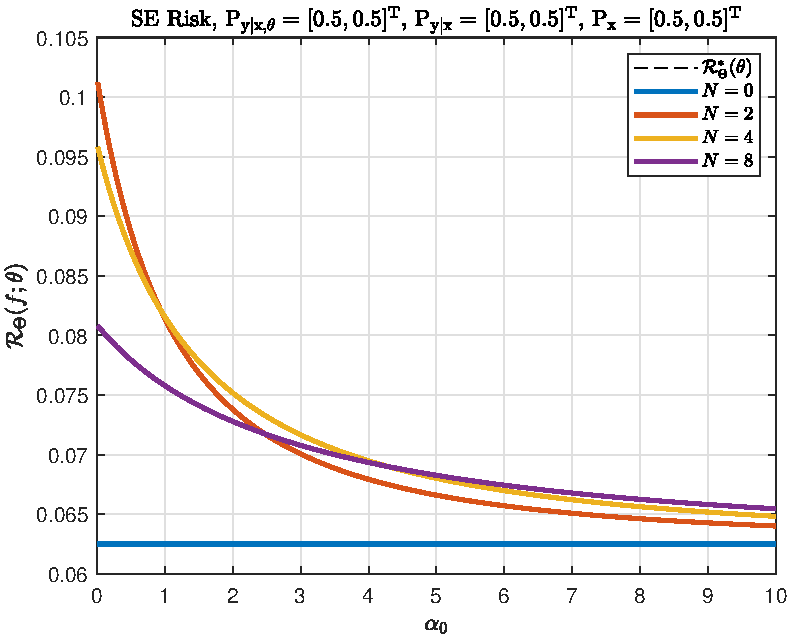
\includegraphics[width=0.7\linewidth]{Risk_cond_SE_Dir_a0_leg_N_unbiased.pdf}
	\caption{Conditional SE Risk versus $\alpha_0 \alpham(x)$, unbiased Dirichlet estimator using varying training set volumes}
	\label{fig:Risk_cond_SE_Dir_a0_leg_N_unbiased}
\end{figure}
\begin{figure}
	\centering
	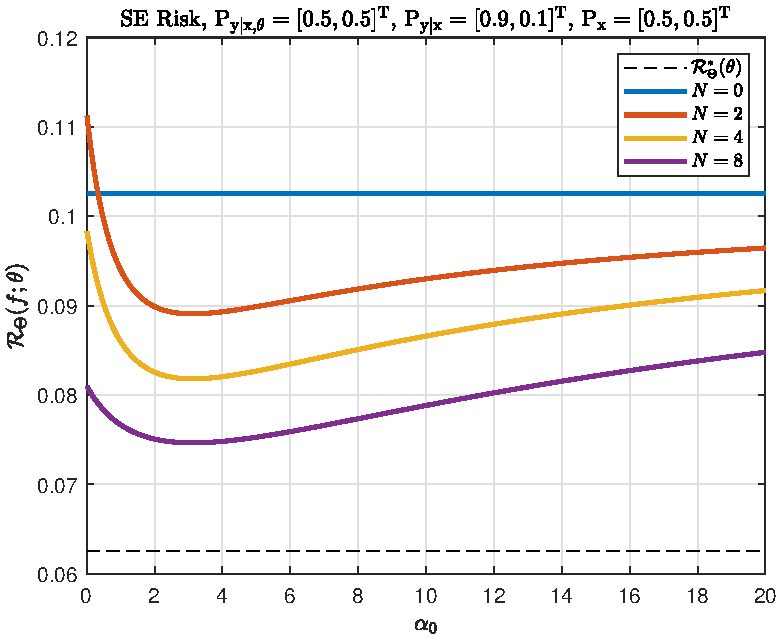
\includegraphics[width=0.7\linewidth]{Risk_cond_SE_Dir_a0_leg_N_biased.pdf}
	\caption{Conditional SE Risk versus $\alpha_0$, biased Dirichlet estimator using varying training set volumes}
	\label{fig:Risk_cond_SE_Dir_a0_leg_N_biased}
\end{figure}

PGR: plot captions, alpha zero or x???

















\newpage

\appendix



\chapter{Discrete-Domain Random Processes}

\todolo{LOTS of redundancy...}

This chapter details the properties of various discrete-domain random processes. The domain $\Ycal$ is assumed countable.


\section{Empirical Distribution Properties}
\label{app:emp}

\subsection{Aggregation}

\todomid{integer z? remove? use i?}

\todomid{concatenation notation?}

A characteristic of an Empirical random process is that its aggregations are also Empirical processes. Consider a random process $\uppsi \sim \Emp(N,\theta)$ drawn from $\Uppsi \subset \Pcal(\Ycal)$ for $N$ samples and mean function $\theta$. Define an arbitrary partition of $\Ycal$: $\left\{ \ldots,\Scal_z,\ldots \right\}$, $z \in \Zcal$ and the corresponding function partitions $\uppsi_z \in \Rbbgeq^{\Scal_z}$, such that $\uppsi = \left( \ldots,\uppsi_z,\ldots \right)$, and $\theta_z \in \Rbbgeq^{\Scal_z}$, such that $\theta = \left( \ldots,\theta_z,\ldots \right)$. The transformed random process $\uppsim \in \Uppsim \subset \Pcal(\Zcal)$, defined as $\uppsim(z) \equiv \sum_{y \in \Scal_z} \uppsi_z(y)$, is distributed as $\uppsim \sim \Emp(N,\thetam)$ with a parameterizing distribution $\upthetam$ defined as $\thetam(z) = \sum_{y \in \Scal_z} \theta_z(y)$.

To prove this principle, define the subset 
\begin{IEEEeqnarray}{rCl}
\Uppsi'(\psim) & = & \prod_{z \in \Zcal} \Uppsi'_z\big( \psim(z) \big) \nonumber \\
& = & \prod_{z \in \Zcal} \left\{ n_z / N : n_z \in \Zbbgeq^{\Scal_z}, \ \sum_{y \in \Scal_z} n_z(y) = N \psim(z) \right\} \subset \Uppsi
\end{IEEEeqnarray}
and observe that
\begin{IEEEeqnarray}{rCl}
\Prm_{\uppsim | \uptheta}(\psim | \theta) & = & \sum_{\psi \in \Uppsi'(\psim)} \Prm_{\uppsi | \uptheta}(\psi | \theta) 
= \sum_{\psi \in \Uppsi'(\psim)} \Mcal(N \psi) \left( \prod_{y \in \Ycal} \theta(y)^{\psi(y)} \right)^N \\
& = & \Mcal(N \psim) \prod_{z \in \Zcal} \sum_{\psi_z \in \Uppsi'_z\big( \psim(z) \big)} \Mcal( N \psi_z ) \left( \prod_{y \in \Scal_z} \theta_z(y)^{\psi_z(y)} \right)^N \nonumber \\
& \equiv & \Mcal(N \psim) \left( \prod_{z \in \Zcal} \thetam(z)^{\psim(z)} \right)^N = \Emp(\psim ; N,\thetam) \nonumber \;,
\end{IEEEeqnarray}
where the multinomial theorem \cite{graham} has been used.




\subsection{Conditioned on its Aggregation}

If the Empirical random process $\uppsi$ is conditioned on its aggregation $\uppsim$ over the partition $\left\{ \ldots,\Scal_z,\ldots \right\}$, $z \in \Zcal$, the distinct segments $\uppsi_z$ become independent random processes, such that for $\psi \in \Uppsi'(\psim)$,
\begin{IEEEeqnarray}{rCl}
\Prm_{\uppsi | \uppsim,\uptheta}(\psi | \psim,\theta) & = & \frac{\Prm_{\uppsi,\uppsim | \uptheta}(\psi,\psim | \theta)}{\Prm_{\uppsim | \uptheta}(\psim | \theta)} \equiv \frac{\Mcal(N \psi)}{\Mcal(N \psim)} \left( \frac{\prod_{y \in \Ycal} \theta(y)^{\psi(y)}}{\prod_{z \in \Zcal} \thetam(z)^{\psim(z)}} \right)^N \\
& = & \prod_{z \in \Zcal} \Bigg[ \Mcal(N \psi_z) \left(\frac{\prod_{y \in \Scal_z} \theta_z(y)^{\psi_z(y)}}{\thetam(z)^{\psim(z)}} \right)^N \Bigg] \nonumber \\
& = & \prod_{z \in \Zcal} \Bigg[ \Mcal(N \psi_z) \left( \prod_{y \in \Scal_z} \left(\frac{\theta_z(y)}{\thetam(z)}\right)^{\psi_z(y)} \right)^N \Bigg] \nonumber \;.
\end{IEEEeqnarray}

While these function segments are independent, they are not Empirical processes. Introducing the conditional distributions $\thetac(z) \equiv \theta_z / \thetam(z)$ and the normalized segments $\uppsic(z) \equiv \uppsi_z / \uppsim(z) \in \Pcal(\Scal_z)$, it can be shown that
\begin{IEEEeqnarray}{rCl}
\Prm_{\uppsic | \uppsim,\uptheta}(\psic | \psim,\theta) & \equiv & \prod_{z \in \Zcal} \Bigg[ \Mcal\big( N \psim(z) \psic(z) \big) \left( \prod_{y \in \Scal_z} \thetac(y;z)^{\psic(y;z)} \right)^{N \psim(z)} \Bigg] \nonumber \\
& = & \prod_{z \in \Zcal} \Emp\Big( \psic(z) ; N \psim(z), \thetac(z) \Big) \;.
\end{IEEEeqnarray}
Thus, when also conditioned on the aggregation $\uppsim$, the individual random processes $\uppsic(z)$ are independent Empirical processes of $N \uppsim(z)$ samples, parameterized by the distributions $\thetac(z) \in \Pcal(\Scal_z)$.









%\section{Multinomial Distribution Properties}
%\label{app:multi}
%
%\todohi{Even needed in addition to EMP proofs? Replace psi?}
%
%\subsection{Aggregation}
%
%\todomid{Redundant given citation??}
%
%A characteristic of a Multinomial random process is that its aggregations are also Multinomial. Consider a random process $\uppsi \sim \Multi(N,\theta) \in \Uppsi$ over the countable set $\Ycal$. Define an arbitrary partition of $\Ycal$: $\left\{ \ldots,\Scal_z,\ldots \right\}$, $z \in \Zcal$ and the corresponding function partitions $\uppsi_z \in \Rbbgeq^{\Scal_z}$, such that $\uppsi = \left\{ \ldots,\uppsi_z,\ldots \right\}$ and $\theta_z \in \Rbbgeq^{\Scal_z}$, such that $\theta = \left\{ \ldots,\theta_z,\ldots \right\}$. The transformed random process $\uppsim(z) \equiv \sum_{y \in \Scal_z} \uppsi_z(y)$ is distributed as $\uppsim \sim \Multi(N,\thetam)$ with a parameterizing distribution defined as $\thetam(z) = \sum_{y \in \Scal_z} \theta_z(y)$.
%
%To prove this principle, define the subset 
%\begin{IEEEeqnarray}{rCl}
%\Uppsi'(\psim) & = & \prod_{z \in \Zcal} \Uppsi'_z\big( \psim(z) \big) \nonumber \\
%& = & \prod_{z \in \Zcal} \left\{ n_z / N : n_z \in \Zbbgeq^{\Scal_z}, \ \sum_{y \in \Scal_z} n_z(y) = N \psim(z) \right\} \subset \Uppsi
%\end{IEEEeqnarray}
%%\begin{IEEEeqnarray}{rCl}
%%\Uppsim(\psim) & = & \big\{ \psi \in \Uppsi : \sum_{y \in \Scal_z} \psi_z(y) = \psim(z), \ \forall z \in \Zcal \big\} \nonumber \\
%%& = & \left\{ n / N : n \in \Zbbgeq^{\Ycal}, \ \sum_{y \in \Scal_z} n(y) = N \psim(z), \ \forall z \in \Zcal \right\} \subseteq \Uppsi
%%\end{IEEEeqnarray}
%Next, observe that
%\begin{IEEEeqnarray}{rCl}
%\Prm_{\uppsim}(\psim) & = & \sum_{\psi \in \Uppsi'(\psim)} \Prm_{\uppsi}(\psi) 
%= \sum_{\psi \in \Uppsi'(\psim)} \Mcal(\psi) \prod_{y \in \Ycal} \theta(y)^{\psi(y)} \\
%& = & \Mcal(\psim) \prod_{z \in \Zcal} \sum_{\psi_z \in \Uppsi'_z(\psim)} \Mcal( \psi_z ) \prod_{y \in \Scal_z} \theta_z(y)^{\psi_z(y)} \nonumber \\
%& = & \Mcal(\psim) \prod_{z \in \Zcal} \thetam(z)^{\psim(z)} = \Multi(\psim ; N,\thetam) \nonumber \;,
%\end{IEEEeqnarray}
%where the multinomial theorem \cite{graham} has been used.
%
%
%
%\subsection{Conditioned on its Aggregation}
%
%If the multinomial random process $\uppsi$ is conditioned on its aggregation $\uppsim$ over the partition $\left\{ \ldots,\Scal_z,\ldots \right\}$, $z \in \Zcal$, the distinct segements $\uppsi_z$ become independent random processes, such that for $\psi \in \Uppsi'(\psim)$,
%
%If the multinomial random process $\uppsi$ is conditioned on its aggregation over the partition $\left\{ \ldots,\Scal_z,\ldots \right\}$, $z \in \Zcal$, the distinct segements $\uppsi_z$ become independent multinomial random processes
%\begin{IEEEeqnarray}{rCl}
%\Prm_{\uppsi | \uppsim}(\psi | \psim) & = & \frac{\Mcal(\psi) \prod_{y \in \Ycal} \theta(y)^{\psi(y)}}{\Mcal(\psim) \prod_{z \in \Zcal} \thetam(z)^{\psim(z)}} \\
%& = & \prod_{z \in \Zcal} \Bigg[ \Mcal(\psi_z) \prod_{y \in \Scal_z} \left(\frac{\theta_z(y)}{\thetam(z)}\right)^{\psi_z(y)} \Bigg] \nonumber \\
%& = & \prod_{z \in \Zcal} \Bigg[ \Mcal(\psi_z) \prod_{y \in \Scal_z} \thetac(y;z)^{\psi_z(y)} \Bigg] \nonumber \\
%& = & \prod_{z \in \Zcal} \Multi\big( \psi_z ; \psim(z) , \thetac(z) \big) \nonumber \;,
%\end{IEEEeqnarray}
%parameterized by the conditional distributions $\thetac(z) \equiv \theta_z / \thetam(z) \in \Pcal(\Scal_z)$.









\section{Dirichlet Distribution Properties}
\label{app:Dir_agg}


\subsection{Aggregation}

It is known that Dirichlet aggregations are also Dirichlet \cite{ferguson}. Let the random process $\uptheta \sim \Dir(\alpha_0,\alpha)$ drawn from $\Uptheta \equiv \Pcal(\Ycal)$ be Dirichlet with concentration $\alpha_0 \in \Rbb^+$ and mean function $\alpha \in \left\{ {\Rbb^+}^{\Ycal} : \sum_{y \in \Ycal} \alpha(y) = 1 \right\}$. Define an arbitrary partition of $\Ycal$: $\left\{ \ldots,\Scal_z,\ldots \right\}$, $z \in \Zcal$ and the corresponding function partitions $\uptheta_z \in \Rbbgeq^{\Scal_z}$, such that $\uptheta = \left( \ldots,\uptheta_z,\ldots \right)$ and $\alpha_z \in {\Rbb^+}^{\Scal_z}$, such that $\alpha = \left( \ldots,\alpha_z,\ldots \right)$. The transformed random process $\upthetam \in \Pcal(\Zcal)$, defined as $\upthetam(z) \equiv \sum_{y \in \Scal_z} \uptheta_z(y)$, is distributed as $\upthetam \sim \Dir(\alpha_0,\alpham)$ with a parameterizing distribution $\alpham$ defined as $\alpham(z) = \sum_{y \in \Scal_z} \alpha_z(y)$.

To prove this principle, define the subset 
\begin{IEEEeqnarray}{rCl}
\Uptheta'(\thetam) & = & \prod_{z \in \Zcal} \Uptheta'_z\big( \thetam(z) \big) \nonumber \\
& = & \prod_{z \in \Zcal} \left\{ \theta_z \in \Rbbgeq^{\Scal_z} : \ \sum_{y \in \Scal_z} \theta_z(y) = \thetam(z) \right\} \subset \Uptheta
\end{IEEEeqnarray}
and note that
\begin{IEEEeqnarray}{rCl}
\prm_{\upthetam}(\thetam) & = & \int_{\Uptheta'(\thetam)} \prm_{\uptheta}(\theta) {\drm}\theta = \int_{\Uptheta'(\thetam)} \beta(\alpha_0 \alpha)^{-1} \prod_{y \in \Ycal} \theta(y)^{\alpha_0 \alpha(y) - 1} {\drm}\theta \nonumber \\
& = & \beta(\alpha_0 \alpha)^{-1} \prod_{z \in \Zcal} \int_{\Uptheta'_z\big( \thetam(z) \big)} \prod_{y \in \Scal_z} \theta_z(y)^{\alpha_0 \alpha_z(y)-1} {\drm}\theta_z \nonumber \\
& = & \beta(\alpha_0 \alpha)^{-1} \prod_{z \in \Zcal} \thetam(z)^{\alpha_0 \alpham(z) - 1} \int_{{\Uptheta''}_z} \prod_{y \in \Scal_z} \thetac(y;z)^{\alpha_0 \alpha_z(y)-1} {\drm}\thetac(z) \nonumber \\
& = & \beta(\alpha_0 \alpha)^{-1} \prod_{z \in \Zcal} \thetam(z)^{\alpha_0 \alpham(z) - 1} \beta(\alpha_0 \alpha_z) \nonumber \\
& = & \beta(\alpha_0 \alpha_m)^{-1} \prod_{z \in \Zcal} \thetam(z)^{\alpha_0 \alpham(z) - 1} = \Dir(\thetam; \alpha_0,\alpham)
\end{IEEEeqnarray}
where the transform $\thetac(z) \equiv \theta_z / \thetam(z) \in {\Uptheta''}_z = \left\{ \theta_z \in \Rbbgeq^{\Scal_z} : \ \sum_{y \in \Scal_z} \theta_z(y) = 1 \right\}$ has been used. Note that the determinant of the transform dictates ${\drm}\thetac(z) = \thetam(z)^{1-|\Scal_z|} {\drm}\theta_z$.

\todolo{cite Jacobian?}



\subsection{Conditioned on its Aggregation}

This section details another important property of Dirichlet distributed random processes: when conditioned on its own aggregation $\upthetam$, the partitioned segments $\uptheta_z$ of the process become independent. Furthermore, the normalized functions $\upthetac(z)$ are also Dirichlet processes. 

The PDF of the original random process $\uptheta$ conditioned on its aggregation $\upthetam$ can be formulated as
\begin{IEEEeqnarray}{rCl}
\prm_{\uptheta | \upthetam}(\theta | \thetam) & = & \frac{\beta(\alpha_0 \alpha_m) \prod_{y \in \Ycal} \theta(y)^{\alpha_0 \alpha(y)-1}}{\beta(\alpha_0 \alpha) \prod_{z \in \Zcal} \thetam(z)^{\alpha_0 \alpham(z)-1}} \\
& \equiv & \prod_{z \in \Zcal} \Bigg[ \beta( \alpha_0 \alpha_z )^{-1} \frac{\prod_{y \in \Scal_z} \theta_z(y)^{\alpha_0 \alpha_z(y)-1}}{\thetam(z)^{\alpha_0 \alpham(z)-1}} \Bigg] \nonumber \\ 
& = & \prod_{z \in \Zcal} \Bigg[ \frac{\thetam(z)^{1-|\Scal_z|}}{\beta( \alpha_0 \alpha_z )} \prod_{y \in \Scal_z} \left(\frac{\theta_z(y)}{\thetam(z)}\right)^{\alpha_0 \alpha_z(y)-1} \Bigg] \nonumber \;,
\end{IEEEeqnarray}
which is defined for $\prod_{z \in \Zcal} \left\{ \theta_z \in {\Rbbgeq}^{\Scal_z} : \sum_{y \in \Scal_z} \theta_z(y) = \thetam(z) \right\}$.
%$\left\{ \theta \in {\Rbbgeq}^{\Ycal} : \sum_{y \in \Scal_z} \theta(y) = \thetam(z), \ \forall z \in \Zcal \right\}$

Observe that the partitioned segements $\uptheta_z$ are conditionally independent. Introducing the normalized functions $\alphac(z) \equiv \alpha_z / \alpham(z)$ and the normalized random processes $\upthetac(z) \equiv \uptheta_z / \upthetam(z) \in \Pcal(\Scal_z)$, it can be shown that
\begin{IEEEeqnarray}{rCl}
\prm_{\upthetac | \upthetam}\left( \thetac | \thetam \right) & = & \prod_{z \in \Zcal} \Bigg[ \beta\big( \alpha_0 \alpham(z) \alphac(z) \big)^{-1} \prod_{y \in \Scal_z} \thetac(y;z)^{\alpha_0 \alpham(z) \alphac(y;z)-1} \Bigg] \\
& = & \prod_{z \in \Zcal} \Dir\big( \thetac(z) ; \alpha_0 \alpha_m(z), \alphac(z) \big) \nonumber \;.
\end{IEEEeqnarray}
Thus after conditioning, the normalized processes $\upthetac(z)$ are Dirichlet distributed, independent of one another, and independent of the aggregation $\upthetam$. 

PGR: discuss transform Jacobian and dimensionality? 










\section{Dirichlet-Empirical Distribution Properties} 
\label{app:DE}

\subsection{Aggregation}

The Dirichlet-Empirical distribution is so named since it is the expectation of a Empirical distribution $\Emp(N,\uptheta)$ with respect to its mean function, a Dirichlet process $\uptheta \sim \Dir(\alpha_0, \alpha)$. Naturally, these random processes share many properties with the Empirical distribution.

A characteristic of a Dirichlet-Empirical random process is that its aggregations are also Dirichlet-Empirical - this is inherited from the related Dirichlet-Multinomial distribution \cite{johnson}. Consider a DE random process $\uppsi \sim \DE(N,\alpha_0,\alpha)$ drawn from $\Uppsi \subset \Pcal(\Ycal)$ of $N$ samples, concentration $\alpha_0$ and mean function $\alpha$. Define an arbitrary partition of $\Ycal$: $\left\{ \ldots,\Scal_z,\ldots \right\}$, $z \in \Zcal$ and the corresponding function partitions $\uppsi_z \in \Rbbgeq^{\Scal_z}$, such that $\uppsi = \left( \ldots,\uppsi_z,\ldots \right)$, and $\alpha_z \in {\Rbb^+}^{\Scal_z}$, such that $\alpha = \left( \ldots,\alpha_z,\ldots \right)$. The transformed random process $\uppsim \in \Uppsim \subset \Pcal(\Zcal)$, defined as $\uppsim(z) \equiv \sum_{y \in \Scal_z} \uppsi_z(y)$, is distributed as $\uppsim \sim \DE(N,\alpha_0,\alpham)$ with mean function $\alpham$ defined as $\alpham(z) = \sum_{y \in \Scal_z} \alpha_z(y)$.

To prove this principle, define the subset 
\begin{IEEEeqnarray}{rCl}
\Uppsi'(\psim) & = & \prod_{z \in \Zcal} \Uppsi'_z\big( \psim(z) \big) \nonumber \\
& = & \prod_{z \in \Zcal} \left\{ n_z / N : n_z \in \Zbbgeq^{\Scal_z}, \ \sum_{y \in \Scal_z} n_z(y) = N \psim(z) \right\} \subset \Uppsi
\end{IEEEeqnarray}
%\begin{IEEEeqnarray}{rCl}
%\Uppsim(\psim) & = & \big\{ \psi \in \Uppsi : \sum_{y \in \Scal_z} \psi_z(y) = \psim(z), \ \forall z \in \Zcal \big\} \nonumber \\
%& = & \left\{ n / N : n \in \Zbbgeq^{\Ycal}, \ \sum_{y \in \Scal_z} n(y) = N \psim(z), \ \forall z \in \Zcal \right\} \subseteq \Uppsi
%\end{IEEEeqnarray}
Next, observe that
\begin{IEEEeqnarray}{rCl}
\Prm_{\uppsim}(\psim) & = & \sum_{\psi \in \Uppsi'(\psim)} \Prm_{\uppsi}(\psi) 
= \sum_{\psi \in \Uppsi'(\psim)} \Mcal(N \psi) \frac{\beta(\alpha_0 \alpha + N \psi)}{\beta(\alpha_0 \alpha)} \\
& = & \Mcal(N \psim) \frac{\beta(\alpha_0 \alpham + N \psim)}{\beta(\alpha_0 \alpha)} \prod_{z \in \Zcal} \sum_{\psi_z \in \Uppsi'_z\big(\psim(z)\big)} \Mcal( N \psi_z ) \frac{\beta(\alpha_0 \alpha_z + N \psi_z)}{\beta(\alpha_0 \alpha_z)} \nonumber \\
& = & \Mcal(N \psim) \frac{\beta(\alpha_0 \alpham + N \psim)}{\beta(\alpha_0 \alpha)} = \DE(\psim ; N,\alpha_0,\alpham) \nonumber \;,
\end{IEEEeqnarray}
where the identity
\begin{equation}
\sum_{\substack{n \in \Zbbgeq^{\Ycal}: \\ \sum_y n(y) = N}} \Mcal(n) \beta(a + n) = \beta\left( a \right)
\end{equation}
has been used.

\todolo{more proof steps?}

\todolo{cite identity}


\subsection{Conditioned on its Aggregation}

If the Dirichlet-Empirical random process $\uppsi$ is conditioned on its aggregation $\uppsim$ over the partition $\left\{ \ldots,\Scal_z,\ldots \right\}$, $z \in \Zcal$, the distinct segements $\uppsi_z$ become independent random processes, such that for $\psi \in \Uppsi'(\psim)$,
\begin{IEEEeqnarray}{rCl}
\Prm_{\uppsi | \uppsim}(\psi | \psim) & = & \frac{\Mcal(N \psi) \beta(\alpha_0 \alpha)^{-1} \beta(\alpha_0 \alpha + N \psi)}{\Mcal(N \psim) \beta(\alpha_0 \alpham)^{-1} \beta(\alpha_0 \alpham + N \psim)} \\
& = & \left( \prod_{z \in \Zcal} \frac{\Gamma\big( \alpha_0 \alpham(z)+N \psim(z) \big)}{\big(N \psim(z)\big)! \ \Gamma\big( \alpham(z) \big)} \right)^{-1} \left( \prod_{y \in \Ycal} \frac{\Gamma\big( \alpha_0 \alpha(y) + N \psi(y) \big)}{\big(N \psi(y)\big)! \ \Gamma\big( \alpha_0 \alpha(y) \big)} \right) \nonumber \\
& = & \prod_{z \in \Zcal} \left[ \frac{\big(N \psim(z)\big)! \ \Gamma\big( \alpham(z) \big)}{\Gamma\big( \alpha_0 \alpham(z)+N \psim(z) \big)} \prod_{y \in \Scal_z} \frac{\Gamma\big( \alpha_0 \alpha_z(y) + N \psi_z(y) \big)}{\big(N \psi_z(y)\big)! \ \Gamma\big( \alpha_0 \alpha_z(y) \big)} \right] \nonumber \\
& = & \prod_{z \in \Zcal} \Mcal(N \psi_z) \frac{\beta(\alpha_0 \alpha_z + N \psi_z)}{\beta(\alpha_0 \alpha_z)} \nonumber ;.
\end{IEEEeqnarray}

While these individual function segments are independent, they are not Dirichlet-Empirical processes. Defining the functions $\alphac(z) \equiv \alpha_z / \alpham(z) \in \Pcal(\Scal_z)$ and the normalized segments $\uppsic(z) \equiv \uppsi_z / \uppsim(z) \in \Pcal(\Scal_z)$, it can be shown that
\begin{IEEEeqnarray}{rCl}
\Prm_{\uppsic | \uppsim}(\psic | \psim) & = & \prod_{z \in \Zcal} \Mcal\big( N \psim(z) \psic(z) \big) \frac{\beta\big( \alpha_0 \alpham(z) \alphac(z) + N \psim(z) \psic(z) \big)}{\beta\big( \alpha_0 \alpham(z) \alphac(z) \big)} \nonumber \\
& = & \prod_{z \in \Zcal} \DE\Big( \psic(z) ; N \psim(z), \alpha_0 \alpham(z), \alphac(z) \Big) \;,
\end{IEEEeqnarray}
Thus, when conditioned on the aggregation $\uppsim$, the individual functions $\uppsic(z) \in \Pcal(\Scal_z)$ are independent Dirichlet-Empirical processes of $N \uppsim(z)$ samples and concentration $\alpha_0 \alpham(z)$, with mean functions $\alphac(z)$.

\todohi{Double check.}










%\section{Dirichlet-Multinomial Process conditioned on its aggregation} 
%\label{app:DM_agg}
%
%\todohi{Even needed in addition to DE proofs? Replace psi? INCOMPLETE}
%
%
%A defining characteristic of a Dirichlet-Multinomial random process is that its aggregations are also Dirichlet-Multinomial \cite{johnson}. Consider a DM random process $\uppsi \sim \DM(N,\alpha)$ over the countable set $\Ycal$. Define an arbitrary partition of $\Ycal$: $\left\{ \ldots,\Scal_z,\ldots \right\}$, $z \in \Zcal$; the transformed random process $\uppsim(z) \equiv \sum_{y \in \Scal_z} \uppsi(y)$ is neccessarily Dirichlet-Multinomial with parameterizing function $\alpham(z) = \sum_{y \in \Scal_z} \alpha(y)$.
%
%It can be shown that conditioned on the aggregation $\uppsim$, the segments $\big\{ \uppsi(y) : y \in \Scal_z \big\}$ of the original random process become independent Dirichlet-Multinomial random processes, such that
%\begin{IEEEeqnarray}{rCl}
%\Prm_{\uppsic | \uppsim}(\psic | \psim) & = & \frac{\Mcal(N \psi) \beta(\alpha_0 \alpha)^{-1} \beta(\alpha_0 \alpha + N \psi)}{\Mcal(N \psim) \beta(\alpha_0 \alpham)^{-1} \beta(\alpha_0 \alpham + N \psim)} \\
%& = & \left( \prod_{z \in \Zcal} \frac{\Gamma\big( \alpha_0 \alpham(z)+N \psim(z) \big)}{\big(N \psim(z)\big)! \ \Gamma\big( \alpham(z) \big)} \right)^{-1} \left( \prod_{y \in \Ycal} \frac{\Gamma\big( \alpha_0 \alpha(y) + N \psi(y) \big)}{\big(N \psi(y)\big)! \ \Gamma\big( \alpha_0 \alpha(y) \big)} \right) \nonumber \\
%& = & \prod_{z \in \Zcal} \left[ \frac{\big(N \psim(z)\big)! \ \Gamma\big( \alpham(z) \big)}{\Gamma\big( \alpha_0 \alpham(z)+N \psim(z) \big)} \prod_{y \in \Scal_z} \frac{\Gamma\big( \alpha_0 \alpha(y) + N \psi(y) \big)}{\big(N \psi(y)\big)! \ \Gamma\big( \alpha_0 \alpha(y) \big)} \right] \nonumber \\
%& = & \prod_{z \in \Zcal} \DM\Big( \big\{ \psi(y) : y \in \Scal_z \big\} ; \psim(z), \big\{ \alpha(y) : y \in \Scal_z \big\} \Big) \nonumber \;,
%\end{IEEEeqnarray}
%%\begin{IEEEeqnarray}{rCl}
%%\Prm(\uppsi | \uppsim) & = & \frac{\Prm(\uppsi)}{\Prm(\uppsim)} \Prm(\uppsim | \uppsi) \\ 
%%& = & \frac{\Mcal(\uppsi) \beta(\alpha_0 \alpha)^{-1} \beta(\alpha+\uppsi)}{\Mcal(\uppsim) \beta(\alpha_0 \alpham)^{-1} \beta(\alpha'+\uppsim)} \prod_{z \in \Zcal} \delta\left[ \uppsim(z),\sum_{y \in \Scal_z} \uppsi(y) \right] \nonumber \\
%%& = & \left( \prod_{z \in \Zcal} \frac{\Gamma\big( \alpham(z)+\uppsim(z) \big)}{\uppsim(z)! \ \Gamma\big( \alpham(z) \big)} \right)^{-1} \left( \prod_{y \in \Ycal} \frac{\Gamma\big( \alpha(y)+\uppsi(y) \big)}{\uppsi(y)! \ \Gamma\big( \alpha_0 \alpha(y) \big)} \right) \nonumber \\
%%&& \quad \prod_{z \in \Zcal} \delta\left[ \uppsim(z),\sum_{y \in \Scal_z} \uppsi(y) \right] \nonumber \\
%%& = & \prod_{z \in \Zcal} \left[ \delta\left[ \uppsim(z),\sum_{y \in \Scal_z} \uppsi(y) \right] \frac{\uppsim(z)! \ \Gamma\big( \alpham(z) \big)}{\Gamma\big( \alpham(z)+\uppsim(z) \big)} \prod_{y \in \Scal_z} \frac{\Gamma\big( \alpha(y)+\uppsi(y) \big)}{\uppsi(y)! \ \Gamma\big( \alpha_0 \alpha(y) \big)} \right] \nonumber \\
%%& = & \prod_{z \in \Zcal} \DM\Big( \big\{ \uppsi(y) : y \in \Scal_z \big\} ; \uppsim(z), \big\{ \alpha(y) : y \in \Scal_z \big\} \Big) \nonumber \;,
%%\end{IEEEeqnarray}
%on the domain $\left\{ \psi \in {\Zbbgeq}^{\Ycal} : \sum_{y \in \Scal_z} \psi(y) = \psim(z), \quad \forall z \in \Zcal \right\}$. 







\chapter{Continuous-Domain Random Processes}

This chapter details the properties of various continuous-domain random processes. The domain $\Ycal$ is assumed to be a continuous set.


\section{Empirical Process Properties} \label{app:EP}


\subsection{Definition}

This section introduces a new continuous-domain random process, referred to as the Empirical process (EP). It is the generalization of the Empirical distribution for i.i.d. samples drawn from a continuous set. The Empirical process $\uppsi \sim \EP(N,\theta)$ is parameterized by $N$ samples and mean function $\theta \in \Pcal(\Ycal)$; it assumes functions from the set $\Uppsi = \left\{ N^{-1} \sum_{n=1}^N \delta(\cdot - D_n) : D \in \Ycal^N \right\} \subset \Pcal(\Ycal)$.

The continuous-domain Empirical process is characterized by the same aggregation property as its discrete-domain variant. Define a countable partition of $\Ycal$, $\left\{ \ldots,\Scal_z,\ldots \right\}$, $z \in \Zcal$, and the corresponding function partitions $\uppsi_z \in \Rbbgeq^{\Scal_z}$, such that $\uppsi = \left( \ldots,\uppsi_z,\ldots \right)$, and $\theta_z \in \Rbbgeq^{\Scal_z}$, such that $\theta = \left( \ldots,\theta_z,\ldots \right)$. Thus, for an Empirical process $\uppsi \in \Uppsi$, the aggregation $\uppsim \in \Uppsim \subset \Pcal(\Xcal)$ satisfying $\uppsim(z) \equiv \int_{\Scal_z} \uppsi_z(y) {\drm}y$ is an Empirical process with $N$ samples and mean function $\thetam$ satisfying $\thetam(z) \equiv \int_{\Scal_z} \theta_z(y) {\drm}y$.

Additionally, when further conditioned on the aggregation $\uppsim$, the normalized random processes $\uppsic(z) \equiv \uppsi_z / \uppsim(z)$ are independent continuous-domain Empirical processes, $\uppsic(z) | \uppsim(z), \upthetac(z) \sim \EP\big(N \uppsim(z), \upthetac(z)\big)$, where $\thetac(z) \equiv \theta_z / \thetam(z) \in \Pcal(\Scal_z)$.







%\subsection{Mean and Correlation Functions}
%
%In this subsection the mean and correlation functions of a continuous-domain EP are expressed. The mean function is
%\begin{IEEEeqnarray}{rCl}
%\mu_{\uppsi | \uptheta} & = & \Erm_{\Drm | \uptheta}\left[ \frac{1}{N} \sum_{n=1}^N \delta\big( \cdot - \Drm_n \big) \right] \\
%& = & \frac{1}{N} \sum_{n=1}^N \Prm_{\Drm_n | \uptheta} = \frac{1}{N} \sum_{n=1}^N \uptheta \nonumber \\
%& = & \uptheta \nonumber \;.
%\end{IEEEeqnarray}
%
%\todolo{Binomial RV proof? Like DP?}
%
%The correlation function is
%\begin{IEEEeqnarray}{rCl}
%\Erm_{\uppsi | \uptheta}\big[ \uppsi(y) \uppsi(y') \big] & = & N^{-2} \sum_{n=1}^N \sum_{n'=1}^N \Erm_{\Drm | \uptheta}\Big[ \delta\big( y-\Drm_n \big) \delta\big( y'-\Drm_{n'} \big) \Big] \nonumber \\
%& = & N^{-2} \sum_n \Erm_{\Drm_n | \uptheta}\Big[ \delta\big( y-\Drm_n \big) \delta\big( y'-\Drm_n \big) \Big] \nonumber \\
%&& \quad + N^{-2} \sum_{n \neq n'} \Erm_{\Drm_n | \uptheta}\Big[ \delta\big( y-\Drm_n \big) \Big] \Erm_{\Drm_{n'} | \uptheta}\Big[ \delta\big( y'-\Drm_{n'} \big) \Big] \nonumber \\
%& = & N^{-2} \sum_n \int_{\Ycal} \uptheta(\tilde{y}) \delta(y-\tilde{y}) \delta(y'-\tilde{y}) {\drm}\tilde{y}  \nonumber \\
%&& \quad + N^{-2} \sum_{n \neq n'} \int_{\Ycal} \uptheta(\tilde{y}) \delta(y-\tilde{y}) {\drm}\tilde{y} \int_{\Ycal} \uptheta(\tilde{y}') \delta(y'-\tilde{y}') {\drm}\tilde{y}' \nonumber \\
%& = & \frac{1}{N} \uptheta(y) \delta(y-y') + \left(1-\frac{1}{N}\right) \uptheta(y) \uptheta(y') \;.
%\end{IEEEeqnarray}


\subsection{Mean and Correlation Functions} \label{app:E_EP}

In this section, it is shown that the expected value of an Empirical process $\uppsi \sim \EP(N, \theta)$ is 
\begin{equation}
\mu_{\uppsi} = \theta \;.
\end{equation}

A defining characteristic of Empirical processes is that their aggregations are also Empirical. Define the partition of $\Ycal = \Rbb$, $\big\{ \Scal(y),S^\text{c}(y) \big\}$ where $\Scal(y) = (-\infty,y]$. The transform random process $\big(\uppsim, \uppsim^\text{c}\big)$, where $\uppsim \equiv \int_{\infty}^y \uppsi(t) {\drm}t$, is thus a discrete-domain Empirical random process for $N$ samples and mean $\big(\thetam,\thetam^\text{c}\big)$, where $\thetam = \int_{-\infty}^y \theta(t) {\drm}t$ and $\thetam^\text{c} = \int_y^\infty \theta(t) {\drm}t$. Dependency on $y$ is suppressed for brevity. Observe that $\mu_{\uppsim}(y) = \thetam$ and thus that 
\begin{IEEEeqnarray}{rCl}
\mu_{\uppsim} & = & \int_{-\infty}^y \theta(t) {\drm}t = \int_{-\infty}^y \mu_{\uppsi}(t) {\drm}t \nonumber \;.
\end{IEEEeqnarray}
Differentiating with respect to $y$, we have the expected value of the EP.

Next, the correlation function is shown to be 
\begin{equation}
\Erm_{\uppsi}\big[ \uppsi(y_1)\uppsi(y_2) \big] = \frac{1}{N} \uptheta(y_1) \delta(y_1-y_2) + \left(1-\frac{1}{N}\right) \uptheta(y_1) \uptheta(y_2) \;.
\end{equation}
First, assume $y_2 \geq y_1$ and define a new partition of $\Ycal$, $\big\{ (-\infty,y_1], (y_1,y_2], (y_2,\infty) \big\}$. By the aggregation property, the random triplet $\left( \int_{-\infty}^{y_1} \uppsi(t) {\drm}t, \int_{y_1}^{y_2} \uppsi(t) {\drm}t, \int_{y_2}^{\infty} \uppsi(t) {\drm}t \right)$ is Empirical with $N$ samples and mean $\left( \int_{-\infty}^{y_1} \theta(t) {\drm}t, \int_{y_1}^{y_2} \theta(t) {\drm}t, \int_{y_2}^{\infty} \theta(t) {\drm}t \right)$.

Define the function
\begin{IEEEeqnarray}{L}
g(t_1,t_2) = \Erm_{\uppsi}\left[ \int_{-\infty}^{y_1} \uppsi(t_1) {\drm}t_1 \int_{-\infty}^{y_2} \uppsi(t_2) {\drm}t_2 \right] \\
\quad = \Erm_{\uppsi}\left[ \left( \int_{-\infty}^{y_1} \uppsi(t_1) {\drm}t_1 \right)^2 + \left( \int_{-\infty}^{y_1} \uppsi(t_1) {\drm}t_1 \right) \left( \int_{y_1}^{y_2} \uppsi(t_2) {\drm}t_2 \right) \right] \nonumber \\
\quad = \frac{1}{N} \left( \int_{-\infty}^{y_1} \theta(t_1) {\drm}t_1 \right) \left( 1 + (N-1) \int_{-\infty}^{y_1} \theta(t_1) {\drm}t_1 \right) + \left(1-\frac{1}{N}\right) \left( \int_{-\infty}^{y_1} \theta(t_1) {\drm}t_1 \right) \left( \int_{y_1}^{y_2} \theta(t_2) {\drm}t_2 \right) \nonumber \\
\quad = \frac{1}{N} \left( \int_{-\infty}^{y_1} \theta(t_1) {\drm}t_1 \right) + \left(1-\frac{1}{N}\right) \left( \int_{-\infty}^{y_1} \theta(t_1) {\drm}t_1 \right) \left( \int_{-\infty}^{y_2} \theta(t_2) {\drm}t_2 \right) \quad \forall y_2 \geq y_1 \nonumber \;.
\end{IEEEeqnarray}
Following the same steps provides the values of $g$ for $t_2 \leq t_1$; the combined formula can be given as
\begin{IEEEeqnarray}{L}
g(t_1,t_2) = \frac{1}{N} \left( \int_{-\infty}^{\min(y_1,y_2)} \theta(t_1) {\drm}t_1 \right) + \left(1-\frac{1}{N}\right) \left( \int_{-\infty}^{y_1} \theta(t_1) {\drm}t_1 \right) \left( \int_{-\infty}^{y_2} \theta(t_2) {\drm}t_2 \right) \;. 
\end{IEEEeqnarray}
Finally,
\begin{IEEEeqnarray}{L}
\Erm_{\uppsi}\big[ \uppsi(y_1)\uppsi(y_2) \big] = \frac{{\drm}^2}{{\drm}t_1 {\drm}t_2} g(t_1,t_2) \\
\quad = \frac{{\drm}}{{\drm}t_2} \left[ \frac{1}{N} u(t_2-t_1) \theta\big( \min(t_1,t_2) \big) + \left(1-\frac{1}{N}\right) \theta(y_1) \left( \int_{-\infty}^{y_2} \theta(t_2) {\drm}t_2 \right) \right] \nonumber \\
\quad = \frac{1}{N} \theta(y_1)\delta(y_1-y_2) + \left(1-\frac{1}{N}\right) \theta(y_1)\theta(y_2) \nonumber \;.
\end{IEEEeqnarray}





\subsection{Continuous aggregation}

The aggregation property has been stated for countable partitions of the process domain - it also holds for continuous aggregations. Define an Empirical process $\uppsi \in \Uppsi$ parameterized by $N$ samples and a mean function $\theta \in \Pcal(\Ycal \times \Xcal)$. The process assumes functions from the set $\Uppsi = \left\{ N^{-1} \sum_{n=1}^N \delta(\cdot - Y_n) \delta(\cdot - X_n) : Y \in \Ycal^N, X \in \Xcal^N \right\}$. The aggregation $\uppsim \equiv \int_{\Ycal} \uppsi(y,\cdot) {\drm}y$ is an Empirical process with $N$ samples and mean function $\thetam \equiv \int_{\Ycal} \theta(y,\cdot) {\drm}y$; this characterization is inherited from the original Empirical process, as aggregations of $\uppsim$ are equivalent to aggregations of $\uppsi$. Note that $\uppsim \in \Uppsim = \left\{ N^{-1} \sum_{n=1}^N \delta(\cdot - X_n) : X \in \Xcal^N \right\}$.

Additionally, when also conditioned on the aggregation $\uppsim$, the normalized random processes $\uppsic(x) \equiv \uppsi(\cdot,x) / \uppsim(x)$ are independent continuous-domain Empirical processes, $\uppsic(x) | \uppsim(x), \upthetac(x) \sim \EP\big(\delta(0)^{-1} N \uppsim(x), \upthetac(x)\big)$, where $\thetac(x) \equiv \theta(\cdot,x) / \thetam(x) \in \Pcal(\Ycal)$.



To demonstrate this, use $\Ycal = \Xcal = \Rbb$ for simplicity. Define the countable partition of $\Ycal \times \Xcal$, $\left\{ \ldots,\Scal_i,\ldots \right\}$, $i \in \Zbb$, such that $\Scal_i = \Rbb \times \big [i\Delta,(i+1)\Delta \big)$, where $\Delta$ is an arbitrarily small interval in $\Xcal$. The corresponding function partitions are $\uppsi_i \in \Rbbgeq^{\Scal_i}$, such that $\uppsi = \left( \ldots,\uppsi_i,\ldots \right)$, and $\theta_i \in \Rbbgeq^{\Scal_i}$, such that $\theta = \left( \ldots,\theta_i,\ldots \right)$.

Introduce the aggregation process $\uppsim'(i) = \int_{\Scal_i} \uppsi_i(y,x) {\drm}y {\drm}x = \int_{i\Delta}^{(i+1)\Delta} \uppsim(x) {\drm}x$, which is Empirical with $N$ samples and mean function $\thetam'(i) = \int_{\Scal_i} \theta_i(y,x) {\drm}y {\drm}x = \int_{i\Delta}^{(i+1)\Delta} \thetam(x) {\drm}x$. By the properties of Empirical processes, the normalized functions $\uppsic'(i) \equiv \uppsi_i / \uppsim'(i)$ conditioned on $\uppsim'$ are independent Empirical processes of $N \uppsim'(i)$ samples and mean functions $\thetac'(i) \equiv \theta_i / \thetam'(i)$. Next, use the conditional aggregation to define $\uppsic''(i) = \int_{i\Delta}^{(i+1)\Delta} \uppsic'(\cdot,x;i) {\drm}x \sim \EP\big( N \uppsim'(i), \thetac''(i) \big)$, where $\thetac''(i) = \int_{i\Delta}^{(i+1)\Delta} \thetac'(\cdot,x;i) {\drm}x$. 

As $\Delta \to 0$, the conditional processes tend to $\uppsic''(i) \to \uppsic(i \Delta) \sim \EP\big( N \uppsim(i \Delta) \Delta, \uppsic(i \Delta) \big)$. Setting $x \equiv i\Delta$ and using $\delta(0) \equiv \Delta^{-1}$, the conditional model characterization given the marginal model is proven. Also, observe that $\big( \delta(0)^{-1} \uppsim(x),1 - \delta(0)^{-1} \uppsim(x)\big) \sim \Emp\Big( N, \big( \delta(0)^{-1} \thetam(x), 1 - \delta(0)^{-1} \thetam(x)\big) \Big)$ and thus that $\delta(0)^{-1} N \uppsim(x) \sim \Bi\left(N, \delta(0)^{-1} \thetam(x) \right)$.
 





\section{Dirichlet Process Properties} \label{app:DP}


\subsection{Definition}

The Dirichlet process $\uptheta \sim \Dir(\alpha_0,\alpha)$ assumes distributions from from $\Uptheta \equiv \Pcal(\Ycal)$ and is parameterized by concentration $\alpha_0 \in \Rbb^+$ and mean function $\alpha \in \left\{ {\Rbb^+}^{\Ycal} : \int_{\Ycal} \alpha(y) {\drm}y = 1 \right\}$. The continuous-domain Dirichlet process is characterized by the same aggregation property as its discrete-domain variant. Define a countable partition of $\Ycal$, $\left\{ \ldots,\Scal_z,\ldots \right\}$, $z \in \Zcal$, and the corresponding function partitions $\uptheta_z \in \Rbbgeq^{\Scal_z}$, such that $\uptheta = \left( \ldots,\uptheta_z,\ldots \right)$ and $\alpha_z \in {\Rbb^+}^{\Scal_z}$, such that $\alpha = \left( \ldots,\alpha_z,\ldots \right)$. Thus, the transformed random process $\upthetam \in \Pcal(\Zcal)$, defined as $\upthetam(z) \equiv \int_{\Scal_z} \uptheta_z(y) {\drm}y$, is Dirichlet with concentration $\alpha_0$ and mean function $\alpham$, defined as $\alpham(z) = \int_{\Scal_z} \alpha_z(y) {\drm}y$.

Additionally, the normalized random processes $\upthetac(z) \equiv \uptheta_z / \upthetam(z) \in \Pcal(\Scal_z)$ are independent continuous-domain Dirichlet processes $\upthetac(z) \sim \Dir\big(\alpha_0 \alpham(z), \alphac(z)\big)$, where $\alphac(z) \equiv \alpha_z / \alpham(z)$, and are independent of the aggregation process $\upthetam$.










\subsection{Mean and Correlation Functions} \label{app:E_DP}

In this section, it is shown that the expected value of a Dirichlet process $\uptheta \sim \DP(\alpha_0, \alpha)$ is 
\begin{equation}
\mu_{\uptheta} = \alpha \;.
\end{equation}

A defining characteristic of Dirichlet processes is that their aggregations are also Dirichlet. Define the partition of $\Ycal = \Rbb$, $\big\{ \Scal(y),S^\text{c}(y) \big\}$ where $\Scal(y) = (-\infty,y]$. The transform random variable $\upthetam \equiv \int_{-\infty}^y \uptheta(t) {\drm}t$ is thus a Beta random variable with parameters $\lambda = \alpha_0 \int_{-\infty}^y \alpha(t) {\drm}t$ and $\lambda^\text{c} = \alpha_0 \int_y^\infty \alpha(t) {\drm}t$. Dependency on $y$ is suppressed for brevity. Observe that $\mu_{\upthetam} \equiv \int_{-\infty}^y \mu_{\uptheta}(t) {\drm}t$ and that using the formula for the expected value of a beta random variable \cite{papoulis},
\begin{IEEEeqnarray}{rCl}
\mu_{\upthetam} & = & \frac{\lambda}{\lambda + \lambda^\text{c}} \\
& = & \int_{-\infty}^y \alpha(t) {\drm}t = \int_{-\infty}^y \mu_{\uptheta}(t) {\drm}t \nonumber \;.
\end{IEEEeqnarray}
Differentiating with respect to $y$, we have the expected value of the DP.

Next, the correlation function is shown to be 
\begin{equation}
\Erm_{\uptheta}\big[ \uptheta(y_1)\uptheta(y_2) \big] = \frac{\alpha(y_1)\delta(y_1-y_2) + \alpha_0 \alpha(y_1)\alpha(y_2)}{\alpha_0+1} \;.
\end{equation}
First, assume $y_2 \geq y_1$ and define a new partition of $\Ycal$, $\big\{ (-\infty,y_1], (y_1,y_2], (y_2,\infty) \big\}$. By the aggregation property, the random triplet $\left( \int_{-\infty}^{y_1} \uptheta(t) {\drm}t, \int_{y_1}^{y_2} \uptheta(t) {\drm}t, \int_{y_2}^{\infty} \uptheta(t) {\drm}t \right)$ is Dirichlet with concentration $\alpha_0$ and mean $\left( \int_{-\infty}^{y_1} \alpha(t) {\drm}t, \int_{y_1}^{y_2} \alpha(t) {\drm}t, \int_{y_2}^{\infty} \alpha(t) {\drm}t \right)$.

Define the function
\begin{IEEEeqnarray}{L}
g(t_1,t_2) = \Erm_{\uptheta}\left[ \int_{-\infty}^{y_1} \uptheta(t_1) {\drm}t_1 \int_{-\infty}^{y_2} \uptheta(t_2) {\drm}t_2 \right] \\
\quad = \Erm_{\uptheta}\left[ \left( \int_{-\infty}^{y_1} \uptheta(t_1) {\drm}t_1 \right)^2 + \left( \int_{-\infty}^{y_1} \uptheta(t_1) {\drm}t_1 \right) \left( \int_{y_1}^{y_2} \uptheta(t_2) {\drm}t_2 \right) \right] \nonumber \\
\quad = \frac{\left( \int_{-\infty}^{y_1} \alpha(t_1) {\drm}t_1 \right) \left( 1 + \alpha_0\int_{-\infty}^{y_1} \alpha(t_1) {\drm}t_1 \right) + \alpha_0 \left( \int_{-\infty}^{y_1} \alpha(t_1) {\drm}t_1 \right) \left( \int_{y_1}^{y_2} \alpha(t_2) {\drm}t_2 \right)}{\alpha_0+1} \nonumber \\
\quad = \frac{\left( \int_{-\infty}^{y_1} \alpha(t_1) {\drm}t_1 \right) + \alpha_0 \left( \int_{-\infty}^{y_1} \alpha(t_1) {\drm}t_1 \right) \left( \int_{-\infty}^{y_2} \alpha(t_2) {\drm}t_2 \right)}{\alpha_0+1} \quad \forall \ y_2 \geq y_1 \nonumber \;.
\end{IEEEeqnarray}
Following the same steps provides the values of $g$ for $t_2 \leq t_1$; the combined formula can be given as
\begin{IEEEeqnarray}{L}
g(t_1,t_2) = \frac{\left( \int_{-\infty}^{\min(y_1,y_2)} \alpha(t_1) {\drm}t_1 \right) + \alpha_0 \left( \int_{-\infty}^{y_1} \alpha(t_1) {\drm}t_1 \right) \left( \int_{-\infty}^{y_2} \alpha(t_2) {\drm}t_2 \right)}{\alpha_0+1} \;. 
\end{IEEEeqnarray}
Finally,
\begin{IEEEeqnarray}{L}
\Erm_{\uptheta}\big[ \uptheta(y_1)\uptheta(y_2) \big] = \frac{{\drm}^2}{{\drm}t_1 {\drm}t_2} g(t_1,t_2) \\
\quad = \frac{\frac{{\drm}}{{\drm}t_2} \left[ u(t_2-t_1) \alpha\big( \min(t_1,t_2) \big) + \alpha_0 \alpha(y_1) \left( \int_{-\infty}^{y_2} \alpha(t_2) {\drm}t_2 \right) \right]}{\alpha_0+1} \nonumber \\
\quad = \frac{\alpha(y_1)\delta(y_1-y_2) + \alpha_0 \alpha(y_1)\alpha(y_2)}{\alpha_0+1} \nonumber \;.
\end{IEEEeqnarray}



\subsection{Continuous Aggregation}

\todomid{provide full proof here?}

The aggregation property has been stated for countable partitions of the process domain - it also holds for continuous aggregations. Define an Dirichlet process $\uptheta \in \Pcal(\Ycal \times \Xcal)$ parameterized by concentration $\alpha_0$ and mean function $\alpha$. Using a procedure similar to that used in \ref{app:EP}, the aggregation $\upthetam \equiv \int_{\Ycal} \uptheta(y,\cdot) {\drm}y \in \Pcal(\Xcal)$ is shown to be a Dirichlet process with concentration $\alpha_0$ and parameterizing function $\alpham \equiv \int_{\Ycal} \alpha(y,\cdot) {\drm}y$. 

Additionally, the normalized functions $\upthetac(x) \equiv \uptheta(\cdot,x) / \upthetam(x) \in \Pcal(\Ycal)$ are independent continuous-domain Dirichlet processes, $\upthetac(x) \sim \DP\big(\delta(0) ^{-1} \alpha_0 \alpham(x), \alphac(x)\big)$, where $\alphac(x) \equiv \alpha(\cdot,x) / \alpham(x) \in \Pcal(\Ycal)$, and are independent of the aggregation process $\upthetam$.









\section{Dirichlet-Empirical Process Properties} \label{app:DEP}


\subsection{Definition}

This section introduces a new random process, referred to as the Dirichlet-Empirical process (DEP). It is the generalization of the Dirichlet-Empirical distribution for i.i.d. samples drawn from a continuous set $\Ycal$; that is, it is the expectation of an Empirical process $\uppsi | \uptheta \sim \EP(N,\uptheta)$ with respect to its mean function $\uptheta \sim \DP(\alpha_0,\alpha)$, a Dirichlet process prior with concentration $\alpha_0$ and mean function $\alpha$. The Dirichlet-Empirical process $\uppsi \sim \DEP(N,\alpha_0,\alpha)$ is parameterized by $N$ samples, concentration $\alpha_0$, and mean function $\alpha$; it assumes functions from the set $\Uppsi = \left\{ N^{-1} \sum_{n=1}^N \delta(\cdot - D_n) : D \in \Ycal^N \right\}$.

Analogous to the Dirichlet and Dirichlet-Empirical distributions for countable spaces, the Dirichlet-Empirical process inherits the aggregation property from the Dirichlet process prior. Consider a Dirichlet-Empirical process $\uppsi \in \Uppsi$ and a countable partition of $\Ycal$, $\left\{ \ldots,\Scal_z,\ldots \right\}$, $z \in \Zcal$, and the corresponding function partitions $\uppsi_z \in \Rbbgeq^{\Scal_z}$, such that $\uppsi = \left( \ldots,\uppsi_z,\ldots \right)$, and $\alpha_z \in {\Rbb^+}^{\Scal_z}$, such that $\alpha = \left( \ldots,\alpha_z,\ldots \right)$. The transformed random process $\uppsim$, defined as $\uppsim(z) \equiv \int_{\Scal_z} \uppsi_z(y) {\drm}y$, is necessarily Dirichlet-Empirical for $N$ samples, concentration $\alpha_0$, and mean function $\alpham$, defined as $\alpham(z) \equiv \int_{\Scal_z} \alpha_z(y) {\drm}y$.

Also, when conditioned on the aggregation $\uppsim$, the normalized functions $\uppsic(z) \equiv \uppsi_z / \uppsim(z)$ are independent continuous-domain Dirichlet-Empirical processes, $\uppsic(z) | \uppsim(z) \sim \DEP\big(N \uppsim(z), \alpha_0 \alpham(z), \alphac(z)\big)$, where $\alphac(z) \equiv \alpha_z / \alpham(z)$.







%\subsection{Mean and Correlation Functions}
%
%In this subsection the mean and correlation functions of a DMP are expressed. The mean function is 
%\begin{IEEEeqnarray}{rCl}
%\mu_{\uppsi} & = & N^{-1} \sum_{n=1}^N \Erm_{\Drm_n}\Big[\delta\big( \cdot-\Drm_n \big) \Big] \\
%& = & N^{-1} \sum_{n=1}^N \Prm_{\Drm_n} = N^{-1} \sum_{n=1}^N \mu_{\uptheta} \nonumber \\
%& = & \mu_{\uptheta} = \alpha \nonumber \;.
%\end{IEEEeqnarray}
%
%The correlation function is
%\begin{IEEEeqnarray}{rCl}
%\Erm_{\uppsi}\big[ \uppsi(y) \uppsi(y') \big] & = & \Erm_{\uptheta}\Big[ \Erm_{\uppsi | \uptheta}\big[ \uppsi(y) \uppsi(y') \big] \Big] \nonumber \\
%& = & \Erm_{\uptheta}\left[ \frac{1}{N} \uptheta(y) \delta(y-y') + \left(1-\frac{1}{N}\right) \uptheta(y) \uptheta(y') \right] \nonumber \\
%& = & \frac{1}{N} \alpha(y) \delta(y-y') + \left(1-\frac{1}{N}\right) \frac{\alpha_0 \alpha(y_1)\alpha(y_2) + \alpha(y_1)\delta(y_1-y_2)}{\alpha_0+1} \nonumber \\
%& = & \frac{1}{1 + \alpha_0^{-1}} \Big( (\alpha_0^{-1} + N^{-1}) \alpha(y) \delta(y-y') + (1 - N^{-1}) \alpha(y) \alpha(y') \Big) \;.
%\end{IEEEeqnarray}
%
%%\begin{IEEEeqnarray}{rCl}
%%\Erm_{\uppsi}\big[ \uppsi(y) \uppsi(y') \big] & = & N^{-2} \sum_{n=1}^N \sum_{n'=1}^N \Erm_{\Drm_n,\Drm_{n'}}\Big[ \delta\big( y-\Drm_n \big) \delta\big( y'-\Drm_{n'} \big) \Big] \nonumber \\
%%& = & N^{-2} \sum_n \Erm_{\Drm_n}\Big[ \delta\big( y-\Drm_n \big) \delta\big( y'-\Drm_n \big) \Big] \nonumber \\
%%&& \quad + N^{-2} \sum_{n \neq n'} \Erm_{\Drm_n,\Drm_{n'}}\Big[ \delta\big( y-\Drm_n \big) \delta\big( y'-\Drm_{n'} \big) \Big] \nonumber \\
%%& = & N^{-2} \sum_n \int_{\Ycal} \frac{\alpha(\tilde{y})}{\alpha_0} \delta(y-\tilde{y}) \delta(y'-\tilde{y}) \nonumber \\
%%&& \quad + N^{-2} \sum_{n \neq n'} \int_{\Ycal} \int_{\Ycal} \frac{\alpha(\tilde{y}) \alpha(\tilde{y}') + \alpha(\tilde{y}) \delta(\tilde{y}-\tilde{y}')}{\alpha_0 (\alpha_0+1)} \delta(y-\tilde{y}) \delta(y-\tilde{y}') \nonumber \\
%%& = & N \frac{\alpha(y)}{\alpha_0} \delta(y-y') + N(N-1) \frac{\alpha(y) \alpha(y') + \alpha(y) \delta(y-y')}{\alpha_0 (\alpha_0+1)} \nonumber \\
%%& = & \frac{N}{\alpha_0 (\alpha_0+1)} \big[ (N-1)\alpha(y) \alpha(y') + (\alpha_0+N) \alpha(y) \delta(y-y') \big] \nonumber \;.
%%\end{IEEEeqnarray}




\subsection{Mean and Correlation Functions} \label{app:E_DEP}

In this section, it is shown that the expected value of a Dirichlet-Empirical process $\uppsi \sim \DEP(N, \alpha_0, \alpha)$ is 
\begin{equation}
\mu_{\uppsi} = \alpha \;.
\end{equation}

A defining characteristic of Dirichlet-Empirical processes is that their aggregations are also Dirichlet-Empirical. Define the partition of $\Ycal = \Rbb$, $\big\{ \Scal(y),S^\text{c}(y) \big\}$ where $\Scal(y) = (-\infty,y]$. The transform random process $\big(\uppsim, \uppsim^\text{c}\big)$, where $\uppsim \equiv \int_{\infty}^y \uppsi(t) {\drm}t$, is thus a discrete-domain Dirichlet-Empirical random process for $N$ samples, concentration $\alpha_0$, and mean $\big(\alpham,\alpham^\text{c}\big)$, where $\alpham = \int_{-\infty}^y \alpha(t) {\drm}t$ and $\alpham^\text{c} = \int_y^\infty \alpha(t) {\drm}t$. Dependency on $y$ is suppressed for brevity. Observe that $\mu_{\uppsim}(y) = \alpham$ and thus that 
\begin{IEEEeqnarray}{rCl}
\mu_{\uppsim} & = & \int_{-\infty}^y \alpha(t) {\drm}t = \int_{-\infty}^y \mu_{\uppsi}(t) {\drm}t \nonumber \;.
\end{IEEEeqnarray}
Differentiating with respect to $y$, we have the expected value of the DEP.

Next, the correlation function is shown to be 
\begin{equation}
\Erm_{\uppsi}\big[ \uppsi(y_1)\uppsi(y_2) \big] = \frac{(\alpha_0^{-1} + N^{-1}) \alpha(y_1) \delta(y_1-y_2) + (1 - N^{-1}) \alpha(y_1) \alpha(y_2)}{1 + \alpha_0^{-1}} \;.
\end{equation}
First, assume $y_2 \geq y_1$ and define a new partition of $\Ycal$, $\big\{ (-\infty,y_1], (y_1,y_2], (y_2,\infty) \big\}$. By the aggregation property, the random triplet $\left( \int_{-\infty}^{y_1} \uppsi(t) {\drm}t, \int_{y_1}^{y_2} \uppsi(t) {\drm}t, \int_{y_2}^{\infty} \uppsi(t) {\drm}t \right)$ is Dirichlet-Empirical with $N$ samples, concentration $\alpha_0$, and mean $\left( \int_{-\infty}^{y_1} \alpha(t) {\drm}t, \int_{y_1}^{y_2} \alpha(t) {\drm}t, \int_{y_2}^{\infty} \alpha(t) {\drm}t \right)$.

Define the function
\begin{IEEEeqnarray}{L}
g(t_1,t_2) = \Erm_{\uppsi}\left[ \int_{-\infty}^{y_1} \uppsi(t_1) {\drm}t_1 \int_{-\infty}^{y_2} \uppsi(t_2) {\drm}t_2 \right] \\
\quad = \Erm_{\uppsi}\left[ \left( \int_{-\infty}^{y_1} \uppsi(t_1) {\drm}t_1 \right)^2 + \left( \int_{-\infty}^{y_1} \uppsi(t_1) {\drm}t_1 \right) \left( \int_{y_1}^{y_2} \uppsi(t_2) {\drm}t_2 \right) \right] \nonumber \\
\quad = \frac{\left( \int_{-\infty}^{y_1} \alpha(t_1) {\drm}t_1 \right) \left( (\alpha_0^{-1} + N^{-1}) + \left(1-N^{-1}\right) \int_{-\infty}^{y_1} \alpha(t_1) {\drm}t_1 \right) + \left(1-N^{-1}\right) \left( \int_{-\infty}^{y_1} \alpha(t_1) {\drm}t_1 \right) \left( \int_{y_1}^{y_2} \alpha(t_2) {\drm}t_2 \right)}{1 + \alpha_0^{-1}} \nonumber \\
\quad = \frac{(\alpha_0^{-1} + N^{-1}) \left( \int_{-\infty}^{y_1} \alpha(t_1) {\drm}t_1 \right) + \left(1-N^{-1}\right) \left( \int_{-\infty}^{y_1} \alpha(t_1) {\drm}t_1 \right) \left( \int_{-\infty}^{y_2} \alpha(t_2) {\drm}t_2 \right)}{1 + \alpha_0^{-1}} \quad \forall y_2 \geq y_1 \nonumber \;.
\end{IEEEeqnarray}
Following the same steps provides the values of $g$ for $t_2 \leq t_1$; the combined formula can be given as
\begin{IEEEeqnarray}{L}
g(t_1,t_2) \quad = \frac{(\alpha_0^{-1} + N^{-1}) \left( \int_{-\infty}^{\min(y_1,y_2)} \alpha(t_1) {\drm}t_1 \right) + \left(1-N^{-1}\right) \left( \int_{-\infty}^{y_1} \alpha(t_1) {\drm}t_1 \right) \left( \int_{-\infty}^{y_2} \alpha(t_2) {\drm}t_2 \right)}{1 + \alpha_0^{-1}} \quad \forall \ y_2 \geq y_1 \nonumber \;. 
\end{IEEEeqnarray}
Finally,
\begin{IEEEeqnarray}{L}
\Erm_{\uppsi}\big[ \uppsi(y_1)\uppsi(y_2) \big] = \frac{{\drm}^2}{{\drm}t_1 {\drm}t_2} g(t_1,t_2) \\
\quad = \frac{\frac{{\drm}}{{\drm}t_2} \left[ (\alpha_0^{-1} + N^{-1}) \Big( u(t_2-t_1) \alpha\big( \min(t_1,t_2) \big) \Big) + \left(1-N^{-1}\right) \alpha(y_1) \left( \int_{-\infty}^{y_2} \alpha(t_2) {\drm}t_2 \right) \right]}{1 + \alpha_0^{-1}} \nonumber \\
\quad = \frac{(\alpha_0^{-1} + N^{-1}) \alpha(y_1) \delta(y_1-y_2) + (1 - N^{-1}) \alpha(y_1) \alpha(y_2)}{1 + \alpha_0^{-1}} \nonumber \;.
\end{IEEEeqnarray}







\subsection{Continuous aggregation}

\todomid{provide full proof here?}

The aggregation property has been stated for countable partitions of the process domain - it also holds for continuous aggregations. Define an Dirichlet-Empirical process $\uppsi \in \Pcal(\Ycal \times \Xcal)$ parameterized by $N$ samples, concentration $\alpha_0$, and mean function $\alpha$. Using a procedure similar to that used in \ref{app:EP}, the aggregation $\uppsim \equiv \int_{\Ycal} \uptheta(y,\cdot) {\drm}y \in \Pcal(\Xcal)$ is shown to be a Dirichlet-Empirical process with $N$ samples, concentration $\alpha_0$, and parameterizing function $\alpham \equiv \int_{\Ycal} \alpha(y,\cdot) {\drm}y$. 

Additionally, when conditioned on the aggregation $\uppsim$, the normalized functions $\uppsic(x) \equiv \uppsi(\cdot,x) / \uppsim(x) \in \Pcal(\Ycal)$ are independent continuous-domain Dirichlet-Empirical processes, $\uppsic(x) | \uppsim(x) \sim \DEP\big(\delta(0) ^{-1} N \uppsim(x), \delta(0) ^{-1} \alpha_0 \alpham(x), \alphac(x)\big)$, where $\alphac(x) \equiv \alpha(\cdot,x) / \alpham(x) \in \Pcal(\Ycal)$.












%\section{The Dirichlet-Multinomial Process} \label{app:DMP}
%
%\todohigh{EVEN NEEDED GIVEN DEP???}
%
%\subsection{Definition}
%
%This section introduces a new random process, referred to as the Dirichlet-Multinomial process (DMP). It is the generalization of the Dirichlet-Multinomial distribution for i.i.d. samples drawn from a PDF; the underlying distribution is characterized by a Dirchlet process with parameter $\alpha$. The Dirichlet-Multinomial process assumes functions from the set $\left\{ \psi \in {\Rbbgeq}^{\Ycal} : \int_{\Ycal} \psi(y) {\drm}y = N \right\}$ and is parameterized by a function $\alpha : \Ycal \mapsto \Rbb^+$.
%
%Analagous to the Dirichlet and Dirichlet-Multinomial distributions for countable spaces, the Dirichlet-Multinomial process inherits the aggregation property from the Dirichlet process prior. That is, for a Dirichlet-Multinomial process $\uppsi \in \left\{ \psi \in {\Rbbgeq}^{\Ycal} : \int_{\Ycal} \psi(y) {\drm}y = N \right\}$ and a countable partition of $\Ycal$, $\left\{ \ldots,\Scal_z,\ldots \right\}$, $z \in \Zcal$, the transformed random process $\uppsim(z) \equiv \int_{\Scal_z} \uppsi(y) {\drm}y$ is neccessarily Dirichlet-Multinomial with parameterizing function $\alpham(z) \equiv \int_{\Scal_z} \alpha(y) {\drm}y$.
%
%PGR: tilde not prime?
%
%%\subsection{Proof that $\sum_{n=1}^N \delta\big( y-\Drm_n \big)$ is a DMP}
%%
%%Next, it is demonstrated that the random process $\uppsi(y) \equiv \Psi(y;\Drm) = \sum_{n=1}^N \delta\big( y-\Drm_n \big)$ is a DMP, given that $\prm_{\Drm|\uptheta}(D|\theta) = \prod_{n=1}^N \theta(D_n)$ and $\uptheta \sim \DP(\alpha_0, \alpha)$. 
%%
%%Observe that $\uppsim(z) \equiv \sum_{n=1}^N \chi(\Drm_n;\Scal_z)$, where $\chi$ is the indicator function
%%\begin{equation}
%%\chi(x;S) = \begin{cases} 1 & \mathrm{if} \ x \in S, \\ 0 & \mathrm{if} \ x \notin S.  \end{cases}
%%\end{equation}
%%and note that $\Prm\Big( \chi(\Drm_n;\Scal_z) = 1 \big| \uptheta \Big) = \int_{\Scal_z} \uptheta(y) {\drm}y$. As such, $\uppsim$ conditioned on the model $\uptheta$ is characterized by a multinomial distribution 
%%\begin{equation}
%%\Prm_{\uppsim | \uptheta}(\psim | \theta) = \Mcal(N \psim) \prod_{z \in \Zcal} \left( \int_{\Scal_z} \theta(y) {\drm}y \right)^{N \psim(z)} = \Multi\left( n' ; N,\thetam(z) \right) \;,
%%\end{equation}
%%where $\upthetam(z) \equiv \int_{\Scal_z} \uptheta(y) {\drm}y$, $z \in \Zcal$.
%%
%%By the aggregation property of the Dirichlet process $\uptheta$, the parameters of this multinomial distribution are characterized as $\upthetam \sim \Dir\left( \alpha' \right)$, and thus $\tilde{\nrm}$ is drawn from a Dirichlet-Multinomial PMF with the same parameters $\alpha'$. As this holds for any countable partition of $\Ycal$, $\uppsi$ is a Dirichlet-Multinomial Process.
%
%
%\subsection{Mean and Correlation Functions}
%
%In this subsection the mean and correlation functions of a DMP are expressed. The mean function is
%\begin{IEEEeqnarray}{rCl}
%\mu_{\uppsi}(y) & = & \sum_{n=1}^N \Erm_{\Drm_n}\Big[\delta\big( y-\Drm_n \big) \Big] \\
%& = & \sum_{n=1}^N \Prm_{\Drm_n}(y) \nonumber \\
%& = & N \frac{\alpha(y)}{\alpha_0} \nonumber \;.
%\end{IEEEeqnarray}
%
%The correlation function is
%\begin{IEEEeqnarray}{rCl}
%\Erm_{\uppsi}\big[ \uppsi(y) \uppsi(y') \big] & = & \sum_{n=1}^N \Erm_{\Drm_n}\Big[\delta\big( y-\Drm_n \big) \Big] \\
%& = & \sum_{n=1}^N \sum_{n'=1}^N \Erm_{\Drm_n,\Drm_{n'}}\Big[ \delta\big( y-\Drm_n \big) \delta\big( y-\Drm_{n'} \big) \Big] \nonumber \\
%& = & \sum_n \Erm_{\Drm_n}\Big[ \delta\big( y-\Drm_n \big) \delta\big( y'-\Drm_n \big) \Big] + \nonumber \\
%&& \quad \sum_{n \neq n'} \Erm_{\Drm_n,\Drm_{n'}}\Big[ \delta\big( y-\Drm_n \big) \delta\big( y'-\Drm_{n'} \big) \Big] \nonumber \\
%& = & \sum_n \int_{\Ycal} \frac{\alpha(\tilde{y})}{\alpha_0} \delta(y-\tilde{y}) \delta(y'-\tilde{y}) + \nonumber \\
%&& \quad \sum_{n \neq n'} \int_{\Ycal} \int_{\Ycal} \frac{\alpha(\tilde{y}) \alpha(\tilde{y}') + \alpha(\tilde{y}) \delta(\tilde{y}-\tilde{y}')}{\alpha_0 (\alpha_0+1)} \delta(y-\tilde{y}) \delta(y-\tilde{y}') \nonumber \\
%& = & N \frac{\alpha(y)}{\alpha_0} \delta(y-y') + N(N-1) \frac{\alpha(y) \alpha(y') + \alpha(y) \delta(y-y')}{\alpha_0 (\alpha_0+1)} \nonumber \\
%& = & \frac{N}{\alpha_0 (\alpha_0+1)} \big[ (N-1)\alpha(y) \alpha(y') + (\alpha_0+N) \alpha(y) \delta(y-y') \big] \nonumber \;.
%\end{IEEEeqnarray}
%
%
%
%\subsection{Continuous aggregation}
%
%If $\uppsi$ is a Dirichlet-Multinomial process over a continuous space $\Ycal$, then conditioning on its discrete aggregation $\uppsim$ produces independent Dirichlet-Multinomial processes $\big\{ \uppsi(y) : y \in \Scal_z \big\} \sim \DMP\Big( \uppsim(z),\big\{ \alpha(y) : y \in \Scal_z \big\} \Big)$ over the partition spaces $\Scal_z$.
%
%The previous result can be extended to conditioning on a continuous aggregation. Define $\uppsi \sim \DMP(N,\alpha)$ over the set $\Ycal \times \Xcal$ and the aggregation DMP $\uppsim = \int_{\Ycal} \uppsi(y,\cdot) {\drm}y$ over set $\Xcal$ with parameterizing function $\alpha' = \int_{\Ycal} \alpha(y,\cdot) {\drm}y$.
%
%Use the aggregation propery to introduce a Dirichlet-Multinomial process $\tilde{\nrm}(y;k) = \int_{\Delta k}^{\Delta (k+1)} \uppsi(y,x) {\drm}x$ with parameter $\tilde{\alpha}(y;k) = \int_{\Delta k}^{\Delta (k+1)} \alpha(y,x) {\drm}x$. Additionally, introduce its own aggregation, a Dirichlet-Multinomial random process $\dot{n}(k) = \int_{\Ycal} \tilde{n}(y,k) {\drm}y$ with parameter $\dot{\alpha}(k) = \int_{\Ycal} \tilde{\alpha}(y,k) {\drm}y$. By the conditioning property for discrete aggregations demonstrated previously, $\tilde{\nrm}(\cdot,k) | \dot{\nrm}(k) \sim \DMP\big( \dot{\nrm}(k),\tilde{\alpha}(\cdot,k) \big)$ are independent DMP's.
%
%Note that as $\Delta \to 0$, $\tilde{\nrm}(y,k) \approx \Delta \uppsi(y,\Delta k)$, $\tilde{\alpha}(y,k) \approx \Delta \alpha(y,\Delta k)$, and $\dot{\nrm}(k) \approx \Delta \uppsim(\Delta k)$. Letting $x \equiv \Delta k$, the statistics of the DMP conditioned on its continuous aggregation can be represented as
%\begin{equation}
%\Delta \uppsi(\cdot,x) | \Delta \uppsim(k) \sim \DMP\big( \Delta \uppsim(k), \Delta \alpha(\cdot,x) \big) \;.
%\end{equation}






\section{Training Data representations and distributions}


\subsection{Proof: $\uppsi \equiv N^{-1} \sum_{n=1}^N \delta(\cdot - \Drm_n)$ given $\theta$ is an Empirical Process}

It is demonstrated that conditioned on $\uptheta$, the random process $\uppsi \equiv \Psi(\Drm) = N^{-1} \sum_{n=1}^N \delta(\cdot - \Drm_n)$ is an EP, given that $\prm_{\Drm|\uptheta}(D|\theta) = \prod_{n=1}^N \theta(D_n)$.

Define the aggregation $\uppsim$, where $\uppsim(z) \equiv \int_{\Scal_z} \uppsi(y) {\drm}y \equiv N^{-1} \sum_{n=1}^N \chi(\Drm_n;\Scal_z)$ and $\chi$ is the indicator function
\begin{equation}
\chi(x;S) = \begin{cases} 1 & \mathrm{if} \ x \in S, \\ 0 & \mathrm{if} \ x \notin S \;.  \end{cases}
\end{equation}
Note that $\Prm\big( \chi(\Drm_n;\Scal_z) = 1 \big| \uptheta \big) \equiv \upthetam(z)$, where $\upthetam(z) \equiv \int_{\Scal_z} \uptheta(y) {\drm}y$. As the events $\Drm_n \in \Scal_z$ are independent given $\uptheta$, $\uppsim$ conditioned on the model $\uptheta$ is characterized by an Empirical distribution 
\begin{equation}
\Prm_{\uppsim | \uptheta}(\psim | \theta) \equiv \Mcal(N \psim) \prod_{z \in \Zcal} \left( \thetam(z) ^{\psim(z)} \right)^{N} = \Emp\big( \psim; N,\thetam \big)
\end{equation}
of $N$ samples with parameters $\thetam$. Since the aggregation property is satisfied, $\uppsi$ is a Empirical process.



\subsection{Proof: $\uppsi \equiv N^{-1} \sum_{n=1}^N \delta\big( y-\Drm_n \big)$ is a DEP}

Next, it is demonstrated that the random process $\uppsi \equiv \Psi(\Drm) = N^{-1} \sum_{n=1}^N \delta\big( \cdot-\Drm_n \big)$ is a DEP, given that $\prm_{\Drm|\uptheta}(D|\theta) = \prod_{n=1}^N \theta(D_n)$ and $\uptheta \sim \DP(\alpha_0, \alpha)$. 

Define the aggregation $\uppsim$, where $\uppsim(z) \equiv \int_{\Scal_z} \uppsi(y) {\drm}y \equiv N^{-1} \sum_{n=1}^N \chi(\Drm_n;\Scal_z)$, and $\upthetam$, where $\upthetam(z) \equiv \int_{\Scal_z} \uptheta(y) {\drm}y$. By the aggregation properties of Empirical and Dirichlet processes, $\uppsim | \uptheta$ and $\uptheta$ are Empirical and Dirichlet, respectively. As such, $\uppsim$ is Dirichlet-Empirical for all domain partitions and $\uppsi$ is a Dirichlet-Empirical process.





\subsection{Proof: Model Posterior Process is Dirichlet} \label{app:DP_post}

In this section, it is shown that for i.i.d. data $\Drm$ distributed as $\prm_{\Drm | \uptheta} = \bigotimes_{n=1}^N \uptheta$ with parameterizing distribution $\uptheta \sim \DP(\alpha_0, \alpha)$, then the model conditioned on the training data is also a Dirichlet process with concentration $\alpha_0 + N$ and mean function 
\begin{equation}
\mu_{\uptheta | \Drm} = \left(\frac{\alpha_0}{\alpha_0 + N}\right) \alpha + \left(\frac{N}{\alpha_0 + N}\right) \Psi(\Drm) \;,
\end{equation}
where $\Psi(\Drm) = N^{-1} \sum_{n=1}^N \delta\big( \cdot - \Drm_n \big)$.

A defining characteristic of Dirichlet processes is that their aggregations are also Dirichlet. Consider a DP over the set $\Ycal$. Define an arbitrary countable partition of $\Ycal$: $\left\{ \ldots,\Scal_z,\ldots \right\}$, $z \in \Zcal$ and the corresponding function partitions $\theta_z \in \Rbbgeq^{\Scal_z}$, such that $\uptheta = \left( \ldots,\uptheta_z,\ldots \right)$, and $\alpha_z \in {\Rbb^+}^{\Scal_z}$, such that $\alpha = \left( \ldots,\alpha_z,\ldots \right)$. The transformed random process $\upthetam \in \Pcal(\Zcal)$, $\upthetam(z) \equiv \int_{\Scal_z} \uptheta_z(y) {\drm}y$, is necessarily Dirichlet with concentration $\alpha_0$ and a mean function $\alpham \in {\Rbb^+}^{\Zcal}$, $\alpham(z) \equiv \int_{\Scal_z} \alpha_z(y) {\drm}y$.

To prove the hypothesis, it must be shown that
\begin{IEEEeqnarray}{rCl}
\upthetam | \Drm & \sim & \Dir\big( \alpha_0 + N, \mu_{\upthetam | \Drm} \big) \;,
\end{IEEEeqnarray}
where
\begin{equation}
\mu_{\upthetam | \Drm} = \left(\frac{\alpha_0}{\alpha_0 + N}\right) \alpham + \left(\frac{N}{\alpha_0 + N}\right) \Psim(D) 
\end{equation}
and $\Psim(z;D) = \int_{\Scal_z} \Psi(y;D) {\drm}y = N^{-1} \sum_{n=1}^N \chi(D_n;\Scal_z)$. Note that $\chi$ is the indicator function
\begin{equation}
\chi(x;S) = \begin{cases} 1 & \mathrm{if} \ x \in S, \\ 0 & \mathrm{if} \ x \notin S.  \end{cases}
\end{equation}


To demonstrate this property, exploit the results of Appendix \ref{app:Dir_agg} to represent the training data distribution conditioned on the aggregation $\upthetam$. Introduce the normalized functions $\upthetac(z) \equiv \uptheta_z / \upthetam(z) \in \Pcal(\Scal_z)$, which are continuous-domain Dirichlet processes, independent from one another, and independent from the aggregation process $\upthetam$. The conditional distribution of interest is
\begin{IEEEeqnarray}{rCl}
\prm_{\Drm | \upthetam}(D | \upthetam) & = & \Erm_{\upthetac | \upthetam}\big[ \prm_{\Drm | \upthetam,\upthetac}(D | \upthetam,\upthetac) \big] \\
& = & \Erm_{\upthetac | \upthetam}\left[ \prod_{n=1}^N \prod_{z \in \Zcal} \big( \upthetam(z) \upthetac(D_n;z) \big)^{\chi(D_n; \Scal_z)} \right] \nonumber \\
& = & \left( \prod_{z \in \Zcal} \prod_{n=1}^N \upthetam(z)^{\chi(D_n; \Scal_z)} \right) \prod_{z \in \Zcal} \Erm_{\upthetac(z)}\left[ \prod_{n=1}^N \upthetac(D_n; z)^{\chi(D_n; \Scal_z)} \right] \nonumber \\
& = & \left( \prod_{z \in \Zcal} \upthetam(z)^{\Psim(z;D)} \right)^N \prod_{z \in \Zcal} \Erm_{\upthetac(z)}\left[ \prod_{n=1}^N \upthetac(D_n; z)^{\chi(D_n; \Scal_z)} \right] \nonumber \;,
\end{IEEEeqnarray}
Observe that the dependency of this likelihood function on $\upthetam$ is polynomial. Thus, $\upthetam$ is a conjugate prior for $\Drm$ and the training data marginal distribution is
\begin{IEEEeqnarray}{rCl}
\prm_{\Drm}(D) & = & \Erm_{\upthetam} \left[ \left( \prod_{z \in \Zcal} \upthetam(z)^{\Psim(z;D)} \right)^N \right] \prod_{z \in \Zcal} \Erm_{\upthetac(z)}\left[ \prod_{n=1}^N \upthetac(D_n; z)^{\chi(D_n; \Scal_z)} \right] \\
& = & \frac{\beta\big( \alpha_0 \alpham + N \Psim(D) \big)}{\beta(\alpha_0 \alpham)} \prod_{z \in \Zcal} \Erm_{\upthetac(z)}\left[ \prod_{n=1}^N \upthetac(D_n; z)^{\chi(D_n; \Scal_z)} \right] \nonumber
\end{IEEEeqnarray}
and the distribution of interest is
\begin{IEEEeqnarray}{rCl}
\prm_{\upthetam | \Drm}(\thetam | D) & = & \frac{\prod_{z \in \Zcal} \thetam(z)^{\alpha_0 \alpham(z) + N \Psim(z;D) - 1}}{\beta\big( \alpha_0 \alpham + N \Psim(D) \big)} \\
& = & \Dir\big( \upthetam ; \alpha_0 + N, \mu_{\upthetam | \Drm} \big) \nonumber \;.
\end{IEEEeqnarray}
This proves the hypothesis.




\subsubsection{Prior conjugacy PGR??}

\todohigh{FIX? LOCATION?}

The likelihood function of the data $\Drm$ given the model $\uptheta$ is
\begin{IEEEeqnarray}{rCl}
\prm_{\Drm | \uptheta}\big( D | \theta \big) & = & \prod_{n=1}^N \prm_{\Drm_n | \uptheta}\big( D_n | \theta \big) = \prod_{n=1}^N \theta(D_n) \nonumber \\ 
& = & \exp\left( \sum_{n=1}^N \ln\big(\theta(D_n)\big) \right) \nonumber \\
& = & \exp\left( \int_{\Ycal \times \Xcal} N \Psi(y,x;D) \ln\big(\theta(y,x)\big) {\drm}y {\drm}x \right) \nonumber \\
& \equiv & \prod_{\Ycal \times \Xcal} \left( \theta(y,x)^{N \Psi(y,x;D)} \right)^{{\drm}y {\drm}x} \;,
\end{IEEEeqnarray}
a function only dependent on the data through the empirical statistic $\Psi(\Drm)$. Also, as shown in \ref{app:EP}, the random process $\uppsi \equiv \Psi(\Drm)$ given $\uptheta$ is an Empirical process. 

As a result, $\uptheta | \{\Drm = D\} \sim \uptheta | \left\{ \uppsi = \Psi(D)\right\}$. 
This is a natural generalization of the results for the discrete-domain model process. In general, when an Empirical process $\uppsi | \uptheta \sim \EP(N,\uptheta)$ has a mean function which is characterized by a Dirichlet process $\uptheta \sim \DP(\alpha_0,\alpha)$, the posterior $\uptheta | \uppsi \sim \DP(\alpha_0 + N, \mu_{\uptheta | \uppsi})$, where
\begin{IEEEeqnarray}{rCl}
\mu_{\uptheta | \uppsi} & = & \left(\frac{\alpha_0}{\alpha_0+N}\right) \alpha + \left(\frac{N}{\alpha_0+N}\right) \uppsi
\end{IEEEeqnarray}

Additionally, note that $\upthetam | \{\Drm = D\} \sim \upthetam | \big\{ \uppsim = \Psim(D)\big\}$. The model aggregation process is only dependent on the aggregation of the empirical distribution. These properties result from the independence of $\upthetam$ from $\upthetac$, a property that Dirichlet processes hold.






\chapter{Bayesian generalized linear regression using a Normal prior}

\todomid{introduce and use weighted inner product notation? basis is tuple of functionals?}
\todomid{comment on low-dim and redefinition of theta}

This appendix forms the Bayesian learner that is arguably most recognizable in the literature: a generalized linear regressor using a Normal prior to characterize the weights.

The space of data-generating models considered is restricted to a finite-dimensional space, such that $\prm_{\yrm, \xrm | \uptheta}(\cdot, x | \theta) = \prm_{\xrm}(x) \prm_{\yrm | \xrm, \uptheta}(x, \theta)$, where $\theta \in \Uptheta = \Rbb^K$. Note that the space of the data probability distributions considered is a strict subset of the entire function space. The observed data distribution $\prm_{\xrm}$ is assumed known. The conditional mean has the form $\mu_{\yrm | \xrm, \uptheta} = \phi(\xrm)^\intercal \uptheta$, where $\phi: \Xcal \mapsto \Ycal^K$ is a vector-valued basis function. Additionally, the conditional variance is fixed and independent of $\xrm$, such that $\Sigma_{\yrm | \xrm,\uptheta} \equiv \Sigma_{\yrm}$. 

Note that the clairvoyant estimator \eqref{eq:f_clv_SE} is $f_{\Theta}(\xrm;\uptheta) = \phi(\xrm)^\intercal \uptheta$ and the clairvoyant squared-error \eqref{eq:risk_clv_SE} is $\Rcal_{\Theta}^*(\uptheta) = \Sigma_{\yrm}$, which is independent of the true weights. To determine the optimal Bayesian estimator \eqref{eq:f_opt_SE}, note that the weights are conditionally independent of the novel observation $\xrm$ given the data $\Drm$, resulting in $f^*(\xrm;\Drm) = \phi(\xrm)^\intercal \mu_{\uptheta | \Drm}$. Plugging into \eqref{eq:risk_min_SE}, the minimum Bayesian squared-error is 
\begin{IEEEeqnarray}{rCl}
\Rcal^* & = & \Erm_{\uptheta}\big[\Rcal_{\Theta}^*(\uptheta)\big] + \Erm_{\xrm,\Drm} \Big[ \Crm_{\uptheta | \xrm,\Drm} \big[ f_{\Theta}(\xrm;\uptheta) \big] \Big] \nonumber \\
& = & \Sigma_{\yrm} + \Erm_{\xrm,\Drm} \Big[ \phi(\xrm)^\intercal \Sigma_{\uptheta | \Drm} \phi(\xrm) \Big] \nonumber \\
& = & \Sigma_{\yrm} + \Erm_{\xrm} \Big[ \phi(\xrm)^\intercal \Erm_{\Drm}\left[ \Sigma_{\uptheta | \Drm} \right] \phi(\xrm) \Big] \;,
\end{IEEEeqnarray}
noting that since $\xrm$ is independent of $\uptheta$, it is independent of the data $\Drm$ as well. 



\section{Normal distribution assumptions}

Commonly, the true predictive model is assumed to be Normal, such that $\yrm | \xrm, \uptheta \sim \Ncal\big(\mu_{\yrm | \xrm, \uptheta}, \Sigma_{\yrm}\big)$. Additionally, the weight prior is assumed to be Normal, such that $\prm_{\uptheta} = \Ncal\big(\mu_{\uptheta}, \Sigma_{\uptheta}\big)$. Using linear algebra, it is can be shown \cite{theodoridis-ML} that $\uptheta | \Drm \sim \Ncal\big(\mu_{\uptheta | \Drm}, \Sigma_{\uptheta | \Drm}\big)$, where
\begin{IEEEeqnarray}{rCl}
\Sigma_{\uptheta | \Drm} & \equiv & \left( \Sigma_{\uptheta}^{-1} + \sum_{n=1}^N \phi(\Xrm_n) \Sigma_{\yrm}^{-1} \phi(\Xrm_n)^\intercal \right)^{-1}
\end{IEEEeqnarray}
and
\begin{IEEEeqnarray}{rCl}
\mu_{\uptheta | \Drm} & \equiv & \Sigma_{\uptheta | \Drm} \left( \Sigma_{\uptheta}^{-1}\mu_{\uptheta} + \sum_{n=1}^N \phi(\Xrm_n) \Sigma_{\yrm}^{-1} \Yrm_n \right) \;.
\end{IEEEeqnarray}
Note that the posterior mean of $\uptheta$ is a convex combination of the prior mean $\mu_{\uptheta}$ and the maximum-likelihood estimate $\theta_{\text{ML}}(\Drm) = \left( \sum_{n=1}^N \phi(\Xrm_n) \Sigma_{\yrm}^{-1} \phi(\Xrm_n)^\intercal \right)^{-1} \sum_{n=1}^N \phi(\Xrm_n) \Sigma_{\yrm}^{-1} \Yrm_n$, which is simply weighted least-squares. 

\todolow{discuss trends}

It can be further shown that the Bayesian predictive distribution is also Normal, with $\mu_{\yrm | \xrm,\Drm} = \phi(\xrm)^\intercal \mu_{\uptheta | \Drm}$ and $\Sigma_{\yrm | \xrm,\Drm} = \Sigma_{\yrm} + \phi(\xrm)^\intercal \Sigma_{\uptheta | \Drm} \phi(\xrm)$.













%\section{The Expected Value of $\uppsi_{\mathrm{max}}$} \label{app:E_N_max}
%
%\subsection{The CMF of $\uppsi_{\mathrm{max}}$}
%
%REAL PROOF???
%
%The cummulative mass function for $\uppsi_{\mathrm{max}} = \max_y \uppsi(y)$,
%
%\begin{IEEEeqnarray}{rCl}
%F_{\uppsi_{\mathrm{max}}}(n) & = & \Prm\left( \uppsi_{\mathrm{max}} \leq n \right) \\
%& = & \binom{N+M-1}{M-1}^{-1} \sum_{m=1}^M \binom{M}{m} (-1)^{M-m} \\
%&& \quad \binom{m(n+1)-N-1}{M-1} U\left(n+1-\frac{N+M}{m}\right) \;,
%\end{IEEEeqnarray}
%
%has been found via simulation. Although an exhaustive demonstration of conformity between the provided expression and the numerically determined CMF values has not been performed, the CMF has been confirmed for a variety of values $N$ and $M$.
%
%FIGURES???
%
%
%
%\subsection{In the limit $N \to \infty$}
%
%Having established the CMF for $\uppsi_{\mathrm{max}}$ and provided a general formula for the expected value in equation ???, we seek a more compact form to avoid the summation over $n=0,\ldots,N$. Although we do not provide the general expression, we do provide a compact formula for the expected value as $N \to \infty$.
%
%First, we note how the CMF of $\uppsi_{\mathrm{max}}$ simplifies in this limit. Below, observe how the binomial coefficients including $N$ reduce to a power term and that the argument of the step function simplifies, since the function invariant to scaling.
%
%\begin{IEEEeqnarray}{rCl}
%\lim_{N \to \infty} F_{\uppsi_{\mathrm{max}}}(n) & = & \lim_{N \to \infty} \binom{N+M-1}{M-1}^{-1} \sum_{m=1}^M \binom{M}{m} (-1)^{M-m} \\
%&& \quad \binom{m(n+1)-N-1}{M-1} U\left(n+1-\frac{N+M}{m}\right) \\
%& = & \lim_{N \to \infty} \sum_{m=1}^M \binom{M}{m} (-1)^{M-m} U\left(\frac{n}{N}+\frac{1}{N}-\frac{1}{m}-\frac{M}{Nm}\right) \\
%&& \quad \prod_{k=1}^M \frac{m(n+1)-N-k}{N+M-k} \\
%& = & \lim_{N \to \infty} \sum_{m=1}^M \binom{M}{m} (-1)^{M-m} U\left( \frac{n}{N}-\frac{1}{m} \right) \left( \frac{mn}{N} - 1 \right)^{M-1} \\
%\end{IEEEeqnarray}
%
%Consider the dependency of the above equation on $n$ as well as on the training set size $N$. We define a continuous function over the unit interval,
%
%\begin{equation}
%p(t) = \sum_{m=1}^M \binom{M}{m} (-1)^{M-m} (mt - 1)^{M-1} U\left( t-\frac{1}{m} \right) \;,
%\end{equation}
%
%such that $p(n/N) = \lim_{N \to \infty} F_{\uppsi_{\mathrm{max}}}(n)$. This will be used in the following, where we use the CMF to determine the first moment. 
%
%THETA PDF???
%
%START from N - int F???
%
%It should be intuitive that as $N$ tends toward infinity, so does $\Erm_{\psi} \left[ \uppsi_{\mathrm{max}} \right]$. With this in mind, and given the form of equation \eqref{risk_01_opt}, we proceed to determine the ``normalized'' value of the mean,
%
%\begin{IEEEeqnarray}{rCl}
%\lim_{N \to \infty} \frac{\Erm_{\psi} \left[ \uppsi_{\mathrm{max}} \right]}{N} & = & \lim_{N \to \infty} N^{-1} \sum_{n=0}^N n 
%\left( F_{\uppsi_{\mathrm{max}}}(n) - F_{\uppsi_{\mathrm{max}}}(n-1) \right) \\
%& = & \lim_{N^{-1} \to 0} N^{-1} \sum_{n=1}^N \frac{n}{N} \left( \frac{p(n/N) - p(n/N - N^{-1})}{N^{-1}} \right) \\
%& = & \lim_{N^{-1} \to 0} N^{-1} \sum_{n=1}^N \frac{n}{N} \left. \frac{{\drm}p(t)}{{\drm}t} \right|_{t=n/N}  \\
%& \approx & \int_0^1  t \frac{{\drm}p(t)}{{\drm}t} {\drm}t \;,
%\end{IEEEeqnarray}
%
%where we the sum is treated as a Riemann integral approximation. Performing integration by parts, we have,
%
%PGR: riemann reference
%
%\begin{IEEEeqnarray}{rCl}
%\lim_{N \to \infty} \frac{\Erm_{\psi} \left[ \uppsi_{\mathrm{max}} \right]}{N} & = & p(1) - \int_0^1 p(t) {\drm}t \\
%& = & p(1) - \frac{1}{M} \sum_{m=1}^M \binom{M}{m} (-1)^{M-m} m^{-1} (m-1)^M \;.
%\end{IEEEeqnarray}
%
%We evaluate $p(1)$, as,
%
%\begin{IEEEeqnarray}{rCl}
%p(1) & = & \sum_{m=1}^M \binom{M}{m} (-1)^{M-m} (m - 1)^{M-1}  \\
%& = & \sum_{m=0}^M \binom{M}{m} (-1)^{M-m} (m - 1)^{M-1}  - \binom{M}{0} (-1)^M (-1)^{M-1} \\
%& = & 1 \;,
%\end{IEEEeqnarray}
%
%where we have used the identity $\sum_{m=0}^M \binom{M}{m} (-1)^{M-m}  P_{M-1}(m) = 0$, in which $P_{M-1}(m)$ is a polynomial of degree $M-1$ \cite{graham}.
%
%Next, we assess the second term in equation ???. We seek to re-use the previous identity. To this effect, we expand the final term,
%
%\begin{IEEEeqnarray}{rCl}
%m^{-1} (m-1)^M & = & \sum_{k=0}^M \binom{M}{k} m^{k-1} (-1)^{M-k} \\
%& = & (-1)^M m^{-1} + \sum_{k=0}^{M-1} \binom{M}{k+1} m^{k} (-1)^{M-1-k} \\
%\end{IEEEeqnarray}
%
%Substituting into the summation???, we first complete the alternating sum over the second term in the previous equation, another $M-1$ order polynomial. 
%
%\begin{IEEEeqnarray}{C}
%\frac{1}{M} \sum_{m=1}^M \binom{M}{m} (-1)^{M-m} m^{-1} (m-1)^M \\
%= \frac{1}{M} \sum_{m=1}^M \binom{M}{m} (-1)^{m} m^{-1} -  \left. \frac{1}{M} \binom{M}{m} (-1)^{M-m} \sum_{k=0}^{M-1} \binom{M}{k+1} m^{k} (-1)^{M-1-k} \right|_{m=0} \\
%= 1 + \frac{1}{M} \sum_{m=1}^M \binom{M}{m} (-1)^{m} m^{-1} \;.
%\end{IEEEeqnarray}
%
%Finally, we substitute back into equation ??? to find,
%
%\begin{IEEEeqnarray}{rCl}
%\lim_{N \to \infty} \frac{\Erm_{\psi} \left[ \uppsi_{\mathrm{max}} \right]}{N} & = & - \frac{1}{M} \sum_{m=1}^M \binom{M}{m} (-1)^{m} m^{-1} \\
%& = & \frac{1}{M} \sum_{m=0}^{M-1} \binom{M}{m+1} (-1)^m (m+1)^{-1} \\
%& = & \sum_{m=0}^{M-1} \binom{M-1}{m} (-1)^m (m+1)^{-2} \;.
%\end{IEEEeqnarray}
%
%...??? 
%
%Next we use the finite difference identities \cite{graham},
%
%\begin{equation}
%\Delta^M f(k) = \sum_{m=0}^M (-1)^{M-m} \binom{M}{m} f(k+m) \;,
%\end{equation}
%
%\begin{equation}
%\Delta^M [u(k)v(k)] = \sum_{m=0}^M \binom{M}{m} \Delta^m u(k) \Delta^{M-m} v(k+m) \;,
%\end{equation}
%
%\begin{equation}
%\Delta^m k^{-1} = (-1)^m k^{-1} \binom{k+m}{m}^{-1} \;,
%\end{equation}
%
%to reform the alternating binomial summation,
%
%
%\begin{IEEEeqnarray}{rCl}
%\lim_{N \to \infty} \frac{\Erm_{\psi} \left[ \uppsi_{\mathrm{max}} \right]}{N} & = & (-1)^{M-1} \left. \Delta^{M-1} u(k)^2 \right|_{k=1} \\
%& = & (-1)^{M-1}\sum_{m=0}^{M-1} \binom{M-1}{m} \left. \Delta^m k^{-1} \Delta^{M-m} (k+m)^{-1} \right|_{k=1} \\
%& = & \sum_{m=0}^{M-1} \binom{M-1}{m} (m+1)^{-1} \binom{M}{m+1}^{-1} (m+1)^{-1} \\
%& = & M^{-1} \sum_{m=0}^{M-1} (m+1)^{-1} \\
%& = & M^{-1} \sum_{m=1}^M m^{-1} \;.
%\end{IEEEeqnarray}
%
%Finally, we have a scaled harmonic summation based on $M$.
%
%
%
%\subsection{Maximum of subset of values of nbar}
%
%PGR: incomplete











%\bibliographystyle{plain}
%\bibliography{{../References/PhD_refs}}
\printbibliography[heading=bibintoc]



\end{document}


























